\documentclass[a4paper]{article}
%
\usepackage[utf8]{inputenc}
\usepackage[T1]{fontenc}
\usepackage[english]{babel}
\usepackage{amsmath,esint}
\usepackage{amssymb,amsfonts,textcomp}
\usepackage{color}
\usepackage[top=2.54cm,bottom=1.251cm,left=2.54cm,right=2.54cm,nohead,includefoot,foot=1.289cm,footskip=2.4780002cm]{geometry}
\usepackage{array}
\usepackage{supertabular}
\usepackage{hhline}
\usepackage{float}
\usepackage{hyperref}
\hypersetup{colorlinks=true, linkcolor=blue, citecolor=blue, filecolor=blue, urlcolor=blue, pdftitle=Implementation of the electromagnetic diffusion model of canonical test cases using the finite element method, pdfauthor=Ian Flintoft, pdfkeywords=power balance; diffusion; statistical energy balance}
\usepackage[pdftex]{graphicx}
\usepackage[nottoc]{tocbibind}
\usepackage{stmaryrd}
\usepackage{natbib}
\setcitestyle{authoryear,open={(},close={)}}
%\usepackage{times}
\usepackage{fancyhdr}
\usepackage[reqno]{empheq}
%\usepackage{txfonts}
\usepackage{doi}
\usepackage[nodayofweek,level]{datetime}
\newcommand{\mydate}{Version 1.0, \formatdate{24}{2}{2018}}
%
%====================================================================
%-------------------------------------------------------------------- 
%
%   isomath.tex  LaTeX macros for math conforming to ISO standards
%
%---------------------------------------- this is a LaTeX-2e document
%====================================================================     

%% Blackboard Bold

\newcommand*{\bbb}[1]{\mathbb{#1}}
\newcommand{\bC}{\bbb{C}}
\newcommand{\bN}{\bbb{N}}
\newcommand{\bQ}{\bbb{Q}}
\newcommand{\bR}{\bbb{R}}
\newcommand{\bZ}{\bbb{Z}}
\newcommand{\bF}{\bbb{F}}
\newcommand{\bFp}{\bbb{F}_p}
\newcommand{\bFpn}{\bbb{F}_{p^n}}
\newcommand{\ii}{\mathbf{i}}
\newcommand{\jj}{\mathbf{j}}
\newcommand{\kk}{\mathbf{k}}

\newcommand{\N}{\bN}
\newcommand{\Q}{\bQ}
\newcommand{\R}{\bR}
\newcommand{\Z}{\bZ}
\newcommand{\ZpZ}{\Z/p\Z}
\newcommand{\ZmZ}{\Z/m\Z}
\newcommand{\C}{\bC}
\newcommand{\F}{\bF}
\newcommand{\Fp}{\bFp}
\newcommand{\Fpn}{\bFpn}

%% Calligraphic

\renewcommand*{\cal}[1]{\mathcal{#1}}
\newcommand{\cQ}{\cal{Q}}
%\newcommand{\cC}{\cal{C}}
%\newcommand{\cF}{\cal{F}}
%\newcommand{\cH}{\cal{H}}
%\newcommand{\cK}{\cal{K}}
%\newcommand{\cT}{\cal{T}}

%% Named Functions and Operators
\newcommand{\id}{\mathrm{id}}
\newcommand{\Id}{\mathrm{Id}}
\newcommand{\rank}{\mathrm{rank}}
\newcommand{\tr}{\mathrm{tr}}
\newcommand{\Aut}{\mathrm{Aut}}
\renewcommand{\Re}{\ensuremath{\mathrm{Re}}}
\renewcommand{\Im}{\ensuremath{\mathrm{Im}}}

\DeclareMathOperator{\cod}{Codom}
\DeclareMathOperator{\dom}{Dom}
\DeclareMathOperator{\im}{Im}
\DeclareMathOperator{\ran}{Ran}
\DeclareMathOperator{\supp}{supp}

\DeclareMathOperator*{\clsp}{\overline{span}}
\DeclareMathOperator*{\spn}{span}

%% Vectors

\usepackage{amsbsy}
\renewcommand*{\vec}[1]{\boldsymbol{\mathrm{#1}}}
\newcommand{\va}{\vec{a}}
\newcommand{\vb}{\vec{b}}
\newcommand{\vc}{\vec{c}}
\newcommand{\ve}{\vec{e}}
\newcommand{\vf}{\vec{f}}
\newcommand{\vk}{\vec{k}}
\newcommand{\vl}{\vec{l}}
\newcommand{\vm}{\vec{m}}
\newcommand{\vn}{\vec{n}}
\newcommand{\vp}{\vec{p}}
\newcommand{\vr}{\vec{r}}
\newcommand{\vs}{\vec{s}}
\newcommand{\vx}{\vec{x}}
\newcommand{\vy}{\vec{y}}
\newcommand{\vz}{\vec{z}}
\newcommand{\vu}{\vec{u}}
\newcommand{\vv}{\vec{v}}
\newcommand{\vw}{\vec{w}}
\newcommand{\vA}{\vec{A}}
\newcommand{\vE}{\vec{E}}
\newcommand{\vG}{\vec{G}}
\newcommand{\vH}{\vec{H}}
\newcommand{\vI}{\vec{I}}
\newcommand{\vD}{\vec{D}}
\newcommand{\vB}{\vec{B}}
\newcommand{\vF}{\vec{F}}
\newcommand{\vJ}{\vec{J}}
\newcommand{\vM}{\vec{M}}
\newcommand{\vP}{\vec{P}}
\newcommand{\vQ}{\vec{Q}}
\newcommand{\vS}{\vec{S}}
\newcommand{\vtimes}{\vec{\times}}
\newcommand{\vcdot}{\vec{\cdot}}
\newcommand{\vnabla}{\vec{\nabla}}
\newcommand{\valpha}{\vec{\alpha}}
\newcommand{\vtheta}{\vec{\theta}}
\newcommand{\vphi}{\vec{\phi}}
\newcommand{\vzero}{\vec{0}}
\newcommand{\vrho}{\vec{\rho}}
\newcommand{\vvarepsilon}{\vec{\varepsilon}}

%% Normalised fields

\newcommand{\tE}{\tilde{E}}
\newcommand{\tH}{\tilde{H}}
\newcommand{\tP}{\tilde{E}}
\newcommand{\tPP}{\tilde{P'}}
\newcommand{\tB}{\tilde{B}}
\newcommand{\tM}{\tilde{M}}
\newcommand{\tJ}{\tilde{J}}
\newcommand{\tDelta}{\tilde{\Delta}}
\newcommand{\tbeta}{\tilde{\beta}}
\newcommand{\tgamma}{\tilde{\gamma}}
\newcommand{\talpha}{\tilde{\alpha}}
\newcommand{\bbeta}{\bar{\beta}}
\newcommand{\bgamma}{\bar{\gamma}}
\newcommand{\balpha}{\bar{\alpha}}

%% Logical Propositions

\newcommand*{\pro}[1]{\mathsf{#1}}
\newcommand{\pP}{\pro{P}}
\newcommand{\pQ}{\pro{Q}}
\newcommand{\pR}{\pro{R}}

%% Matrices and Tensors

\DeclareMathAlphabet{\mathsfsl}{OT1}{cmss}{m}{sl}
\newcommand*{\mat}[1]{\mathsfsl{#1}}
\newcommand{\mA}{\mat{A}}
\newcommand{\mD}{\mat{D}}
\newcommand{\mH}{\mat{H}}
\newcommand{\mI}{\mat{I}}
\newcommand{\mM}{\mat{M}}
\newcommand{\mO}{\mat{O}}
\newcommand{\mP}{\mat{P}}
\newcommand{\mQ}{\mat{Q}}
\newcommand{\mR}{\mat{R}}
\newcommand{\mS}{\mat{S}}
\newcommand{\mT}{\mat{T}}
\newcommand{\mU}{\mat{U}}
\newcommand{\mY}{\mat{Y}}
\newcommand{\mZ}{\mat{Z}}

%% Special Numbers and Characters

\newcommand{\ra}{\mathrm{a}}
\newcommand{\rc}{\mathrm{c}}
\newcommand{\re}{\mathrm{e}}
\newcommand{\rf}{\mathrm{f}}
\newcommand{\rh}{\mathrm{h}}
\newcommand{\ri}{\mathrm{i}}
\newcommand{\rrm}{\mathrm{m}}
\newcommand{\ro}{\mathrm{o}}
\newcommand{\rp}{\mathrm{p}}
\newcommand{\rr}{\mathrm{r}}
\newcommand{\rs}{\mathrm{s}}
\newcommand{\rd}{\mathrm{d}} % differential
\newcommand{\rt}{\mathrm{t}}
\newcommand{\rw}{\mathrm{w}}
\newcommand{\rz}{\mathrm{z}}
\newcommand{\rA}{\mathsf{A}}
\newcommand{\rE}{\mathsf{E}}
\newcommand{\rF}{\mathsf{F}}
\newcommand{\rG}{\mathrm{G}}
\newcommand{\rH}{\mathrm{H}}
\newcommand{\rI}{\mathrm{I}}
\newcommand{\rK}{\mathrm{K}}
\newcommand{\rL}{\mathrm{L}}
\newcommand{\rM}{\mathrm{M}}
\newcommand{\rN}{\mathrm{N}}
\newcommand{\rO}{\mathrm{O}}
\newcommand{\rP}{\mathrm{P}}
\newcommand{\rR}{\mathrm{R}}
\newcommand{\rS}{\mathrm{S}}
\newcommand{\rT}{\mathrm{T}}
\newcommand{\rU}{\mathrm{U}}
\newcommand{\rV}{\mathrm{V}}
\newcommand{\rW}{\mathrm{W}}
\newcommand{\rX}{\mathrm{X}}
\newcommand{\rY}{\mathrm{Y}}
\newcommand{\rZ}{\mathrm{Z}}

%\newcommand{\rpi}{\pi}       % actually, pi should be upright.
\newcommand{\rpi}{\piup}      % like this - needs txfonts package!

\newcommand{\dif}[1]{\,\rd{#1}} % differential
\newcommand{\df}{\dif{f}}
\newcommand{\dx}{\dif{x}}
\newcommand{\dy}{\dif{y}}
\newcommand{\dz}{\dif{z}}
\newcommand{\dt}{\dif{t}}
\newcommand{\deriv}[3][]{\frac{\rd^{#1}#2}{\rd #3^{#1}}}           % total derivative
\newcommand{\pderiv}[3][]{\frac{\partial^{#1}#2}{\partial #3^{#1}}} % partial derivative

\renewcommand{\jmath}{\mathrm{j}\mkern1mu}

%% Units
\newcommand*{\unit}[1]{\ensuremath{\mathrm{\,#1}}}
\newcommand{\degree}{\ensuremath{^\circ}}
\newcommand{\celsius}{\ensuremath{^\circ C}}
\newcommand{\micro}{\ensuremath{\mu}}
\newcommand{\ohm}{\ensuremath{\mathrm{\Omega}}}

%% Shortcuts
\newcommand{\prt}{(\vr,t)}
\newcommand{\pr}{(\vr)}
\newcommand{\prw}{(\vr,\omega)}
\newcommand{\epsilonc}{\hat{\epsilon}}

%% Unit vectors
\newcommand{\uve}{\widehat{\ve}}
\newcommand{\uvx}{\widehat{\vx}}
\newcommand{\uvy}{\widehat{\vy}}
\newcommand{\uvz}{\widehat{\vz}}
\newcommand{\uvk}{\widehat{\vk}}
\newcommand{\uvn}{\widehat{\vn}}
\newcommand{\uvp}{\widehat{\vp}}
\newcommand{\uvr}{\widehat{\vr}}
\newcommand{\uvtheta}{\widehat{\vtheta}}
\newcommand{\uvepsilon}{\widehat{\vvarepsilon}}
\newcommand{\uvphi}{\widehat{\vphi}}
\newcommand{\uvrho}{\widehat{\vrho}}

%====================================================================

\numberwithin{equation}{section}
\makeatletter
\newcommand\arraybslash{\let\\\@arraycr}
\makeatother
% Footnote rule
\setlength{\skip\footins}{0.119cm}
\renewcommand\footnoterule{\vspace*{-0.018cm}\setlength\leftskip{0pt}\setlength\rightskip{0pt plus 1fil}\noindent\textcolor{black}{\rule{0.25\columnwidth}{0.018cm}}\vspace*{0.101cm}}
\setlength\tabcolsep{1mm}
\renewcommand\arraystretch{1.3}
\newcounter{Table}
\renewcommand\theTable{\arabic{Table}}
\newcounter{Figure}
\renewcommand\theFigure{\arabic{Figure}}
\providecommand\oiint{\oint}
\newcommand*{\defeq}{\stackrel{\text{def}}{=}}
%
\title{Implementation of electromagnetic diffusion model canonical test cases using FreeFEM++}
\author{Ian Flintoft}
%\date{2017-02-04}
\renewcommand{\headrulewidth}{0.0pt}
\renewcommand{\footrulewidth}{0.4pt}
\lhead{}
\chead{}
\rhead{}
\lfoot{I. D. Flintoft}
\rfoot{\mydate}
\pagestyle{fancy}
%
\begin{document}
\clearpage\setcounter{page}{1}{\centering
\textbf{\Large Implementation of EDM canonical test cases using FreeFEM++}
\par}
\vspace{5mm}
\thispagestyle{plain}
{\centering\large 
Ian Flintoft\footnote{ Email: \href{mailto:ian.flintoft@googlemail.com}{ian.flintoft@googlemail.com}; 
Web: \url{https://idflintoft.bitbucket.io}}
\par}
\vspace{5mm}
{\centering
\mydate
\par}
\vspace{5mm}
\textbf{\textit{Abstract}}\textit{ -- These notes provide details of the implementation of the 
electromagnetic diffusion model for some canonical test cases using the finite element method
with FreeFEM++. The treatment is terse and no attempt has been made to motivate the methods used 
or to provide comprehensive background and references. Results from the test-case implementations
are compared to published measurement data.
}
%
\setcounter{tocdepth}{3}
\renewcommand\contentsname{Contents}
\tableofcontents
%
\newpage

\section*{Abbreviations}
\label{sc:abbrev}

\begin{supertabular}{m{2cm}l}
ACS              &(Average) Absorption Cross-Section   \\
ADM              &Acoustic Diffusion Model             \\
AE               &(Average) Absorption Efficiency      \\
BC               &Boundary Condition                   \\
COV              &Coefficient of Variation             \\
DDM              &Dual Domain Model                    \\
DOF              &Degrees of Freedom                   \\
EC               &(Energy) Exchange Coefficient        \\
EDM              &Electromagnetic Diffusion Model      \\
EEBC             &Energy Exchange Boundary Condition   \\
EM               &Electromagnetic                      \\
FCBC             &Flux Continuity Boundary Condition   \\
FE               &Finite Element                       \\
FEM              &Finite Element Method                \\
MFP              &Mean-Free-Path                       \\
ODE              &Ordinary Differential Equation       \\
PDE              &Partial Differential Equation        \\
PDF              &Probability Density Function         \\
PWB              &Power Balance                        \\
SDM              &Single Domain Model                  \\
TCS              &(Average) Transmission Cross-Section \\
TE               &(Average) Transmission Efficiency    \\
\end{supertabular}

\newpage
\section*{Symbols}
\label{sc:symbols}

\begin{center}
\begin{supertabular}{|c|c|c|l|}
\hline
\textbf{Symbol}     &\textbf{Unit}   &\textbf{Variable}           &\textbf{Definition} \\
\hline
$w\prt$             &J\,m$^{-3}$     &\texttt{w}                  &Average energy density in cavity \\
$D\pr$              &m$^2$\,s$^{-1}$ &\texttt{D}                  &Diffusivity (Diffusion Coefficient) \\
$\Lambda _V$        &s$^{-1}$        &\texttt{volLossRate}        &Volumetric absorption loss rate \\
$p\prt$             &W\,m$^{-3}$     &\texttt{volSrcDensity}      &Volumetric power density source \\
$\rc_0$             &m\,s$^{-1}$     &\texttt{c0}                 &Speed of light in free-space \\
$\lambda$           &m               &\texttt{MFP}                &Mean free path \\
$\vJ\prt$           &W\,m$^{-2}$     &\texttt{Jx, Jy, Jz}         &Fickian energy density flux \\
$V$                 &m$^3$           &\texttt{cavityVolume}       &Domain volume \\
$S$                 &m$^2$           &\texttt{cavityArea}         &Domain surface area \\
$\kappa$            &-               &\texttt{specularity}        &Empirical specular correction factor for diffusivity \\
$h\pr$              &m\,s$^{-1}$     &\texttt{EC}                 &Energy exchange coefficient of domain boundary \\
$\alpha\pr$         &-               &\texttt{AE}                 &Average absorption efficiency of domain boundary \\
$\uvn$              &-               &-                           &Outward unit normal vector for domain \\
$\lambda_\rw$       &m               &\texttt{wallMFP}            &Mean free path for wall scattering \\
$D_\rw$             &m$^2$\,s$^{-1}$ &\texttt{wallD}              &Diffusivity for wall scattering \\
$\alpha_\rw\pr$     &~               &\texttt{wallAE}             &Average absorption efficiency of walls \\
$h_\rw\pr$          &m\,s$^{-1}$     &\texttt{wallEC}             &Energy exchange coefficient of walls \\
$\lambda _\rf$      &m               &\texttt{fittingMFP}         &Mean free path for fitting scattering \\
$D_\rf$             &m$^2$\,s$^{-1}$ &\texttt{fittingD}           &Diffusivity for fitting scattering \\
$\alpha_\rf\pr$     &-               &\texttt{fittingAE}          &Average absorption efficiency of fittings \\
$\sigma_\rf^\rs$    &m$^2$           &\texttt{fittingSCS}         &Average scattering cross-section of fittings \\
$h_\rf\pr$          &m\,s$^{-1}$     &\texttt{fittingEC}          &Energy exchange coefficient of fittings \\
$n_V^\rf$           &m$^{-3}$        &\texttt{fittingConc}        &Volumetric number density (concentration) of fittings \\
$\Lambda_V^\rf$     &s$^{-1}$        &\texttt{fittingVolLossRate} &Volumetric absorption loss rate due to fittings \\
$P^\rt$             &W               &\texttt{srcTRP}             &Source total (isotropic) radiated power \\
$V_\rs$             &m$^3$           &\texttt{srcVolume}          &Volumetric source volume \\
$S_\rs$             &m$^2$           &\texttt{srcArea}            &Surface source surface area \\
$J_\rs$             &W\,m$^{-2}$     &\texttt{srcSurfaceExitance} &Surface source exitance \\
$J_\rc$             &W\,m$^{-1}$     &\texttt{srcLineExitance}    &Contour source line exitance \\
$\tau$              &-               &\texttt{TE}                 &Average transmission efficiency of lossless aperture \\
$w_\rr\prt$         &J\,m$^{-3}$     &\texttt{wr}                 &Average reverberant energy density in cavity \\
$\vJ_\rr\prt$       &W\,m$^{-2}$     &\texttt{Jrx, Jyx, Jrz}      &Reverberant energy density flux \\
$S\prt$             &W\,m$^{-2}$     &\texttt{S}                  &Average scalar power density \\
\hline
\end{supertabular}
\end{center}

\newpage

\section[Summary of the model]{Summary of the model}
\label{sc:sum}

\subsection[The diffusion equation]{The diffusion equation}
\label{sc:sum:edm}

In the electromagnetic diffusion model (EDM) the diffuse electromagnetic energy
density, $w\prt$, at position $\vr$ and time $t$ in a closed
domain $\Omega$ is assumed to satisfy the diffusion equation
\begin{align}
\begin{matrix}
\frac{\partial w\prt}{\partial t} - \vnabla\vcdot\left[D\pr \vnabla w\prt \right] + \Lambda_V w\prt = p\prt &\vr\in\Omega\,, 
\end{matrix}
\end{align}
where $D\pr$ is the potentially inhomogeneous diffusivity, $\Lambda_V$ is an 
average volumetric absorption loss rate and  $p\prt$ is the volume power density 
of any sources~\citep{Picaut1999,Valeau2006,Navarro2015,Savioja2015}. This is a second order parabolic partial differential equation (PDE).
For time dependent problems the initial value of the energy density must be
prescribed over the whole domain
\begin{align}
\begin{matrix}
\left.w\prt\right|_{t_0} = w_0\pr &\vr\in\Omega\,.
\end{matrix}
\end{align}
The diffusivity accounts for the scattering within the cavity. To first
approximation in a large sparsely populated domain it may be regarded as constant and 
is related to the mean-free-path (MFP) between scattering events, $\lambda$, by
\begin{align}
D = \frac{1}{3}\rc_0\lambda\,,
\end{align}
where $\rc_0$ is the speed of light in free-space. 

The transport of average energy density is described by Fick’s law for the
energy density flux
\begin{align}
\vJ\prt = -D\pr\vnabla w\prt .
\end{align}
The diffusion equation can therefore be interpreted as an equation of continuity
\begin{align}
\begin{matrix}
\frac{\partial w\prt}{\partial t} +\vJ\prt + \Lambda_V w\prt= p\prt &\vr{\in}\Omega
\end{matrix}
\end{align}
for a flow of diffuse energy carried by pseudo-particles.

\subsection[Scattering from the cavity walls]{Scattering from the cavity walls}
\label{sc:sum:walls}

For an empty cavity without a strong aspect ratio (i.e. one that is approximately cubic) 
the MFP for scattering from the walls is given by~\citep{Navarro2015}
\begin{align}
\label{eq:mfp}
\lambda_\rw = \frac{4V}{S},
\end{align}
where $V$ and $S$ are the interior volume and surface area of the cavity
walls, which are given by
\begin{align}
V &= \iiint_{\Omega }\dif{V} \\
S &= \oiint_{\partial\Omega }\dif{S}\,.
\end{align}
For cavities with one dimension much greater than the others the diffusivity becomes inhomogeneous, 
depending on the location of the source and the disposition of losses in the cavity~\citep{Visentin2012,Visentin2015}.
For long cavities with relatively low loss a better estimate of the MFP may be given by
\begin{align}
\lambda_\rw = \sqrt{\frac{S}{4\pi}}\,;
\end{align}
however, this is a gross approximation which may be of limited scope and accuracy.

\subsection[Scattering and absorption from fittings]{Scattering and absorption from fittings}
\label{sc:sum:fit}

If there are objects (fittings) in the cavity the overall MFP is the reciprocal of the 
sum of the reciprocals of the MFPs of the walls and fittings,
\begin{align}
\label{eq:harmmean}
\frac{1}{\lambda} = \frac{1}{\lambda_\rw} + \frac{1}{\lambda_\rf},
\end{align}
as is the corresponding overall diffusivity~\citep{Valeau2007}
\begin{align}
\frac{1}{D} = \frac{1}{D_\rw} + \frac{1}{D_\rf}.
\end{align}
The diffusivity is therefore dominated by the shortest MFP. This behaviour
of the diffusivity essentially derives from the additivity of the surface area
of the fittings and walls. The MFP for scattering with identical fittings of 
surface area $S_\rf$ and volumetric
concentration $n_V^\rf=N_\rf/V$ can be estimated as~\citep{Valeau2007}
\begin{align}
\lambda_\rf = \frac{1}{\sigma_\rf^\rs n_V^\rf} = \frac{4V}{S_\rf N_\rf},
\end{align}
where $\sigma_\rf^s=S_\rf/4$ is the average scattering cross-section of the
fittings. If the fittings are lossy then a term
\begin{align}
\Lambda_V^\rf = \frac{\rc_0\alpha_\rf}{\lambda_\rf} = \rc_0 n_V^\rf \sigma_\rf^\ra
\end{align}
must also be added to the volumetric scattering rate, $\Lambda_V$, that accounts
for volumetric absorption processes. Here $\alpha_\rf$ is the average
absorption efficiency of the fittings and $\sigma_\rf^\ra=\alpha_\rf S_\rf/4$ their
average absorption cross-section.

Attempts have also been made to include the effects of specular reflections by
introducing an empirical ``specularity factor'', ${\kappa}$, into the diffusivity~\citep{Foy2009}:
\begin{align}
\label{eq:kappa}
D \rightarrow \kappa D .
\end{align}
Empirically it is found that $1\leq\kappa\lesssim 5$ and that $\kappa$ depends on the 
scattering coefficient of the cavity walls, $s$, which is defined as the fraction
of energy reflected diffusely ($0 \leq s \leq 1$). A simple empirical model was proposed
in~\citep{Foy2009}:
\begin{align}
\kappa(s) = -2.238\log_\re(s) + 1.549 \,\,\,\,\,\,s\in [10^{-3},1],
\end{align}
though it was noted that the reverberation time was only accurate for $s>0.4$. Further
work by \cite{Navarro2013} suggests the acoustic diffusion model (ADM) for homogeneous single 
rooms only agrees to within 1\,dB of ray tracing methods when $s>0.6$ and $\alpha<0.45$.

\subsection[Absorption in the cavity walls]{Absorption in the cavity walls}
\label{sc:sum:abs}

Absorption in the domain boundary is described by inhomogeneous Robin (also
called Fourier or Type 3) boundary conditions
\begin{align}
\begin{matrix}
\uvn\vcdot\left[D\pr\vnabla w\prt\right] + h\pr w\prt + J_\mathrm{in}\prt - J_\mathrm{out}\prt = 0 &\vr\in\partial\Omega\,,
\end{matrix}
\end{align}
where $\uvn$ is the outward normal vector to the domain and 
$h\pr$ is an energy exchange coefficient (EC). $J_\mathrm{in}\prt$ and
$J_\mathrm{out}\prt$ represent an in-flux and out-flux (exitance) of energy density to/from the surface 
respectively and can be used to model sources and energy exchange boundary conditions (EEBCs) as described below.
Various models have been used in the acoustics literature to relate the exchange coefficient to the
average absorption efficiency of the domain boundary, $\alpha\pr$~\citep{Jing2008,Xiang2009}. The
simplest is based on Sabine's estimate of the reverberation time~\citep{Sabine1922}
\begin{align}
\label{eq:ecsabine}
\begin{matrix}
h\pr = \frac{1}{4}\rc_0\alpha \left(r\right)&0\leq\alpha\lesssim 0.2
\end{matrix}
\end{align}
and is regarded in acoustics as only accurate for low absorption $\alpha\lesssim 0.2$. 
A modified form
\begin{align}
\begin{matrix}
h\pr = -\rc_0\frac{\log_{10}\left(1-\alpha\pr\right)}{4} &0\leq\alpha< 1
\end{matrix}
\end{align}
based on the Eyring reverberation time has also been applied~\citep{Eyring1930}.
This empirically provides better results for moderate absorption, $\alpha\lesssim 0.5$, 
but becomes singular for $\alpha=1$. More recently, a relation based on
a radiative transport model has been proposed which appears to give good
results over the full range of absorption efficiency~\citep{Jing2008}:
\begin{align}
\label{eq:ecjing}
\begin{matrix}
h\pr =\rc_0\frac{\alpha\pr}{2\left(2-\alpha\pr\right)} & 0\leq\alpha\leq 1 .
\end{matrix}
\end{align}

The absorption efficiencies and exchange coefficients for the walls are denoted 
by $\alpha_\rw\pr$ and $h_\rw\pr$ respectively. Large fittings are more
accurately modelled by including their surfaces as part of the domain boundary; in 
this case their absorption efficiencies and exchange coefficients are denoted by
$\alpha_\rf\pr$ and $h_\rf\pr$ respectively and their losses are not included in the
volumetric loss term.

\subsection[Sources]{Sources}
\label{sc:sum:src}

A point source of instantaneous total radiated power (TRP) $P^\rt(t)$
located at $\vr_\rs$ can be implemented as a volumetric power density
\begin{align}
p\prt = P^\rt(t) \delta^{(3)}\left(\vr-\vr_\rs\right).
\end{align}
The energy density near such a source contains a spurious direct term that can
be subtract to give the reverberant energy density~\citep{Visentin2012}; in 3D this correction is
\begin{align}
w_\rr\pr = w\pr - \frac{P^\rt}{4\pi D\left|\vr-\vr_\rs\right|}
\end{align}
while for 2D it is
\begin{align}
w_\rr\pr = w\pr - \frac{P^\rt}{2\pi D} \log \left|\vr-\vr_\rs\right|.
\end{align}

The true direct energy density is given by the inverse-square-law for the
isotropic spreading of the power from the source:
\begin{align}
w_\rd\pr = \frac{P^\rt}{4\pi\rc_0\left|\vr-\vr_\rs\right|^2}.
\end{align}
The corresponding reverberant energy density flux is
\begin{align}
\vJ_\rr\prt = -D\vnabla w_\rr\pr = \vJ\prt - \frac{P^\rt}{4\pi\left|\vr-\vr_\rs\right|^3}\left(\vr-\vr_\rs\right).
\end{align}

A uniform volumetric source over a sub-volume of the domain $\Omega_s$ can be implemented
using
\begin{align}
\begin{matrix} 
p\prt = \frac{P^\rt(t)}{V_s} &\vr\in\Omega_\rs 
\end{matrix} \\
V_s = \iiint_{\Omega_\rs}\dif{V}\,.
\end{align}
The spurious direct energy density from such a source is reported to be less than for point
sources~\citep{Visentin2012}.

A portion of the domain boundary $\partial\Omega_\rs$ can also be used as a
surface source by introducing a source term into the Robin BC:
\begin{align}
\begin{matrix}
\uvn\vcdot\left[D\pr\vnabla w\prt\right] - J_\rs\prt = 0 &\vr\in\partial\Omega_\rs.
\end{matrix}
\end{align}
Here the exitance, $J_\rs\prt$, is
\begin{align}
J_\rs\prt &= \frac{P^\rt(t)}{S_\rs} \\
S_\rs &= \oiint_{\partial\Omega_\rs}\dif{S} .
\end{align}

\subsection[Coupled domains]{Coupled domains}
\label{sc:sum:coup}

Consider the case of two cavities forming domains $\Omega_1$ and $\Omega_2$ with
diffusivities $D_1\pr$ and $D_2\pr$ coupled by a translucent part of their 
shared boundary; the domain 1 side of the shared boundary is denoted by 
${\partial}\Omega_{12}$ and the domain 2 side by ${\partial}\Omega_{21}$.
If the coupling between the cavities is not too large we assume each cavity 
satisfies a diffusion equation with diffusivity given by the standard single 
cavity relationships above
\begin{align}
\begin{matrix}
\frac{{\partial}w_1\prt}{{\partial}t}-{\vnabla}{\vcdot}\left[D_1\pr{\vnabla}w_1\prt\right]+\Lambda_{V;1}w_1\prt = p_1\prt &\vr\in\Omega_1
\end{matrix} \\
\begin{matrix}
\frac{{\partial}w_2\prt}{{\partial}t}-{\vnabla}{\vcdot}\left[D_2\pr{\vnabla}w_2\prt\right]+\Lambda_{V;2}w_2\prt = p_2\prt &\vr\in\Omega_2
\end{matrix}
\end{align}
and that on the non-shared parts of the walls normal Robin boundary conditions
apply
\begin{align}
\begin{matrix}
\uvn_1{\vcdot}\left[D_1\pr{\vnabla}w_1\prt\right]+h_1\pr w_1\prt = 0 &\vr\in\partial\Omega_1/\partial\Omega_{12}
\end{matrix}\\
\begin{matrix}
\uvn_2{\vcdot}\left[D_2\pr{\vnabla}w_2\prt\right]+h_2\pr w_2\prt = 0 &\vr\in\partial\Omega_2/\partial\Omega_{21}\,,
\end{matrix}
\end{align}
where  $\widehat  n_1$ and  $\widehat  n_2$ are outward normal vectors in their
respective domains. On the shared wall an energy exchange boundary condition (EEBC) is
applied~\citep{Billon2008}
\begin{align}
\label{eq:eebc1}
\begin{matrix}
\uvn_1{\vcdot}\left[D_1\pr{\vnabla}w_1\prt\right]+h_{11}\pr w_1\prt-h_{12}\pr w_2\prt = 0 &\vr\in\partial\Omega_{12}
\end{matrix}\\
\label{eq:eebc2}
\begin{matrix}
\uvn_2{\vcdot}\left[D_2\pr{\vnabla}w_2\prt\right]+h_{22}\pr w_2\prt-h_{21}\pr w_1\prt = 0 &\vr\in\partial\Omega_{21}
\end{matrix}\,,
\end{align}
where the exchange coefficients $h_{11}\pr$ and $h_{22}\pr$ describe the power lost 
on their respective sides of the boundary and $h_{12}\pr$ and $h_{21}\pr$ describe power
coupled in from the other side.

If the coupling surface is a lossless reciprocal aperture with average
transmission efficiency $\tau$ then
\begin{align}
h_{12} = h_{21} = h_{22} = h_{11} = \frac{1}{4}\rc_0\tau
\end{align}
and
\begin{align}
\begin{matrix}
\uvn_1{\vcdot}\left[D_1\pr{\vnabla}w_1\prt\right]+\frac{1}{4}\rc_0\tau\left[w_1\prt-w_2\prt\right]=0 &\vr\in\partial\Omega_{12}
\end{matrix}\\
\begin{matrix}
\uvn_2{\vcdot}\left[D_2\pr{\vnabla}w_2\prt\right]+\frac{1}{4}\rc_0\tau\left[w_2\prt-w_1\prt\right]=0 &\vr\in\partial\Omega_{21}
\end{matrix}\,.
\end{align}
In the geometric optics regime the energy lost through an aperture is indistinguishable from that
absorbed in a perfect absorber of the same area; it can therefore be argued that the energy
exchanged coefficient for an aperture should be given by
\begin{align}
\begin{matrix}
h_{ij}\pr = \rc_0\frac{\tau}{2\left(2-\tau\right)} &0\leq\tau\leq 1
\end{matrix}
\end{align}
in order to be consistent with the Jing and Xiang exchange coefficient for
absorption~(\ref{eq:ecjing}).

Denoting the net energy flux from domain $j$ into domain $i$ by 
$J_{\mathit{ij}}\prt$ these boundary conditions can also be written
\begin{align}
\begin{matrix}
\uvn_1{\vcdot}\left[D_1\pr{\vnabla}w_1\prt\right]-J_{12}\prt=0 &\vr\in\partial\Omega_{12}
\end{matrix}\\
\begin{matrix}
\uvn_2{\vcdot}\left[D_2\pr{\vnabla}w_2\prt\right]-J_{21}\prt=0 &\vr\in\partial\Omega_{21}
\end{matrix}
\end{align}
with
\begin{align}
J_{12}\prt = -J_{21}\prt = \frac{1}{4}\rc_0\tau\left[w_2\prt-w_1\prt\right].
\end{align}
Adding these and noting $\uvn_1=-\uvn_2$ we find an energy density flux continuity
boundary condition (FCBC) through the aperture~\citep{Billon2008}:
\begin{align}
\label{eq:fcbc}
\begin{matrix}
\uvn_1{\vcdot}\left[D_1\pr{\vnabla}w_1\prt-D_2\pr{\vnabla}w_2\prt\right]=0 &\vr\in\partial\Omega_{12}
\end{matrix}\,.
\end{align}
If there is dissipative loss associated with the aperture then
\begin{align}
\uvn_1{\vcdot}\left[D_1\pr{\vnabla}w_1\prt\right]-\uvn_2{\vcdot}\left[D_2\pr{\nabla}w_2\prt\right]=\frac{1}{4}\rc_0\tau
\left[w_2\prt-w_1\prt\right]+h_{22}\pr w_2\prt-h_{11}\pr w_1\prt
\end{align}
where $h_{11},h_{22}>\frac{1}{4}\rc_0\tau$.

\section[Kantorovich reduction to two dimensions]{Kantorovich reduction to two dimensions}
\label{sc:Kant}

\subsection[Separation and reduction to 2D]{Separation and reduction to 2D}
\label{sc:Kant:red}

Systematic reduction from 3D to 2D can be made via the Kantorovich dimensional
reduction approach for domains with a uniform cross-section in one direction,
here taken to be the $z$-direction~\citep{Sequeira2012}. This separates the energy density into
\begin{align}
w\prt = W(x,y,t)Z(z)\,,
\end{align}
where the dimensionless function $Z(z)$ is assumed known a-priori
(i.e. an anzatz), for example, here it is assumed to be quadratic. This function must
satisfy the Robin BCs applied on the  $z=0$ and  $z=L_z$ faces of the domain.
If these upper and lower faces have the same uniform ECs, $h_\rw$, and the
diffusivity in the domain is also uniform then
\begin{align}
Z(z) &= 1 + \xi\left( z-\frac{z^2}{L_z} \right)\,,
\end{align}
where
\begin{align}
\xi &= \frac{h_\rw} D\,.
\end{align}
Using the Kantorovich dimensional reduction approach shows that the energy
density in the other two dimensions satisfies the 2D diffusion problem~\citep{Kantorovich1964}
\begin{align}
\begin{matrix}
\frac{{\partial}W\left(x,y,t\right)}{{\partial}t}
\int_0^{L_z}Z(z)^2\dif{z}
- D^\prime{\vnabla}_{xy}^2W\left(x,y,t\right)
+ \left(\Lambda_A^\prime+\Lambda_Z^\prime\right)W\left(x,y,t\right)
= p^\prime\left(x,y,t\right)
& \vr\in\Omega\\
D^\prime\uvn{\vcdot}{\vnabla}_{xy}W\left(x,y,t\right)+h^\prime\left(x,y\right)W\left(x,y,t\right)=0
&\vr\in\partial\Omega
\end{matrix}
\end{align}
where $\Omega$ is the cross-sectional area of the domain projected in the
$z$-direction, $\partial\Omega$, is its perimeter and
\begin{align}
D^\prime &= D \int_0^{L_z} Z(z)^2\dif{z} \\
\Lambda_Z^\prime &= -D \int_0^{L_z} \left(\frac{\rd^2Z\left(z\right)}{\rd z^2}Z(z)\right)\dif{z} \\
\Lambda_V^\prime &= \Lambda_V \int_0^{L_z} Z(z)^2\dif{z} \\
h^\prime\left(x,y\right) &= \int_0^{L_z} h\pr Z(z)^2\dif{z}\,.
\end{align}
If the $z=0$ and $z=L_z$ faces have the same uniform ECs then
\begin{align}
\int_0^{L_z} Z(z)\dif{z} &= L_z+\xi\frac{L_z^2}{6} \\
\int_0^{L_z} Z\left(z\right)^2\dif{z} &= L_z+\xi\frac{L_z^2}{3}+\xi^2\frac{L_z^3}{30} \\
\int_0^{L_z} \left(Z\left(z\right)\frac{\rd^2Z\left(z\right)}{\rd z^2}\right)\dif{z} &=-\xi\left(2+\xi \frac{L_z} 3\right)\,.
\end{align}


\section[Finite element solution]{Finite element solution}
\label{sc:fem}

The diffusion equation can be solved numerical using a number of methods
including the finite element method (FEM). In this section we outline the FEM 
solution and its implementation using FreeFEM++~\citep{Hecht2013,Hecht2017}.

\subsection[Weak form of the diffusion problem]{Weak form of the diffusion problem}
\label{sc:fem:weak}

To derive the weak formulation of the EDM we start from the PDE
\begin{align}
\begin{matrix}
\frac{{\partial}w\prt}{{\partial}t}-{\vnabla}{\vcdot}\left[D\pr{\vnabla}w\prt\right]+\Lambda_V w\prt=p\prt &\vr\in\Omega 
\end{matrix}
\end{align}
and multiply throughout by a test function $u\pr$ and then integrate over the volume of the domain to give 
\begin{align}
\frac{{\partial}}{{\partial}t}\iiint_{\Omega} u\pr w\prt\dif{V}
-\iiint_{\Omega} u\pr{\vnabla}{\vcdot}\left[D\pr{\vnabla}w\prt\right]\dif{V}
+\Lambda_V \iiint_{\Omega } u\pr w\prt\dif{V}
=\iiint_{\Omega} u\pr p\prt\dif{V}.
\end{align}
Now assuming that all the functions are suitably smooth we apply the divergence
theorem
\begin{align}
\iiint_{\Omega} {\vnabla}{\vcdot}\vF\pr\dif{V} = \oiint_{\partial\Omega}\vF\pr{\vcdot}\dif{\vS}\,.
\end{align}
First putting $\vF\pr=\varphi\pr\vG\pr$ we obtain
\begin{align}
\iiint_{\Omega} \varphi\pr{\vnabla}{\vcdot}\vG\pr+\vG\pr{\vcdot}{\vnabla}\varphi\pr\dif{V}
=\oiint_{\partial\Omega } \varphi\pr\vG\pr{\vcdot}\dif{\vS}
\end{align}
and then letting $\vG\pr=\gamma\pr{\vnabla}\psi\pr$ gives
\begin{align}
\iiint_{\Omega} \varphi\pr{\vnabla}{\vcdot}\left[\gamma\pr{\vnabla}\psi\pr\right]+\gamma\pr{\vnabla}\psi\pr{\vcdot}{\vnabla}\varphi\pr\dif{V}
=\oiint_{\partial\Omega }\varphi\pr\gamma\pr{\vnabla}\psi\pr{\vcdot}\dif{\vS}\,.
\end{align}
Now letting $\varphi\pr=u\pr$, $\gamma\pr=D\pr$ and $\psi=w\prt$ we have
\begin{align}
\iiint_{\Omega} u{\vnabla}{\vcdot}\left[D{\vnabla}w\right]\dif{V}
=\oiint_{\partial\Omega } uD{\vnabla}w{\vcdot}\dif{\vS}
-\iiint_{\Omega} D{\vnabla}w{\vcdot}{\vnabla}u\dif{V}\,,
\end{align}
which can be used to reduce the second order derivative term in the integral form above to obtain
\begin{align}
\frac{{\partial}}{{\partial}t}\iiint_{\Omega} u\pr w\prt\dif{V}
&-\oiint_{\partial\Omega} u\pr D\pr {\vnabla}w\prt{\vcdot}\dif{\vS}
+\iiint_{\Omega} D\pr{\vnabla}w\prt{\vcdot}{\vnabla}u\pr\dif{V} \nonumber\\
&+\Lambda_V \iiint_{\Omega} u\pr w\prt\dif{V}
=\iiint_{\Omega} u\pr p\prt\dif{V}\,.
\end{align}
The most general form of the Robin BC
\begin{align}
D\pr\uvn{\vcdot}{\vnabla} w\prt +h\pr w\prt-J_\rs\prt=0
\end{align}
is now inserted into the surface term to give the weak form of the diffusion
problem:
\begin{align}
\frac{{\partial}}{{\partial}t}\iiint_{\Omega} u\pr w\prt\dif{V}
&+\iiint_{\Omega} D\pr{\vnabla}w\prt{\vcdot}{\vnabla}u\pr\dif{V}
+\Lambda_V \iiint_{\Omega} u\pr w\prt\dif{V} \nonumber \\
&+\oiint_{\partial\Omega} u\pr h\pr w\prt\dif{S}
-\oiint_{\partial\Omega} u\pr J_\rs\prt\dif{S}
-\iiint_{\Omega} u\pr p\prt\dif{V}=0\,.
\end{align}
This can be written more concisely as
\begin{align}
\langle \dot{w},u \rangle + a(w,u) - \langle J_\rs+p ,u \rangle = 0\,,
\end{align}
where $a(w,u)$ is the variational bilinear form
\begin{align}
a(w,u)
=\iiint_{\Omega} D\pr{\vnabla}w\prt{\vcdot}{\vnabla}u\pr\dif{V}
+\Lambda_V \iiint_{\Omega} u\pr w\prt\dif{V}
+\oiint_{\partial\Omega} u\pr h\pr w\prt\dif{S}
\end{align}
and the inner product is
\begin{align}
\langle u , v \rangle
= \iiint_{\Omega} u\pr v\pr \dif{V}\,.
\end{align}

The above development is sufficient to implement a numerical solution of the EDM in FreeFEM++; for 
time-independent problems the essence of this implementation is:
\begin{verbatim}
   problem EDM( w , u ) 
    = int3d(Omega)       ( D * ( dx(w) * dx(u) + dy(w) * dy(u) + dz(w) * dz(u) ) )
    + int3d(Omega)       ( w * v * LambdaV )
    + int2d(Omega,dOmega)( w * u * h )   
    - int2d(Omega,dOmega)( u * Js )
    - int3d(Omega)       ( u * p );
\end{verbatim}
If the diffusivity is inhomogeneous then $D$ must be implemented using a
suitably constructed FE space or using a macro, for example
\begin{verbatim}
   func D = D1 * ( x <= partX ) + D2 * ( x > partX )  
\end{verbatim}
Similarly for the volume source term. For point sources an interpolated 
FE space can be used.

\subsection[Discretisation and finite element spaces]{Discretisation and finite element spaces}
\label{sc:fem:discrete}

The mesh is a discrete tessellation of the domain
\begin{align}
\Omega \approx \Omega_h= \bigcup_{k=1}^{n_\rT} T_k
\end{align}
using $n_\rT$ elements $T_k$ with characteristics dimension $h$:
\begin{align}
T_h = \left\{T_k:k=1,{\dots},n_\rT\right\}.
\end{align}
The elements are typically triangles in 2D or tetrahedra in 3D. The maximum edge size 
in the mesh for an accurate approximate solution is determined by the MFP in the EDM: $h\lesssim\lambda/10$.
The number of vertices in the mesh is denoted by $n_\rv$ and the boundary of the
discrete domain is denoted by $\partial\Omega\approx\partial\Omega_h$. The finite element
space on $T_h$, is denoted by $V_h\left(T_h,X\right)$:
\begin{align}
V_h\left(T_h,X\right)=\left\{w\pr:w\pr=\sum_{k=1}^M w_k\phi_k\pr,\,w_k{\in}\mathbb{R}\right\},
\end{align}
where $X$ denotes the types of finite elements. For example, piecewise continuous elements 
are denoted by $P_1$. $M$ is the dimension of $V_h$, i.e. the total number of vertices, 
which is the number of elements times the number of matching points on each 
element. $w_k$ are termed the degrees of freedom of $w$ and $M$ is the number 
of degrees of freedom (DOF). The basis functions $\phi_k\pr$ are usually defined in terms 
of barycentric coordinates. For a point $\vr{\in}T_k$ the barycentric coordinates  
$\lambda_i^k\left(\vr\right)$ are
\begin{align}
\vr = \sum_{i=1}^{n_\rrm} \lambda_i^k \vr_i
\end{align}
with
\begin{equation*}
\sum_{i=1}^{n_\rrm} \lambda _i^k=1\,,
\end{equation*}
where $\vr_i$ are the $n_\rrm$ vertices of $T_k$. The restriction of $\phi_i$ on $T_k$ is then $\lambda_i^k$.

Now using the Galerkin method we approximate both the energy density and test function using
the same FE space
\begin{align}
w\prt \approx w_h\prt &= \sum_{j=1}^M w_j(t)\phi_j\pr \\
u\pr \approx u_h\pr &= \sum_{i=1}^M u_i\phi_i\pr
\end{align}
and substitute these into the weak form to obtain
\begin{align}
&\sum_{i=1}^M\sum_{j=1}^M u_i \dot{w}_j \iiint_{\Omega} \phi_i\pr\phi_j\pr\dif{V}
+\sum_{i=1}^M\sum_{j=1}^M u_i w_j \iiint_{\Omega} D\pr\vnabla\phi_i\pr{\vcdot}{\vnabla}\phi_j\pr\dif{V} \nonumber \\
&+\Lambda_V\sum_{i=1}^M\sum_{j=1}^M u_i w_j \iiint_{\Omega} \phi_i\pr\phi_j\pr\dif{V} 
+\sum_{i=1}^M\sum_{j=1}^M u_i w_j \oiint_{\partial\Omega} h\pr\phi_i\pr\phi_j\pr\dif{S} \nonumber \\
&-\sum_{i=1}^M u_i \oiint_{\partial\Omega} \phi_i\pr J_\rs\prt\dif{S}
-\sum_{i=1}^M u_i\iiint_{\Omega} \phi_i\pr p\prt\dif{V}
= 0\,.
\end{align}
Denoting the discrete matrix operators by
\begin{align}
D_{ij} &= \iiint_{\Omega} D\pr{\vnabla}\phi_i\pr{\vcdot}{\vnabla}\phi_j\pr\dif{V} \\
M_{ij} &= \iiint_{\Omega} \phi_i\pr\phi_j\pr\dif{V} \\
H_{ij} &= \oiint_{\partial\Omega} \phi_j\pr h\pr \phi_i\pr\dif{S} \\
J_i^\rs(t) &= \oiint_{\partial\Omega} \phi_i\pr J_\rs\prt\dif{S} \\
P_i(t) &= \iiint_{\Omega} \phi_i\pr p\prt \dif{V}
\end{align}
this can be written as
\begin{align}
\sum_{i=1}^M\sum_{j=1}^M u_i M_{ij} \dot{w}_j 
&+\sum_{i=1}^M\sum_{j=1}^M u_i D_{ij} w_j 
+\Lambda_V\sum_{i=1}^M\sum_{j=1}^M u_i M_{ij} w_j 
+\sum_{i=1}^M\sum_{j=1}^M u_i H_{ij} w_j \nonumber \\
&-\sum_{i=1}^M\sum_{j=1}^M u_i J^\rs_i
-\sum_{i=1}^M u_i P_i
= 0\,.
\end{align}
$D_{ij}$ is the stiffness matrix, $M_{ij}$ is the mass
matrix and $\Lambda_V M_{ij}+H_{ij}$ is a dissipation matrix. This can be written in matrix form as
\begin{align}
\vec{u}^\intercal \mM \dot{\vec{w}} + \vec{u}^\intercal\mD \vec{w} +\Lambda_V \vec{u}^\intercal\mM \vec{w}+ \vec{u}^\intercal\mH \vec{w}
-\vec{u}^\intercal\vec{J}^\rs -\vec{u}^\intercal\vec{P} = 0\,,
\end{align}
where $\vec{u}$ and $\vec{w}$ are column vectors containing the DOFs and ${}^\intercal$ denotes the transpose. 
Since the system is linear it can be solved by testing with each basis function separately and so it is
equivalent to the linear system of ordinary differential equations (ODEs)
\begin{align}
\mM \dot{\vec{w}} + \mD \vec{w} +\Lambda_V \mM \vec{w}+ \mH \vec{w}
-\vec{J}^\rs -\vec{P} = \vzero\,.
\end{align}
This reduces to a linear algebraic system 
\begin{align}
\left( \mD +\Lambda_V \mM + \mH \right) \vec{w} - \left( \vec{J}^\rs + \vec{P} \right) = \vzero
\end{align}
for time-independent problems. 

Time dependent systems can be solved by applying a finite difference
scheme to the time derivative. Sampling $w\prt=w(\vr,\Delta t)=w^n\pr$
and applying a Euler backward difference approximation the time
derivative term is
\begin{align}
\langle \dot{w},u \rangle \approx
\left\langle \frac{w^n-w^{n-1}}{\Delta t},u \right\rangle
=\iiint_{\Omega} u\pr  \frac{w^n\pr-w^{n-1}\pr}{\Delta t} \dif{V}\,.
\end{align}
The weak variational problem
\begin{align}
\left\langle \frac{w^n-w^{n-1}}{\Delta t},u \right\rangle
+ a(w,u) - \langle J_\rs+p ,u \rangle = 0,
\end{align}
can then be solved implicitly for the solution $w^n\pr$ at time step $n$
using the known solution $w^{n-1}\pr$ at the previous time-step. This 
leads to the FreeFEM++ time-stepping implementation:
\begin{verbatim}

   real dt = meshSize * meshSize / 2 / D;
   Vh w , wold = wpwb , u;

   problem EDM( w , u ) 
    = int3d(Omega)       ( w / dt * u )
    - int3d(Omega)       ( wold / dt * u )
    + int3d(Omega)       ( D * ( dx(w) * dx(u) + dy(w) * dy(u) + dz(w) * dz(u) ) )
    + int3d(Omega)       ( w * v * LambdaV )
    + int2d(Omega,dOmega)( w * u * h )   
    - int2d(Omega,dOmega)( u * Js )
    - int3d(Omega)       ( u * p );
    
   for( real t = 0 ; t < maxTime ; t += dt ) {
     wold = w;
     EDM;
   }

\end{verbatim}
This implicit scheme is unconditionally stable and so the stability criterion 
$\Delta t \leq h^2/2D$, where $h$ is the smallest edge length in the mesh, 
that applies to explicit finite-difference approximations of
the diffusion equations does not have to be satisfied. A large time-step still
has an impact on the accuracy of the solution. It appears that a value of
$\Delta t \lesssim {\Delta t}_\mathrm{ref} / 10$, where ${\Delta t}_\mathrm{ref}=L_x^2/2D$
is the characteristic diffusion time across the cavity gives a reasonable trade-off between accuracy
and computation time for the cases studied here.

\subsection[Iterative methods for coupled domains]{Iterative methods for coupled domains}
\label{sc:fem:coup}

For the case of two domains coupled through an EEBC the weak forms in each domain are
\begin{align}
\label{eq:wf:coup1}
&\frac{{\partial}}{{\partial}t}\iiint_{\Omega_1} u_1\pr w_1\prt\dif{V}
+\iiint_{\Omega_1} D_1\pr{\vnabla}w_1\prt{\vcdot}{\vnabla}u_1\pr\dif{V}
+\Lambda_{V;1}\iiint_{\Omega_1} u_1\pr w_1\prt\dif{V} \nonumber\\
&+\oiint_{\partial\Omega_1/\partial\Omega_{12}} u_1\pr h_1\pr w_1\prt\dif{S}
-\oiint_{\partial\Omega_1/\partial\Omega_{12}} u_1\pr J_{\rs;1}\prt\dif{S}
+\oiint_{\partial\Omega_{12}} u_1\pr h_{11}\pr w_1\prt\dif{S} \nonumber \\
&-\oiint_{\partial\Omega_{12}} u_1\pr J_{12}\prt\dif{S}
-\iiint_{\Omega_1} u_1\pr p_1\prt\dif{V}=0
\end{align}
and
\begin{align}
\label{eq:wf:coup2}
&\frac{{\partial}}{{\partial}t}\iiint_{\Omega_2} u_2\pr w_2\prt\dif{V}
+\iiint_{\Omega_2} D_2\pr{\vnabla}w_2\prt{\vcdot}{\vnabla}u_2\pr\dif{V}
+\Lambda_{V;2}\iiint_{\Omega_2} u_2\pr w_2\prt\dif{V} \nonumber\\
&+\oiint_{\partial\Omega_2/\partial\Omega_{21}} u_2\pr h_2\pr w_2\prt\dif{S}
-\oiint_{\partial\Omega_2/\partial\Omega_{21}} u_2\pr J_{s;2}\prt\dif{S}
+\oiint_{\partial\Omega_{21}} u_2\pr h_{22}\pr w_2\prt\dif{S} \nonumber\\
&-\oiint_{\partial\Omega_{21}} u_2\pr J_{21}\prt\dif{S}
-\iiint_{\Omega_2} u_2\pr p_2\prt\dif{V}=0\,,
\end{align}
where the energy density fluxes coupled between the cavities are
\begin{align}
\label{eq:wf:coup:J12}
\begin{matrix}
J_{12}\prt = h_{12}\pr w_2\prt &\vr\in\partial\Omega_{12} 
\end{matrix}\\
\label{eq:wf:coup:J21}
\begin{matrix}
J_{21}\prt = h_{21}\pr w_1\prt &\vr\in\partial\Omega_{21}
\end{matrix}\,.
\end{align}
The system can be solved using a Robin-Robin iterative algorithm~\citep{Discacciati2007}. We first initialise
$J_{12}\prt$ using the homogeneous power balance (PWB) solution, $w_{2;\rh}$,  in $\Omega_2$
\begin{align}
\begin{matrix}
J_{12}\prt = h_{12}\pr w_{2;\rh} &\vr\in\partial\Omega_{12}
\end{matrix}
\end{align}
and then solve the FE system~(\ref{eq:wf:coup1}) in domain $\Omega_1$ using
this value to give $w_1\prt$. $J_{21}\prt$ can then be calculated from~(\ref{eq:wf:coup:J21}),
and hence the FE system~(\ref{eq:wf:coup2}) in domain $\Omega_2$ 
can be  solved for $w_2^\prt$. This process is repeated until the solution has converged; this typically only 
requires a handful of iterations. The complete iteration algorithm is:
\begin{align}
\mathrm{Initialise} &: J_{12}\prt = h_{12}\pr w_{2;\rh} \nonumber \\
\mathrm{(\ast)\,Solve\,\,for}\,\,w_1 &: \langle w_1,u_1 \rangle + a(w_1,u_1) - \langle u_1 , J_{12} \rangle - \langle u_1 , p_1 \rangle = 0 \nonumber \\
\mathrm{Update} &: J_{21}\prt = h_{21}\pr w_1 \nonumber \\
\mathrm{Solve\,\,for}\,\,w_2 &: \langle w_2,u_2 \rangle + a(w_2,u_2) - \langle u_2 , J_{21} \rangle - \langle u_2 , p_1 \rangle = 0 \nonumber \\
\mathrm{Update} &: J_{12}\prt = h_{12}\pr w_2 \nonumber \\
\mathrm{Repeat} &: \mathrm{from}\,\,(\ast) \nonumber
\end{align}

For a FCBC
\begin{align}
\uvn_1{\vcdot}\left[D_1\pr{\vnabla}w_1\prt-D_2\pr{\vnabla}w_2\prt\right]=0
\end{align}
an iterative scheme can be also be applied. The weak forms are as in~(\ref{eq:wf:coup1}) 
and~(\ref{eq:wf:coup2}), but with the $h_{11}\pr$ and $h_{22}\pr$ terms omitted - the 
corresponding bilinear terms are denoted by $\tilde{a}(w_1,u_1)$ and $\tilde{a}(w_2,u_2)$ 
respectively. Robin BCs are enforced on each side of the boundary 
\begin{align}
\uvn_1{\vcdot}D_1\pr{\vnabla}w_1\prt+J_{21}\prt &=0 \\
\uvn_2{\vcdot}D_2\pr{\vnabla}w_2\prt-J_{21}\prt &=0
\end{align}
in terms of the net energy flux $J_{21}$ from domain 1 into domain 2. At each iteration this can be
updated using a relaxation scheme with relaxation parameter $\beta\sim 0.1$:
\begin{align}
\mathrm{Initialise} &: J_{12}\prt = J_{21}\prt = 0 \nonumber \\
\mathrm{(\ast)\,Solve\,\,for}\,\,w_1 &: \langle w_1,u_1 \rangle + \tilde{a}(w_1,u_1) - \langle u_1 , J_{12} \rangle - \langle u_1 , p_1 \rangle = 0 \nonumber \\
\mathrm{Solve\,\,for}\,\,w_2 &: \langle w_2,u_2 \rangle + \tilde{a}(w_2,u_2) - \langle u_2 , J_{21} \rangle - \langle u_2 , p_1 \rangle = 0 \nonumber \\
\mathrm{Update} &: J_{21}\prt = \beta J_{21}\prt + ( 1 - \beta) h_{21}\pr \left[ w_1\prt - w_2\prt \right] \nonumber \\
\mathrm{Update} &: J_{12}\prt = \beta J_{12}\prt + ( 1 - \beta) h_{12}\pr \left[ w_2\prt - w_1\prt \right] \nonumber \\
\mathrm{Repeat} &: \mathrm{from}\,\,(\ast) \nonumber
\end{align}
As described in Section~\ref{sc:sum:coup} the EEBC and FCBC are equivalent in the case of a lossless aperture. 

Continuity of both the energy density and its flux can be enforced using a non-overlapping Schwarz domain decomposition
method~\citep{Lions1990}. The weak forms are the same as for the FCBC method; however, the net flux is updated using
\begin{align}
\mathrm{Initialise} &: J_{12}\prt = J_{21}\prt = 0 \nonumber \\
\mathrm{(\ast)\,Solve\,\,for}\,\,w_1 &: \langle w_1,u_1 \rangle + \tilde{a}(w_1,u_1) - \langle u_1 , J_{12} \rangle - \langle u_1 , p_1 \rangle = 0 \nonumber \\
\mathrm{Solve\,\,for}\,\,w_2 &: \langle w_2,u_2 \rangle + \tilde{a}(w_2,u_2) - \langle u_2 , J_{21} \rangle - \langle u_2 , p_1 \rangle = 0 \nonumber \\
\mathrm{Update} &: J_{21}\prt = J_{21}\prt + \beta h_{21}\pr \left[ w_1\prt - w_2\prt \right] \nonumber \\
\mathrm{Update} &: J_{12}\prt = -J_{21}\prt \nonumber \\
\mathrm{Repeat} &: \mathrm{from}\,\,(\ast) \nonumber
\end{align}
where the sign and magnitude of $\beta$ are chosen to give a stable scheme. This Schwarz approach
is equivalent to using a single domain method. Convergence is typically slower than for the 
EEBC and FCBC schemes above.

\subsection[Two dimensional FEM solution]{Two dimensional FEM solution}
\label{sc:fem:2d}

The weak form of the reduced 2D problem is
\begin{align}
&\int_0^{L_z}Z(z)^2\dif{z}\iint_{\Omega} U\frac{{\partial}W}{{\partial}t}\dif{x}\dif{y}
+D^\prime\iint_{\Omega}\frac{{\partial}W}{{\partial}x}\frac{{\partial}U}{{\partial}x}+\frac{{\partial}W}{{\partial}y}\frac{{\partial}U}{{\partial}y}\dif{x}\dif{y} \nonumber \\
&+\left(\Lambda_V^\prime+\Lambda_Z^\prime\right)\iint_{\Omega }UW\dif{x}\dif{y}
+\oint_{\partial\Omega} Uh^\prime\left(x,y\right)W\dif{l} \nonumber \\
&-\oint_{\partial\Omega} UJ_\rc^\prime\left(x,y\right) W\dif{l}
-\iint_{\Omega} U p_\rs^\prime\left(x,y\right)\dif{x}\dif{y}=0\,,
\end{align}
where
\begin{align}
p_\rs^\prime\left(x,y\right)=\int_0^{L_z}Z(z)p\left(x,y,z,t\right)\dif{z}\,.
\end{align}
Note that this implicitly replaces the point source by a line source with the same TRP, which 
will cause errors in the vicinity of the source; these errors will increase with increasing
loss in the cavity.

For time-independent problems the 2D FreeFEM++ implementation is 
\begin{verbatim}
   problem EDM( W , U ) 
    = int2d(Omega)       ( D * ( dx(W) * dx(U) + dy(W) * dy(U) ) )
    + int2d(Omega)       ( W * V * ( LambdaV + LambdaZ ) )
    + int1d(Omega,dOmega)( W * U * h )   
    - int1d(Omega,dOmega)( U * Jc )
    - int2d(Omega)       ( U * ps );
\end{verbatim}

\section[Canonical test cases]{Canonical test cases}
\label{sc:tcs}

\subsection[Test case specifications]{Test case specifications}
\label{sc:tcs:spec}

The canonical test cases are based on the geometry of a
cuboid cavity occupying the volume $0 \leq x \leq L_x$, $0 \leq y \leq L_y$ and 
$0 \leq z \leq L_z$ shown in Figure~\ref{fg:tcgeom}. The walls are assumed to have 
a homogeneous absorption efficiency of $\alpha_\mathrm{wall}$ and the cavity is excited
by an isotropic source of total radiated power $P^\rt_\mathrm{src}$ located at 
$(x_\mathrm{src},y_\mathrm{src},L_z/2)$. An absorbing cylinder of radius $a_\mathrm{cyl}$ 
and height $L_z$ can be positioned in the cavity, orientated with its axis in the
$z$-direction, centred at $(x_\mathrm{cyl},y_\mathrm{cyl},L_z/2)$. The cylinder is assumed
to have a homogeneous absorption efficiency of $\alpha_\mathrm{cyl}$.

\begin{figure}[ht]
\begin{center}
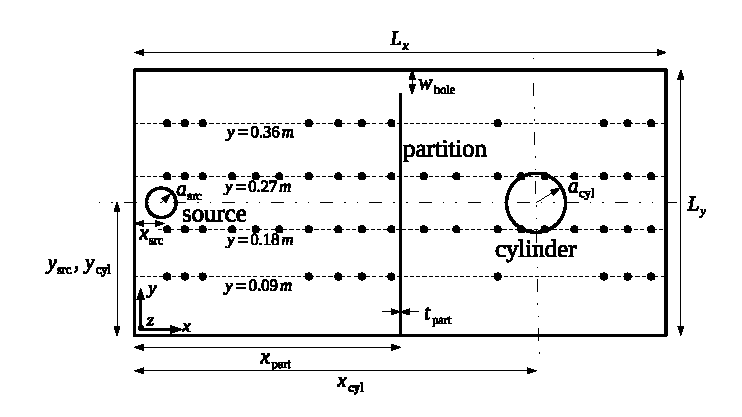
\includegraphics[width=0.8\linewidth]{figures/geometry}
\vspace{-4mm}
\caption{\label{fg:tcgeom} Cross-section in the $xy$-plane of the test case geometry.
The small black dots represent the probe locations in the z=h plane used for the measurements.}
\end{center}
\end{figure}

The cavity can also be partitioned into two sub-cavities leaving a hole of width
$w_\mathrm{hole}$ with the full height of the cavity located in the region 
$L_y-w_\mathrm{hole} \leq y \leq L_y$, $0 \leq z \leq L_z$ of the shared 
$x=x_\mathrm{part}$ wall. The hole was chosen to span the whole cavity so that the 
dimensional reduction technique is applicable and it was located along the edge of the 
partition for experimental convenience in the validation measurements.
The thickness of the partition is denoted $t_\mathrm{part}$.

The values of the parameters are given in Table~\ref{tb:tcparam}. The wall and cylinder
absorption efficiencies were chosen to match those of the physical cavity and
cylinder used for the validation measurements described in~\citep{Flintoft2017b}.
Note that the cylinder centre's $x$-coordinate is slightly different in the unpartitioned
and partitioned cavities in order to be consistent with measurement data. 

\begin{table}[ht]
\begin{center}
\begin{tabular}{|c|c|c|}
\hline
\textbf{Parameter}     &\textbf{Variable}      & \textbf{Value} \\
\hline
\multicolumn{3}{|c|}{\textbf{Geometrical}} \\
\hline
$L_x$                  &\texttt{Lx}            &0.90\,m \\
$L_y$                  &\texttt{Ly}            &0.45\,m \\
$L_z$                  &\texttt{Lz}            &0.45\,m \\
$x_\mathrm{part}$      &\texttt{partX}         &0.45\,m \\
$t_\mathrm{part}$      &\texttt{partThickness} &0.005\,m \\
$w_\mathrm{hole}$      &\texttt{holeWidth}     &0.04\,m \\
$x_\mathrm{src}$       &\texttt{srcX}          &0.05\,m \\
$y_\mathrm{src}$       &\texttt{srcY}          &0.225\,m \\
$z_\mathrm{src}$       &\texttt{srcZ}          &0.225\,m \\
$a_\mathrm{src}$       &\texttt{srcRadius}     &0.02\,m \\
$x_\mathrm{cyl}$       &\texttt{cylX}          &0.675/0.700\,m$^\mathrm{a}$ \\
$y_\mathrm{cyl}$       &\texttt{cylY}          &0.225\,m \\
$z_\mathrm{cyl}$       &\texttt{cylZ}          &0.225\,m \\
$a_\mathrm{cyl}$       &\texttt{cylRadius}     &0.05\,m \\
\hline
\multicolumn{3}{|c|}{\textbf{Electromagnetic}} \\
\hline
$P^\rt_\mathrm{src}$   &\texttt{srcTRP}        &1\,W \\
$\alpha_\mathrm{wall}$ &\texttt{wallAE}        &0.0027 \\
$\alpha_\mathrm{part}$ &\texttt{partAE}        &0.0027 \\
$\alpha_\mathrm{cyl}$  &\texttt{cylAE}         &0.95 \\
\hline
\end{tabular}
\end{center}
\caption{\label{tb:tcparam} Primary parameters and variable names for the test cases. 
$^\mathrm{a}$\texttt{cylX} is 0.7\, in the unpartitioned cavity and 0.675\,m in the
partitioned cavity.}
\end{table}

\subsection[Single and dual domain models]{Single and dual domain models}
\label{sc:tcs:sddm}

The EDM of an unpartitioned cavity can be simply implemented using a single domain model (SDM)
as shown in Figure~\ref{fg:sdm}(a). The diffusivity $D$ of the domain $\Omega$ is uniform and
the surfaces forming the walls, $\partial\Omega^\mathrm{wall}$, cylinder, $\partial\Omega^\mathrm{cyl}$, and 
possibly the source, $\partial\Omega^\mathrm{src}$, are identified. The surface bounding the source is 
used if the source is implemented as a surface or volume source, but is not used for a point source.

For coupled cavities there are a number of ways to implement the EDM. The sub-cavities can
be modelled as a single contiguous domain with the aperture between them explicitly represented in 
the geometry; this is again an SDM and is illustrated in Figure~\ref{fg:sdm}(b). The surfaces
of the walls in each sub-cavity, $\partial\Omega^\mathrm{wall}_1$ and $\partial\Omega^\mathrm{wall}_2$ are identified
and it is convenient to also explicitly identify the portions of the partition surface which face into
each sub-cavity, $\partial\Omega^\mathrm{part}_1$ and $\partial\Omega^\mathrm{part}_2$. While only a single domain
is modelled an inhomogeneous diffusivity is used to assign the appropriate diffusivities $D_1$ and
$D_2$ in each sub-cavity:
\begin{align}
D(\vr) = \left\{ 
\begin{matrix}
D_1    &x <= x_\mathrm{part} \\
D_2    &x > x_\mathrm{part} 
\end{matrix}
\right.\,.
\end{align}
The energy density through the hole in this case satisfies the natural continuity boundary conditions
for its value and derivative.

\begin{figure}[ht]
\begin{center}
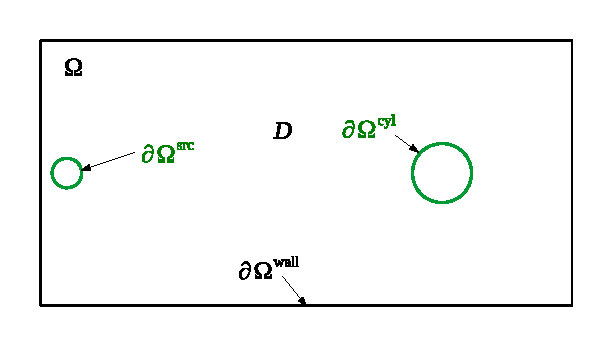
\includegraphics[width=0.6\linewidth]{figures/domains0}\\
{\footnotesize (a)}\\
\vspace{-4mm}
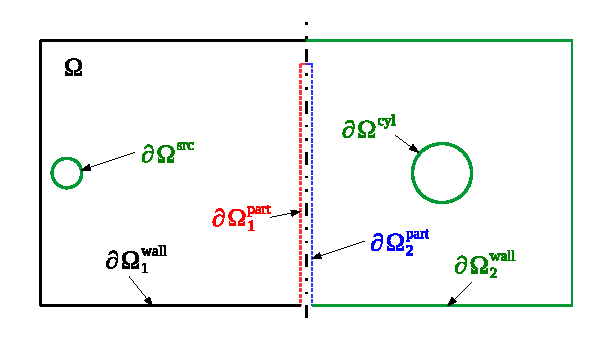
\includegraphics[width=0.6\linewidth]{figures/domains1}\\
{\footnotesize (b)}\\
\vspace{0mm}
\caption{\label{fg:sdm} Domain nomenclature for the single domain model (SDM) implementation of the 
single cavity (a) and partitioned cavity (b).}
\end{center}
\end{figure}

Alternatively the partitioned cavity can be implemented as a dual domain model (DDM) as shown in
Figure~\ref{fg:ddm}, in which the sub-cavities are represented as completely separate domains 
$\Omega_1$ and $\Omega_2$. The surface corresponding to the hole is meshed as part of the surface
bounding each sub-cavity and identified as $\partial\Omega^\mathrm{hole}_{12}$ and $\partial\Omega^\mathrm{hole}_{21}$ in 
the source and coupled sub-cavities respectively. The diffusivity in each sub-cavity is homogeneous
with values $D_1$ and $D_2$ respectively. A appropriate boundary condition must be applied on the 
surfaces $\partial\Omega^\mathrm{hole}_{12}$ and $\partial\Omega^\mathrm{hole}_{21}$:
\begin{itemize}
 \item \textbf{EEBC}: Exchange coefficients are used to enforce Robin BCs according to~(\ref{eq:eebc1})-(\ref{eq:eebc2}).
 \item \textbf{FCBC}: The energy density flux is forced to be continuous through the hole using~(\ref{eq:fcbc}). For lossless apertures
 with unity transmission efficiency this is equivalent to the EEBC; 
 \item \textbf{Schwarz}: A non-overlapping Schwarz algorithm can be applied which enforces continuity of both
 the energy density and its flux; this is equivalent to using an SDM;
\end{itemize}
The SDM/Schwarz approach implicitly assumes that the aperture is electrical large and may only be accurate in this
regime. The EEBC/FCBC method allow discontinuity of the energy density across aperture, which may be more appropriate 
for apertures which are in the resonant regime. For electrically small apertures the EEBC approach must be used and the 
appropriate transmission efficiency (TE) included. These conjectures on the realm of validity of the different aperture modelling approaches
require verification, either by experiment or using full-wave simulation.

\begin{figure}[ht]
\begin{center}
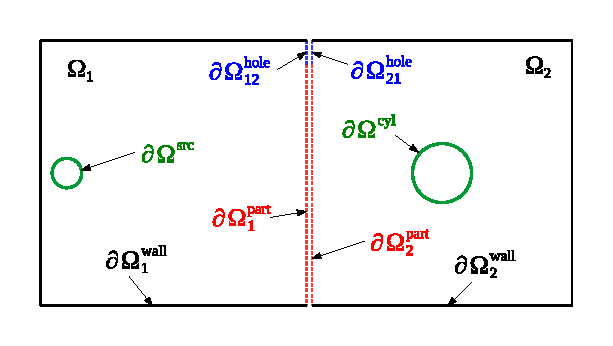
\includegraphics[width=0.6\linewidth]{figures/domains2}
\vspace{-4mm}
\caption{\label{fg:ddm} Domain nomenclature for the dual domain model (DDM) implementation of the partitioned cavity.}
\end{center}
\end{figure}

\subsection[Overall solution work-flow]{Overall solution work-flow}
\label{sc:tcs:workflow}

The overall solution of the EDM is implemented using a combination of Open Source tools: 
\begin{enumerate}
 \item \textbf{Gmsh}: For 3D solutions a parametric CAD model of the geometry is created using 
 Gmsh~\citep{Geuzaine2009}. Gmsh is then used to created a tetrahedral mesh from this CAD model, which 
 is then exported using the INRIA Medit format. As an example, the mesh for the loaded partitioned cavity
 is shown in Figure~\ref{fg:tcdualmesh}.
 \item \textbf{FreeFEM++}: The FEM solution is determined using FreeFEM++~\citep{Hecht2013}. For 2D
 solutions the mesh is created directly within FreeFEM++, while for 3D solutions the mesh is imported in INRIA
 Medit format. The resulting energy density and energy density flux are exported in sampled form to ASCII files. 
 \item \textbf{Octave}: Post-processing is carried out by importing the sampled energy density and energy density 
 flux into GNU Octave. The post-processing scripts are compatible with MATLAB.
\end{enumerate}

\begin{figure}[ht]
\begin{center}
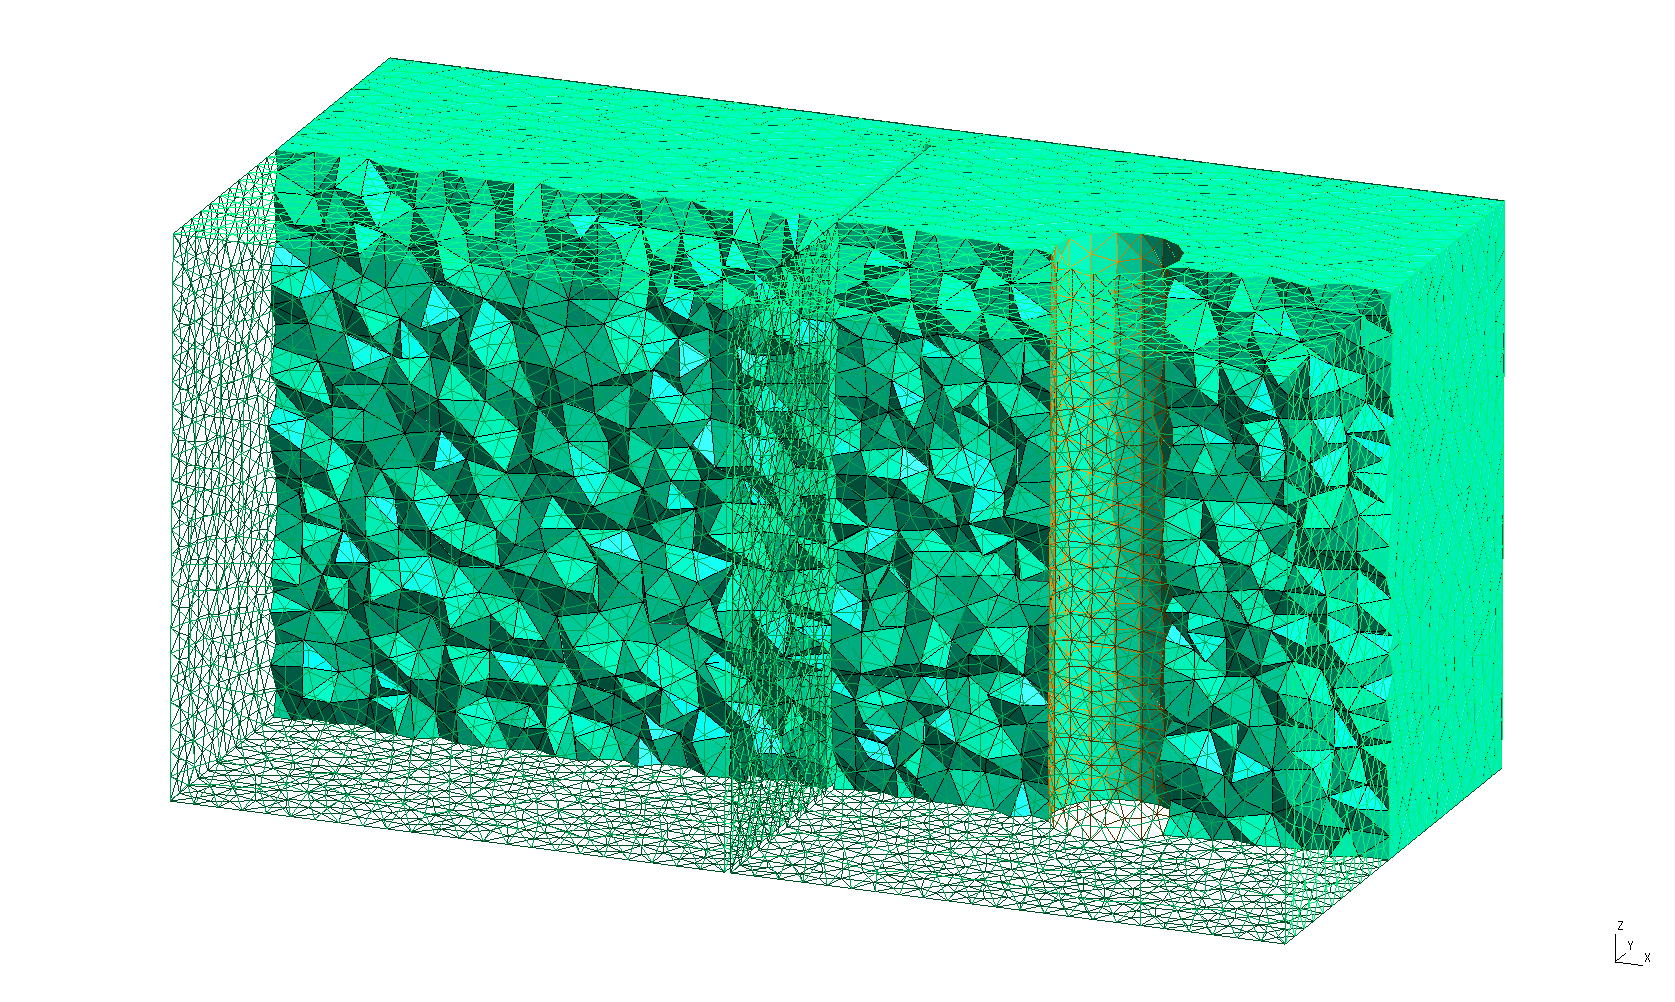
\includegraphics[width=0.8\linewidth]{figures/gmshdualmesh}
\vspace{-4mm}
\caption{\label{fg:tcdualmesh} Tetrahedral mesh of the coupled cavities test-case containing the lossy cylinder.}
\end{center}
\end{figure}

The input for Gmsh, FreeFEM++ and Octave is all taken from the same ASCII text file \texttt{parameters.geo}, which
is in Gmsh's ``geo'' format. The file contains a series of lines, each of which assigns a value to a variable:
{\small
\begin{verbatim}
isSrc = 0;             // Whether to mesh the source as a spherical surface [0/1].
isCyl = 1;             // Whether to include the cylinder [0/1].
isPart = 1;            // Whether to include the partition [0/1].
isSabine = 1;          // Whether to use Sabine or Jing & Xiang absorption factor model [0/1].
Lx = 0.9;              // Cavity size in x-direction [m].
Ly = 0.45;             // Cavity size in y-direction [m].
Lz = 0.45;             // Cavity size in z-direction [m].
wallAE = 0.0027;       // Absorption efficiency of walls [-].
partX = 0.45;          // x-coordinate of partition [m].
partThickness = 0.005; // Partition thickness [m].
partAE = 0.0027;       // Absorption efficiency of partition [-].
holeWidth = 0.04;      // Aperture width [m].
holeTE = 1.0;          // transmission efficiency of hole [-].
cylXWithPart = 0.675;  // x-coordinate of cylinder if partition is present [m].
cylXWithoutPart = 0.7; // x-coordinate of cylinder if partition is not present [m].
cylY = 0.225;          // y-coordinate of cylinder [m].
cylRadius = 0.05;      // Cylinder radius [m].
cylAE = 0.95;          // Absorption efficiency of cylinder [-].
srcX = 0.05;           // x-coordinates of source [m].
srcY = 0.225;          // y-coordinates of source [m].
srcZ = 0.225;          // z-coordinates of source [m].
srcRadius = 0.02;      // Source radius if meshed as sphere [m].
srcTRP = 1;            // Total radiated power of source [W].
\end{verbatim}}
\noindent In order for FreeFEM++ and Octave to be able to parse the file correctly it is essential 
that spaces are left on either side of the ``\texttt{=}'' sign. The order of the parameters is 
not significant. 

In addition to the geometrical and electromagnetic parameters defined in 
Table~\ref{tb:tcparam} four boolean parameters \texttt{isSrc}, \texttt{isCyl}, \texttt{isPart} and 
\texttt{isSabine} are also used:
\begin{itemize}
 \item \textbf{\texttt{isSrc}}: If true, a small sphere is added to the mesh to represent the source using a surface,
 otherwise an interpolated delta function source is applied;
 \item \textbf{\texttt{isCyl}}: If true, the cylinder is included in the geometry;
 \item \textbf{\texttt{isPart}}: If true, the partition is included;
 \item \textbf{\texttt{isSabine}}: If true, the Sabine EC~(\ref{eq:ecsabine}) is used,
 otherwise the Jing and Xiang EC~(\ref{eq:ecjing}) is used.
\end{itemize}

\section[Results]{Results}
\label{sc:res}

EDM results are presented in Sections~\ref{sc:res:unpartempty} to~\ref{sc:res:cylpart} for baseline canonical 
test cases with the following parameters:
\begin{itemize}
 \item The Sabine EC~(\ref{eq:ecsabine}) is used for all surfaces;
 \item For the loaded cases the diffusivity is determined using~(\ref{eq:harmmean});
 \item The specularity factor~(\ref{eq:kappa}) is taken to be unity.
\end{itemize}
For coupled cavities results are reported for SDM and EEBC DDM methods. In each case it was verified
that the FCBC and EEBC DDM gave the same results and likewise for the SDM and non-overlapping Schwarz
DDM. Generally the FCBC and EEBC agreed to within the convergence tolerance requested (0.1\,\%) in the 
total energy density while the agreement between the SDM and Schwarz DDM was very slightly worse than
the requested tolerance, which is due to the differences in the meshes. Derived parameters common 
to all the canonical test-case models are given in Table~\ref{tb:derivparams}.

\begin{table}[ht]
\begin{center}
\begin{tabular}{|c|c|c|}
\hline
\textbf{Parameter}     &\textbf{Unit} &\textbf{Value}\\ 
\hline
\texttt{wallEC}        &m/s           &2.0236$\times 10^5$ \\
\texttt{cylEC}         &m/s           &7.1201$\times 10^7$ \\
\texttt{partEC}        &m/s           &2.0236$\times 10^5$ \\
\texttt{holeEC}        &m/s           &7.4948$\times 10^7$ \\
\texttt{holeArea}      &m$^2$         &0.018000            \\
\texttt{holeTCS}       &m$^2$         &0.0045000           \\
\texttt{cylArea}       &m$^2$         &0.14137             \\
\texttt{cylACS}        &m$^2$         &0.033576            \\
\hline
\end{tabular}
\end{center}
\caption{\label{tb:derivparams} Common derived parameters for the test-cases.}
\end{table}

\subsection[Empty unpartitioned cavity]{Empty unpartitioned cavity}
\label{sc:res:unpartempty}

The derived parameters for the empty unpartitioned cavity are given in Table~\ref{tb:derivparamsu} and the summary 
statistics for the average power density in the EDM models are presented in Table~\ref{tb:unpartempty}. 
Results are given for 2D and 3D SDM cases and also for the homogeneous PWB model. The power density is very 
uniform, with a coefficient of variation (COV) of about 0.6\,\%. All the models are in close agreement 
as expected, since the loss in the cavity is very low.

\begin{table}[ht]
\begin{center}
\begin{tabular}{|c|c|c|}
\hline
\textbf{Parameter}     &\textbf{Unit} &\textbf{Value}\\ 
\hline
\texttt{wallArea}      &m$^2$         &2.025              \\
\texttt{cavityArea}    &m$^2$         &2.025              \\
\texttt{cavityVolume}  &m$^3$         &0.18225            \\
\texttt{wallMFP}       &m             &0.36               \\
\texttt{cavityMFP}     &m             &0.36               \\
\texttt{wallD}         &m$^2$/s       &3.5975$\times10^7$ \\
\texttt{cavityD}       &m$^2$/s       &3.5975$\times10^7$ \\
\texttt{wallACS}       &m$^2$         &0.0013669          \\
\texttt{cavityACS}     &m$^2$         &0.0013669          \\
\hline
\end{tabular}
\end{center}
\caption{\label{tb:derivparamsu} Derived parameters for the unpartitioned empty cavity.}
\end{table}

\begin{table}[ht]
\begin{center}
\begin{tabular}{|l|c|c|c|c|c|}
\hline
\textbf{Power density}               &\textbf{PWB} &\multicolumn{2}{|c|}{\textbf{EDM}} \\ \cline{3-4}
{}                                   &{}           &\textbf{2D SDM} &\textbf{3D SDM}  \\
\hline
Value at centre (dB\,W\,m$^{-2})$    &28.64        &28.63           &28.63 \\
Mean (dB\,W\,m$^{-2})$               &28.64        &28.63           &28.63 \\
Minimum (dB\,W\,m$^{-2})$            &28.64        &28.60           &28.03 \\
Maximum (dB\,W\,m$^{-2})$            &28.64        &28.71           &28.74 \\
Standard deviation (dB\,W\,m$^{-2})$ &0            &6.50            &6.17  \\
Coefficient of variation (\%)        &0            &0.61            &0.57  \\
\hline
\end{tabular}
\end{center}
\caption{\label{tb:unpartempty} Statistics of the reverberant power density in the unpartitioned empty cavity.}
\end{table}

\begin{figure}[hp]
\begin{center}
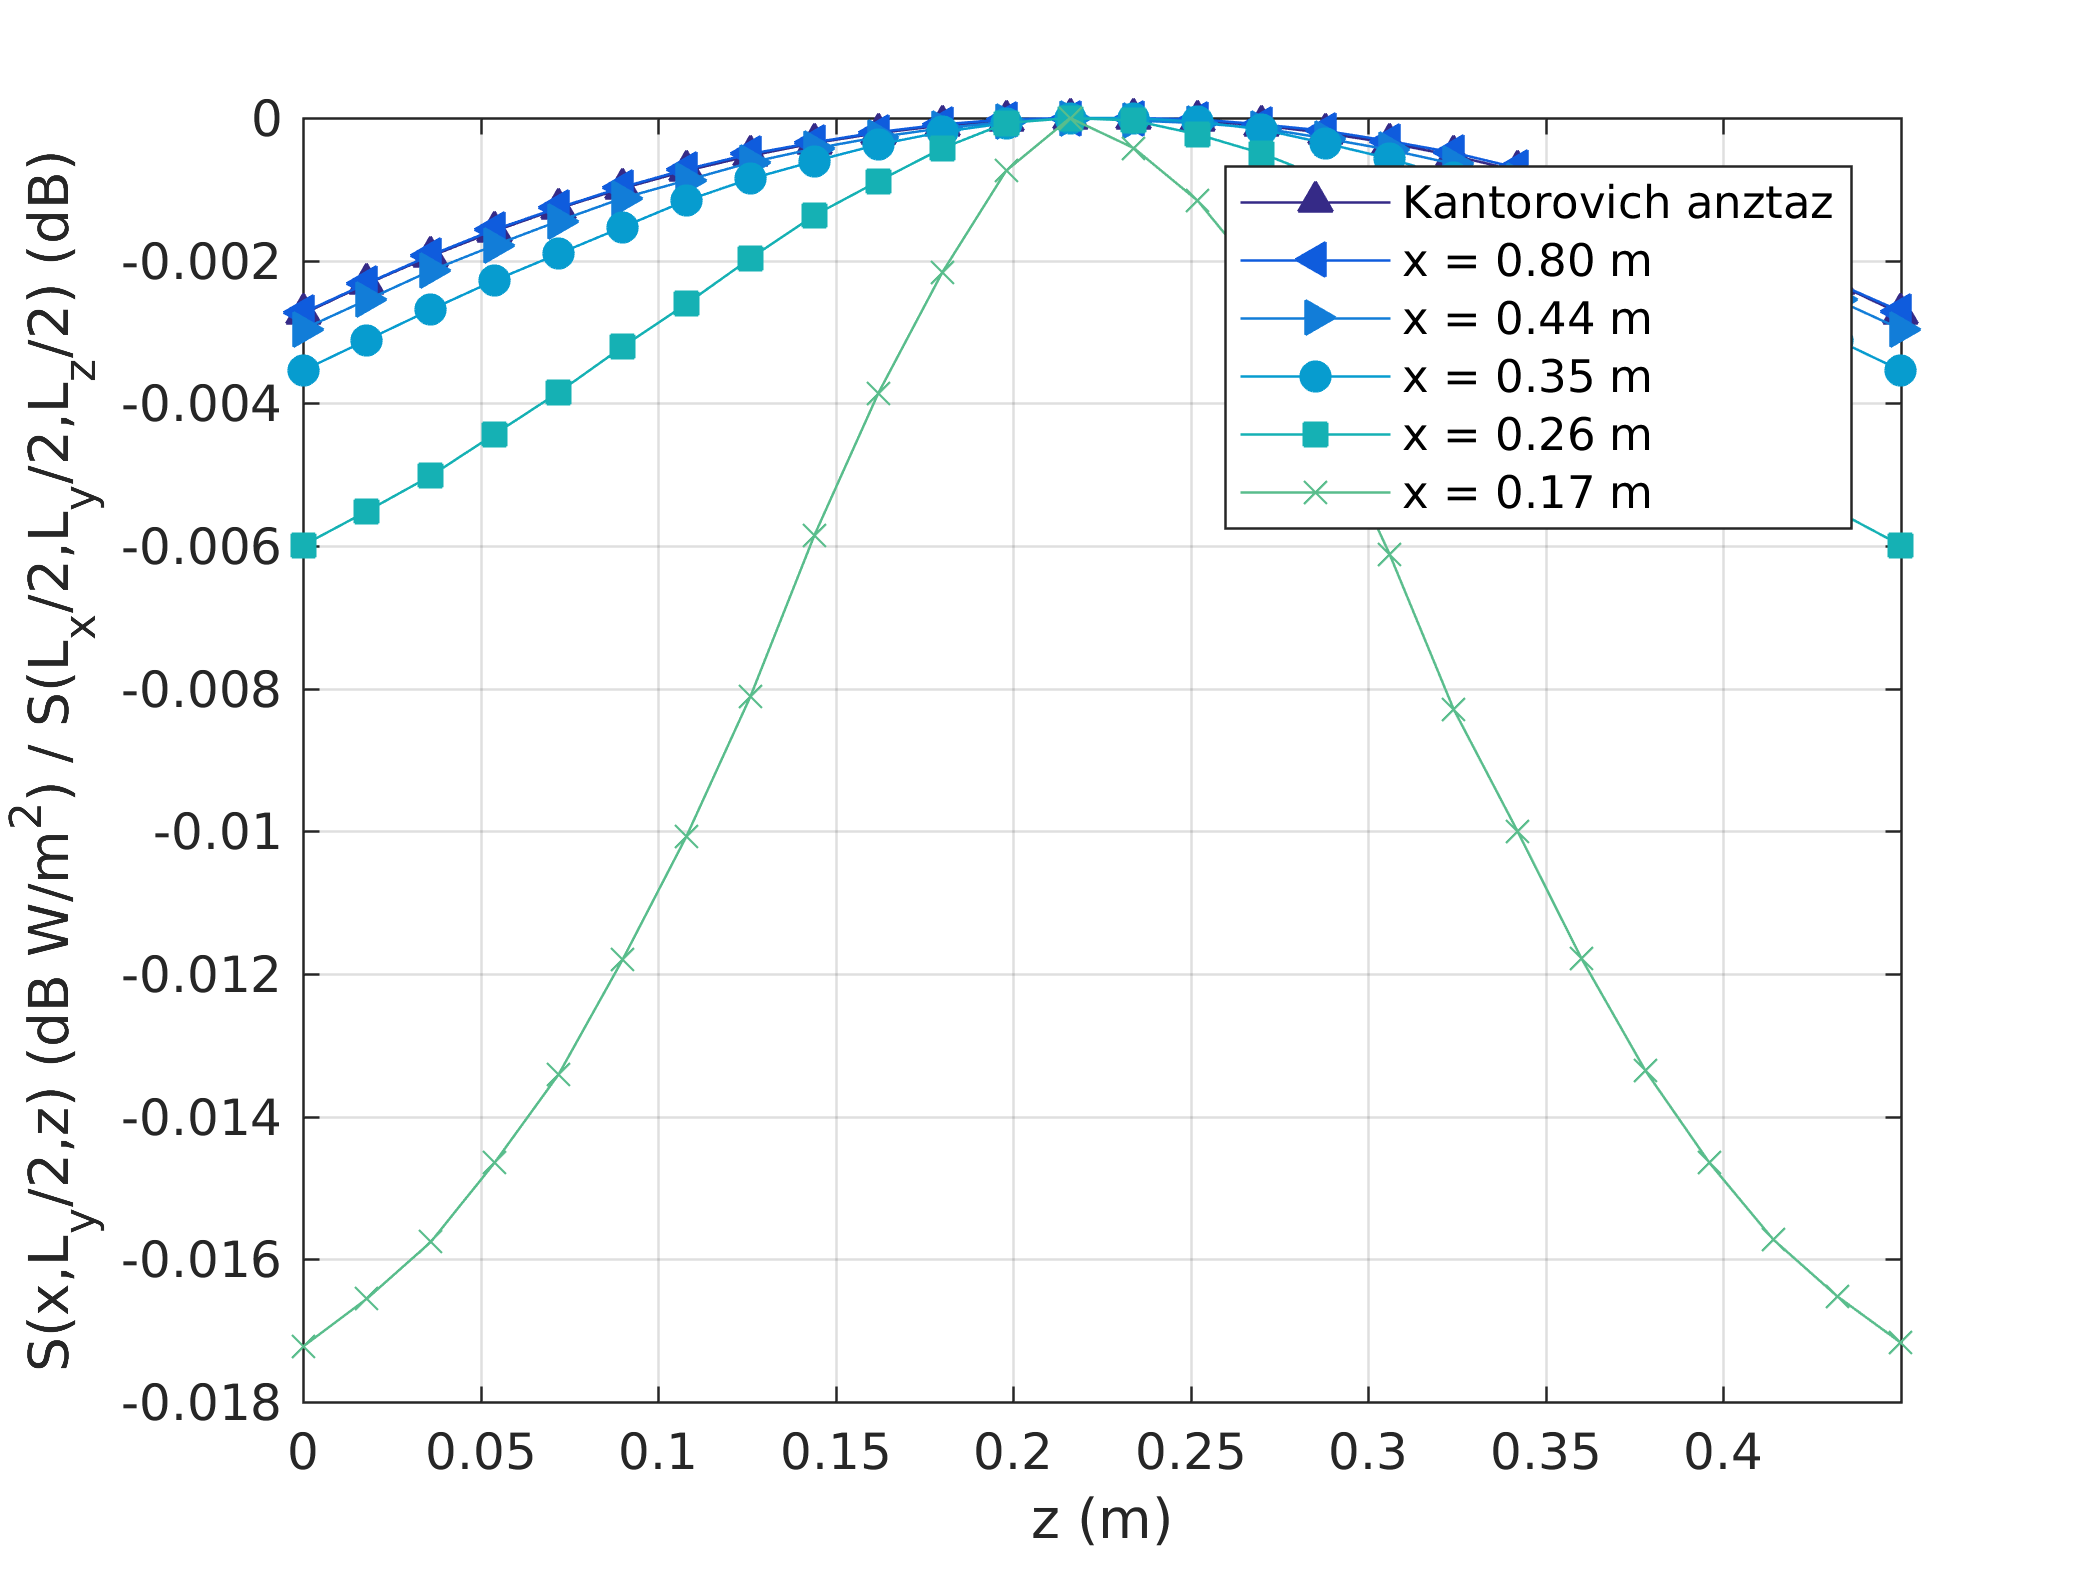
\includegraphics[width=0.6\linewidth]{figures/SDM_3D_SU_PowerDensityProfileZ}\\
{\footnotesize (a)}\\
\vspace{2mm}
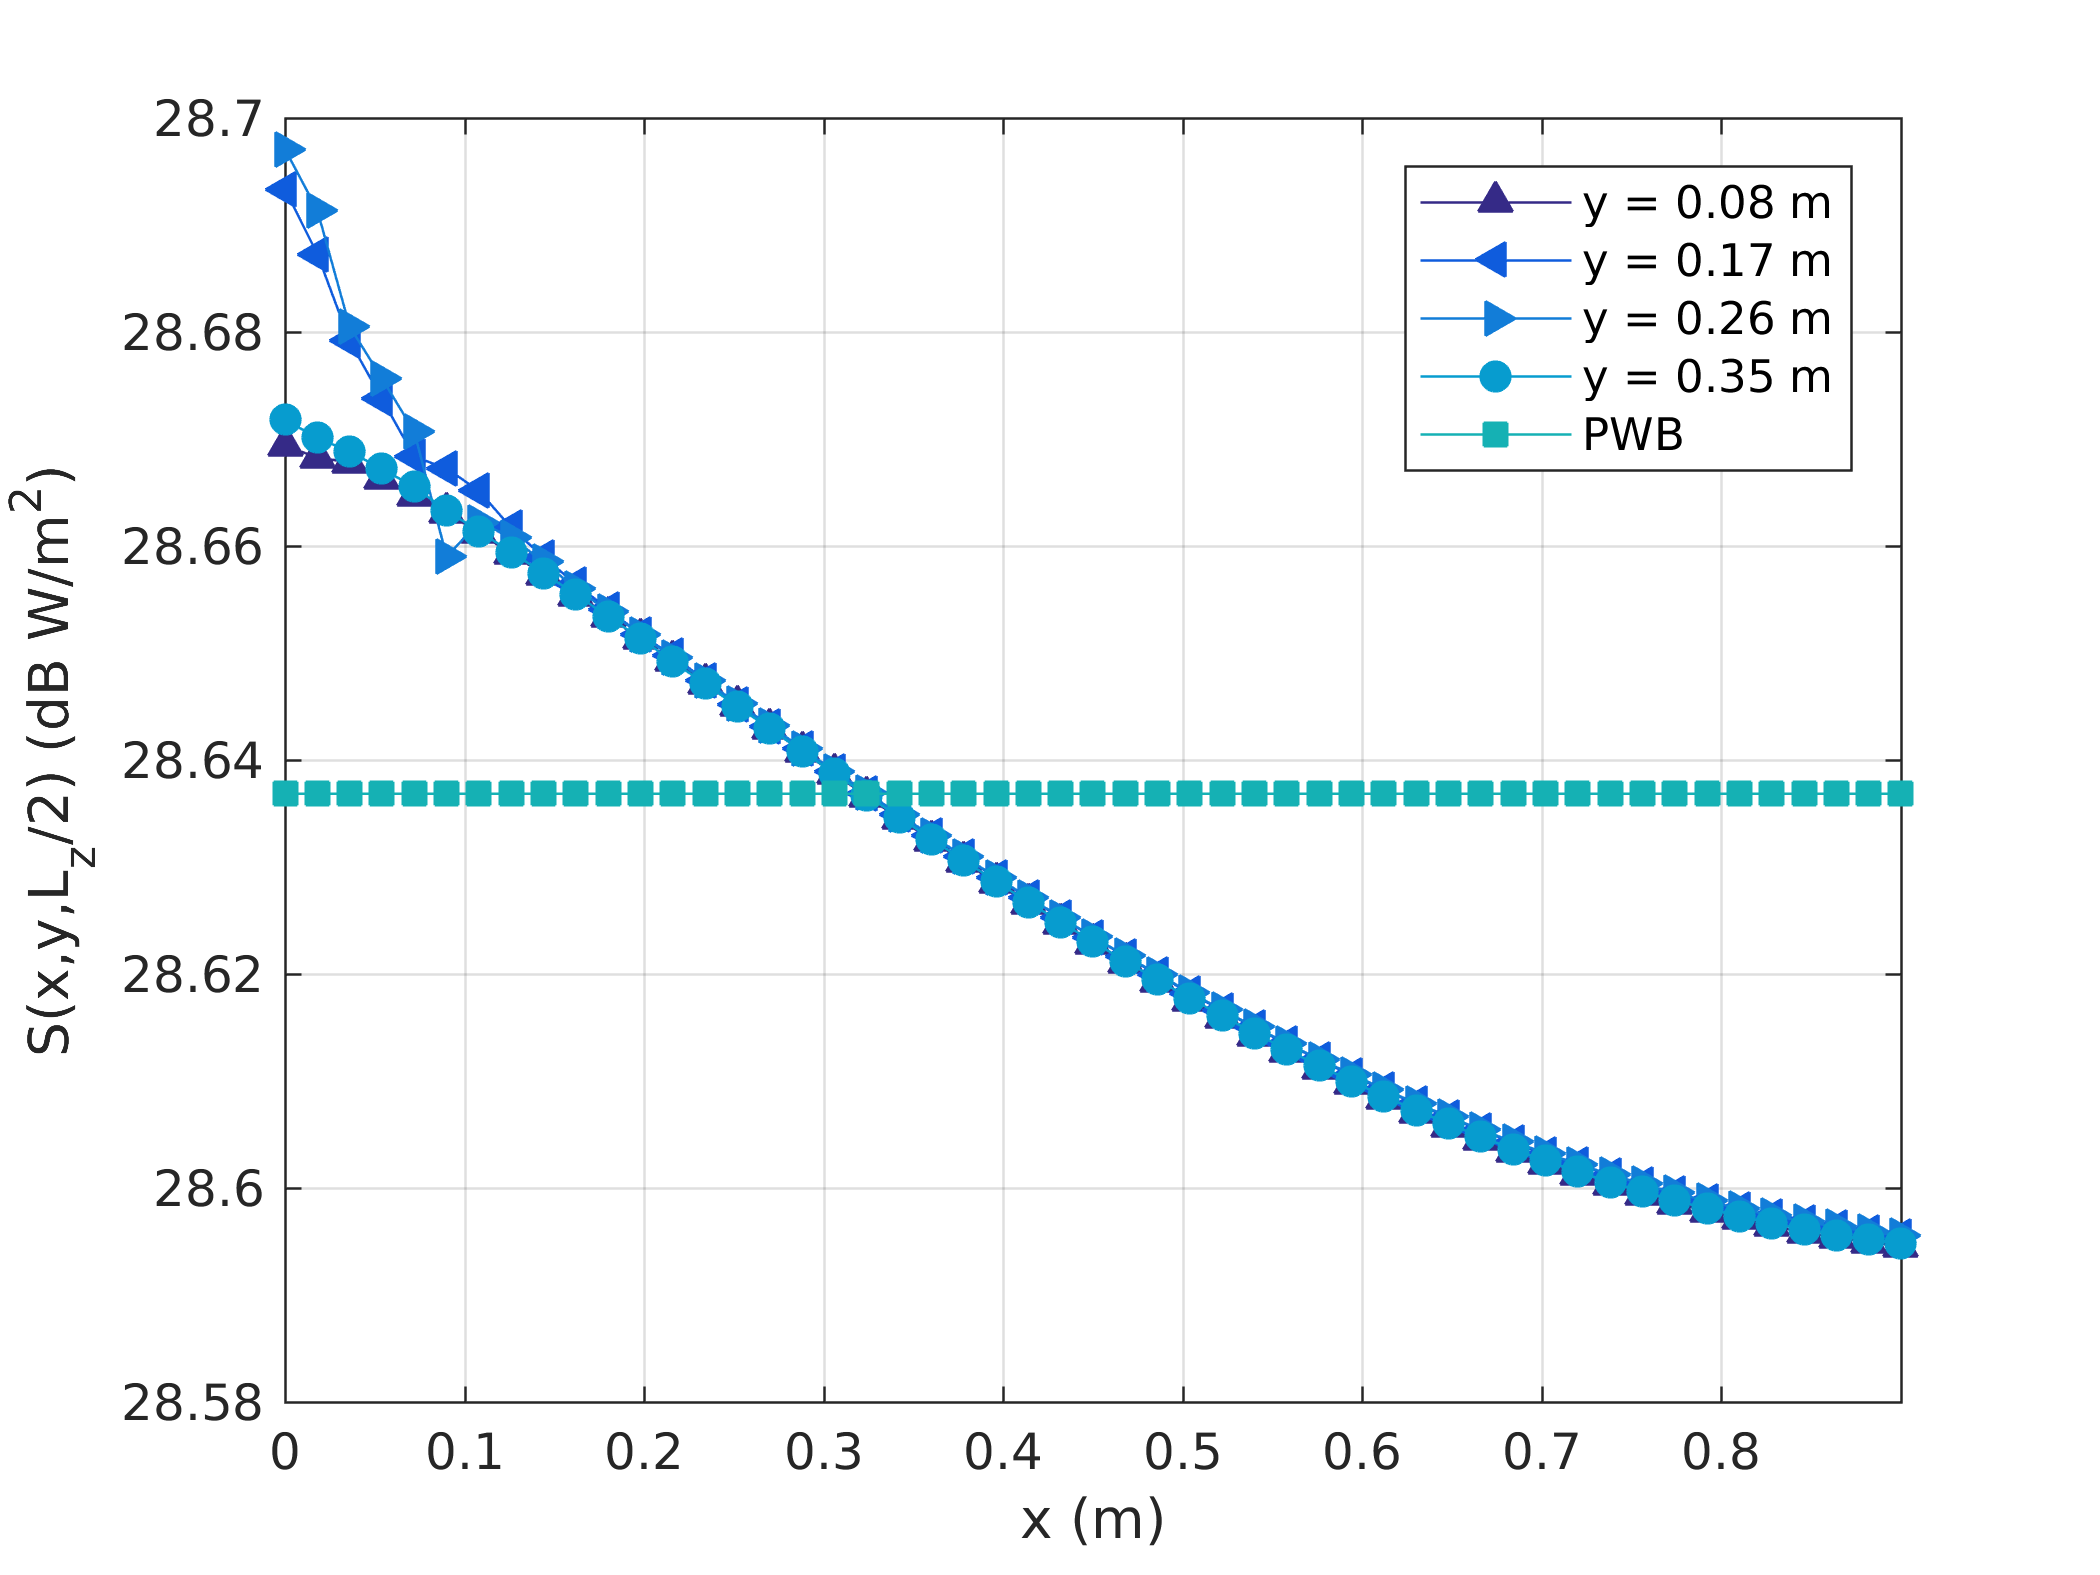
\includegraphics[width=0.6\linewidth]{figures/SDM_3D_SU_PowerDensityProfileX}\\
{\footnotesize (b)}\\
\vspace{2mm}
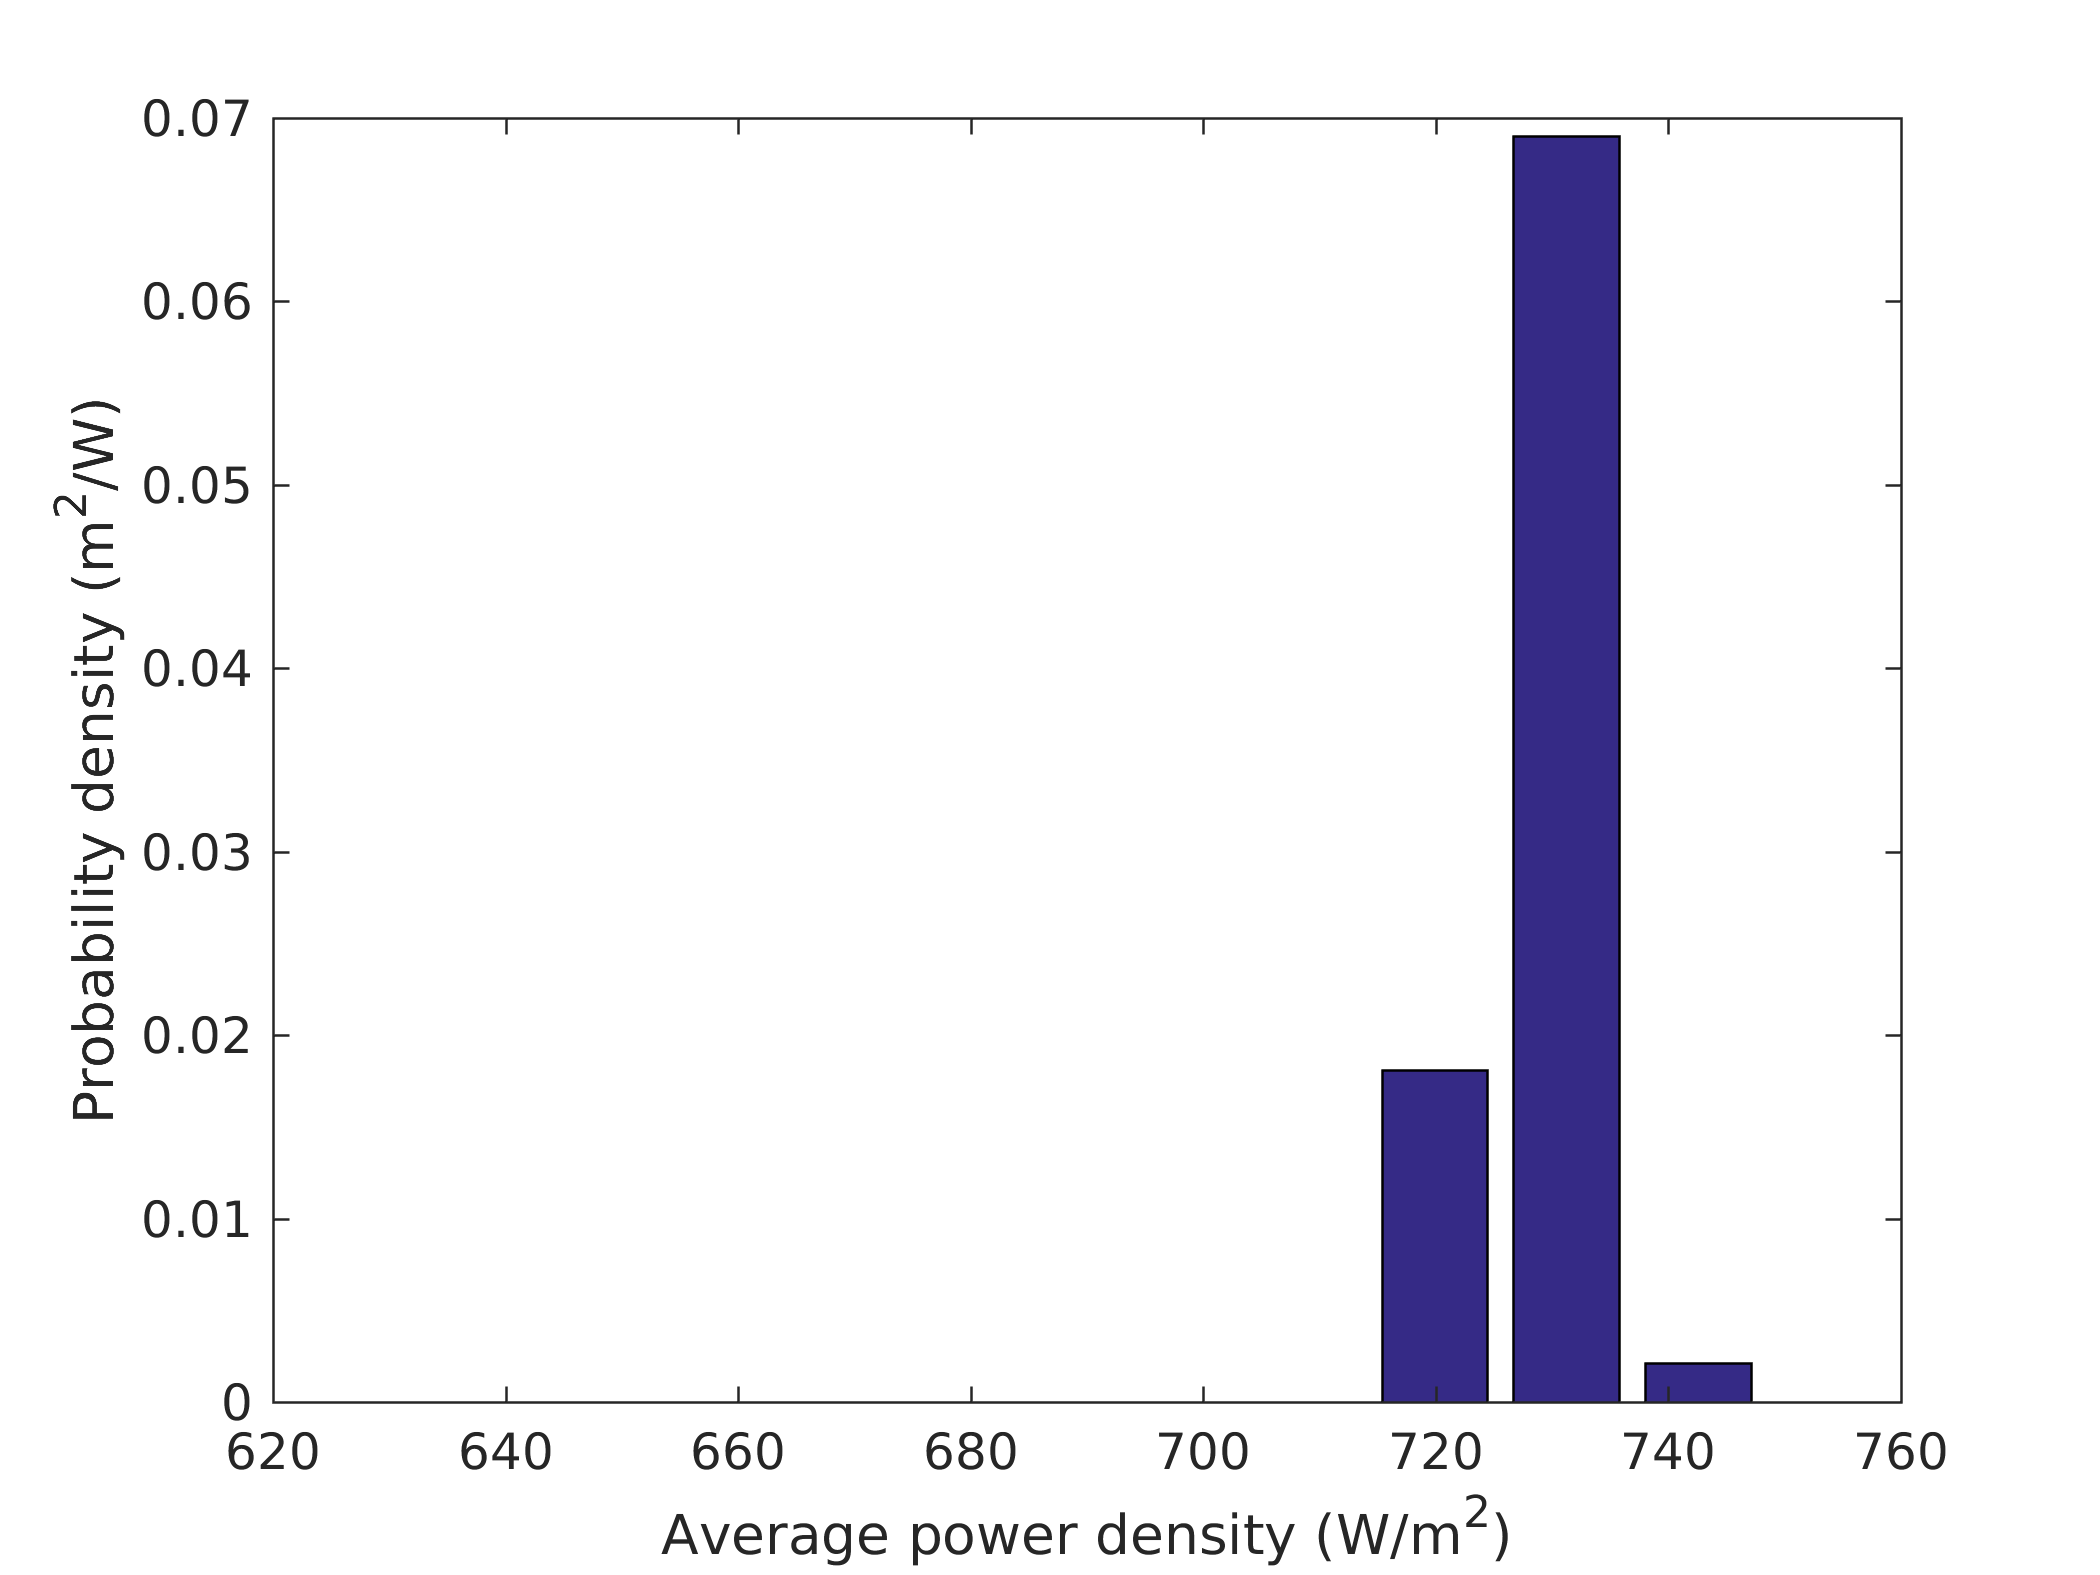
\includegraphics[width=0.6\linewidth]{figures/SDM_3D_SU_PowerDensityPDF}\\
{\footnotesize (c)}\\
\vspace{-2mm}
\caption{\label{fg:unpartempty_profs} EDM of the unloaded unpartitioned cavity: (a) Normalised vertical profile of the power density; 
(b) Power density profile in the $x$-direction along the cavity centre; (c) PDF of the power density throughout the cavity volume.}
\end{center}
\end{figure}

\begin{figure}[hp]
\begin{center}
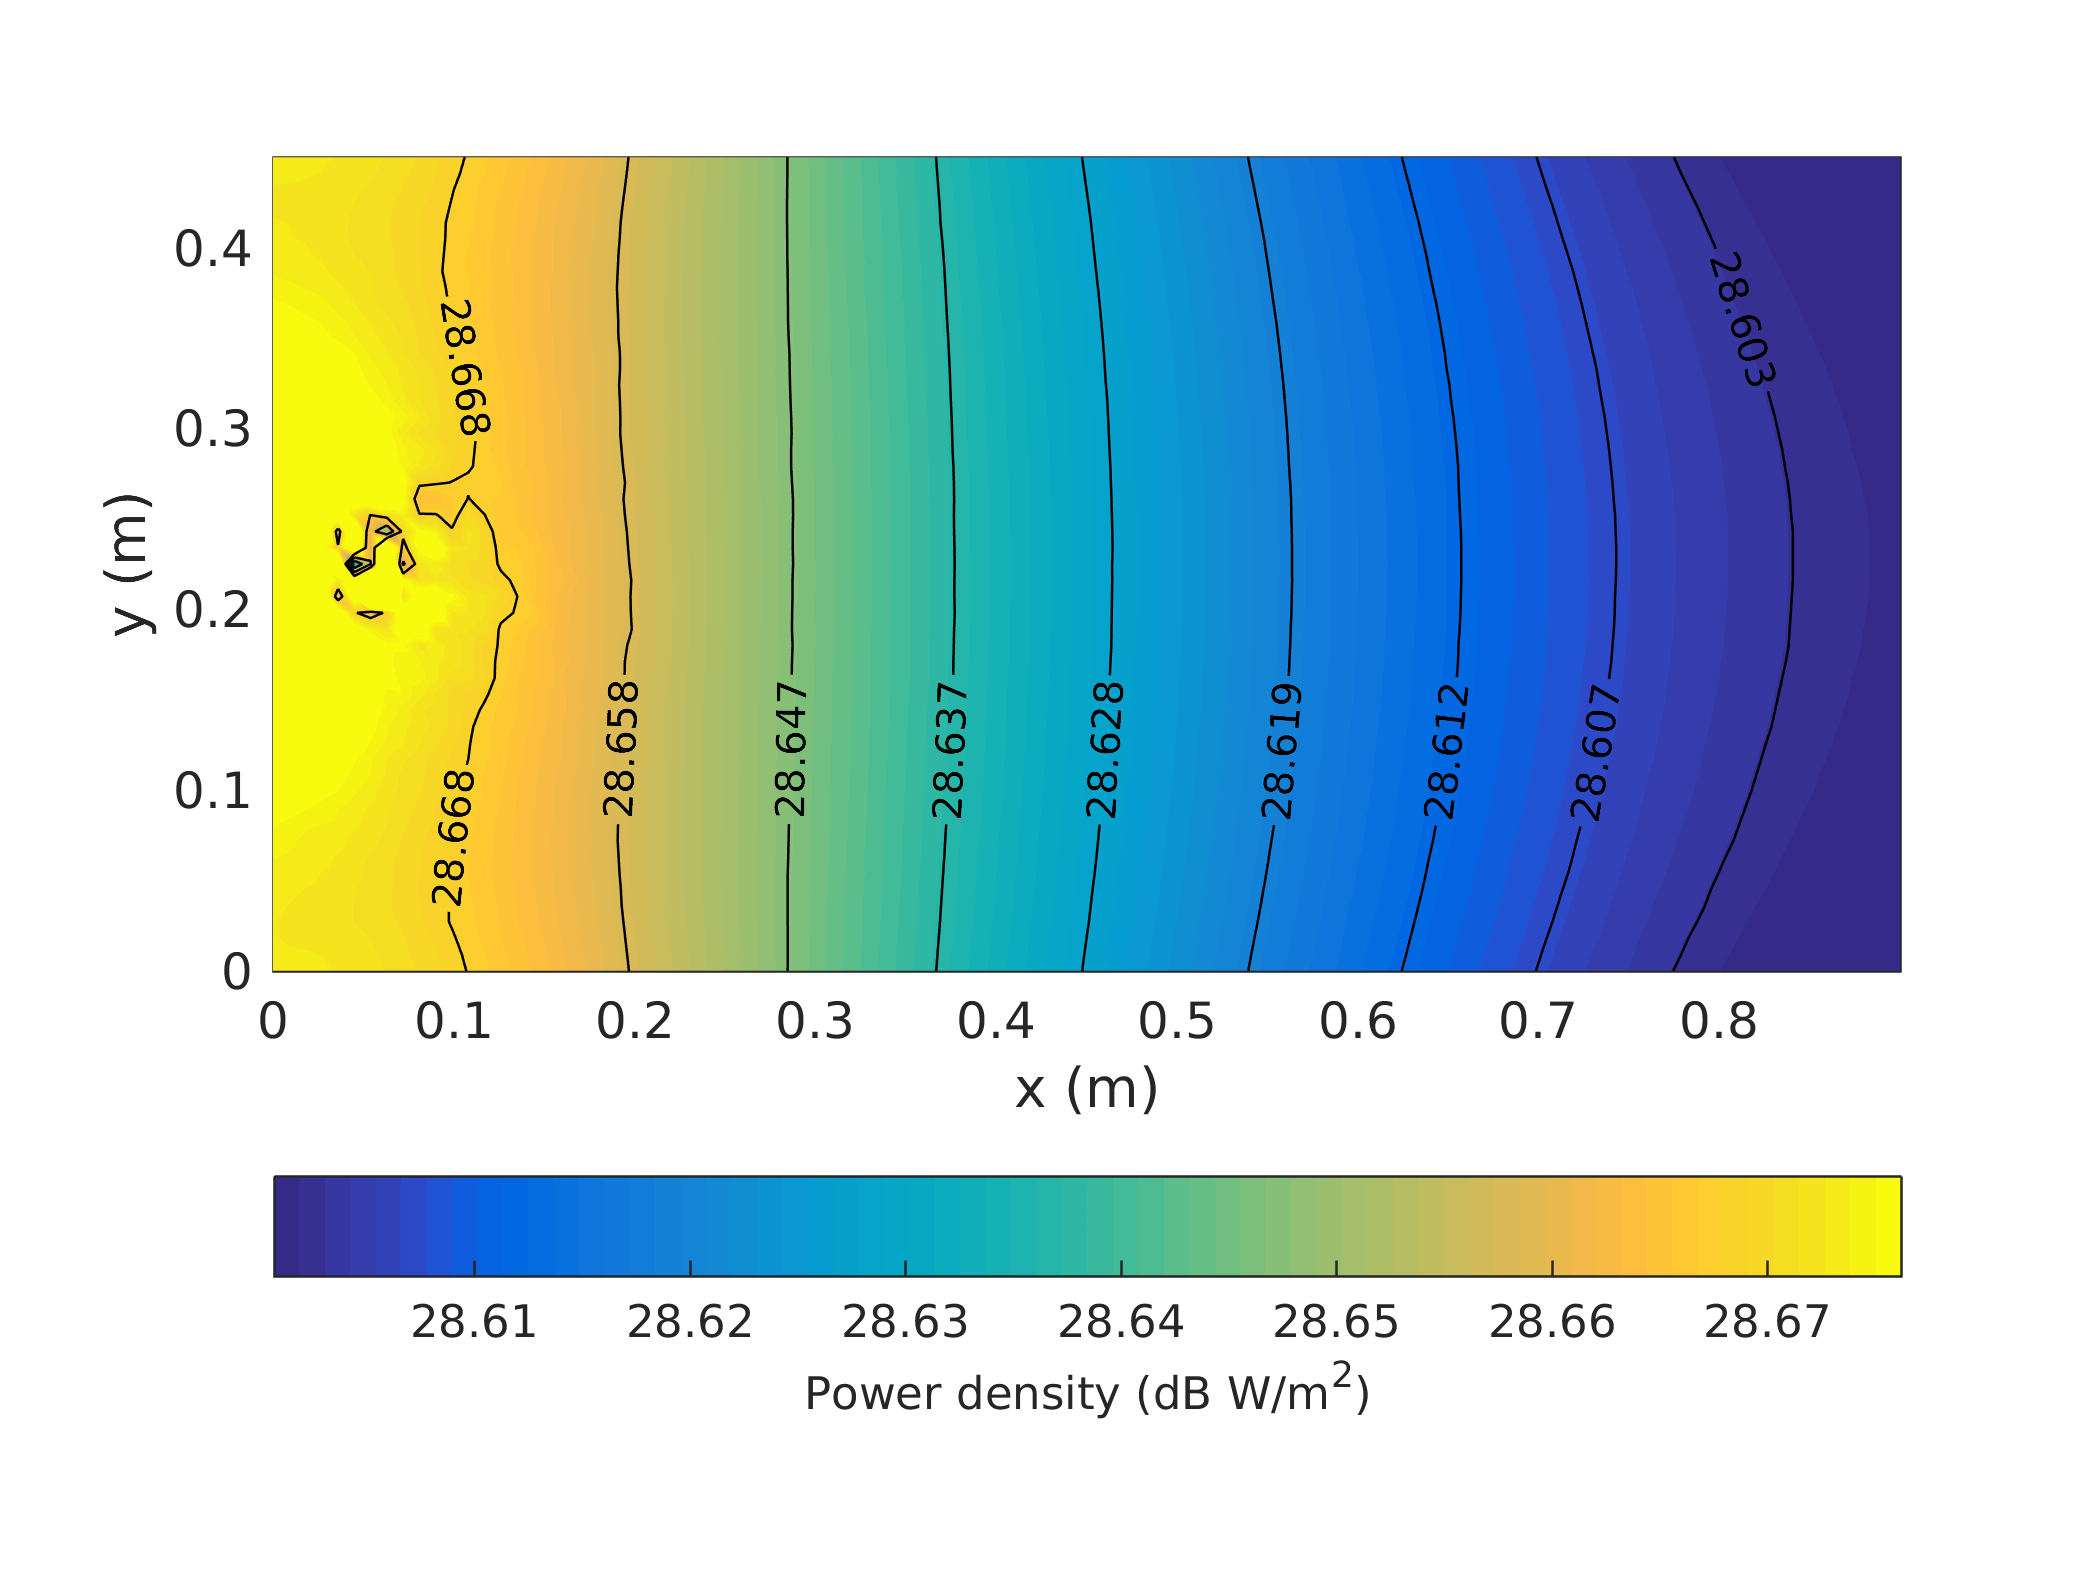
\includegraphics[trim={0 8mm 0 12mm},clip,width=0.52\linewidth]{figures/SDM_3D_SU_PowerDensityMap}\\
{\footnotesize (a)}\\
\vspace{2mm}
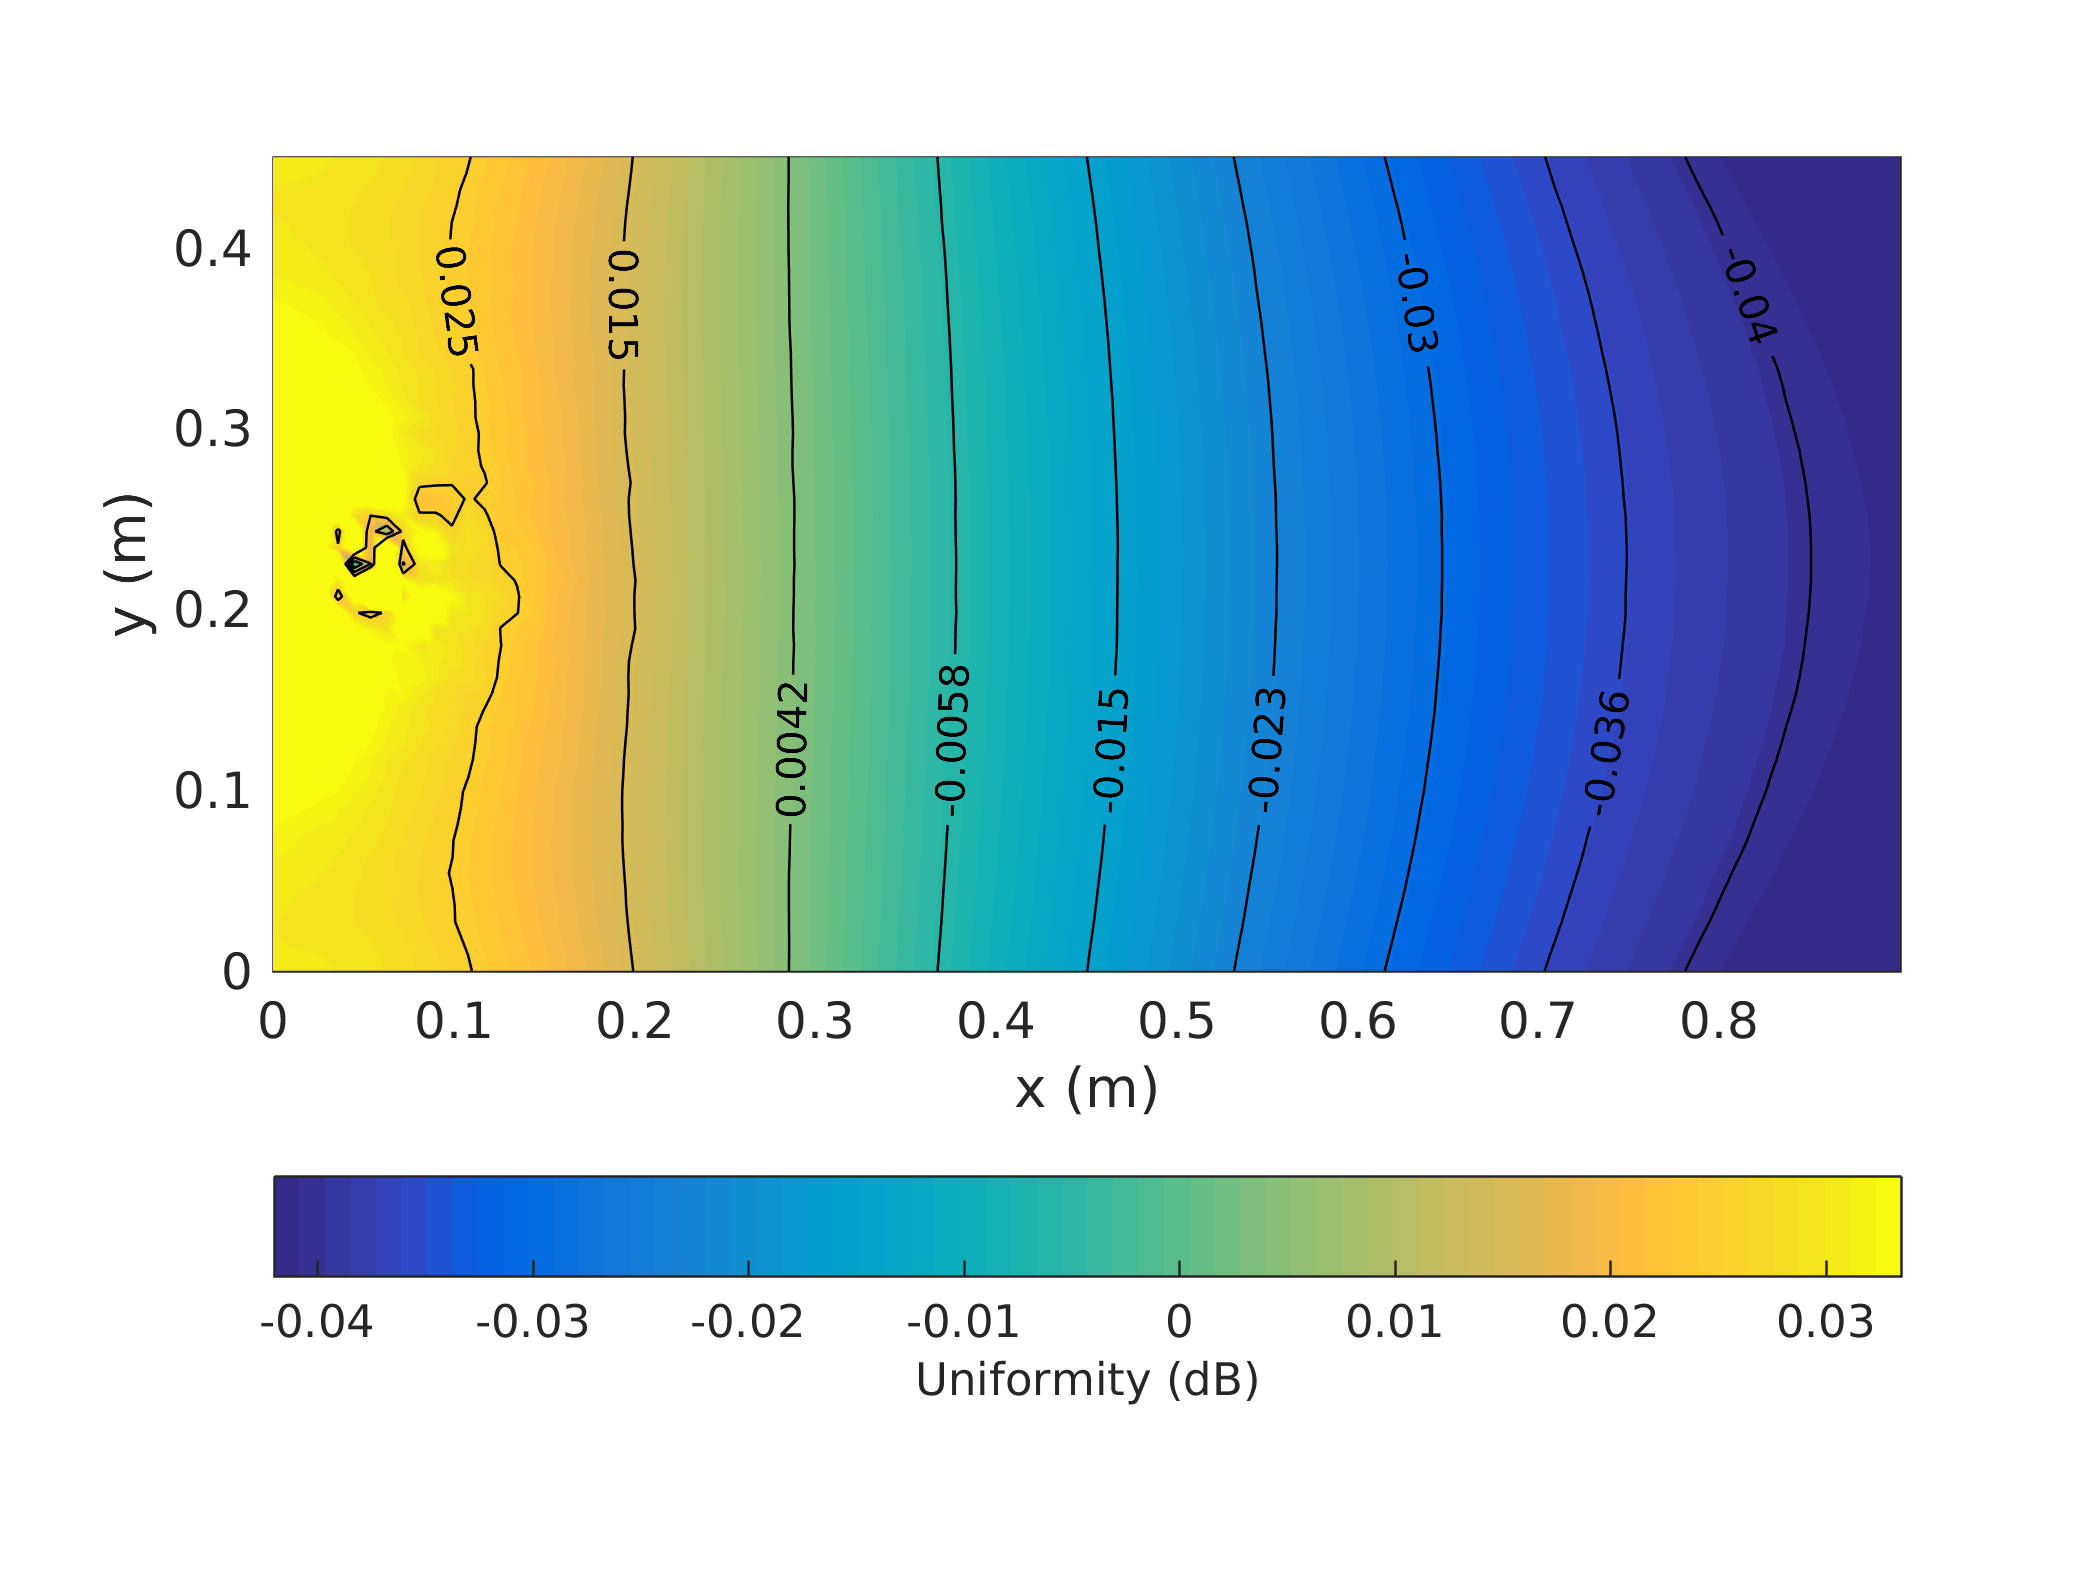
\includegraphics[trim={0 8mm 0 12mm},clip,width=0.52\linewidth]{figures/SDM_3D_SU_EnergyDensityUniformityMap}\\
{\footnotesize (b)}\\
\vspace{2mm}
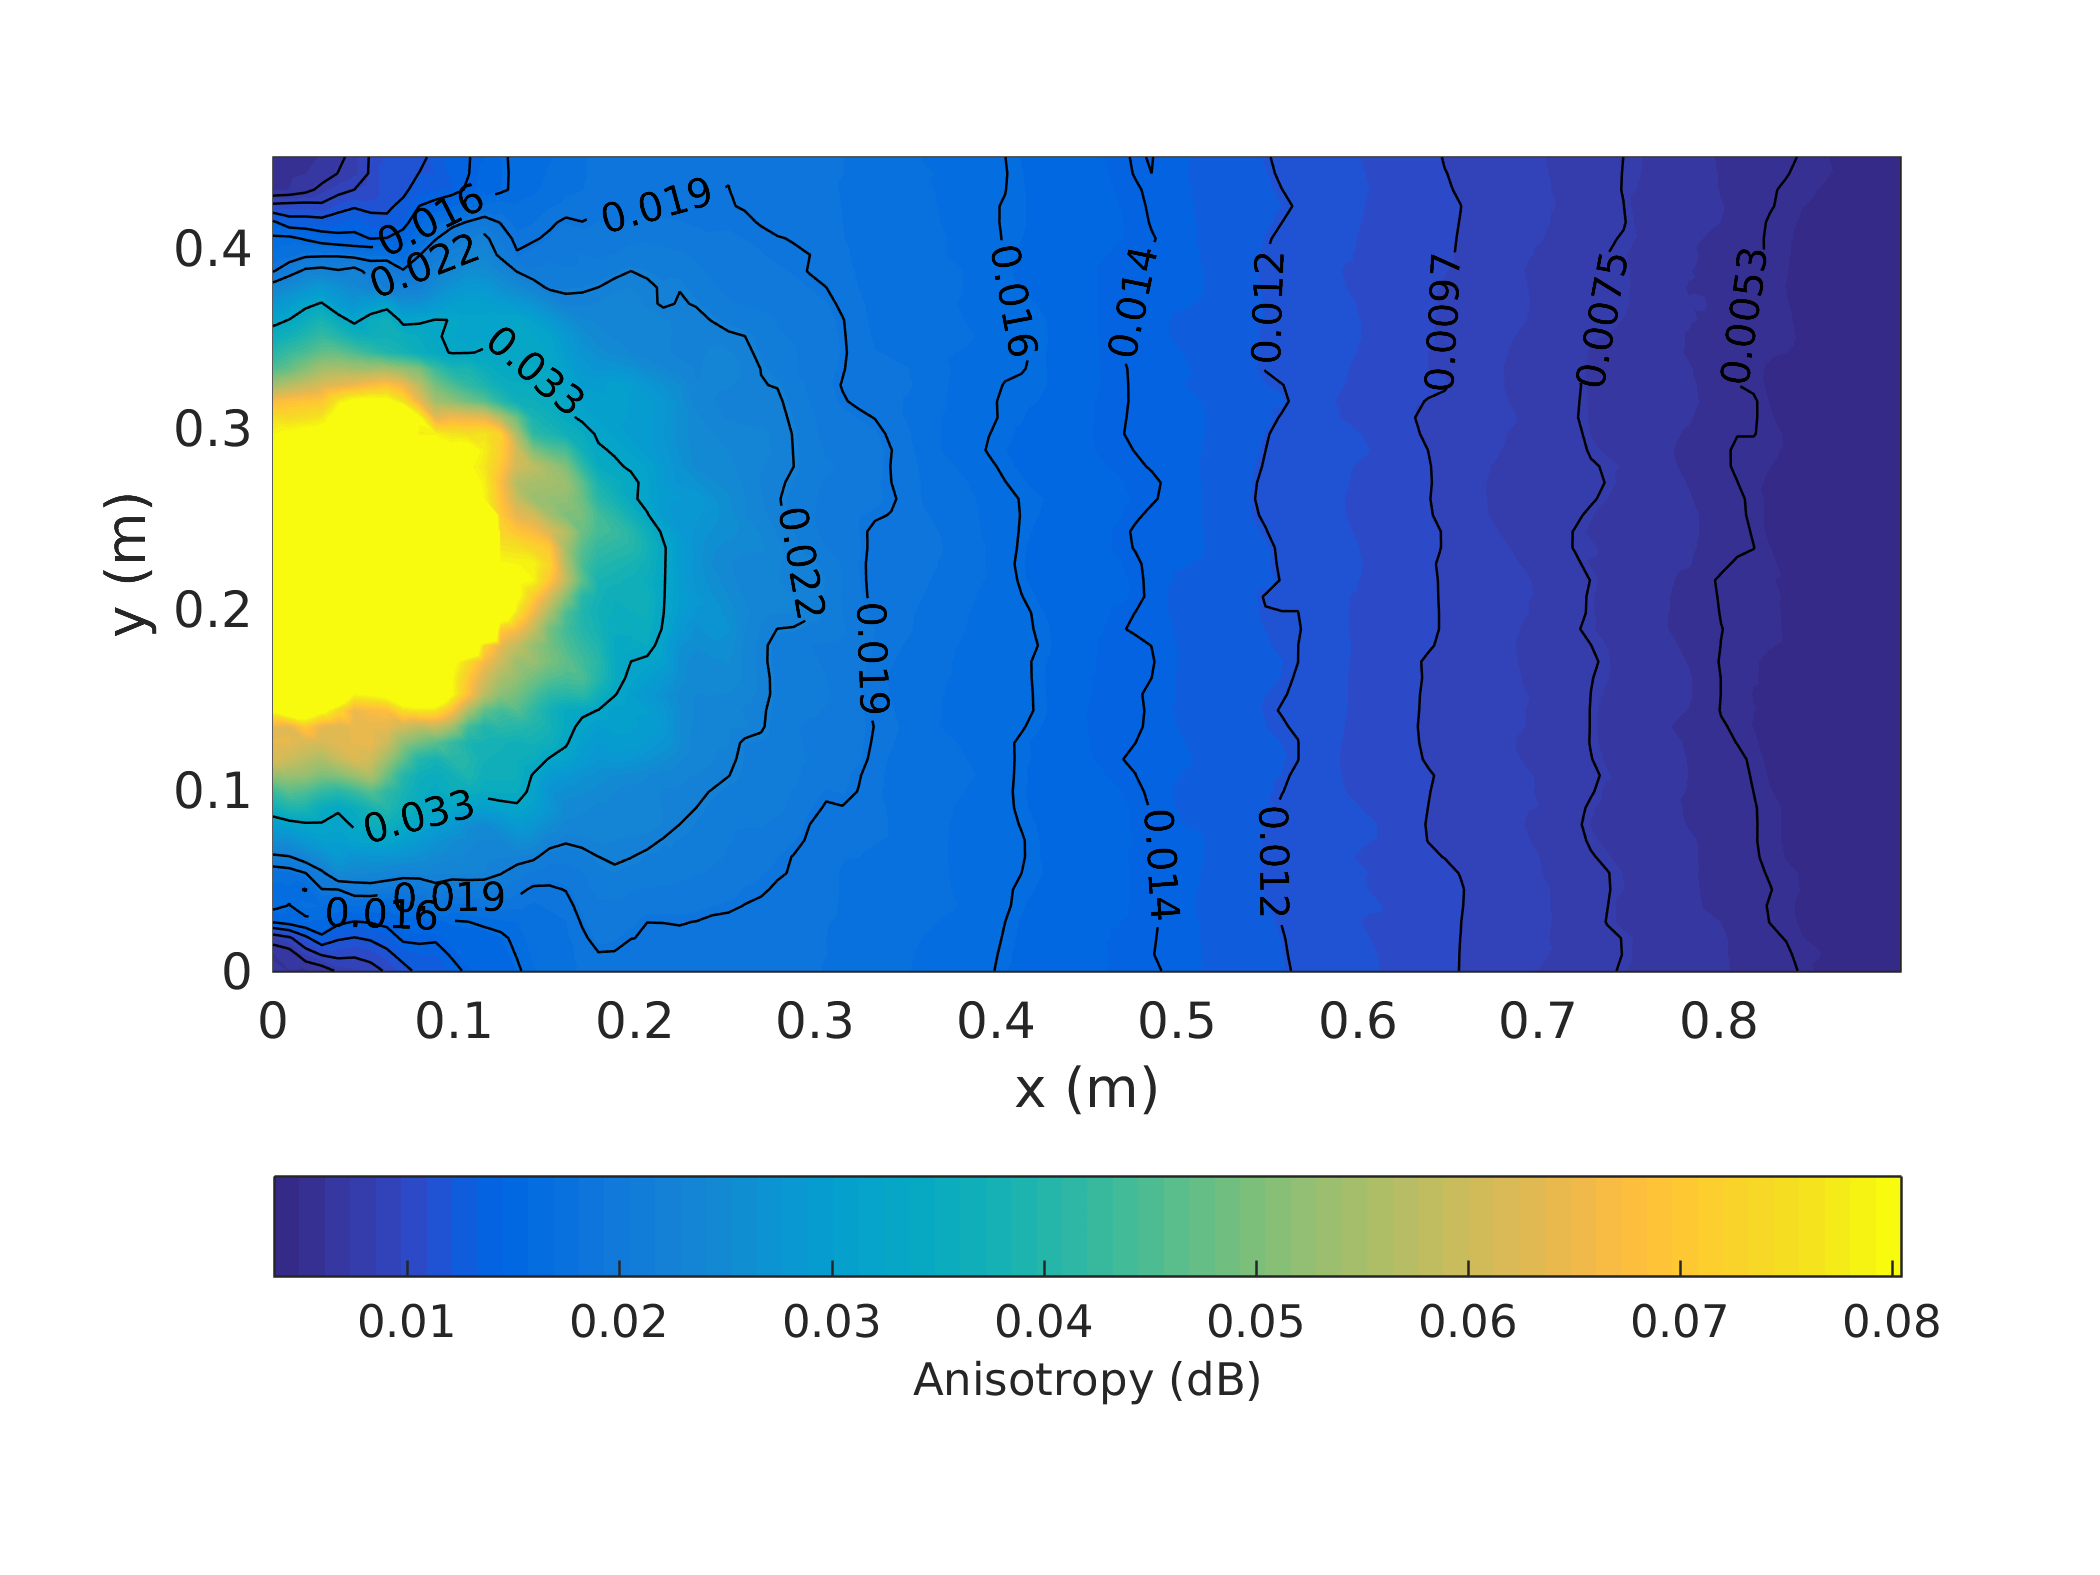
\includegraphics[trim={0 8mm 0 12mm},clip,width=0.52\linewidth]{figures/SDM_3D_SU_EnergyDensityAnisotropyMap}\\
{\footnotesize (c)}\\
\vspace{2mm}
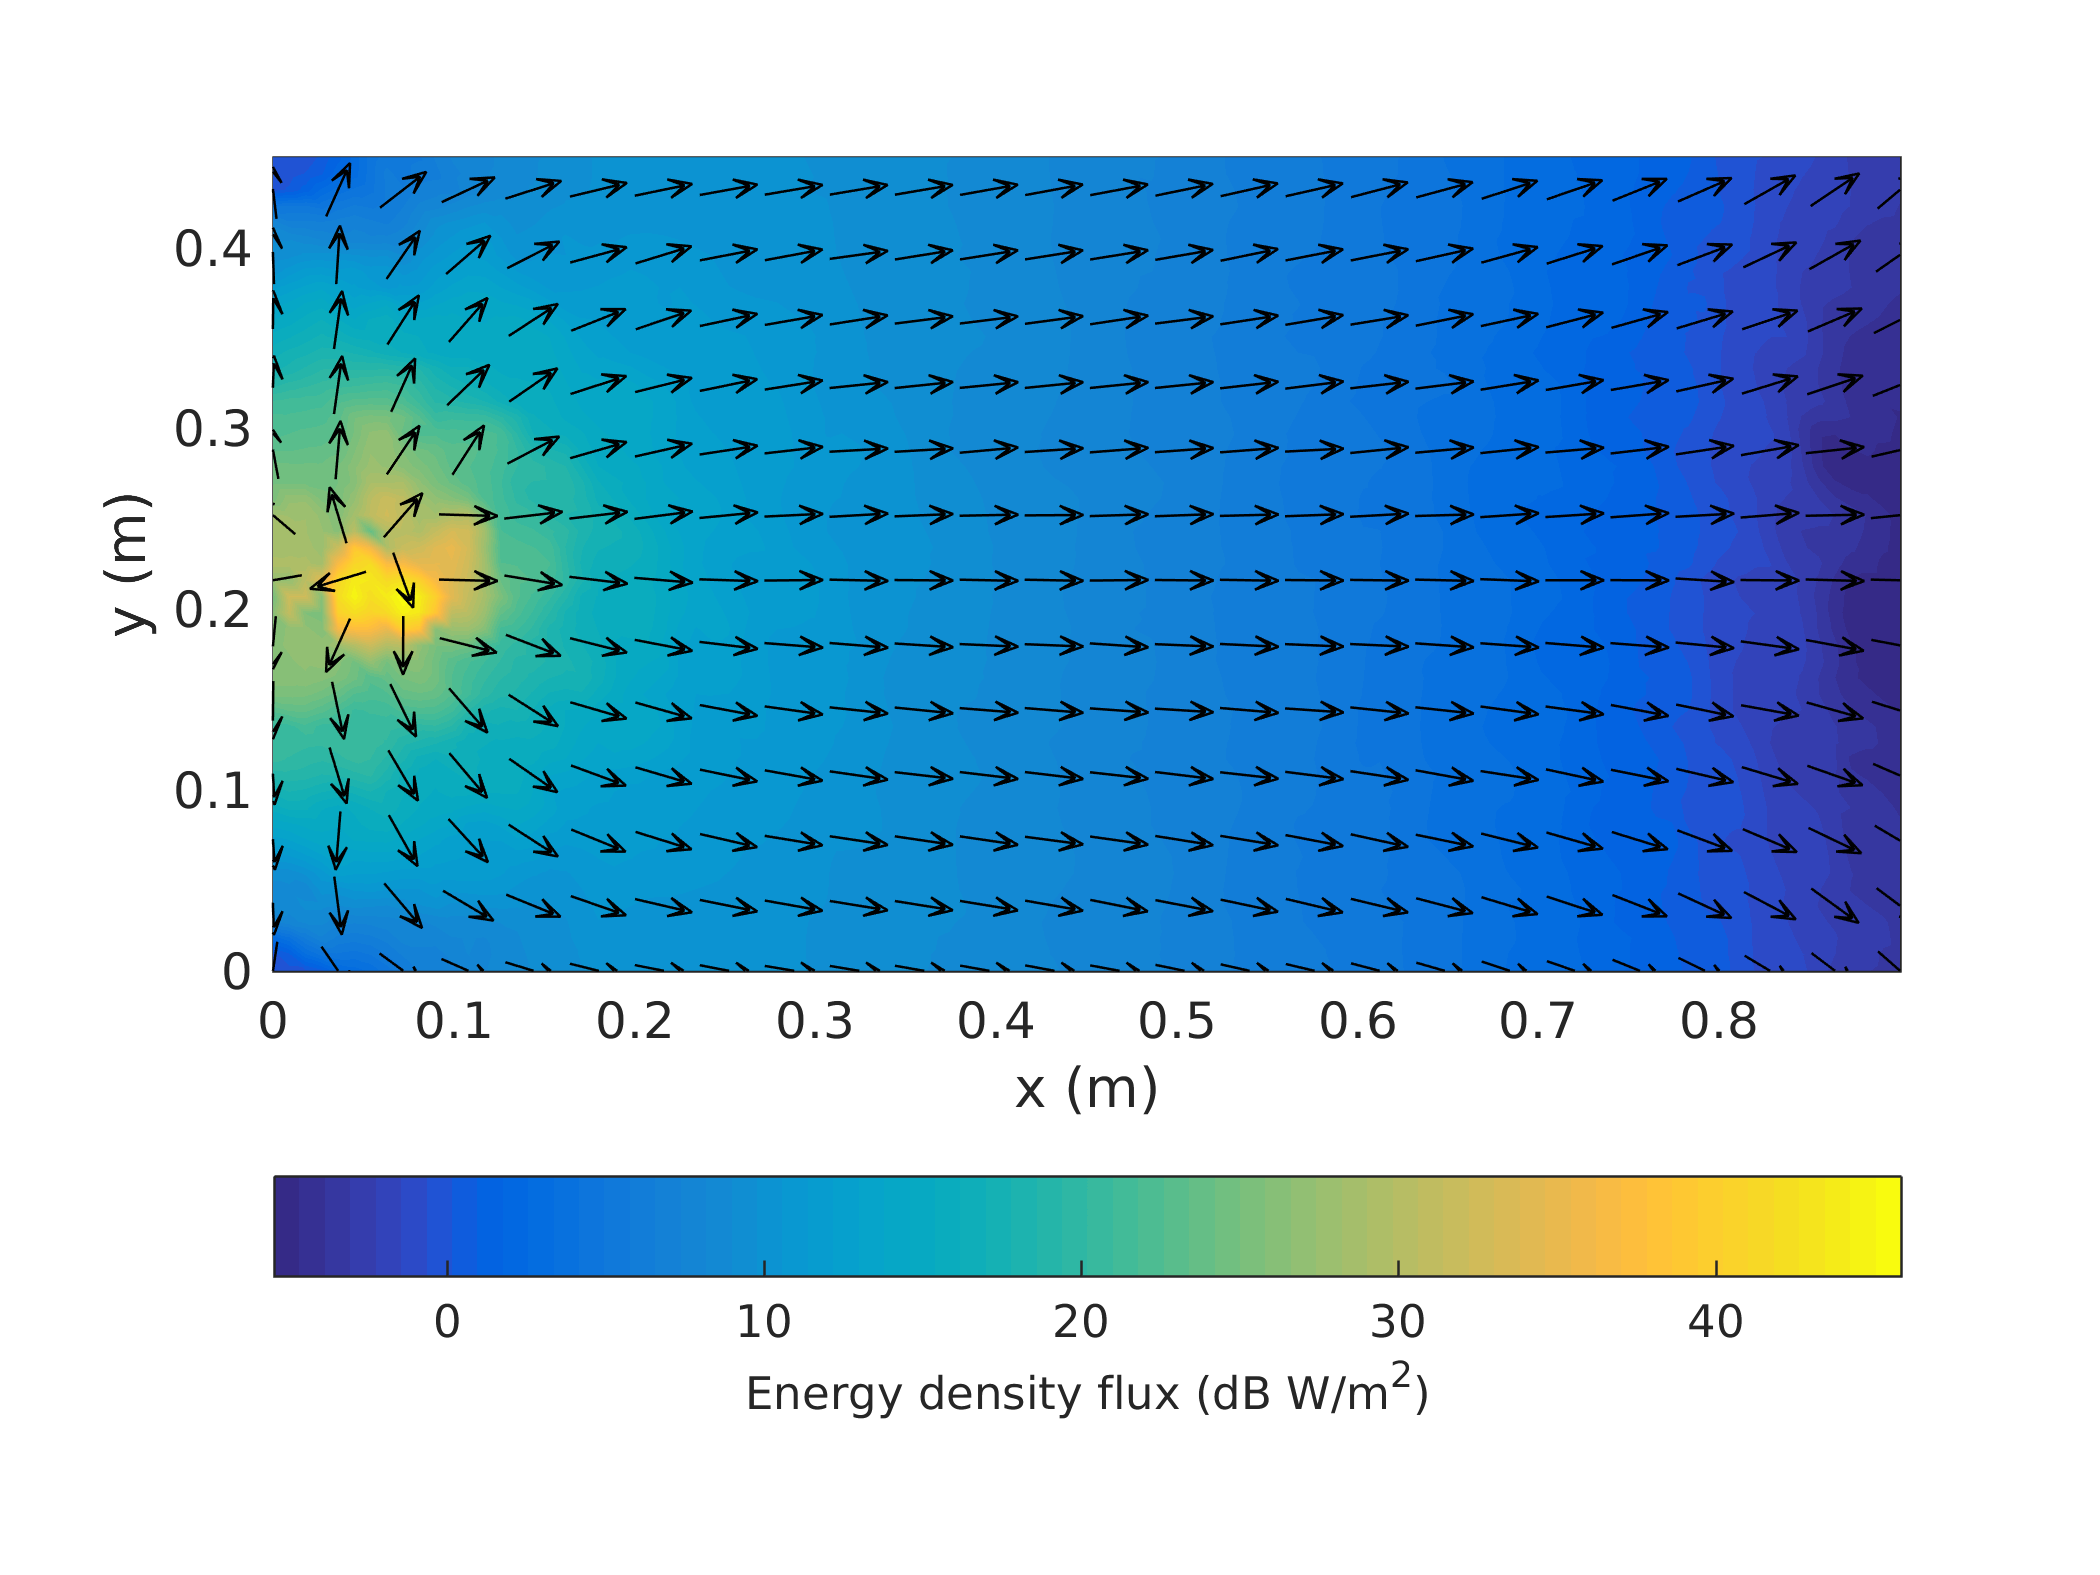
\includegraphics[trim={0 8mm 0 12mm},clip,width=0.52\linewidth]{figures/SDM_3D_SU_EnergyDensityFluxMap}\\
{\footnotesize (d)}\\
\vspace{-2mm}
\caption{\label{fg:unpartempty_maps} 3D EDM maps in the $z$-normal plane at the half height of the cavity for the 
unloaded unpartitioned cavity: (a) Power density; (b) Energy density relative to the homogeneous PWB model;
(c) Anisotropy; (d) Energy density flux.}
\end{center}
\end{figure}

The variation of the power density in the $z$-direction is shown in Figure~\ref{fg:unpartempty_profs}(a)
at $y=L_y/2$ and various values of $x$. In this case the quadratic anzatz used in the Kantorovich reduction
is seen to be quite accurate and the 2D model provides very good results. The variation of the power density 
in the $x$-direction for $z=L_z/2$ and a number of $y$ positions is shown in Figure~\ref{fg:unpartempty_profs}(b).
The power density falls monotonically along the cavity away from the source as expected for a harmonic solution
of the Laplace operator. At the source end of the cavity the EDM predicts higher power density than PWB, while 
at the opposite end the EDM result is lower than the PWB result. The average power density in the EDM in 
Table~\ref{tb:unpartempty} is very close to the PWB prediction. The probability density function (PDF)
for the average power density in the cavity is shown in Figure~\ref{fg:unpartempty_profs}(c); it is a narrow
monomodal distribution.

Figure~\ref{fg:unpartempty_maps} shows maps of various quantities in the $z=L_z/2$ plane. The power density is
shown in Figure~\ref{fg:unpartempty_maps}(a) as a hybrid heat and contour map; the power density is seen to
be relative uniform in the $y$-direction away from the source. The uniformity shown in Figure~\ref{fg:unpartempty_maps}(b)
is the ratio of the EDM and PWB power densities. The zero isoline is located at approximately $x=0.35$, indicating that in 65\,\% of 
the cavity the EDM power density is lower than the PWB power density. The anisotropy of the power density is defined as 
\begin{align}
\Upsilon(\vr) &= \frac{\mathrm{c}_0 w(\vr)}{\mathrm{c}_0 w(\vr) - |\vJ(\vr)|} 
\end{align}
and is shown in Figure~\ref{fg:unpartempty_maps}(c); necessarily it must be greater close to the source. In most of the 
cavity the anisotropy is less than 0.05\,dB. Figure~\ref{fg:unpartempty_maps}(c) shows the flux of the energy density 
as a hybrid heat and vector
field map with the colour indicating the magnitude and the arrow the direction. The flux is again relatively uniform away from 
the source and directed in the positive $x$-direction. 

\subsection[Unpartitioned cavity with a cylinder]{Unpartitioned cavity with a cylinder}
\label{sc:res:unpartcyl}

The derived parameters for the loaded unpartitioned cavity are given in Table~\ref{tb:derivparamsl} and the 
corresponding summary statistics for the average power density in the EDM models are presented 
in Table~\ref{tb:unpartcyl}. Results are given for 2D and 3D SDM cases and also for the 
homogeneous PWB model. The power density varies significantly in the volume of the cavity with a coefficient 
of variation (COV) of about 23,\%. The 2D and 3D EDM are still in close agreement but diverge from the homogeneous
PWB prediction. Even the average EDM power density of 14.3\,dB\,W\,m$^{-2}$ deviates significantly from the PWB value
of 11.9\,dB\,W\,m$^{-2}$. This result was verified using an independently constructed EDM of the specific test-case. 

\begin{table}[ht]
\begin{center}
\begin{tabular}{|c|c|c|}
\hline
\textbf{Parameter}     &\textbf{Unit} &\textbf{Value}\\ 
\hline
\texttt{wallArea}      &m$^2$         &2.0093              \\
\texttt{cavityArea}    &m$^2$         &2.1507              \\
\texttt{cavityVolume}  &m$^3$         &0.17872             \\
\texttt{wallMFP}       &m             &0.35578             \\
\texttt{cylMFP}        &m             &5.0566              \\
\texttt{cavityMFP}     &m             &0.33239             \\
\texttt{wallD}         &m$^2$/s       &3.5553$\times 10^7$ \\
\texttt{cylD}          &m$^2$/s       &5.0531$\times 10^8$ \\
\texttt{cavityD}       &m$^2$/s       &3.3216$\times 10^7$ \\
\texttt{wallACS}       &m$^2$         &0.0013563           \\
\texttt{cavityACS}     &m$^2$         &0.034932            \\
\hline
\end{tabular}
\end{center}
\caption{\label{tb:derivparamsl} Derived parameters for the unpartitioned loaded cavity.}
\end{table}

\begin{table}[ht]
\begin{center}
\begin{tabular}{|l|c|c|c|c|c|}
\hline
\textbf{Power density}               &\textbf{PWB} &\multicolumn{2}{|c|}{\textbf{EDM}} \\ \cline{3-4}
{}                                   &{}           &\textbf{2D SDM} &\textbf{3D SDM}  \\
\hline
Value at centre (dB\,W\,m$^{-2})$    &14.57        &15.90           &15.85 \\
Mean (dB\,W\,m$^{-2})$               &14.57        &16.00           &15.93 \\
Minimum (dB\,W\,m$^{-2})$            &14.57        &14.12           &12.69 \\
Maximum (dB\,W\,m$^{-2})$            &14.57        &17.72           &18.12 \\
Standard deviation (dB\,W\,m$^{-2})$ &0            &9.54            &9.37  \\
Coefficient of variation (\%)        &0            &22.6            &22.1  \\
\hline
\end{tabular}
\end{center}
\caption{\label{tb:unpartcyl} Statistics of the reverberant power density in the unpartitioned cavity with the cylinder.}
\end{table}

\begin{figure}[hp]
\begin{center}
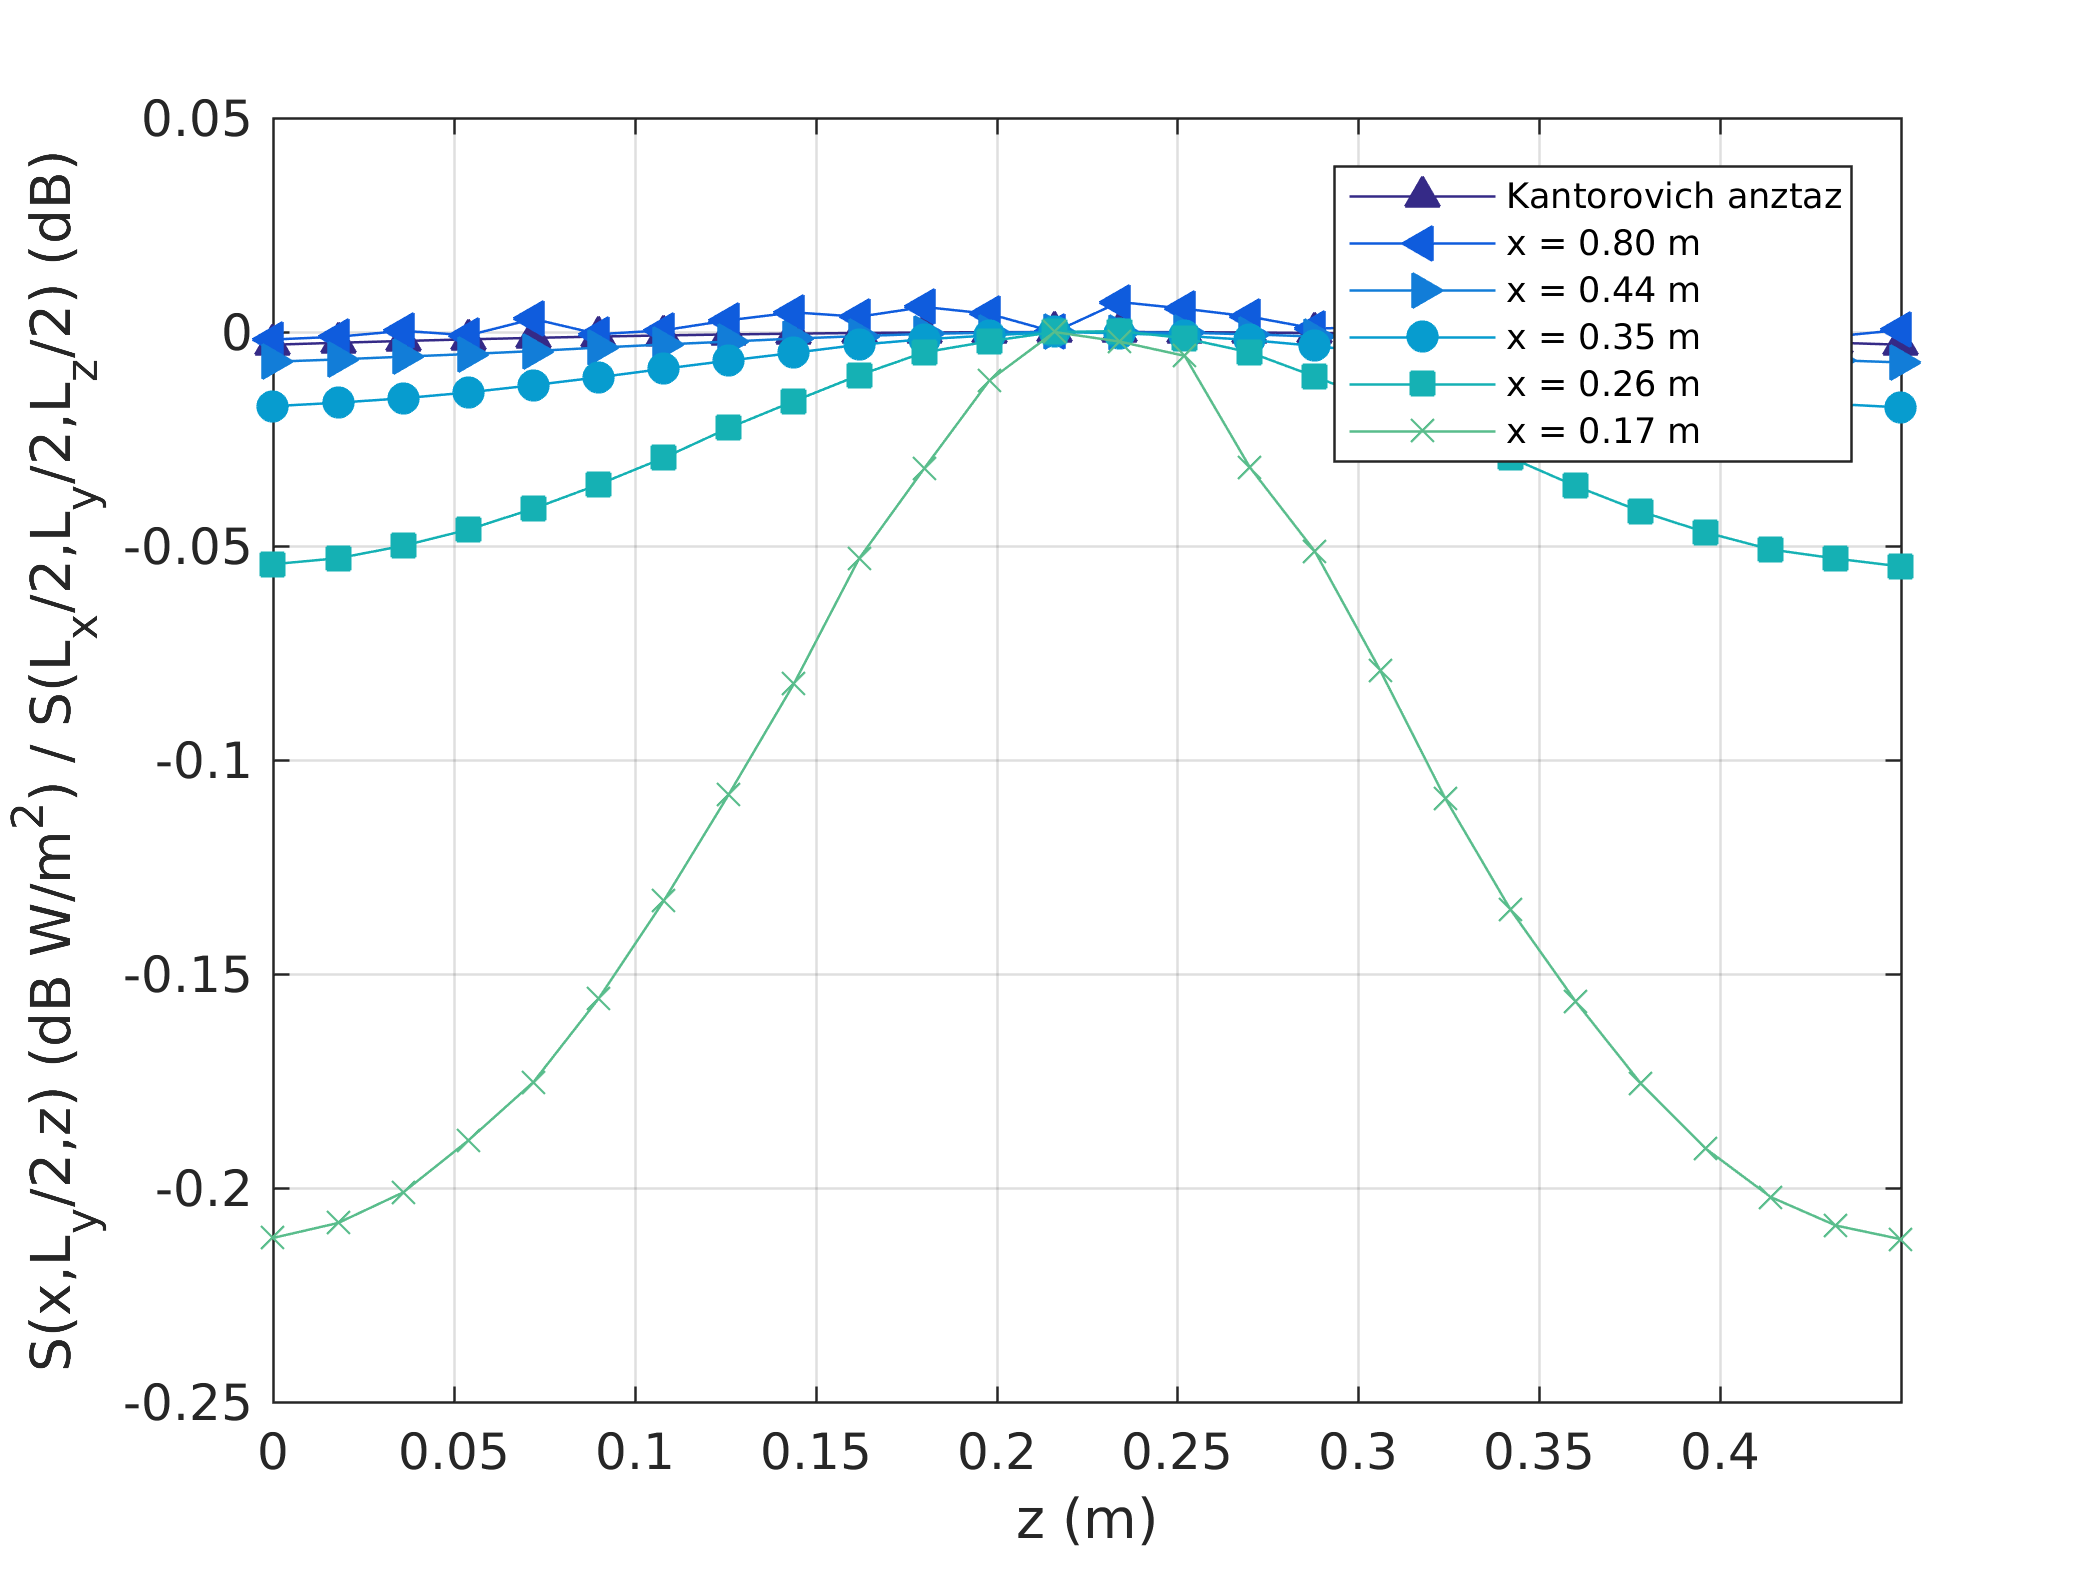
\includegraphics[width=0.6\linewidth]{figures/SDM_3D_SL_PowerDensityProfileZ}\\
{\footnotesize (a)}\\
\vspace{2mm}
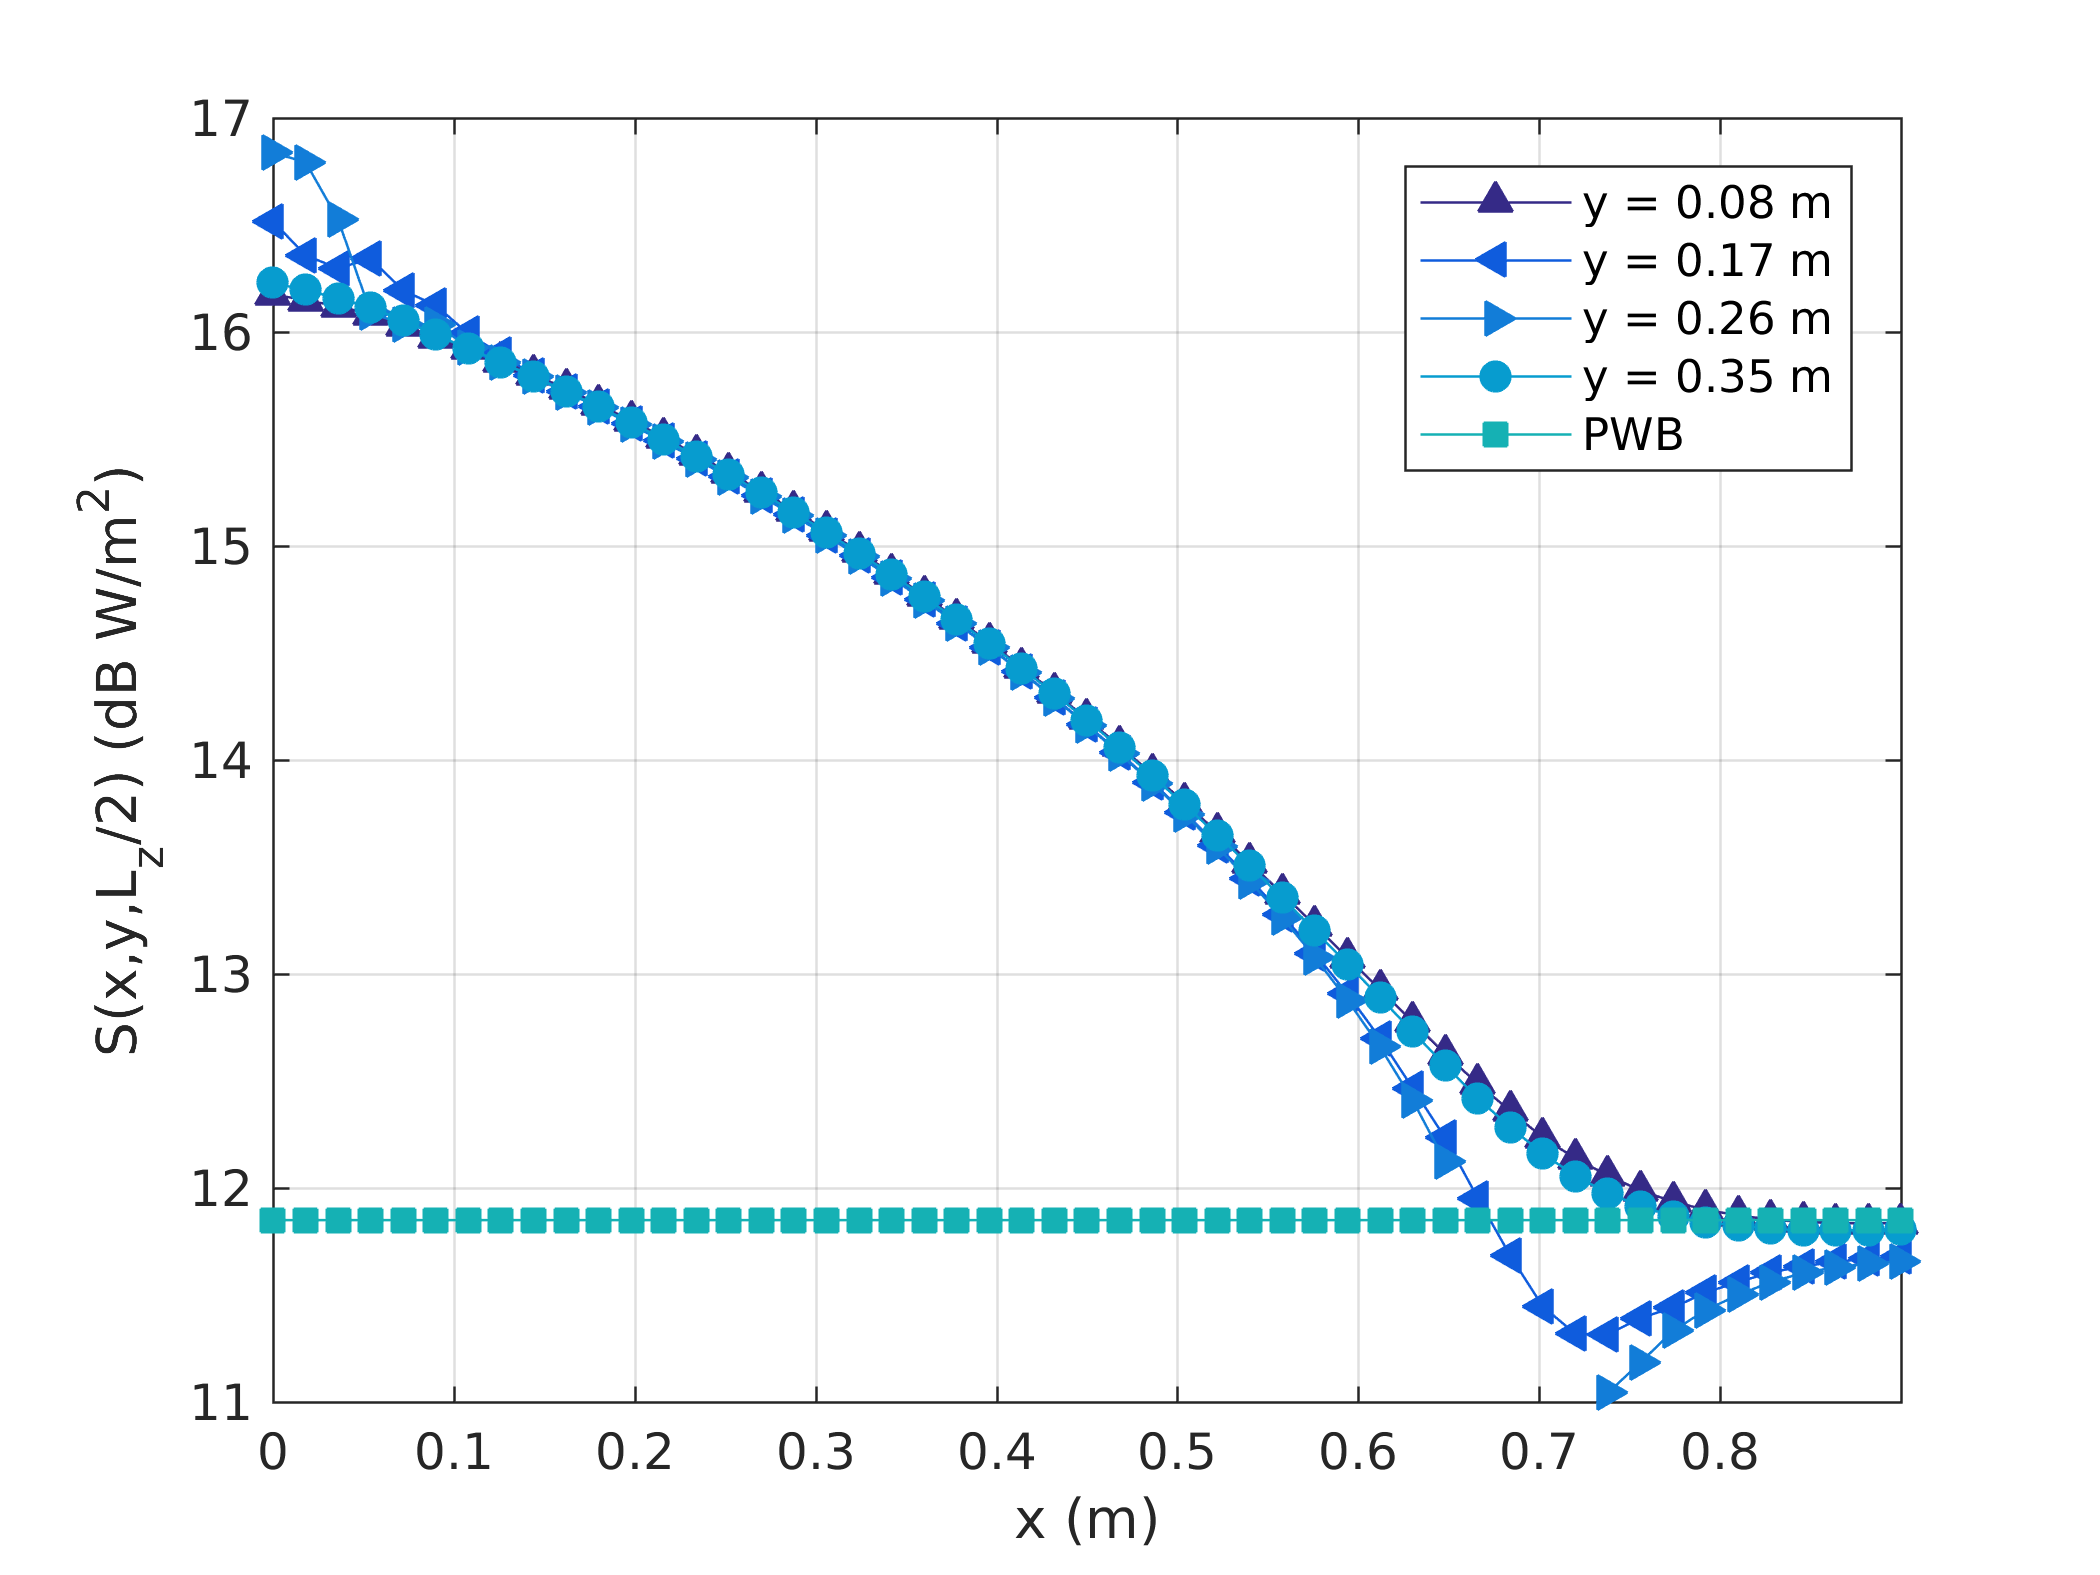
\includegraphics[width=0.6\linewidth]{figures/SDM_3D_SL_PowerDensityProfileX}\\
{\footnotesize (b)}\\
\vspace{2mm}
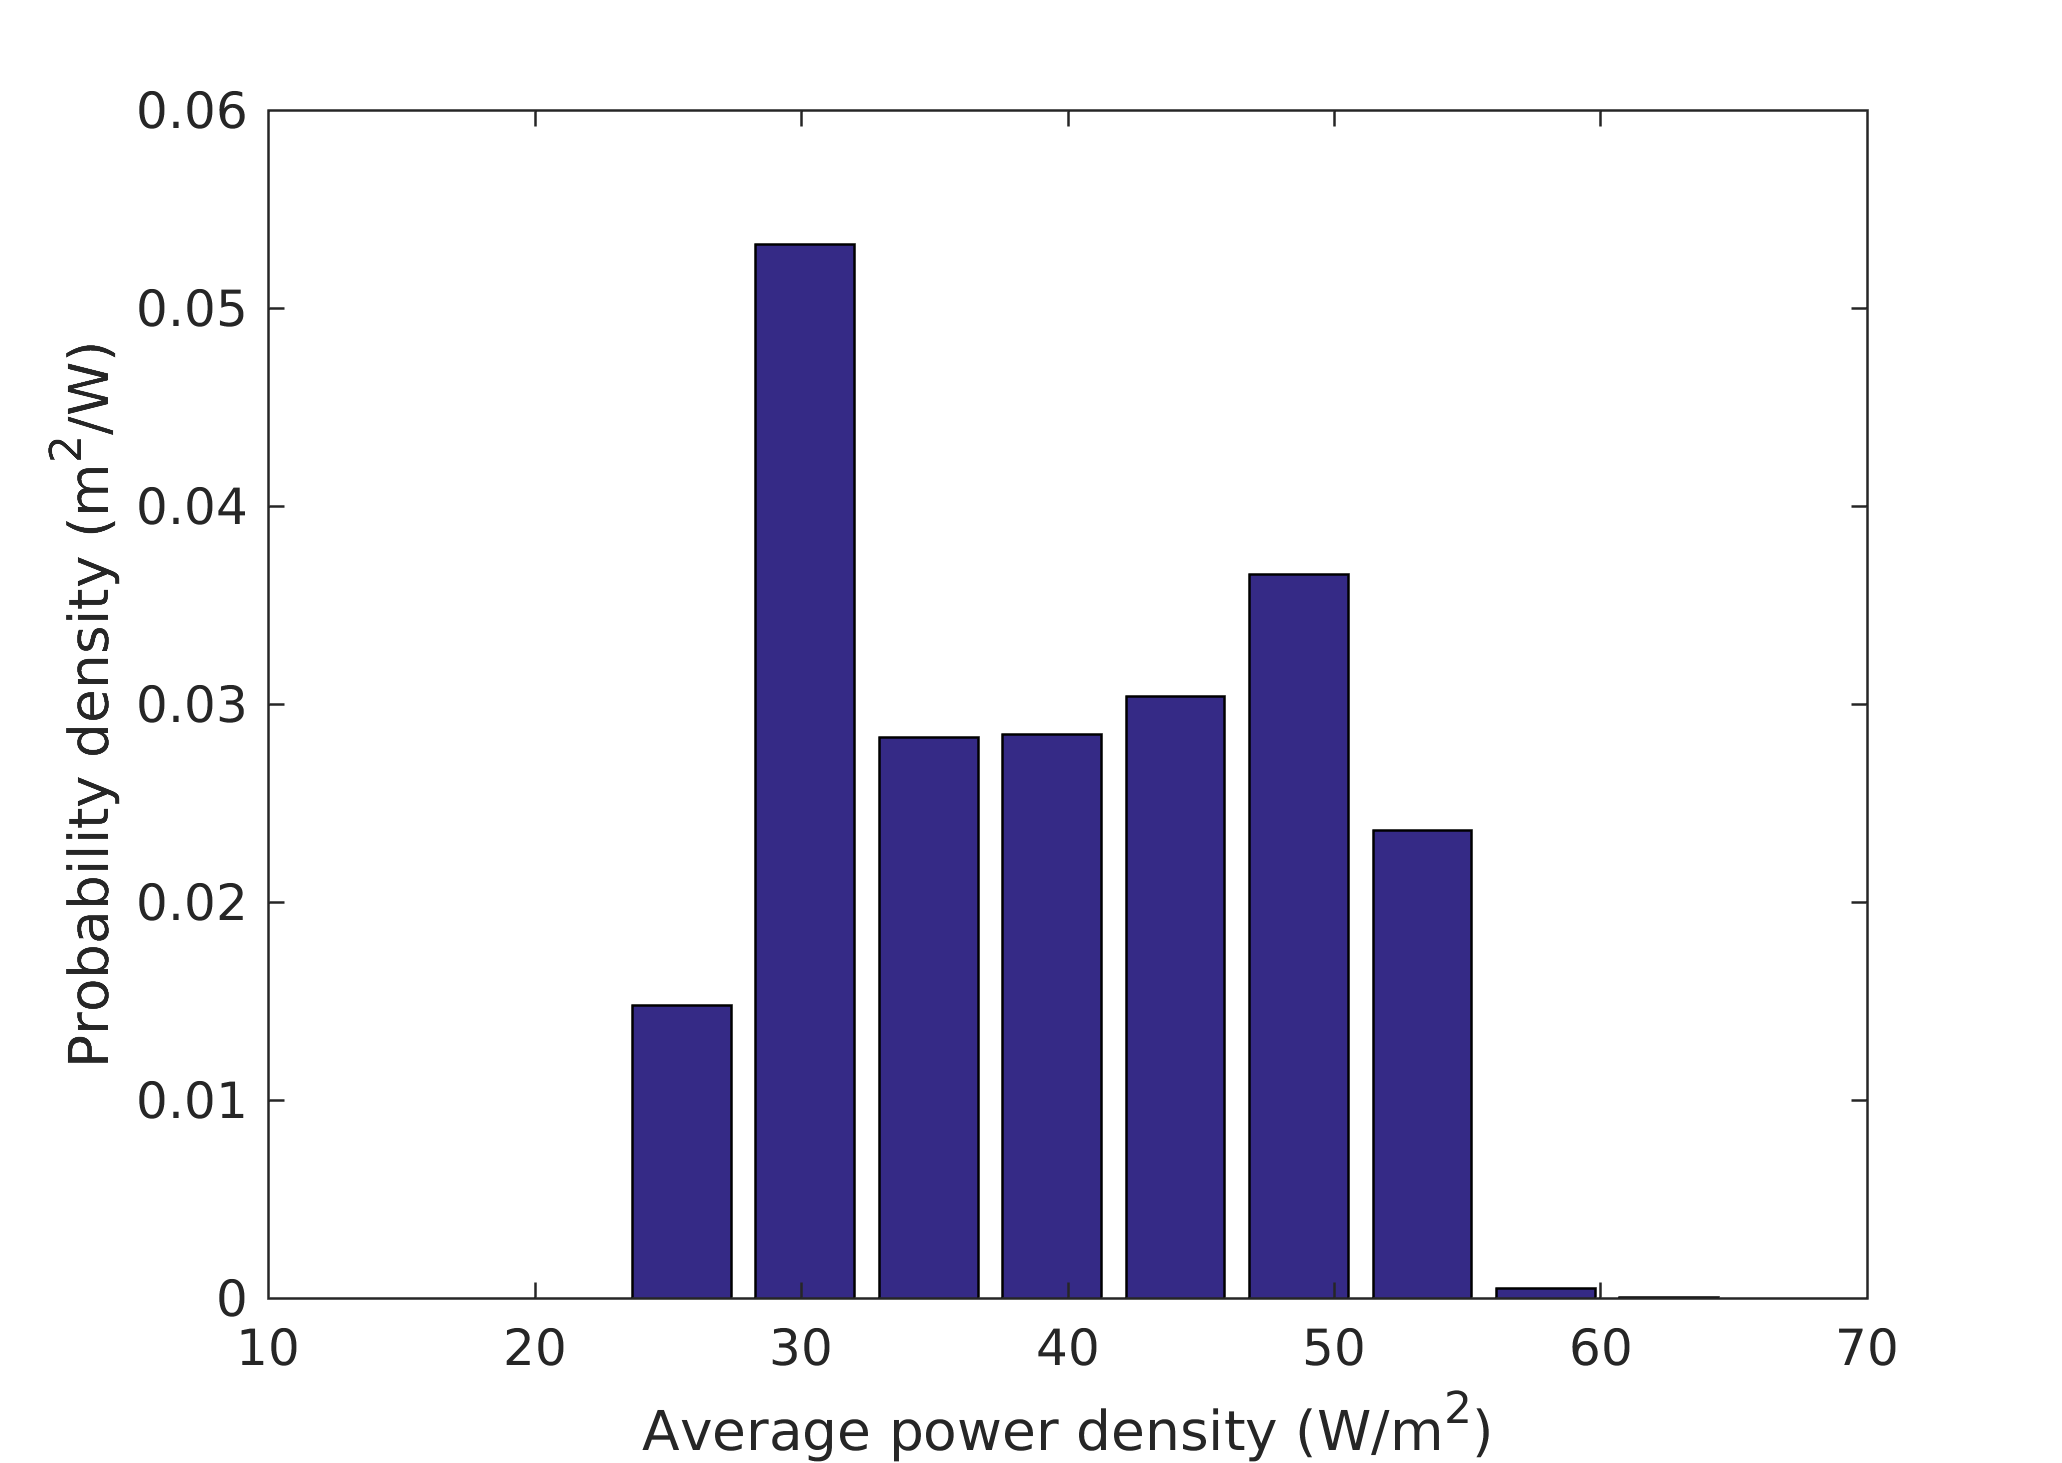
\includegraphics[width=0.6\linewidth]{figures/SDM_3D_SL_PowerDensityPDF}\\
{\footnotesize (c)}\\
\vspace{-2mm}
\caption{\label{fg:unpartcyl_profs} EDM of the loaded unpartitioned cavity: (a) Normalised vertical profile of the power density; 
(b) Power density profile in the $x$-direction along the cavity centre; (c) PDF of the power density throughout the cavity volume.}
\end{center}
\end{figure}

\begin{figure}[hp]
\begin{center}
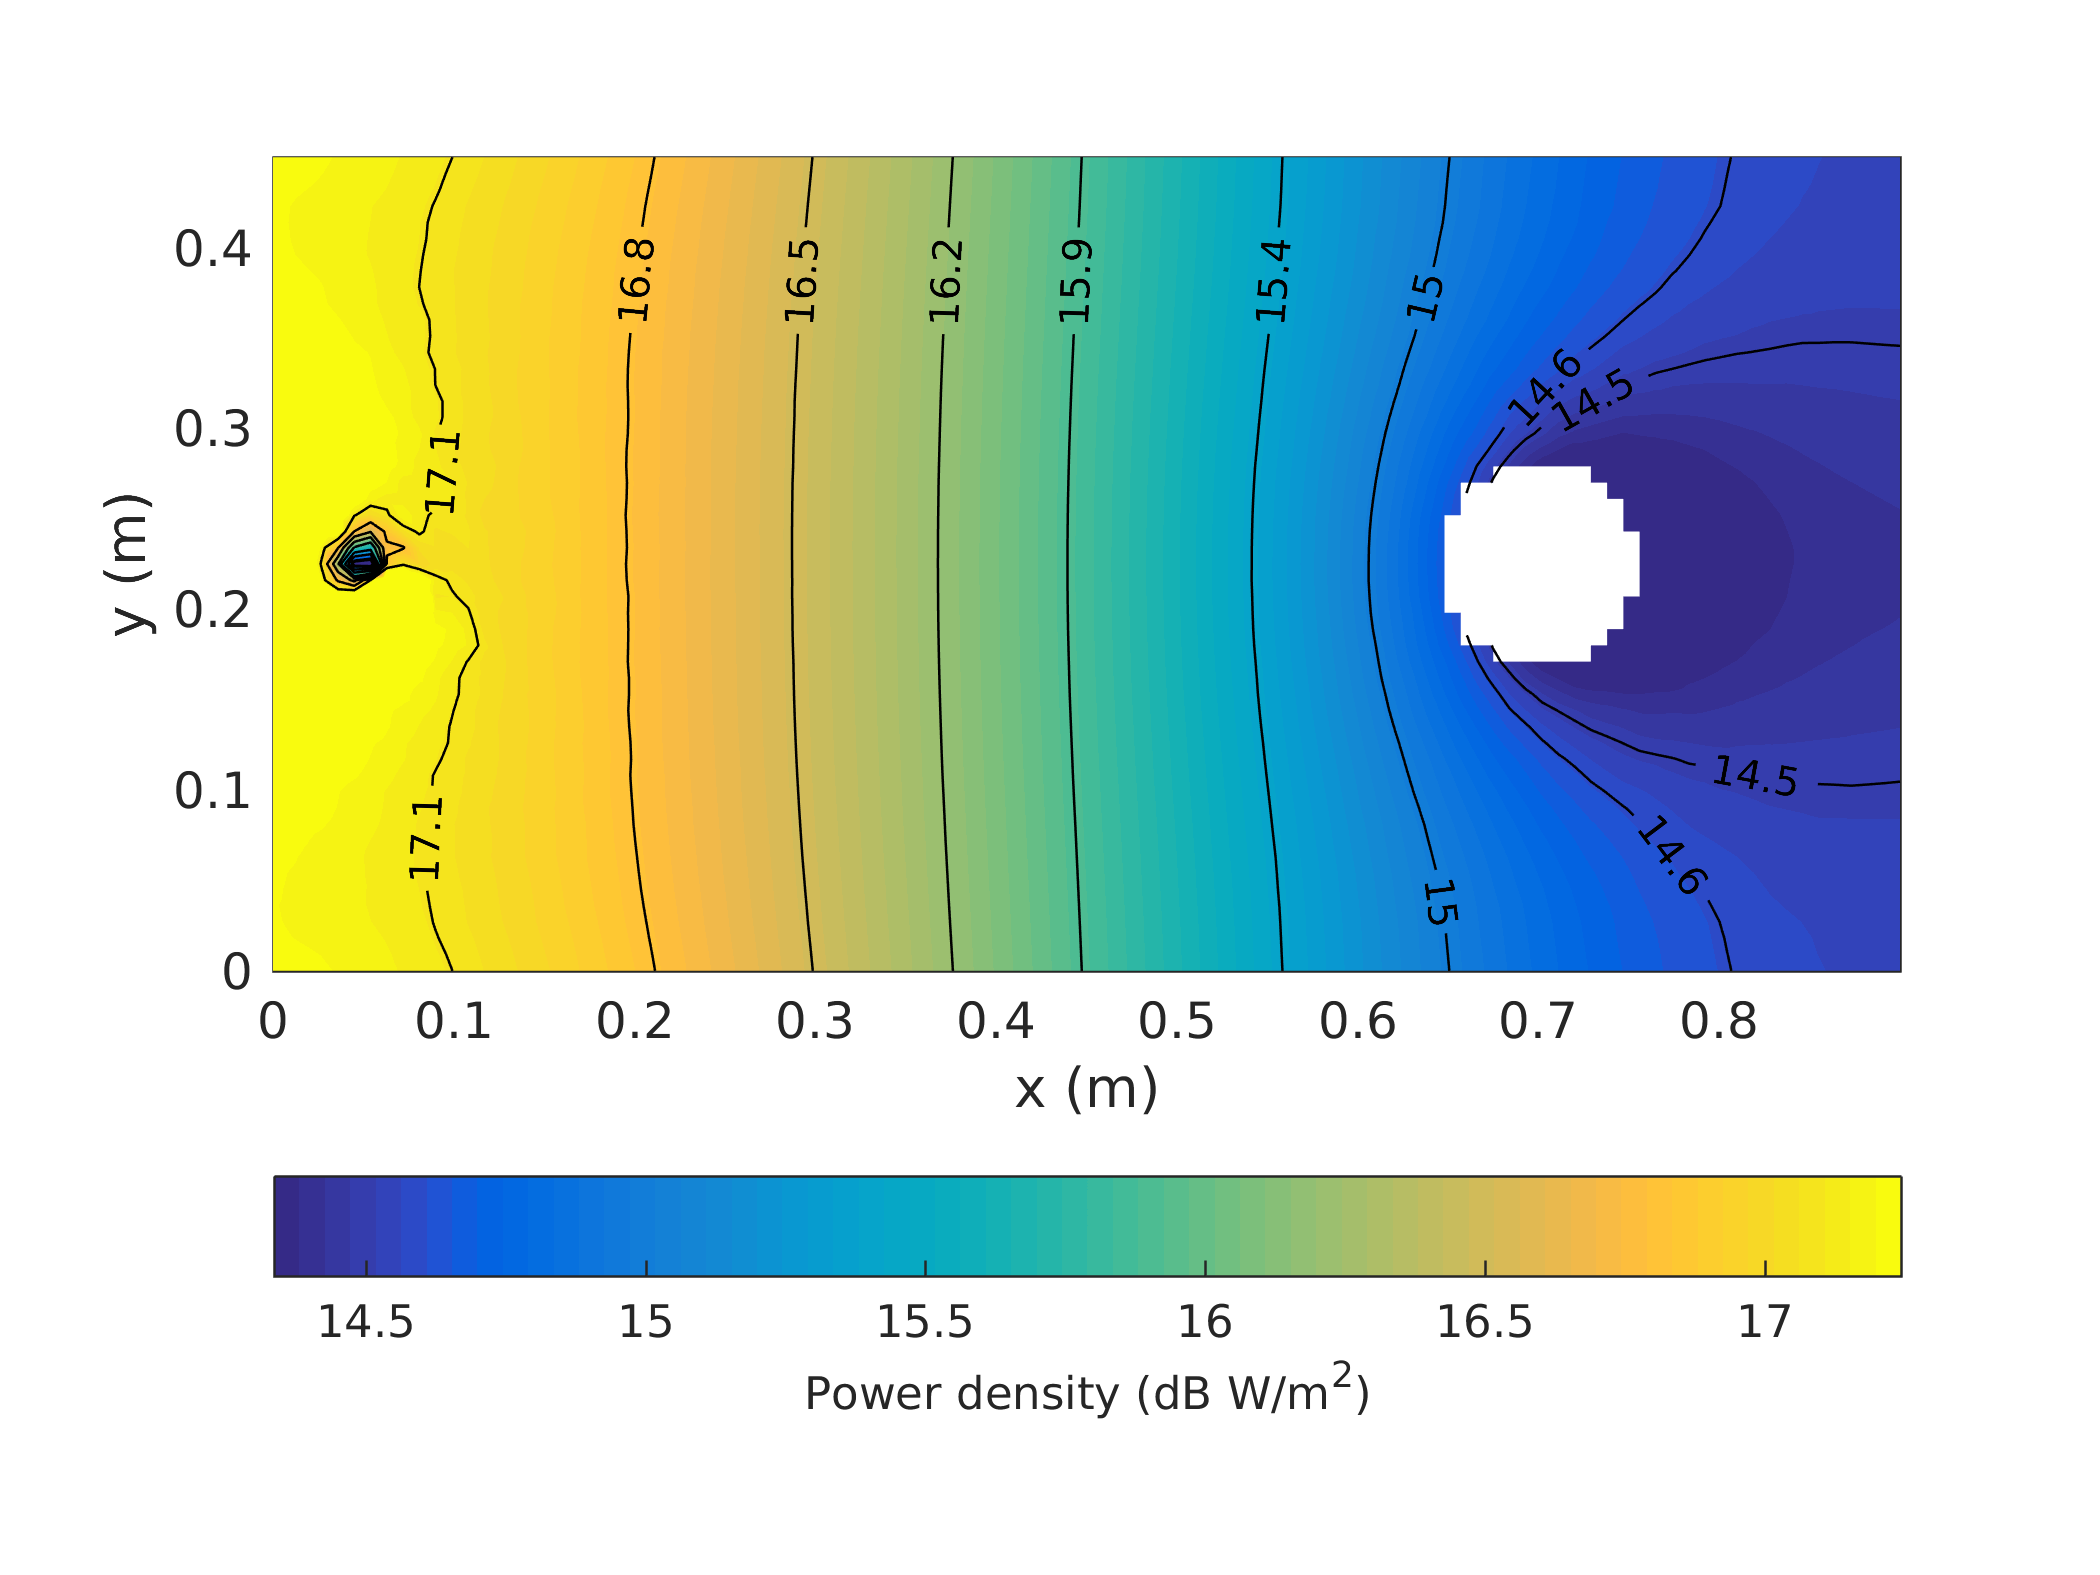
\includegraphics[trim={0 8mm 0 12mm},clip,width=0.52\linewidth]{figures/SDM_3D_SL_PowerDensityMap}\\
{\footnotesize (a)}\\
\vspace{2mm}
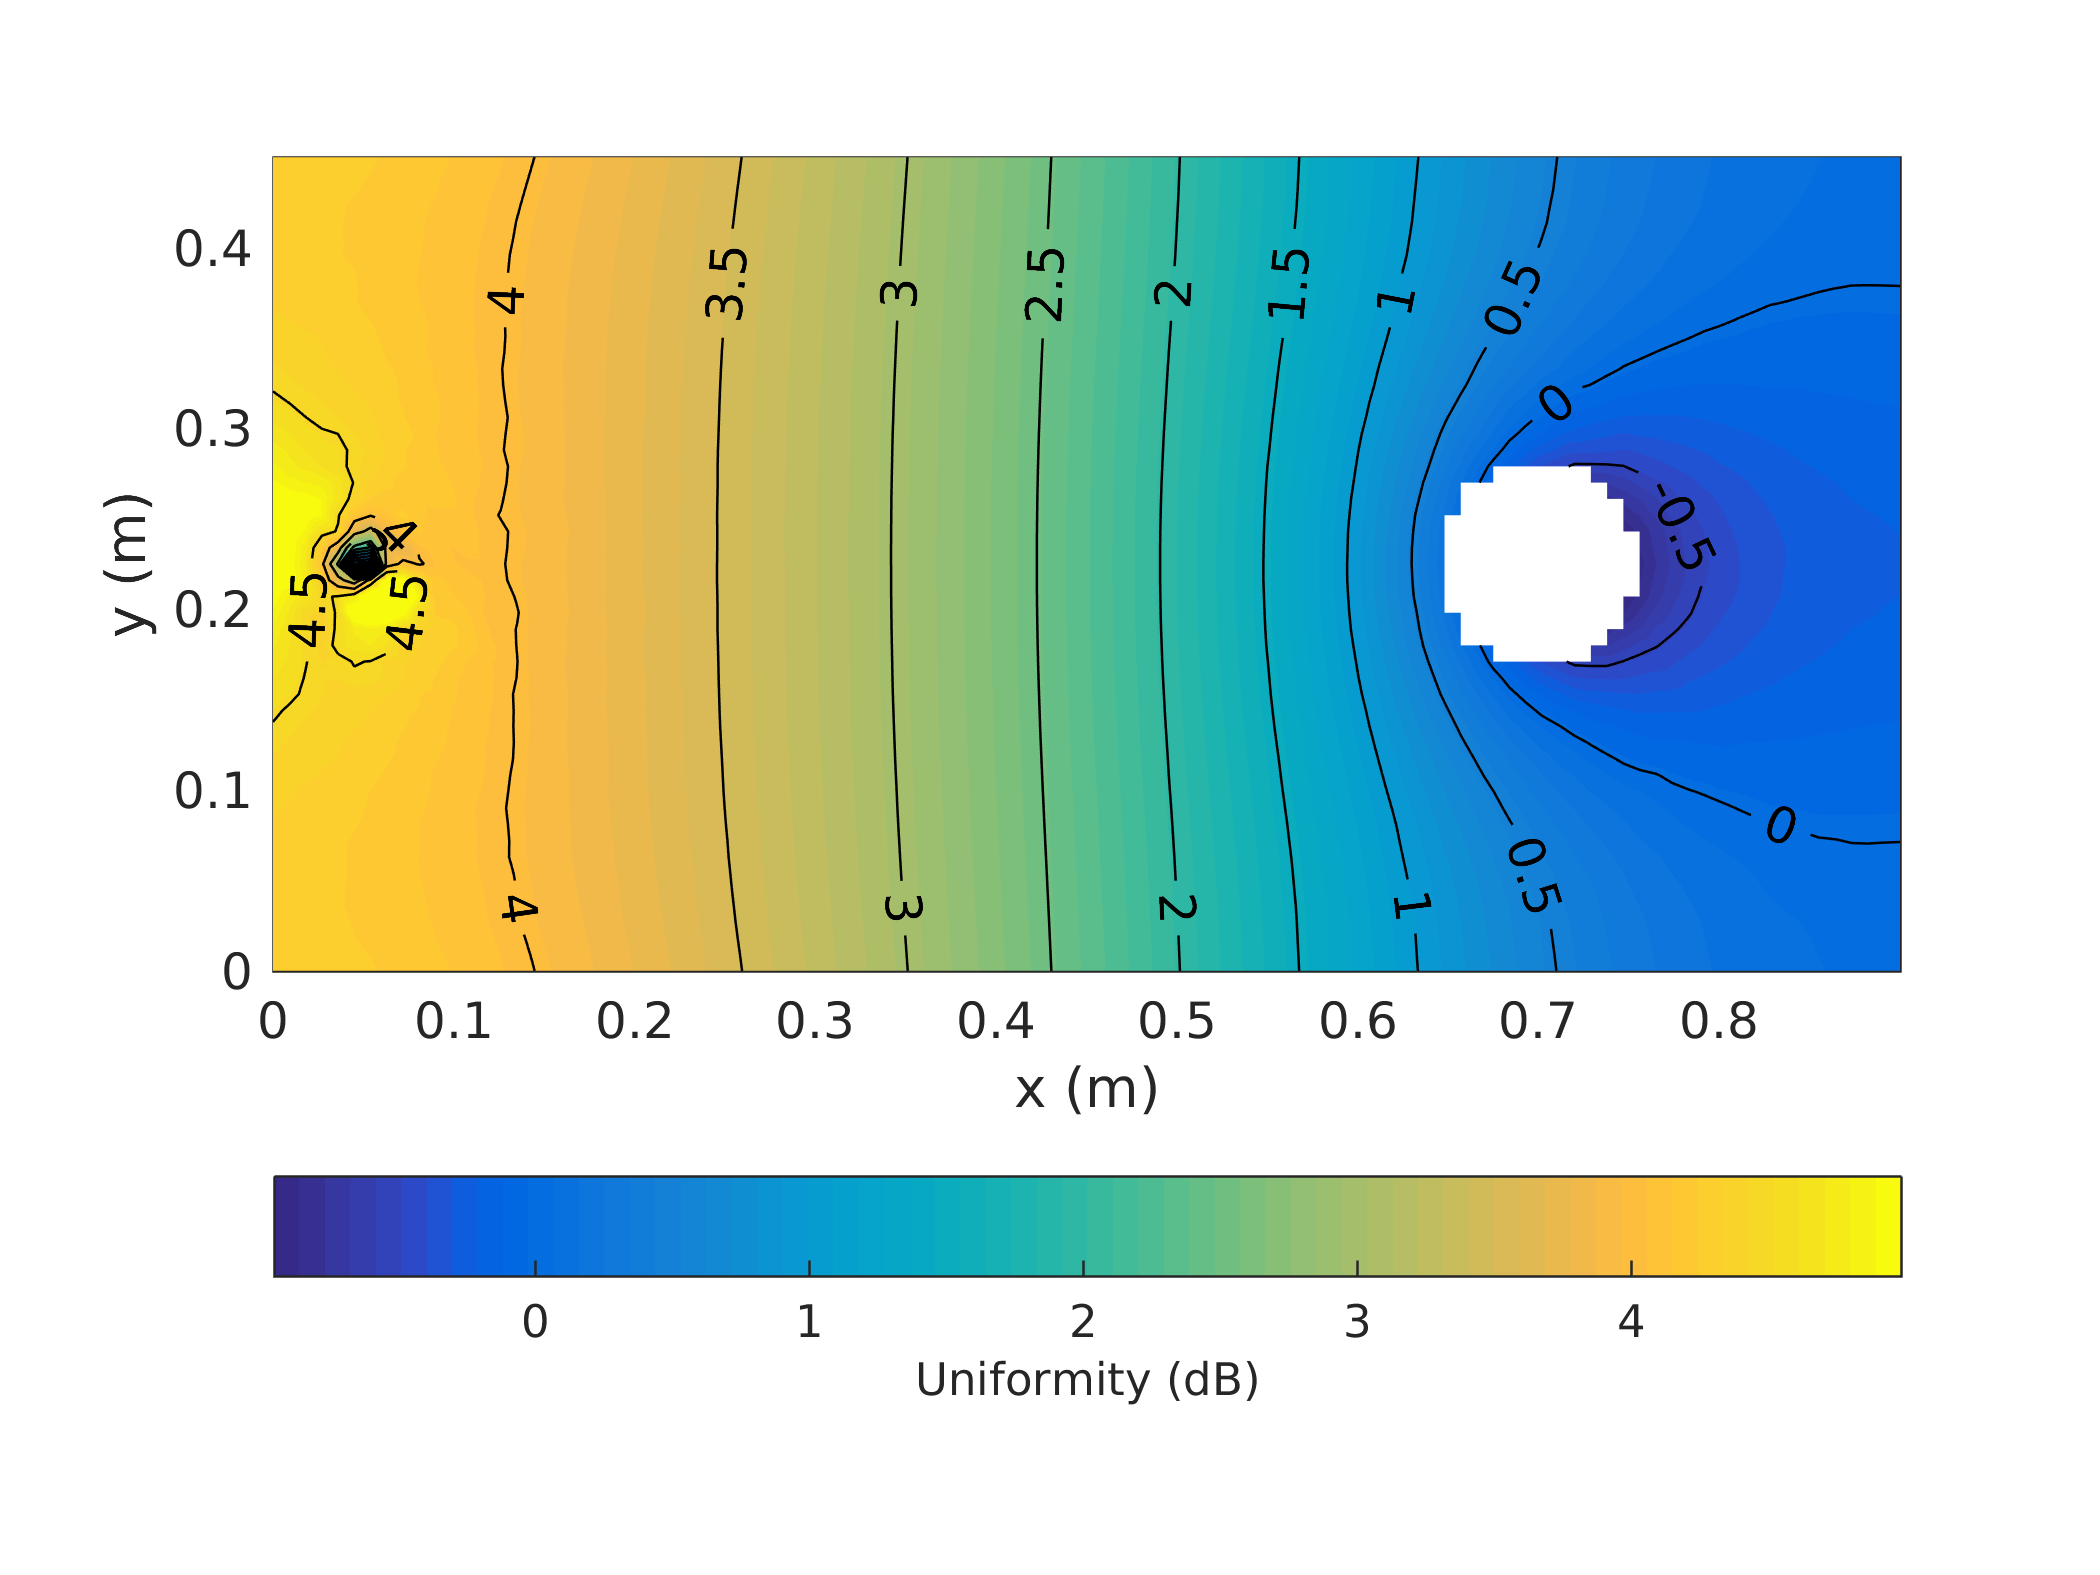
\includegraphics[trim={0 8mm 0 12mm},clip,width=0.52\linewidth]{figures/SDM_3D_SL_EnergyDensityUniformityMap}\\
{\footnotesize (b)}\\
\vspace{2mm}
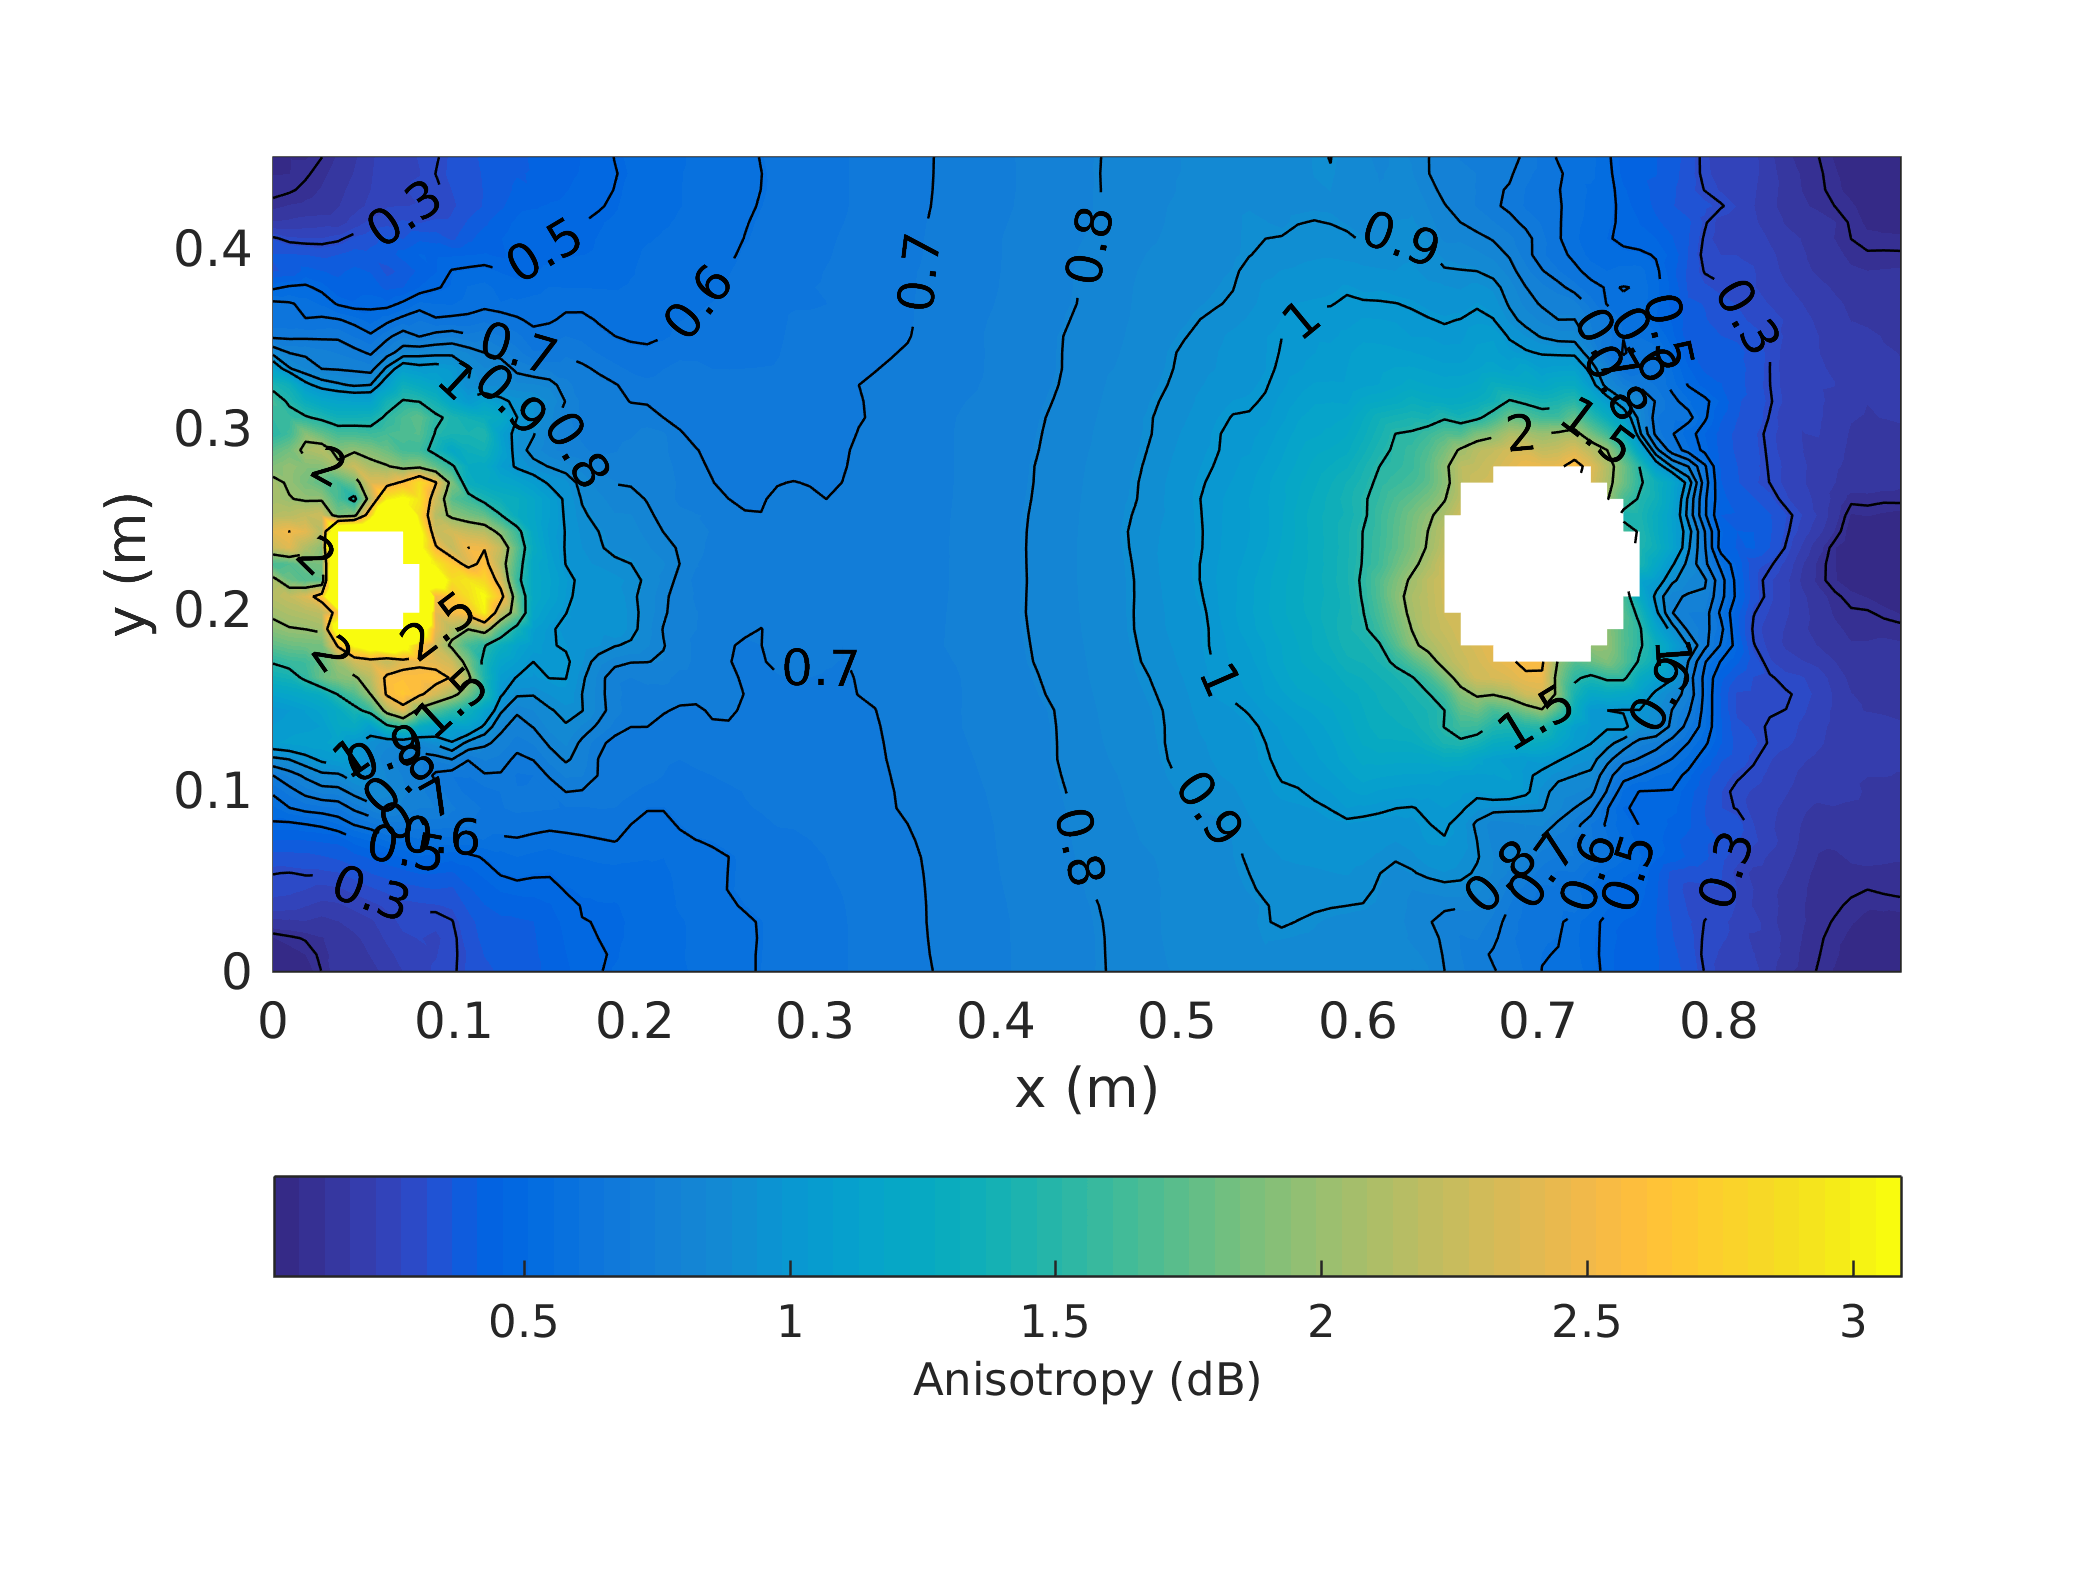
\includegraphics[trim={0 8mm 0 12mm},clip,width=0.52\linewidth]{figures/SDM_3D_SL_EnergyDensityAnisotropyMap}\\
{\footnotesize (c)}\\
\vspace{2mm}
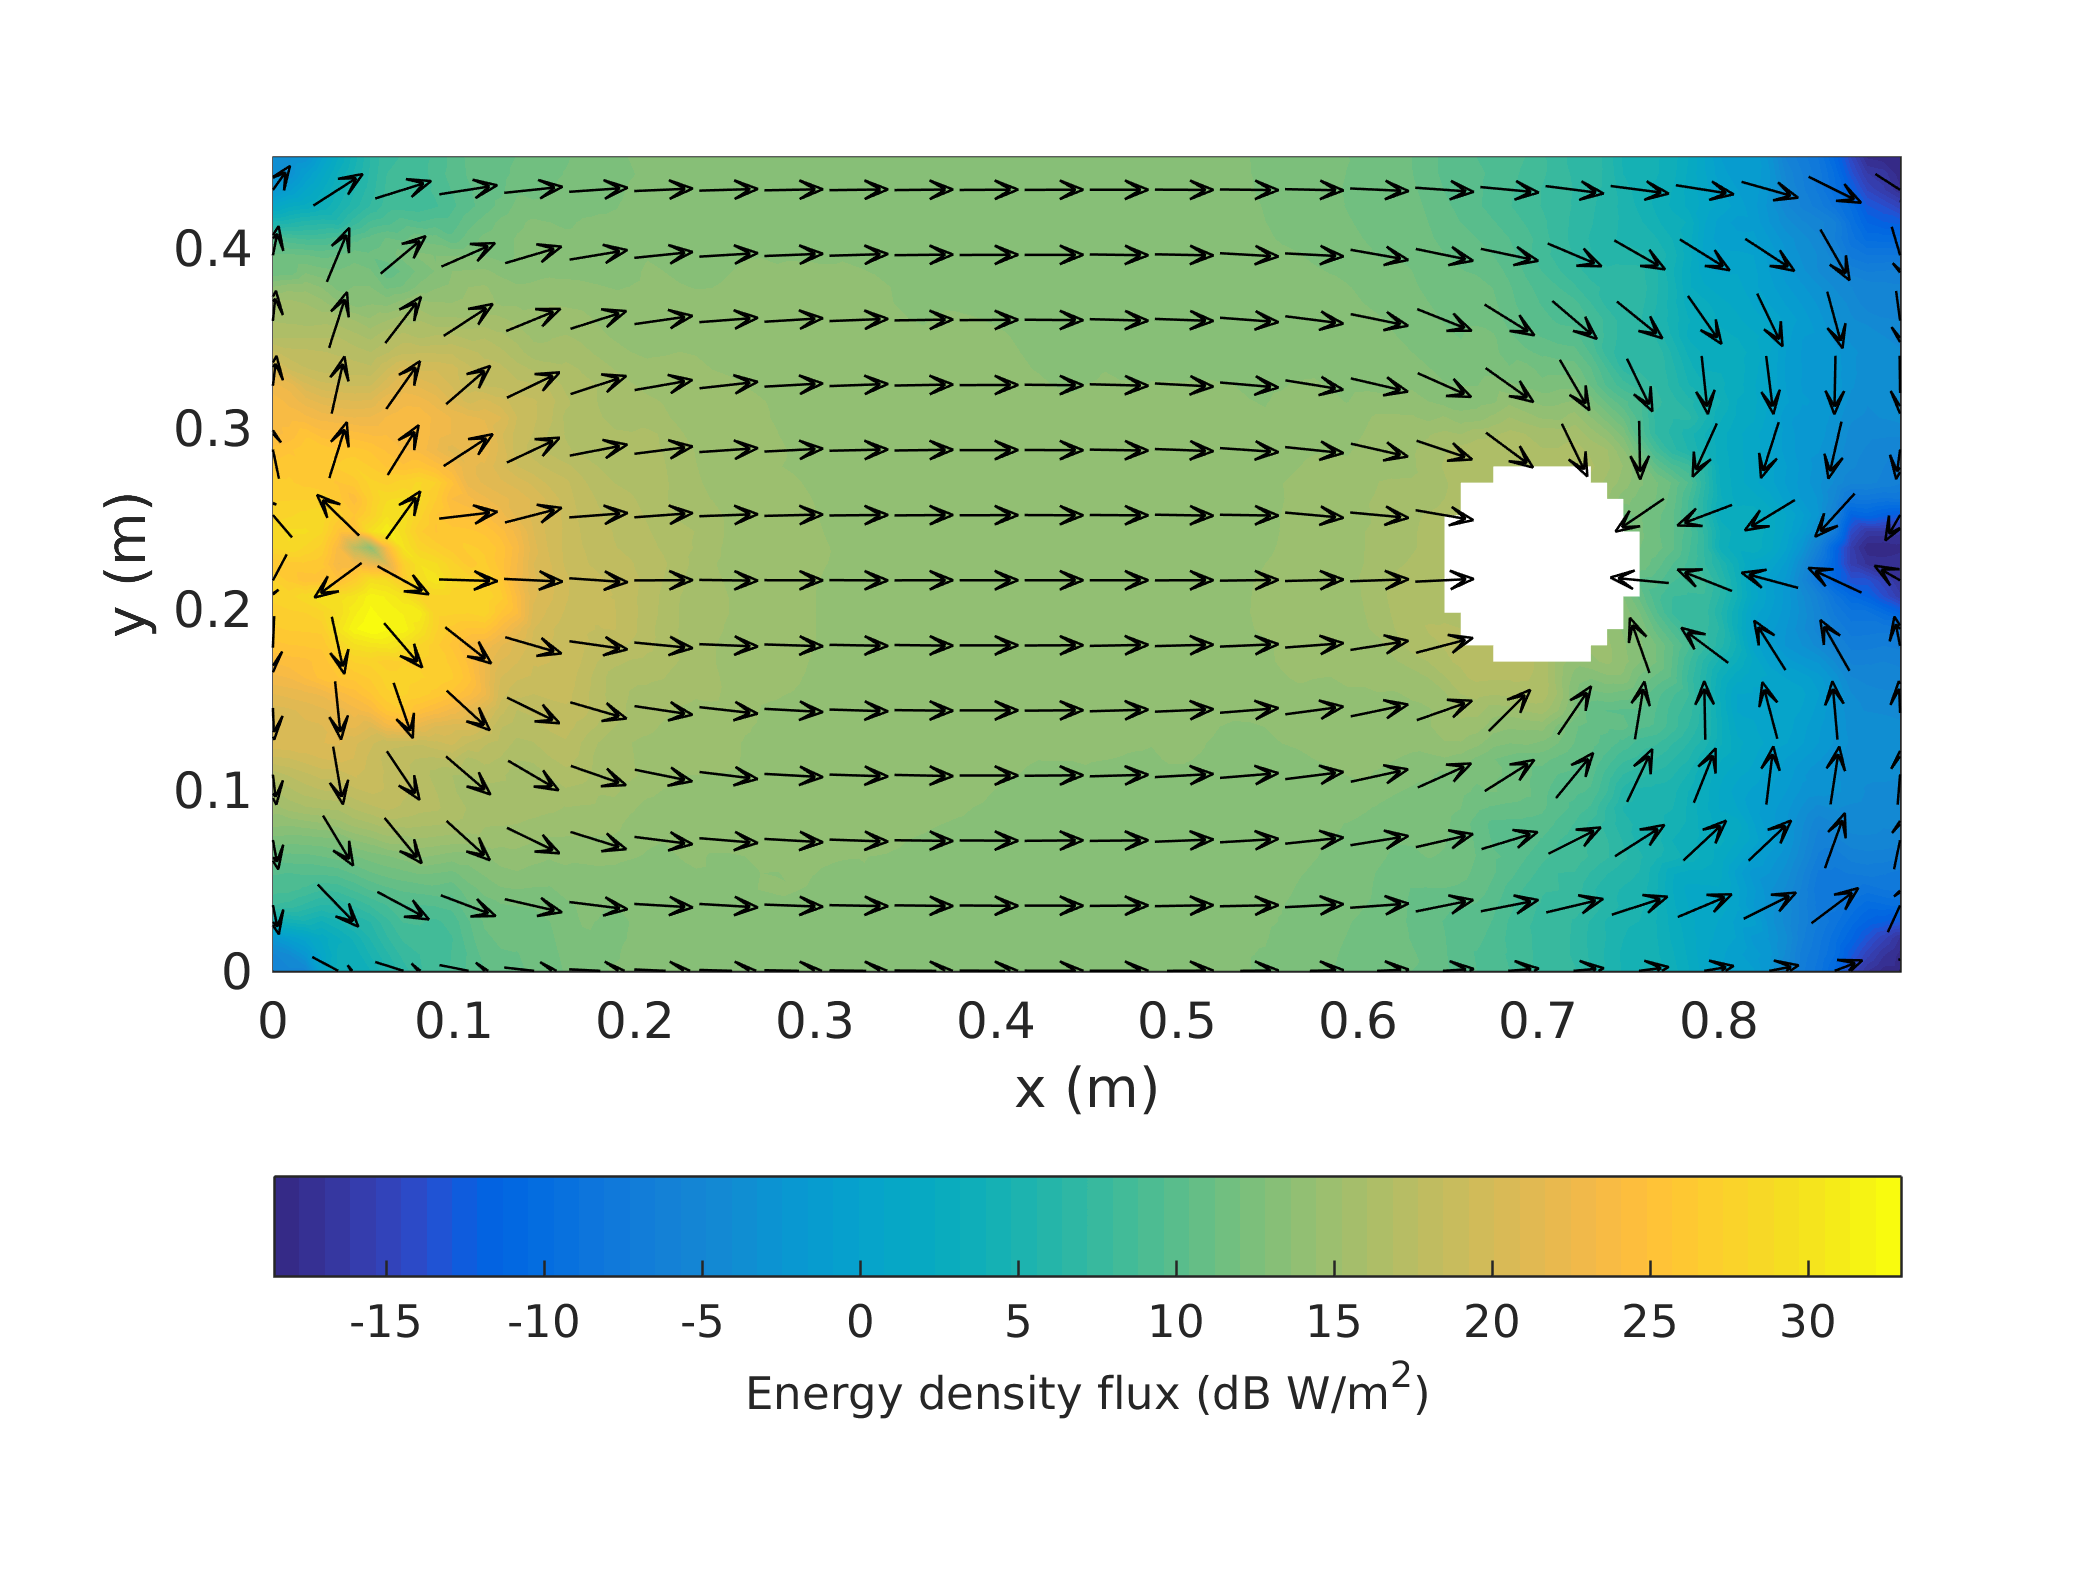
\includegraphics[trim={0 8mm 0 12mm},clip,width=0.52\linewidth]{figures/SDM_3D_SL_EnergyDensityFluxMap}\\
{\footnotesize (d)}\\
\vspace{-2mm}
\caption{\label{fg:unpartcyl_maps} 3D EDM maps in the $z$-normal plane at the half height of the cavity for the 
loaded unpartitioned cavity: (a) Power density; (b) Energy density relative to the homogeneous PWB model;
(c) Anisotropy; (d) Energy density flux.}
\end{center}
\end{figure}

The variation of the power density in the $z$-direction is shown in Figure~\ref{fg:unpartcyl_profs}(a)
at $y=L_y/2$ and various values of $x$. In this case the quadratic anzatz used in the Kantorovich reduction
is seen to be less accurate; however, the 2D model still provides good results. The variation of the power density 
in the $x$ direction for $z=L_z/2$ and a number of $y$ positions is shown in Figure~\ref{fg:unpartempty_profs}(b).
The power density again falls monotonically along the cavity away from the source. At the source end of 
the cavity the EDM predicts higher power density than PWB, while 
at the opposite end the EDM result is a little lower than the PWB result. The average power density in the EDM in 
Table~\ref{tb:unpartempty} is 1.5\,dB higher than the PWB prediction. The probability density function (PDF)
for the average power density in the cavity is shown in Figure~\ref{fg:unpartempty_profs}(c); it is a relatively
uniform distribution.

Figure~\ref{fg:unpartcyl_maps} shows maps of various quantities in the $z=L_z/2$ plane. The power density
shown in Figure~\ref{fg:unpartcyl_maps}(a) exhibits a monotonic decrease along the cavity, with a shadow
region behind the cylinder. The uniformity shown in Figure~\ref{fg:unpartcyl_maps}(b)
is the ratio of the EDM and PWB power densities. The zero isoline is close to the cylinder indicating that in most of 
the cavity the EDM power density is higher than the PWB power density. The anisotropy of the power density is shown in
Figure~\ref{fg:unpartcyl_maps}(c); it is much higher than for the unloaded cavity with a typically value of 0.5\,dB.
Figure~\ref{fg:unpartcyl_maps}(c) shows the flux of the energy density, which clearly shows the flow of reverberant power from 
the source to the cylinder. 

\subsection[Empty partitioned cavity]{Empty partitioned cavity}
\label{sc:res:emptypart}

The derived parameters empty for the partitioned cavity are given in Table~\ref{tb:derivparamdu} and the summary 
statistics for the average power density in the EDM models are presented in Table~\ref{tb:partempty}. 
Results are given for 2D and 3D SDM cases, EEBC and SDM models for the hole, and also for the homogeneous 
PWB model. 

The power density is fairly uniform within each sub-cavity, with a COV of about 0.65\,\% in the source cavity
and a slightly lower value of 0.45\,\% in the coupled cavity. The 2D and 3D models are in very close agreement
and the EEBC and SDM models only differ by about 1\,\%.

\begin{table}[h]
\begin{center}
\begin{tabular}{|c|c|c|c|}
\hline
\textbf{Parameter}     &\textbf{Unit} &\textbf{Source sub-cavity} &\textbf{Coupled sub-cavity}\\ 
\hline
\texttt{wallArea}      &m$^2$         &1.0080                     &1.0080              \\
\texttt{partArea}      &m$^2$         &0.1845                     &0.1845              \\
\texttt{holeArea}      &m$^2$         &0.0180                     &0.0180              \\
\texttt{cavityArea}    &m$^2$         &1.2105                     &1.2105              \\
\texttt{cavityVolume}  &m$^3$         &0.090619                   &0.090619            \\
\texttt{wallMFP}       &m             &0.35960                    &0.35960             \\
\texttt{partMFP}       &m             &1.9646                     &1.9646              \\
\texttt{cavityMFP}     &m             &0.29944                    &0.29944             \\
\texttt{wallD}         &m$^2$/s       &3.5935$\times 10^7$        &3.5935$\times 10^7$ \\
\texttt{partD}         &m$^2$/s       &1.9633$\times 10^8$        &1.9633$\times 10^8$ \\
\texttt{cavityD}       &m$^2$/s       &2.9924$\times 10^7$        &2.9924$\times 10^7$ \\
\texttt{wallACS}       &m$^2$         &0.00068040                 &0.00068040          \\
\texttt{partACS}       &m$^2$         &0.00012454                 &0.00012454          \\
\texttt{cavityACS}     &m$^2$         &0.00080494                 &0.00080494          \\
\hline
\end{tabular}
\end{center}
\caption{\label{tb:derivparamdu} Derived parameters for the unloaded partitioned cavity.}
\end{table}

\begin{table}[h]
\begin{center}
\begin{tabular}{|l|c|c|c|c|c|}
\hline
\textbf{Power density}               &\textbf{PWB} &\multicolumn{4}{|c|}{\textbf{EDM}} \\ \cline{3-6}
{}                                   &{}           &\textbf{2D SDM} &\textbf{2D DDM} &\textbf{3D SDM} &\textbf{3D DDM} \\
\hline
\multicolumn{6}{|l|}{\textbf{Sub-cavity 1}} \\
\hline
Value at centre (dB\,W\,m$^{-2})$    &28.27        &28.04           &28.37           &28.03           &28.36 \\
Mean (dB\,W\,m$^{-2})$               &28.27        &28.04           &28.36           &28.03           &28.36 \\
Minimum (dB\,W\,m$^{-2})$            &28.27        &27.89           &28.24           &26.93           &27.35 \\
Maximum (dB\,W\,m$^{-2})$            &28.27        &28.11           &28.43           &28.14           &28.47 \\
Standard deviation (dB\,W\,m$^{-2})$ &0            &6.47            &6.28            &5.95            &5.76  \\
Coefficient of variation (\%)        &0            &0.70            &0.62            &0.62            &0.55  \\
\hline
\multicolumn{6}{|l|}{\textbf{Sub-cavity 2}} \\
\hline
Value at centre (dB\,W\,m$^{-2})$    &27.55        &27.78           &27.42           &27.78           &27.42 \\
Mean (dB\,W\,m$^{-2})$               &27.55        &27.79           &27.43           &27.79           &27.43 \\
Minimum (dB\,W\,m$^{-2})$            &27.55        &27.76           &27.41           &27.77           &27.41 \\
Maximum (dB\,W\,m$^{-2})$            &27.55        &27.89           &27.55           &27.90           &27.55 \\
Standard deviation (dB\,W\,m$^{-2})$ &0            &4.17            &3.85            &4.16            &3.85  \\
Coefficient of variation (\%)        &0            &0.44            &0.44            &0.43            &0.44  \\
\hline
\end{tabular}
\end{center}
\caption{\label{tb:partempty} Statistics of the reverberant power density in the unloaded partitioned cavity.}
\end{table}

The variation of the power density in the $z$-direction for the SDM and EEBC models are shown in 
Figure~\ref{fg:partemptysdm_profs}(a) and Figure~\ref{fg:partemptyddm_profs}(a) at $y=L_y/2$ and various 
values of $x$. In this case the quadratic anzatz used in the Kantorovich reduction
is seen to be quite accurate and the 2D model provides very good results. The variation of the power density 
in the $x$ direction for $z=L_z/2$ and a number of $y$ positions is shown in Figure~\ref{fg:partemptysdm_profs}(b)
and Figure~\ref{fg:partemptyddm_profs}(b) for the SDM and EEBC. The power density is relatively uniform in each
sub-cavity, falling slightly towards the hole in the source sub-cavity and away from the hole in the coupled 
sub-cavity. In both cases there is a rapid variation in the average power at the hole; however, there is a 
significant difference in the level between the sub-cavities predicted by the SDM and EEBC methods 
of treating the aperture BC. The SDM predicts a much small level difference than the EEBC. The level difference
predicted by the EEBC model is quite close to the PWB model prediction. Forcing continuity of both the energy
density and its flux appears to constrain the level difference between the two cavities, while only enforcing
continuity of the energy density flux allows a greater divergence. The probability density function (PDF)
for the average power density in the sub-cavities are shown in Figure~\ref{fg:partemptysdm_profs}(c) and
Figure~\ref{fg:partemptyddm_profs}(c).

Figure~\ref{fg:partemptysdm_maps} and Figure~\ref{fg:partemptyddm_maps} shows maps of various quantities in 
the $z=L_z/2$ plane for the SDM and EEBC models respectively. The power densities are shown in 
Figure~\ref{fg:partemptysdm_maps}(a) and Figure~\ref{fg:partemptyddm_maps}(a) as hybrid heat and contour maps; 
the power density is seen to fall off along the source sub-cavity towards the aperture and then in the coupled
sub-cavity increase away from the hole. The uniformities in the SDM and EEBC models are shown in 
Figure~\ref{fg:partemptysdm_maps}(b) and Figure~\ref{fg:partemptyddm_maps}(b) as the ratio of the EDM and 
PWB power densities. In both cases the EDM predicts lower values than the PWB model in the source cavity and
higher values in the coupled cavity. The anisotropies are shown in Figure~\ref{fg:partemptysdm_maps}(c) and
Figure~\ref{fg:partemptyddm_maps}(c) and are fairly similar for the two aperture models, as are the energy
density fluxes shown in Figure~\ref{fg:partemptysdm_maps}(c) and Figure~\ref{fg:partemptyddm_maps}(c).

\begin{figure}[hp]
\begin{center}
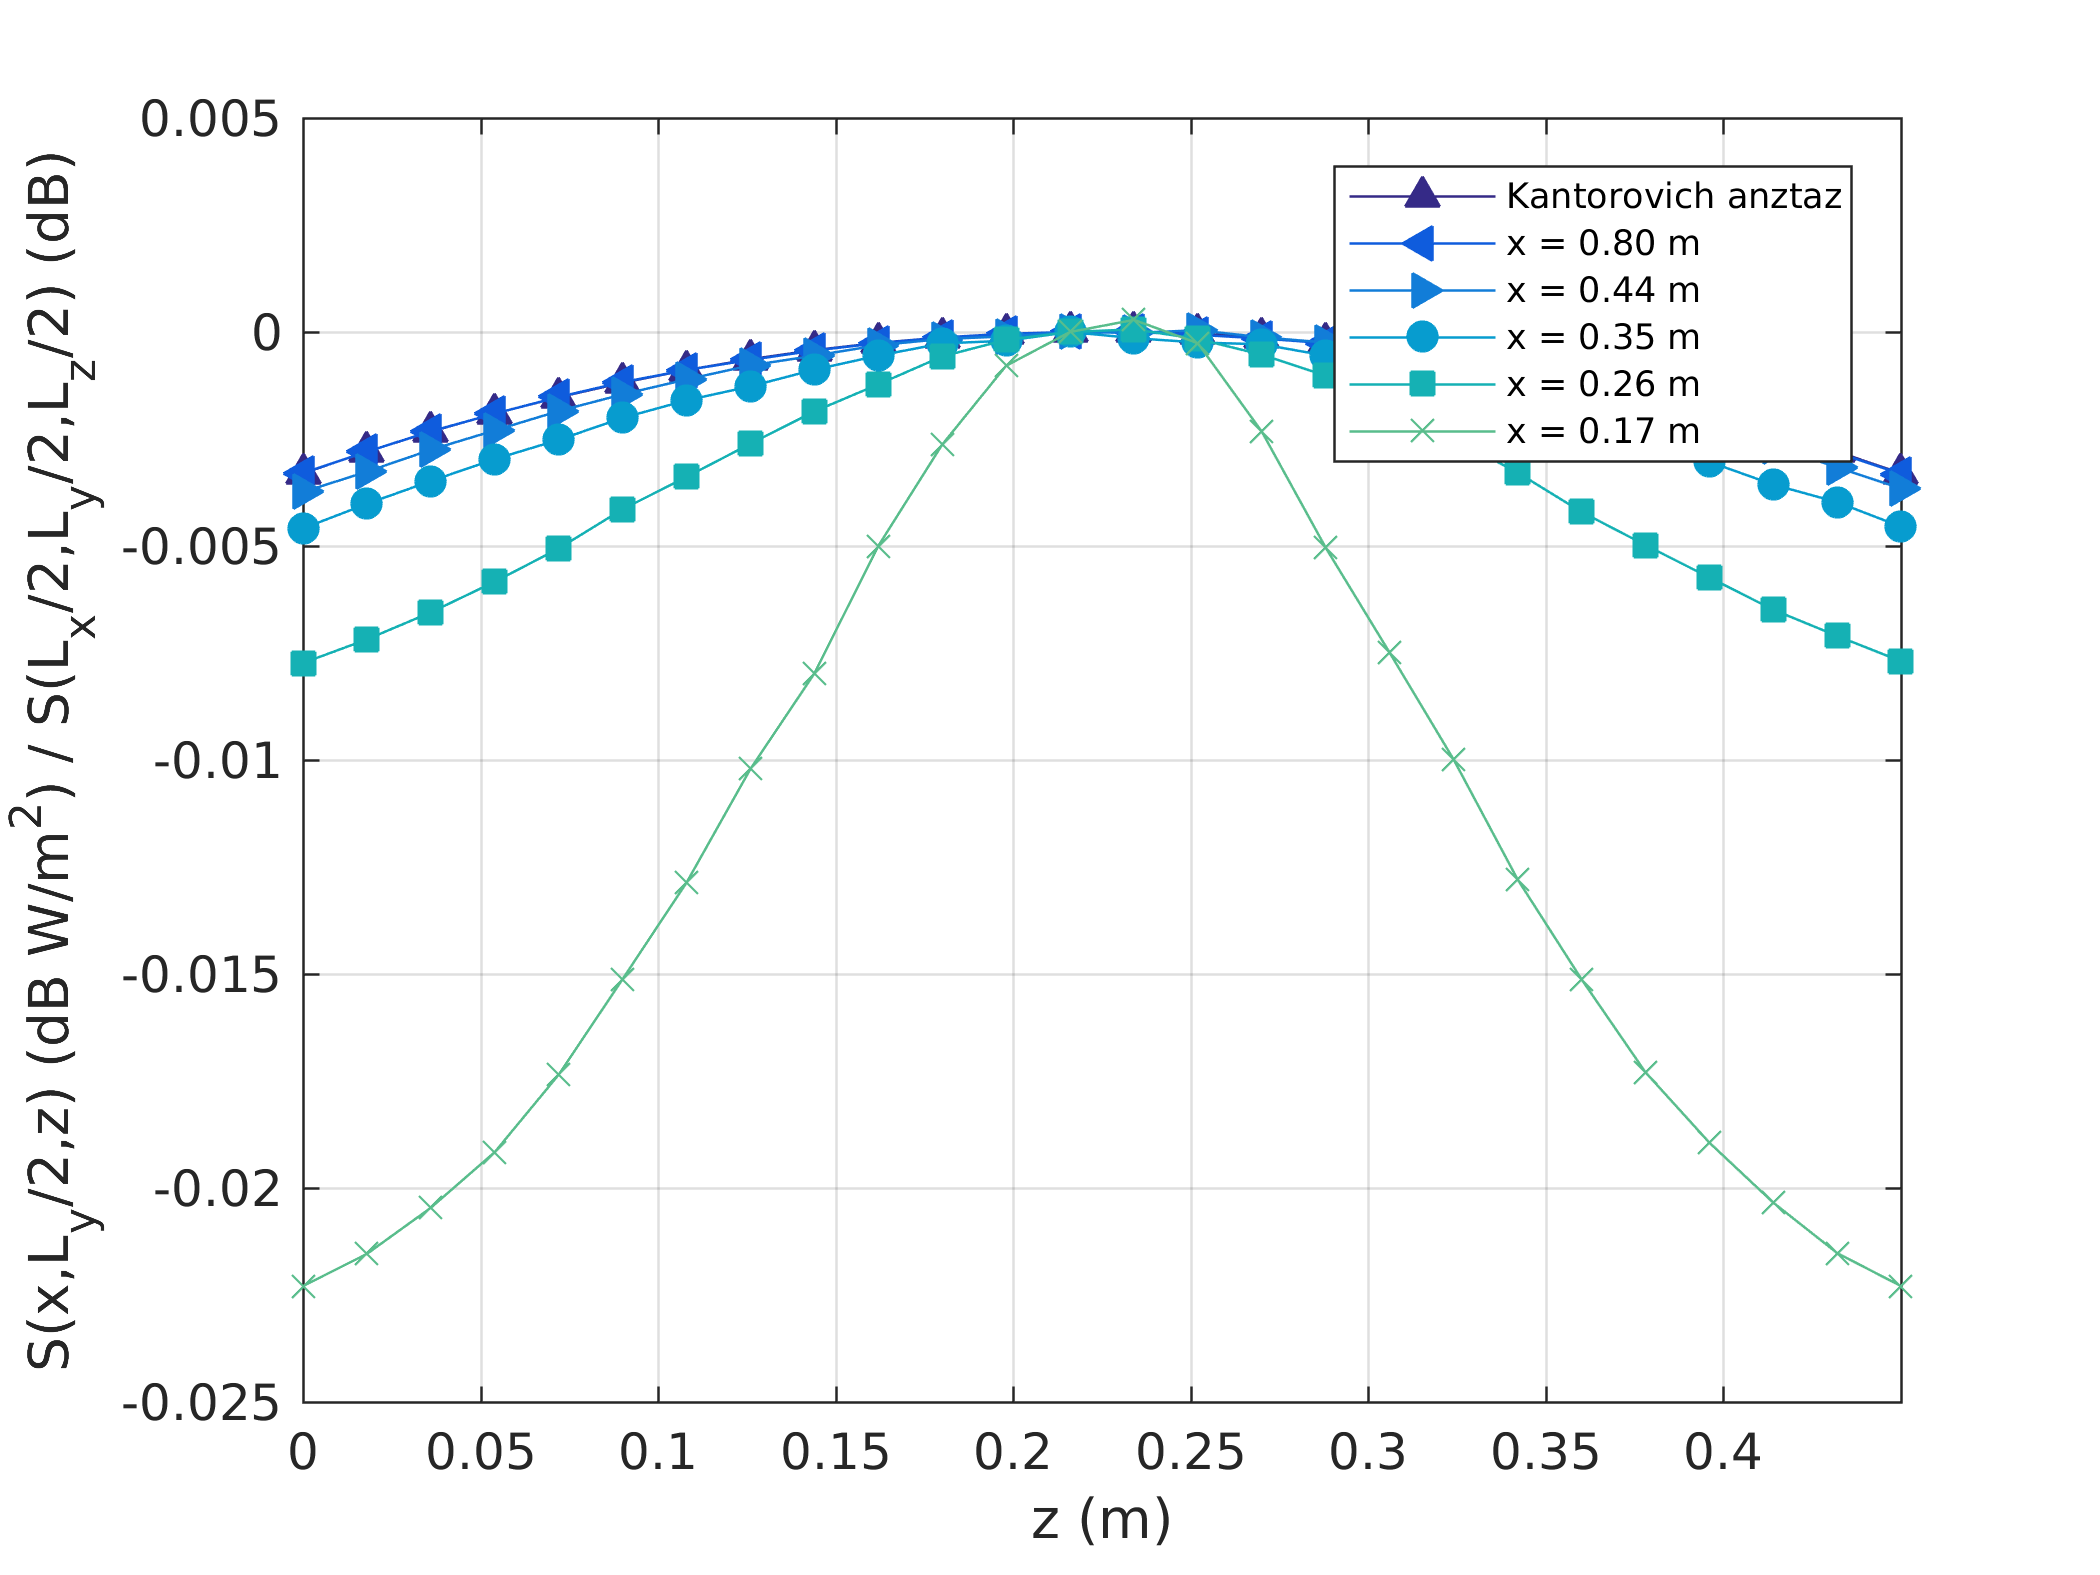
\includegraphics[width=0.6\linewidth]{figures/SDM_3D_DU_PowerDensityProfileZ}\\
{\footnotesize (a)}\\
\vspace{2mm}
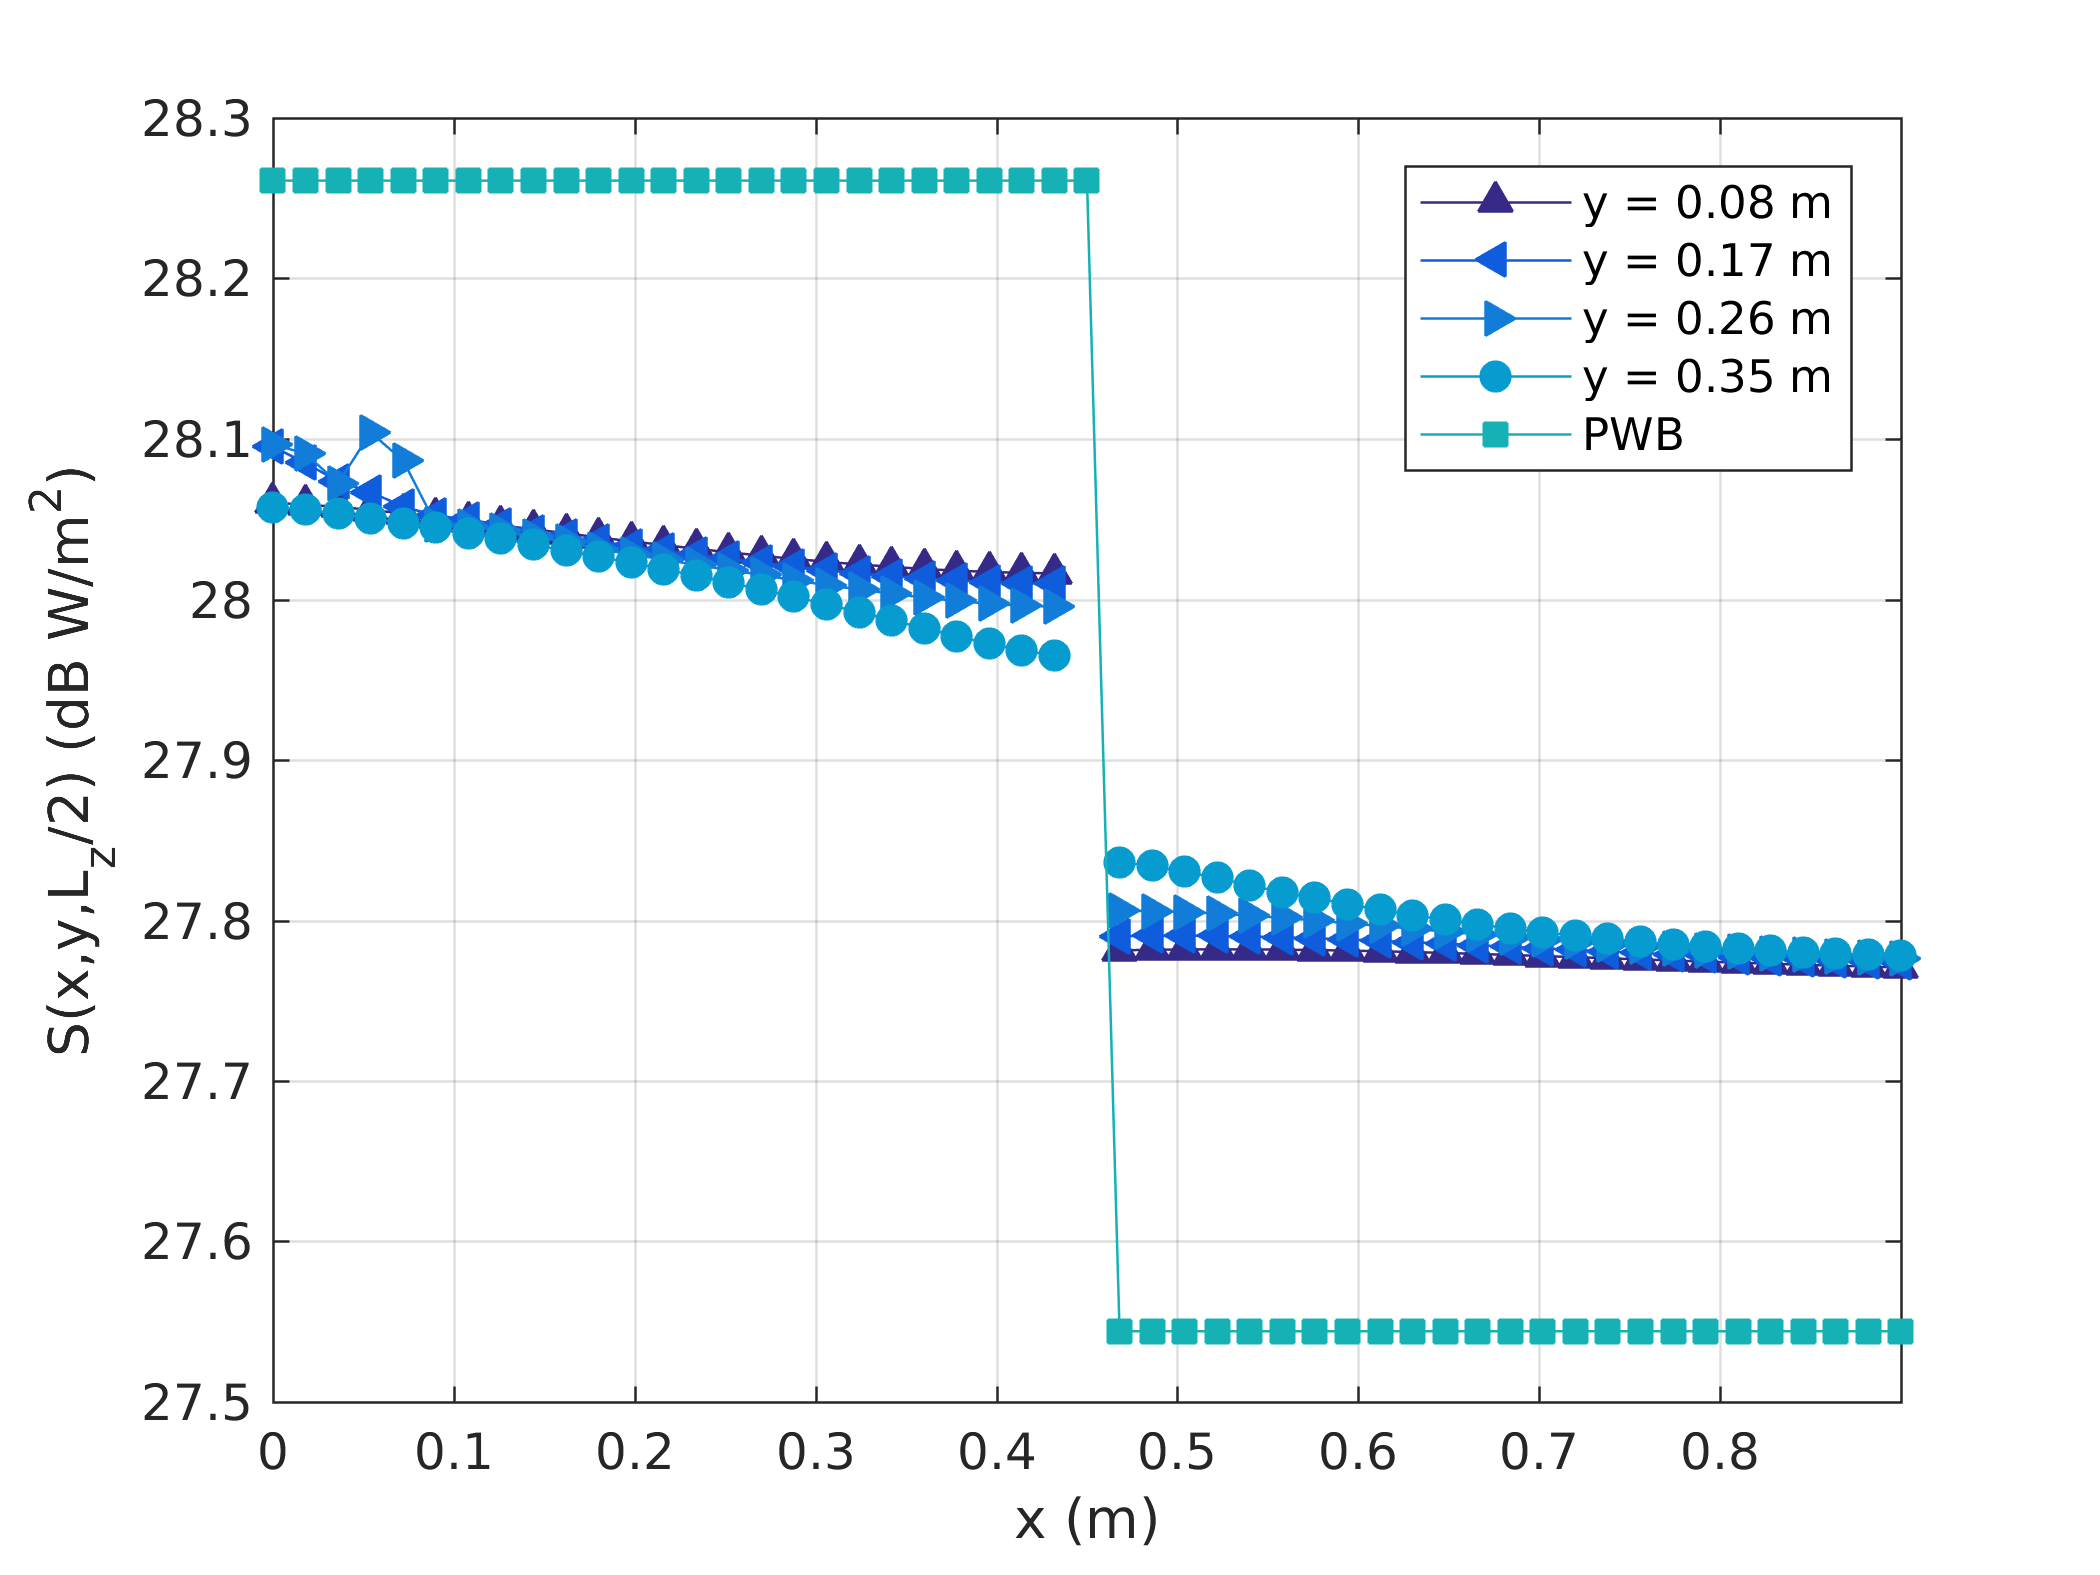
\includegraphics[width=0.6\linewidth]{figures/SDM_3D_DU_PowerDensityProfileX}\\
{\footnotesize (b)}\\
\vspace{2mm}
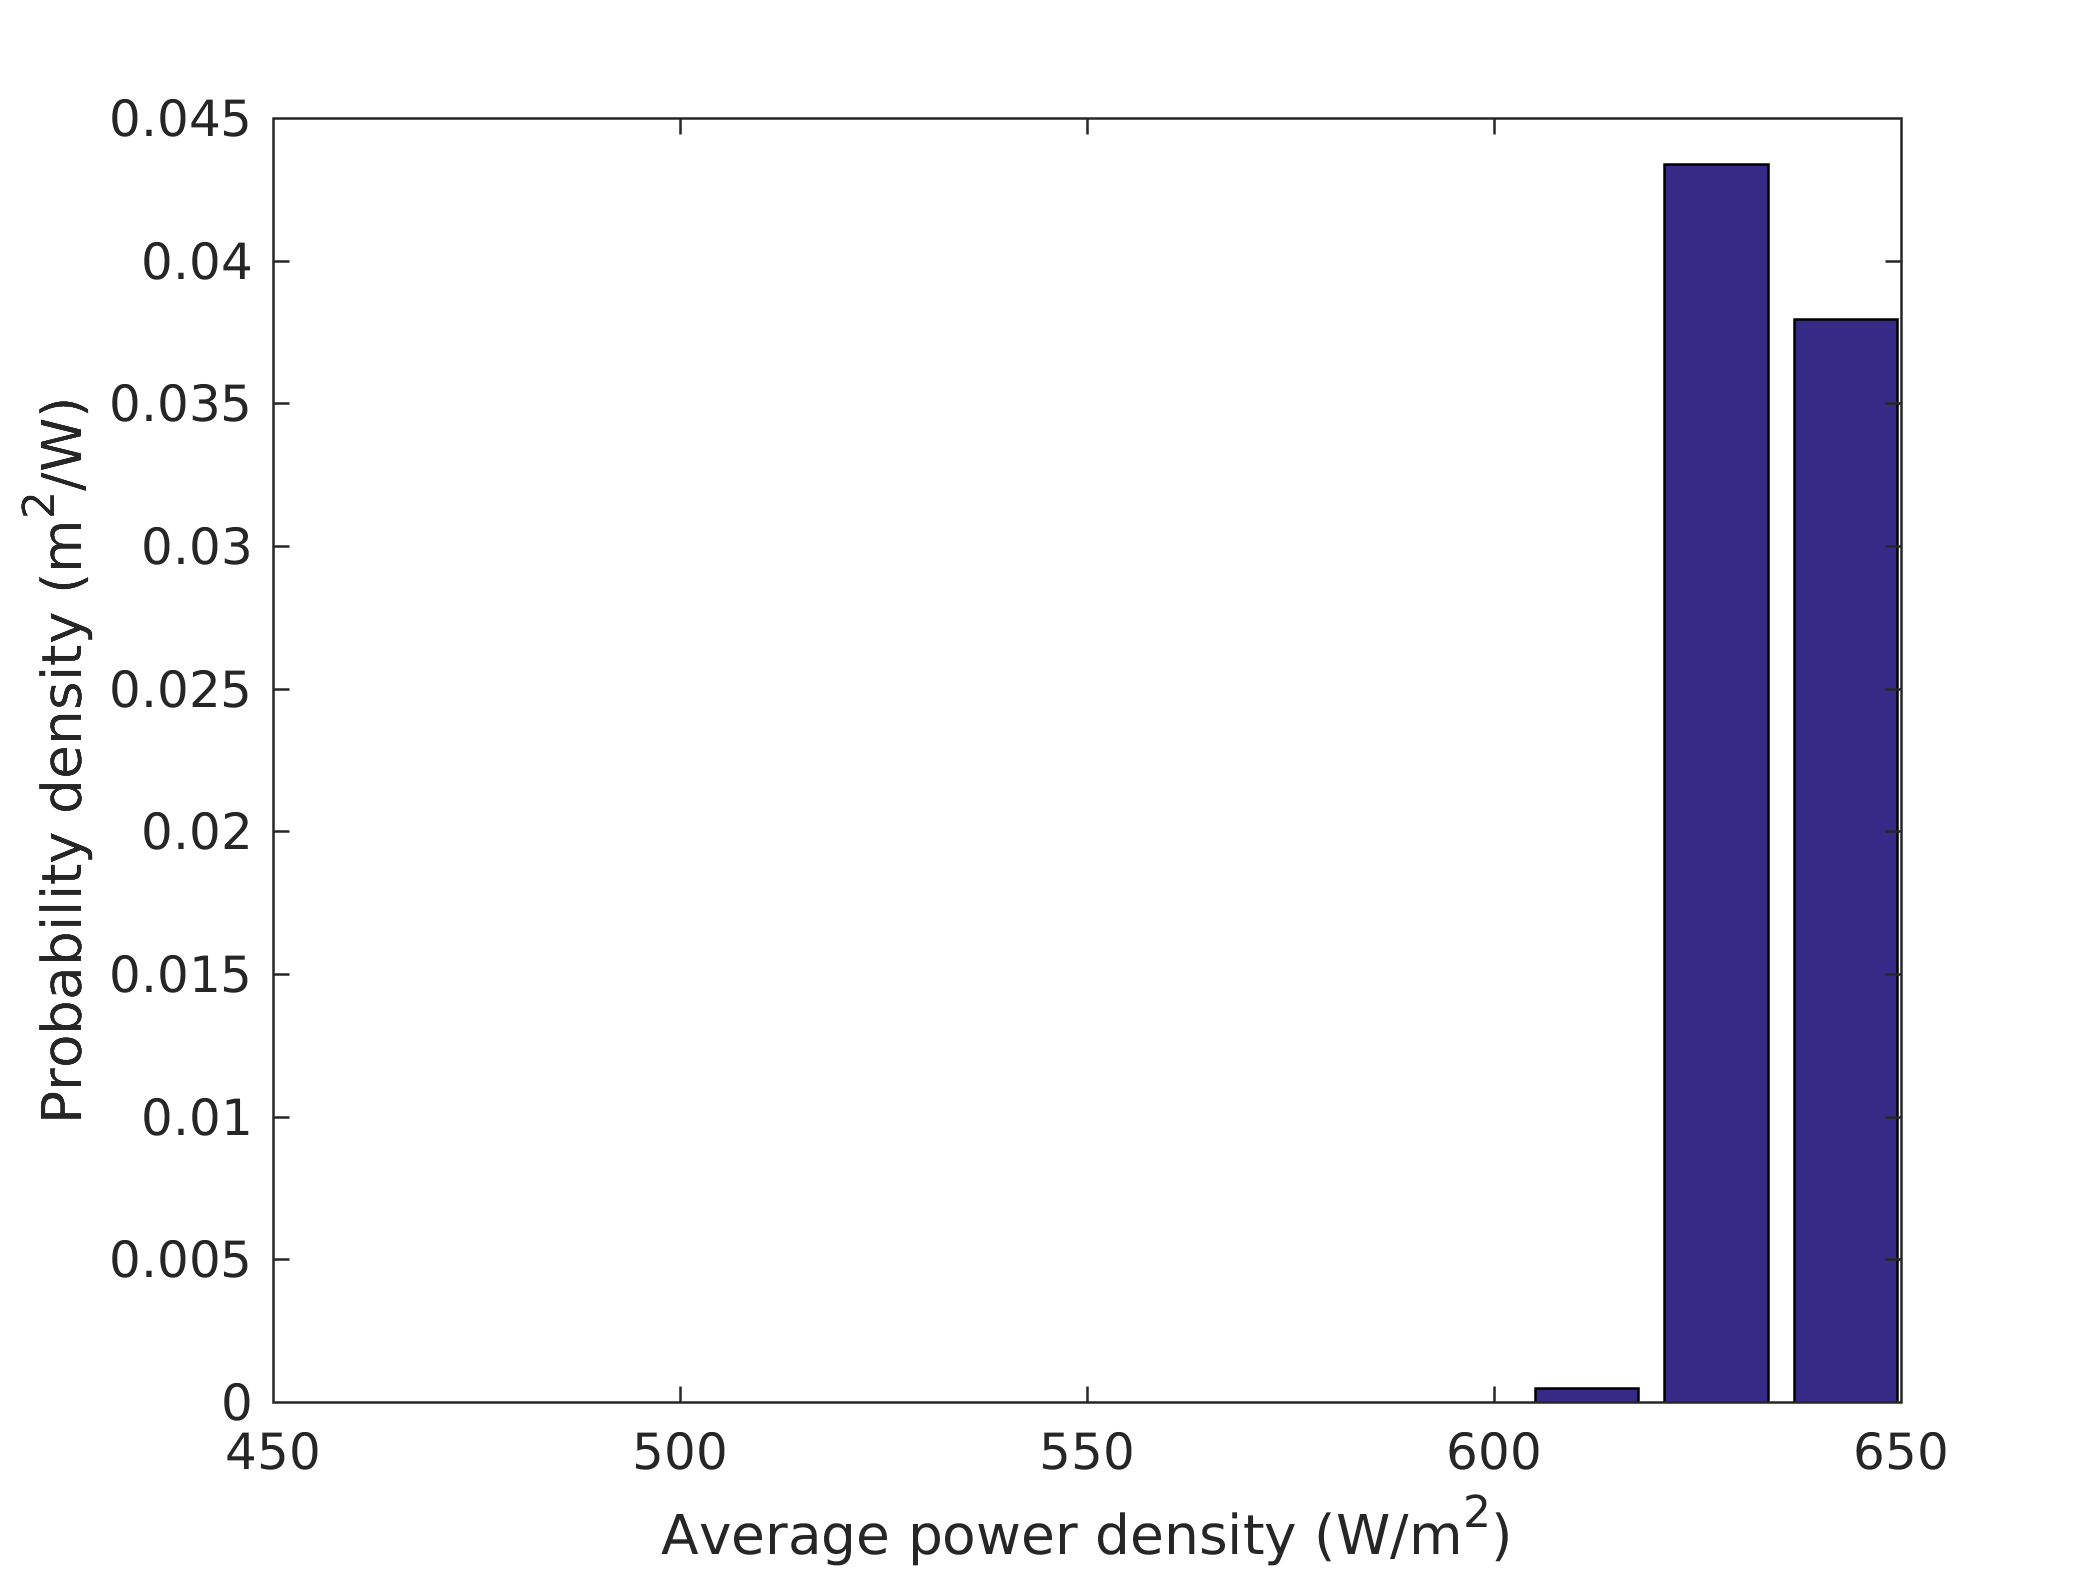
\includegraphics[width=0.45\linewidth]{figures/SDM_3D_DU_PowerDensityPDF1}
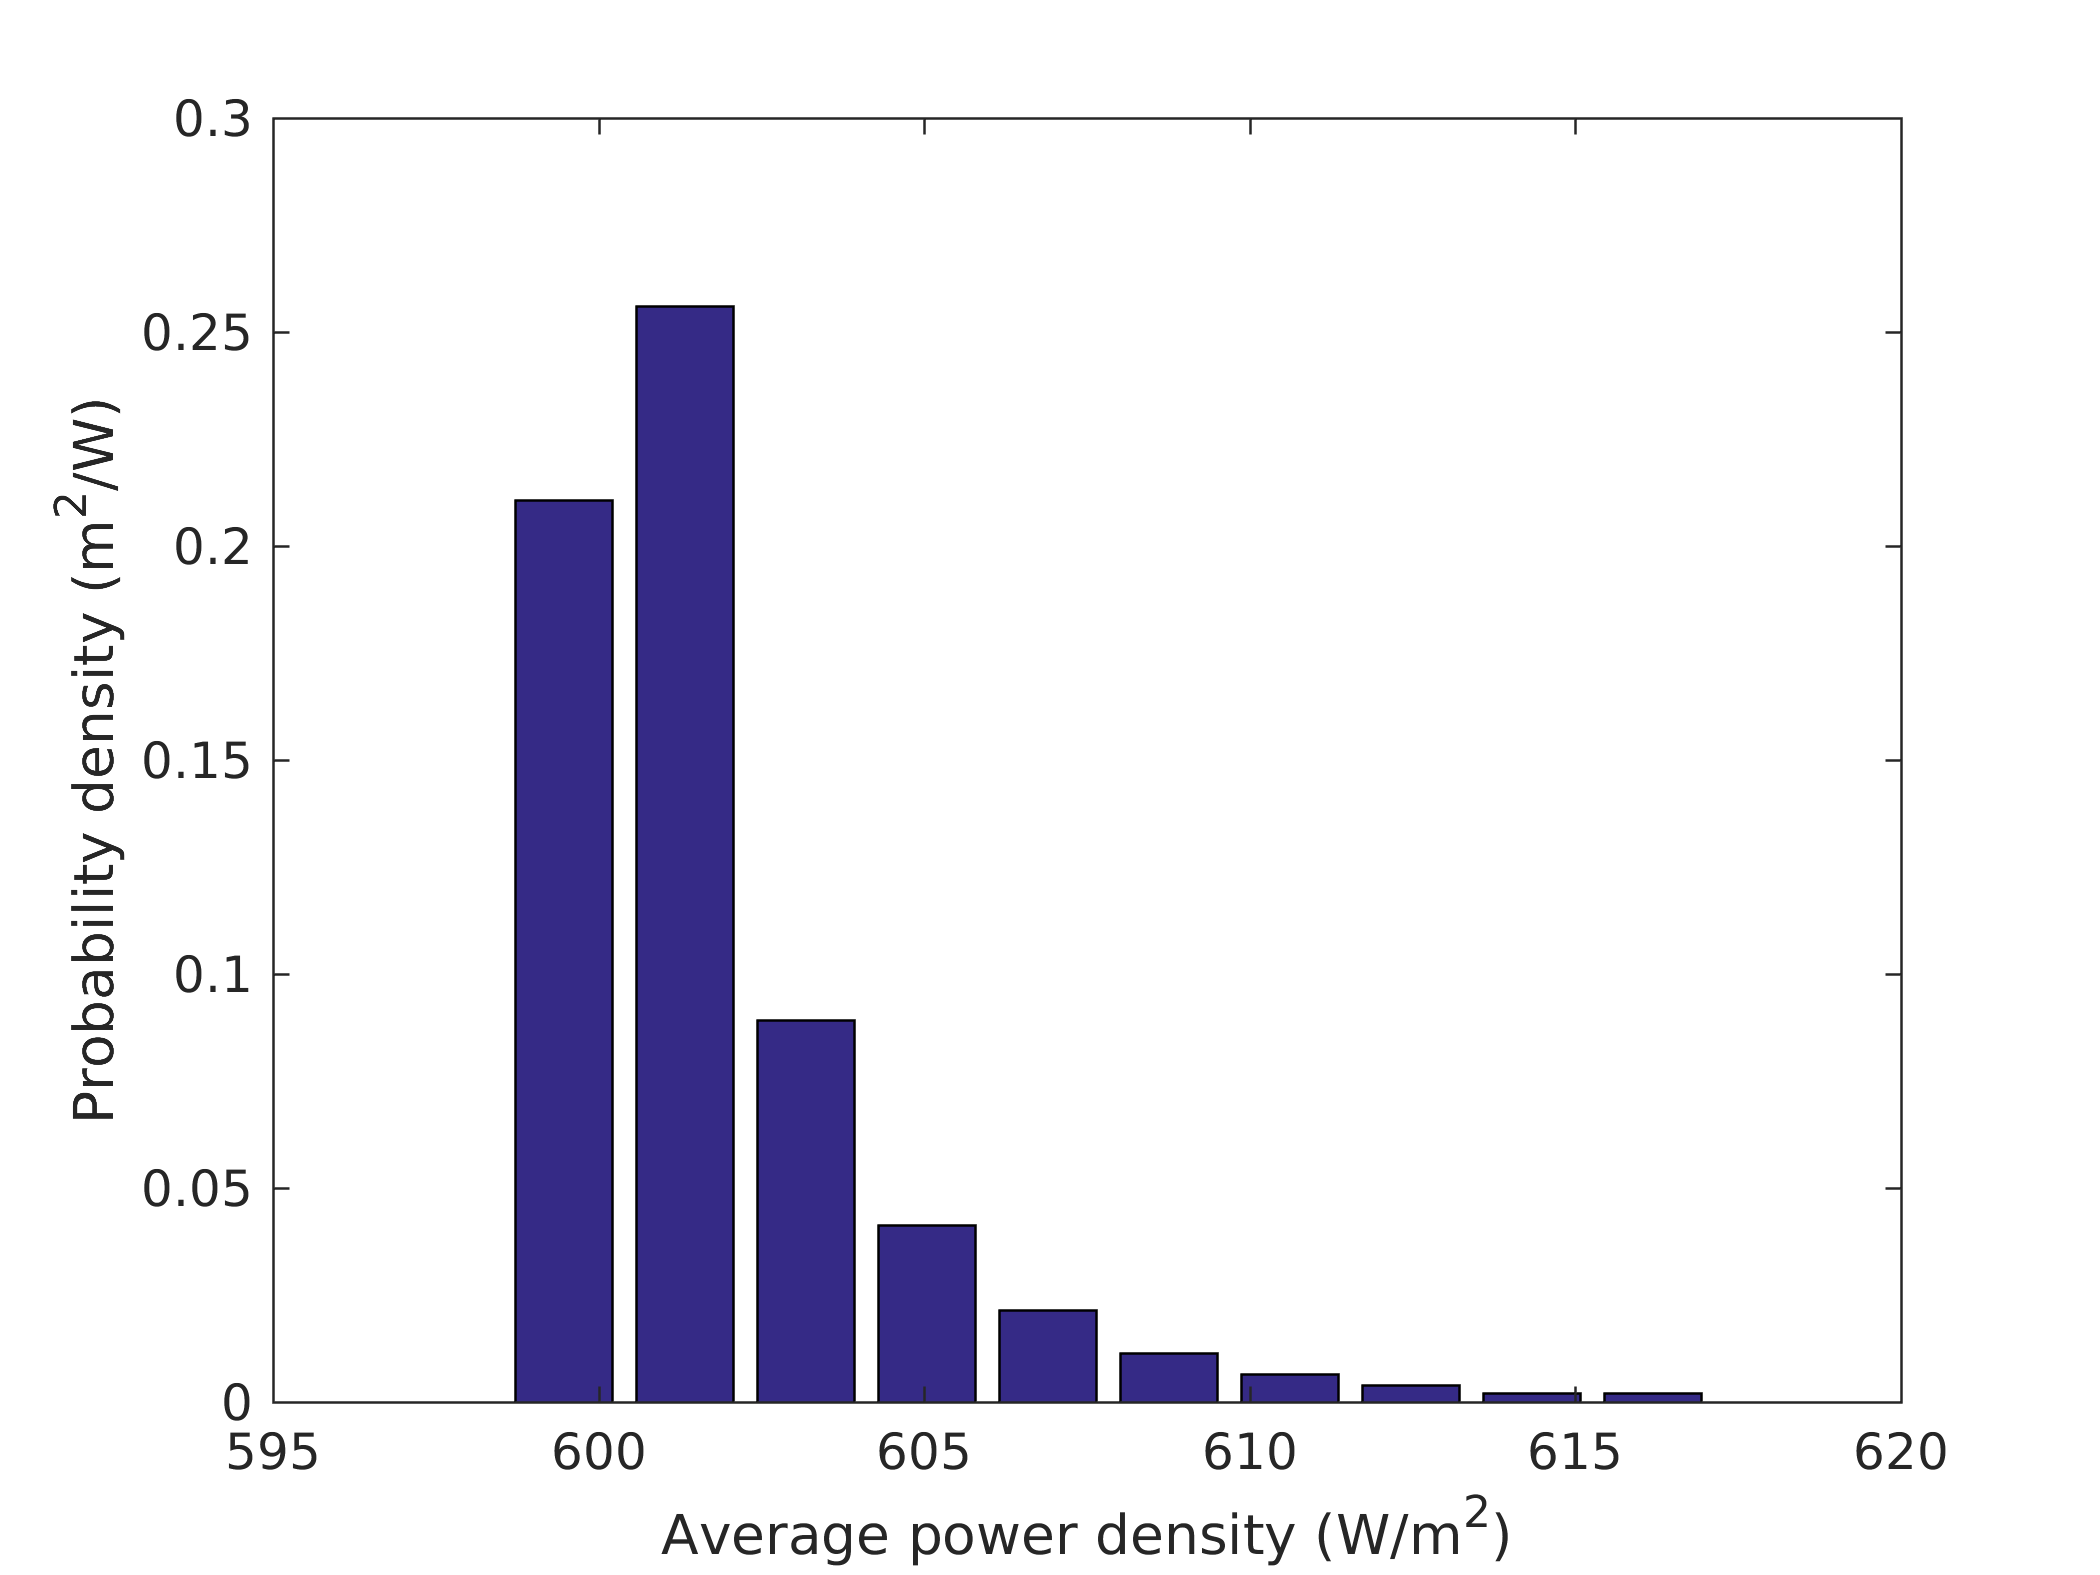
\includegraphics[width=0.45\linewidth]{figures/SDM_3D_DU_PowerDensityPDF2}
\\
{\footnotesize (c)}\\
\vspace{-2mm}
\caption{\label{fg:partemptysdm_profs} Single domain EDM of the unloaded partitioned cavity: (a) Normalised vertical profile of the power density; 
(b) Power density profile in the $x$-direction along the cavity centre; (c) PDF of the power density in the source cavity (left) and coupled cavity (right).}
\end{center}
\end{figure}

\begin{figure}[hp]
\begin{center}
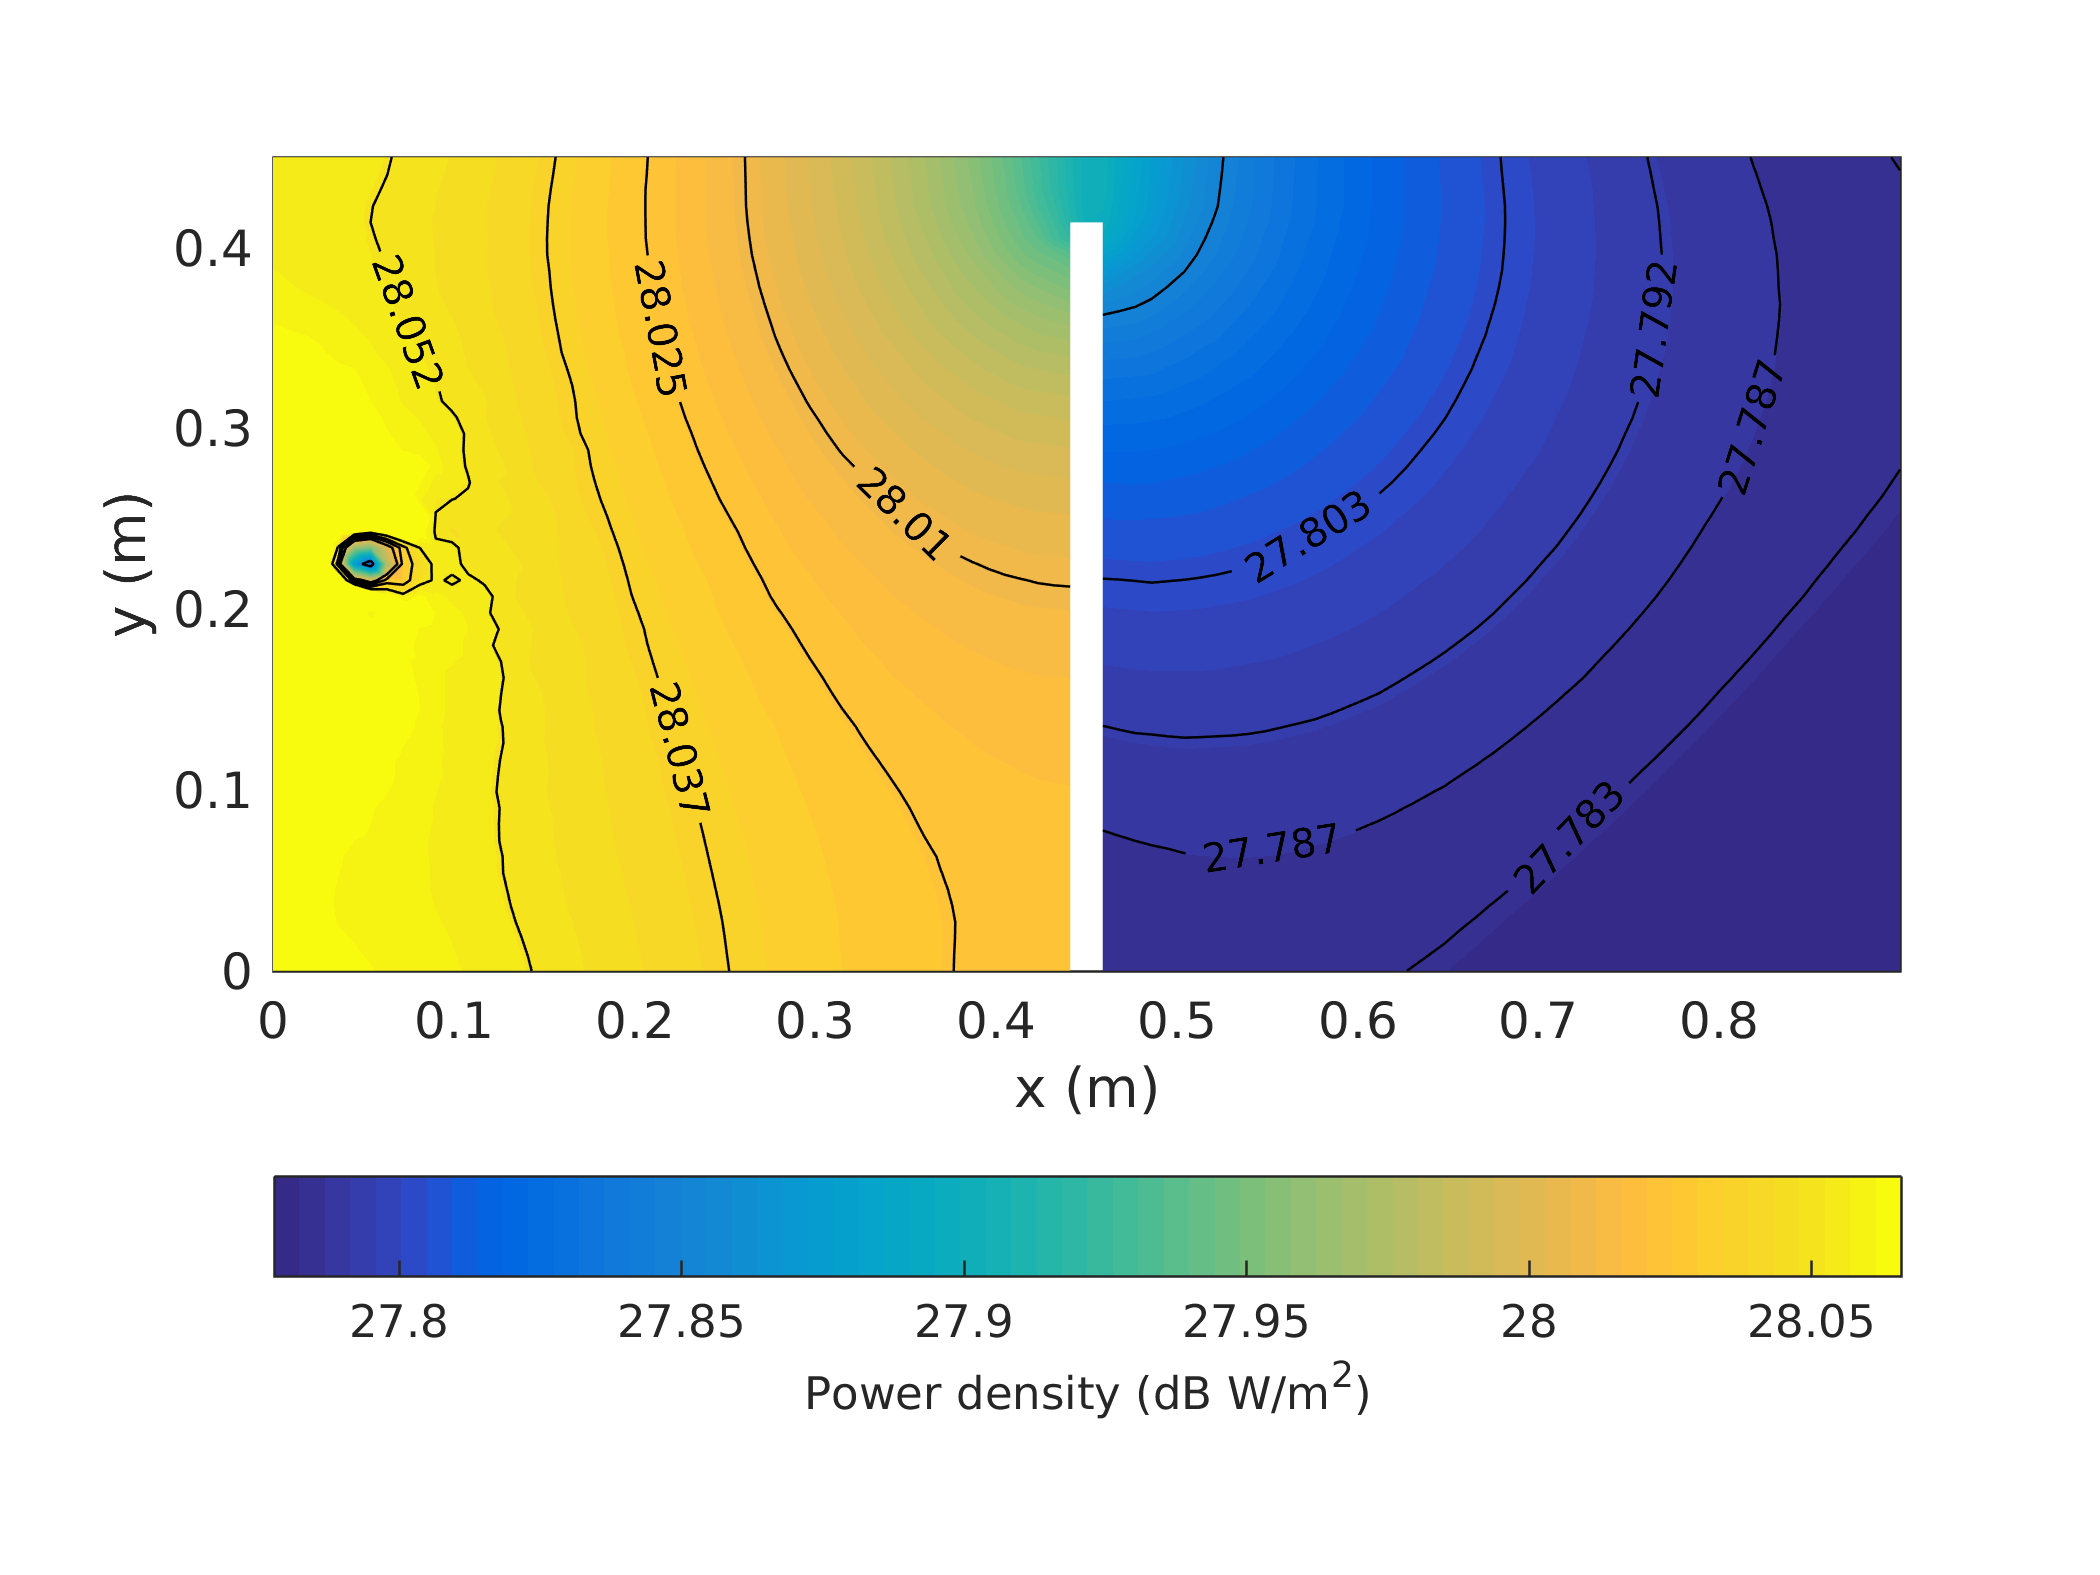
\includegraphics[trim={0 11mm 0 12mm},clip,width=0.52\linewidth]{figures/SDM_3D_DU_PowerDensityMap}\\
{\footnotesize (a)}\\
\vspace{2mm}
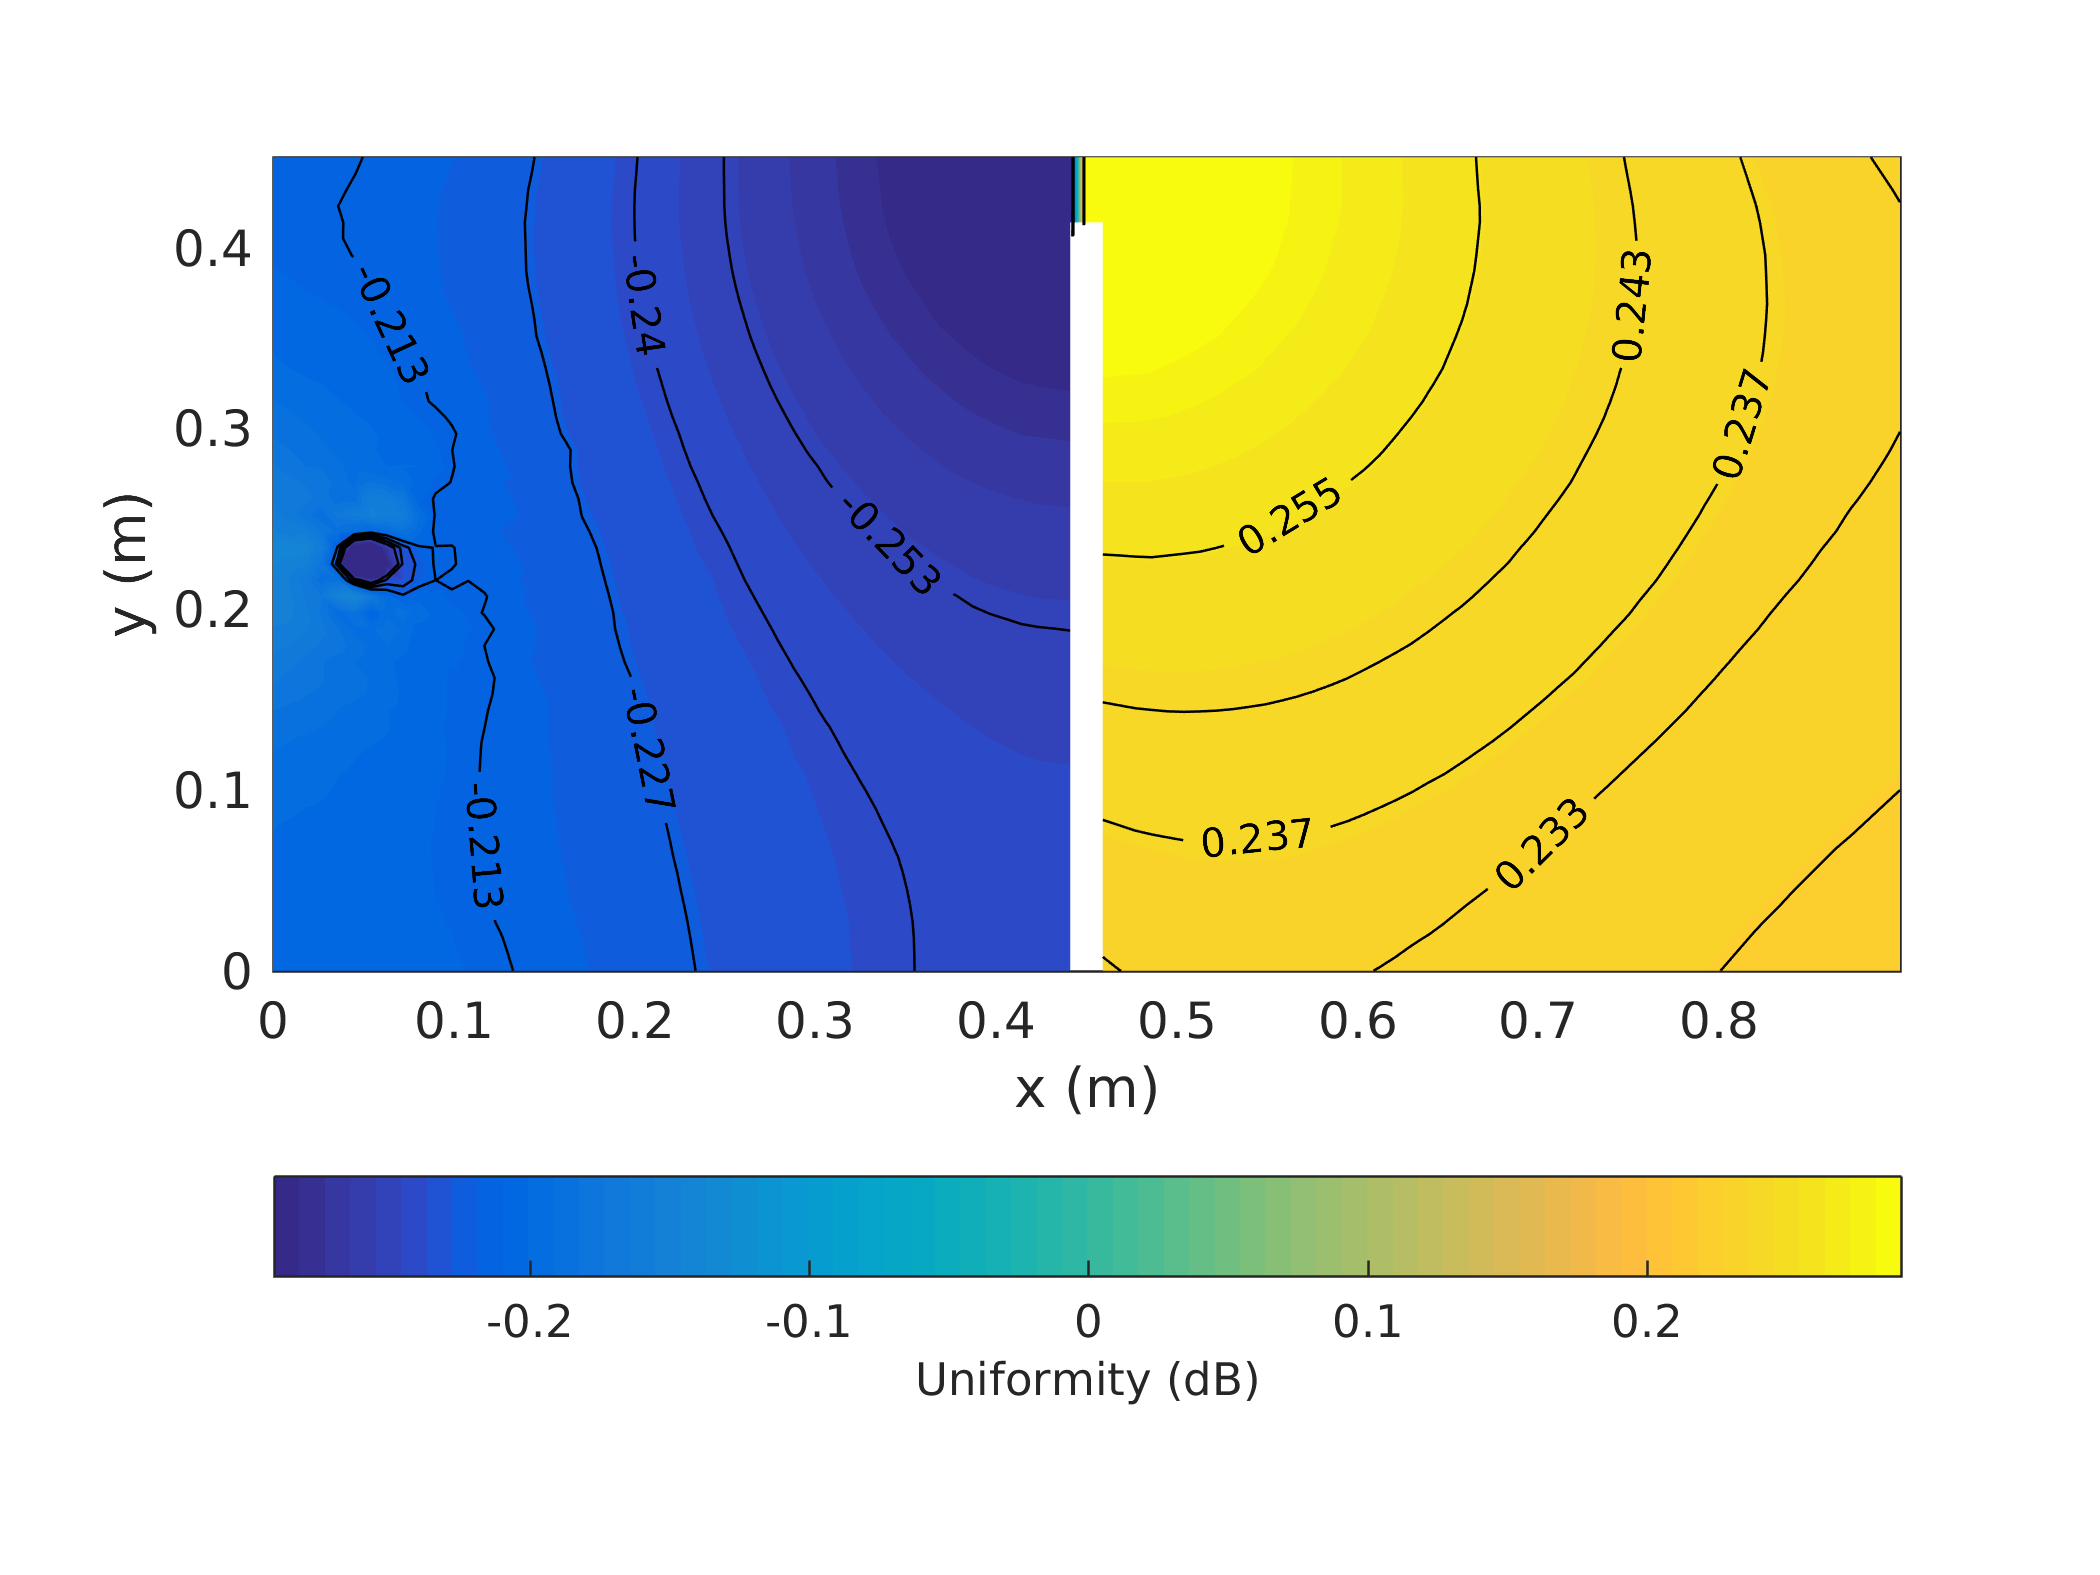
\includegraphics[trim={0 11mm 0 12mm},clip,width=0.52\linewidth]{figures/SDM_3D_DU_EnergyDensityUniformityMap}\\
{\footnotesize (b)}\\
\vspace{2mm}
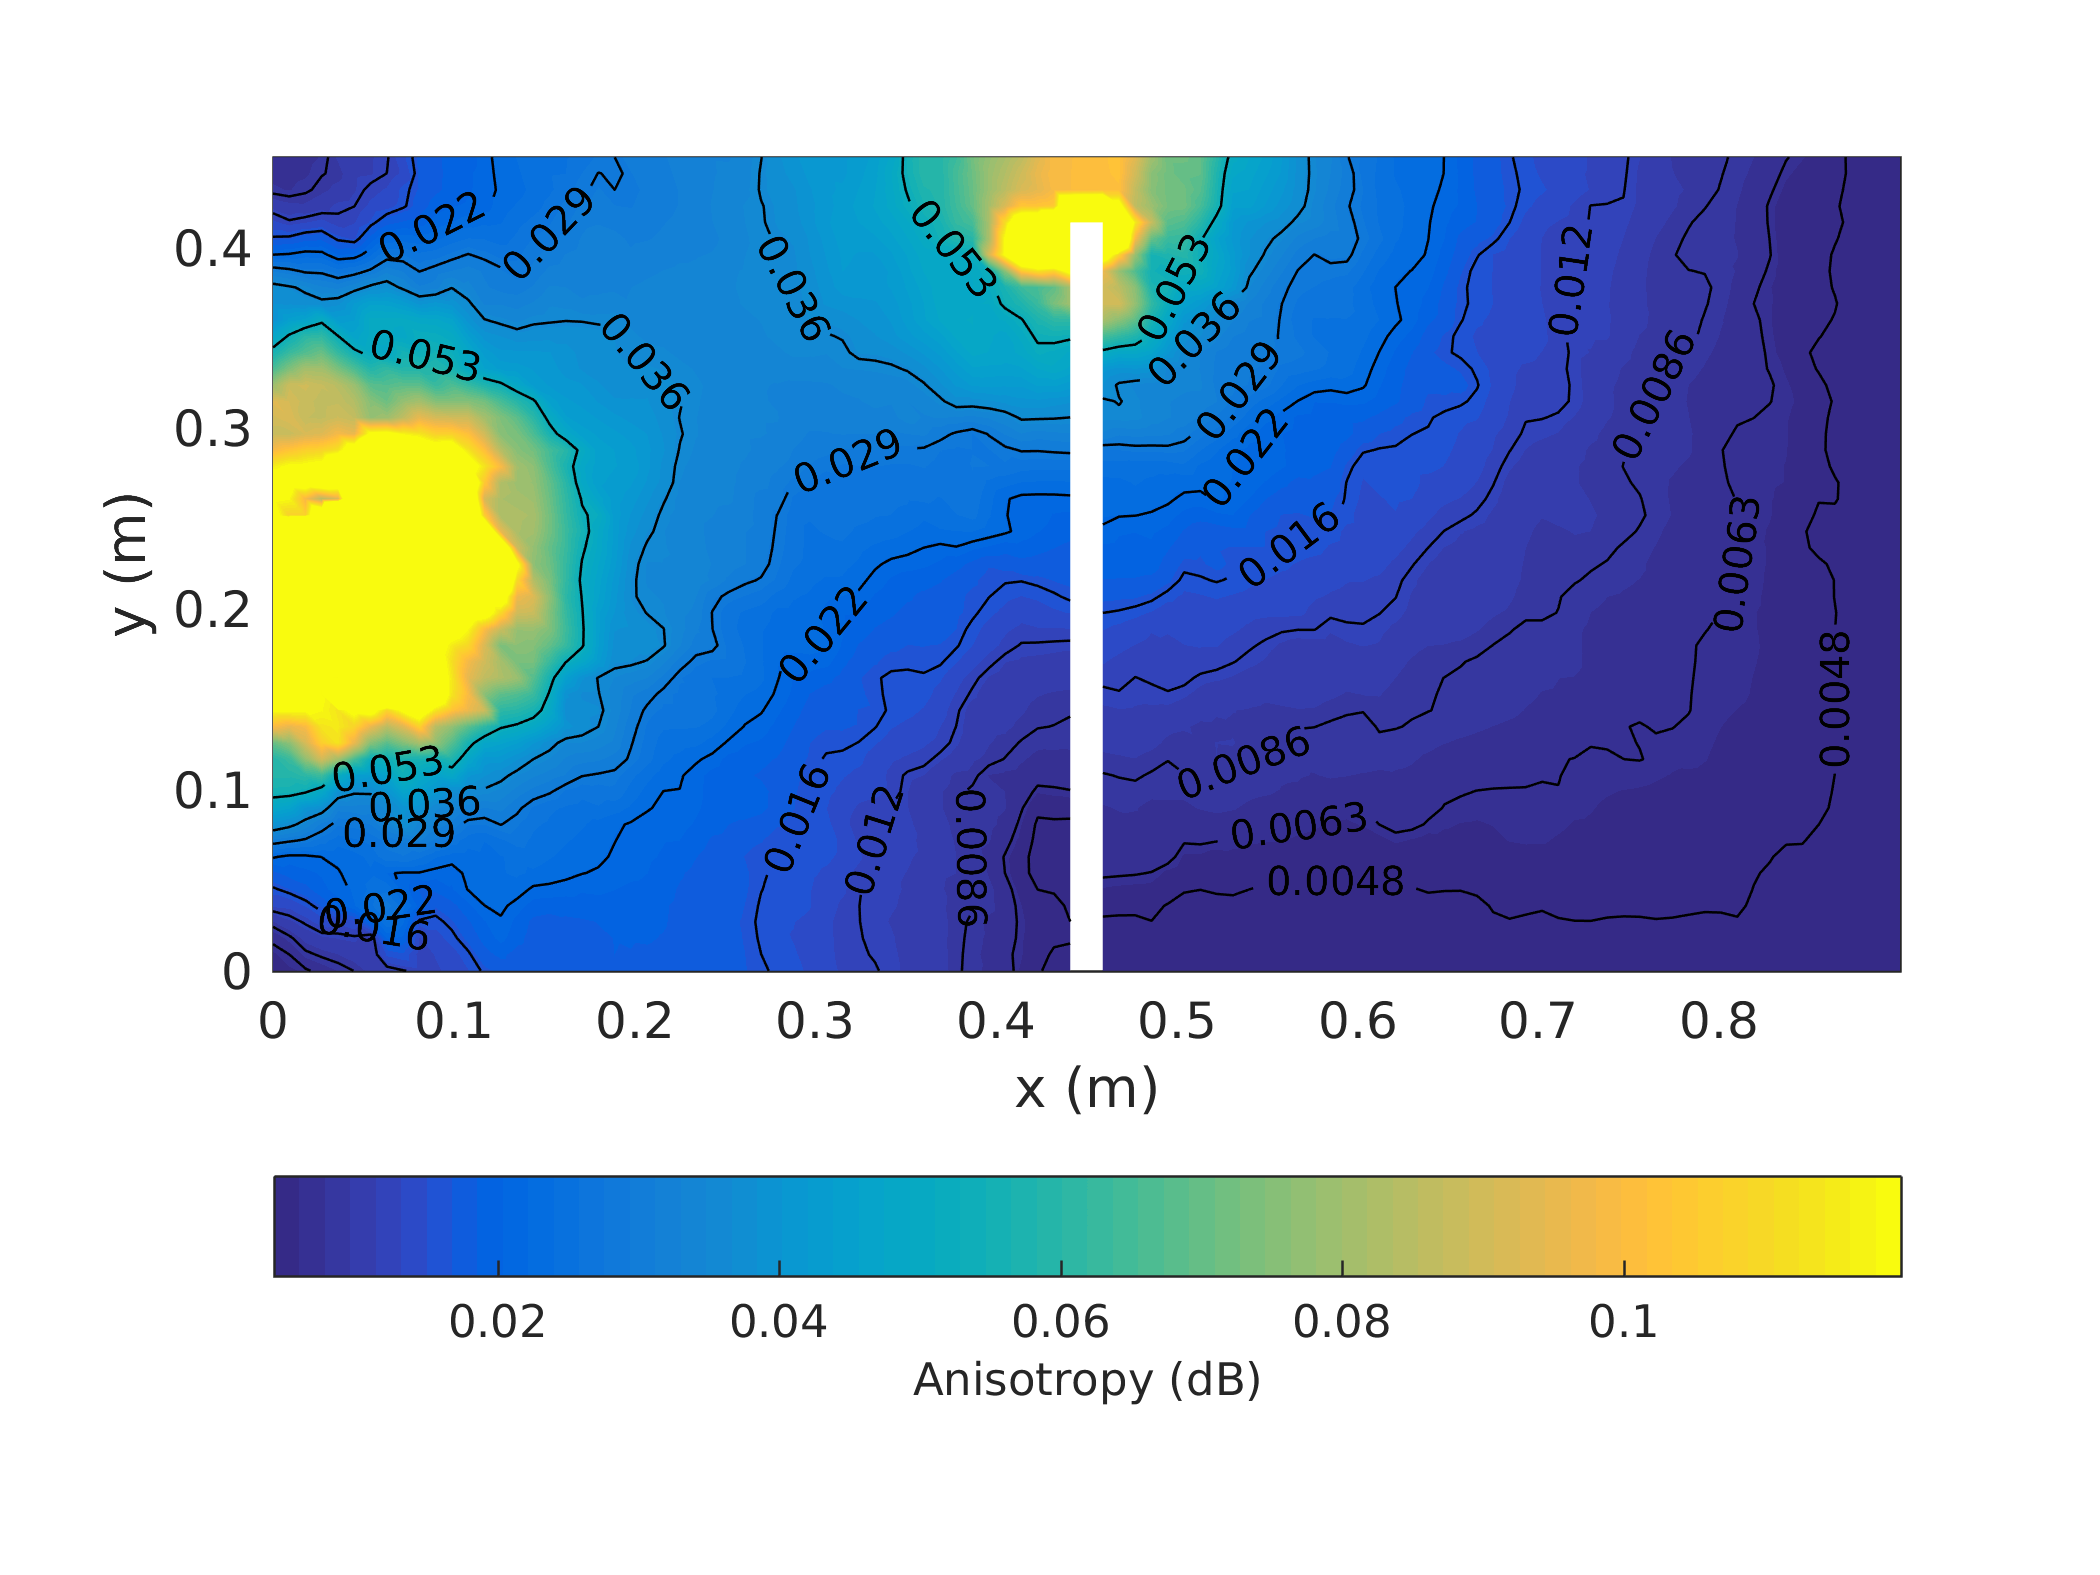
\includegraphics[trim={0 11mm 0 12mm},clip,width=0.52\linewidth]{figures/SDM_3D_DU_EnergyDensityAnisotropyMap}\\
{\footnotesize (c)}\\
\vspace{2mm}
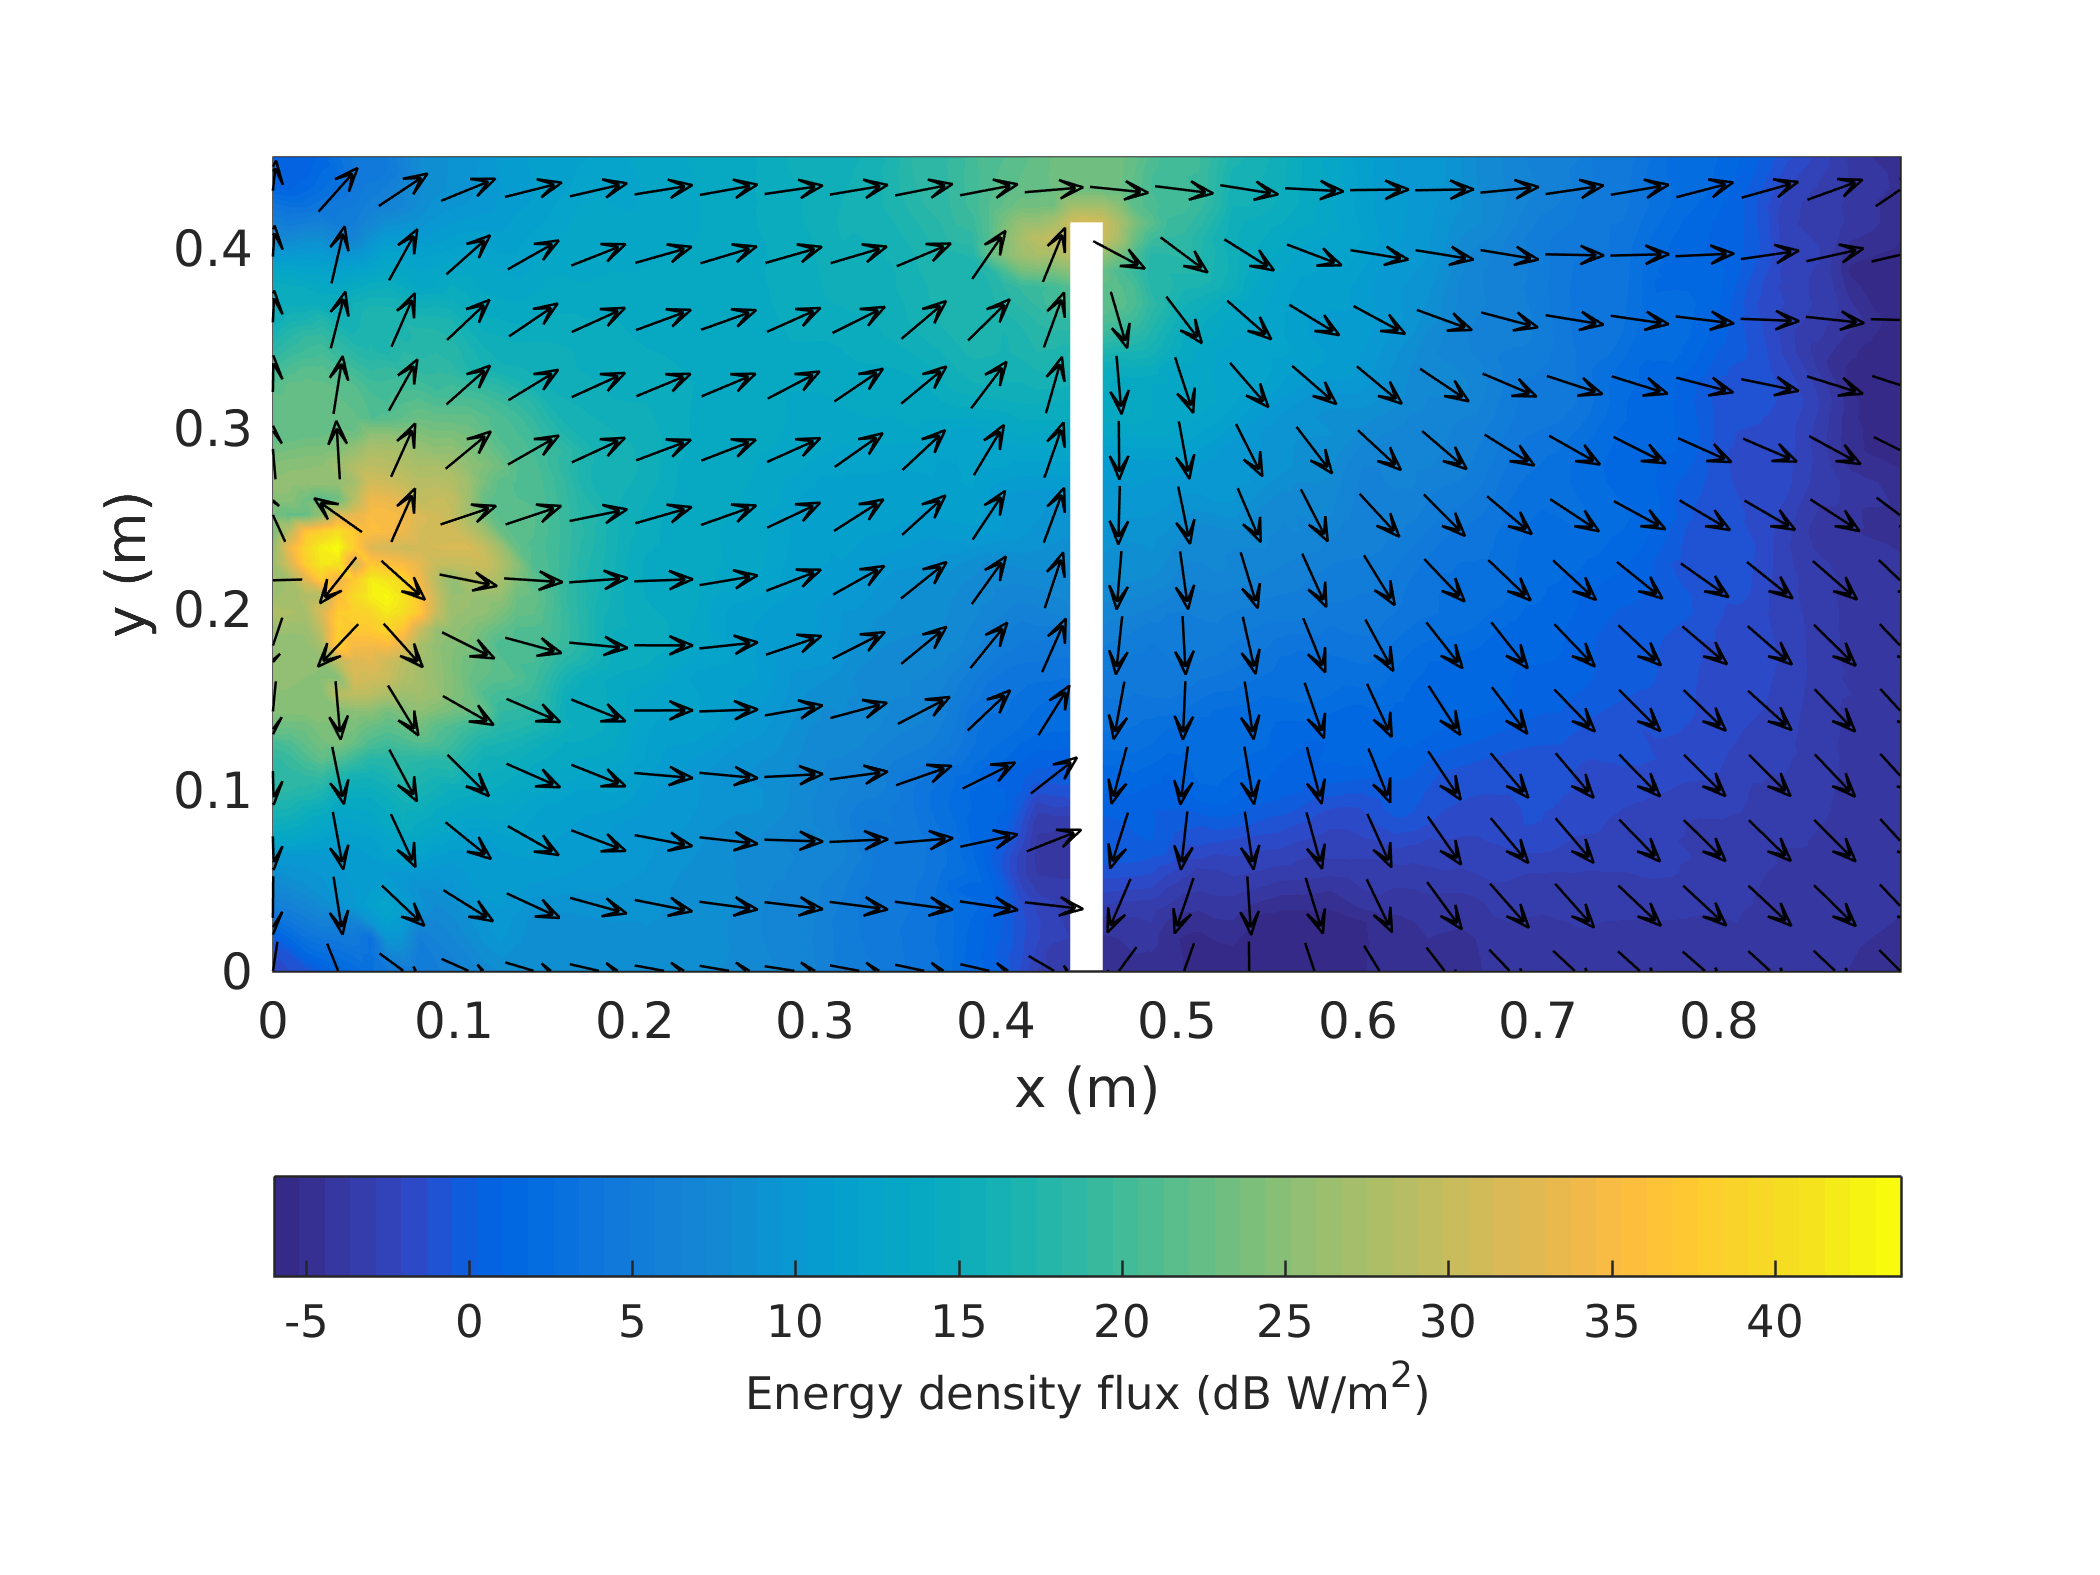
\includegraphics[trim={0 11mm 0 12mm},clip,width=0.52\linewidth]{figures/SDM_3D_DU_EnergyDensityFluxMap}\\
{\footnotesize (d)}\\
\vspace{-2mm}
\caption{\label{fg:partemptysdm_maps} Single domain 3D EDM maps in the $z$-normal plane at the half height of the cavity for the 
unloaded partitioned cavity: (a) Power density; (b) Energy density relative to the homogeneous PWB model;
(c) Anisotropy; (d) Energy density flux.}
\end{center}
\end{figure}

\begin{figure}[hp]
\begin{center}
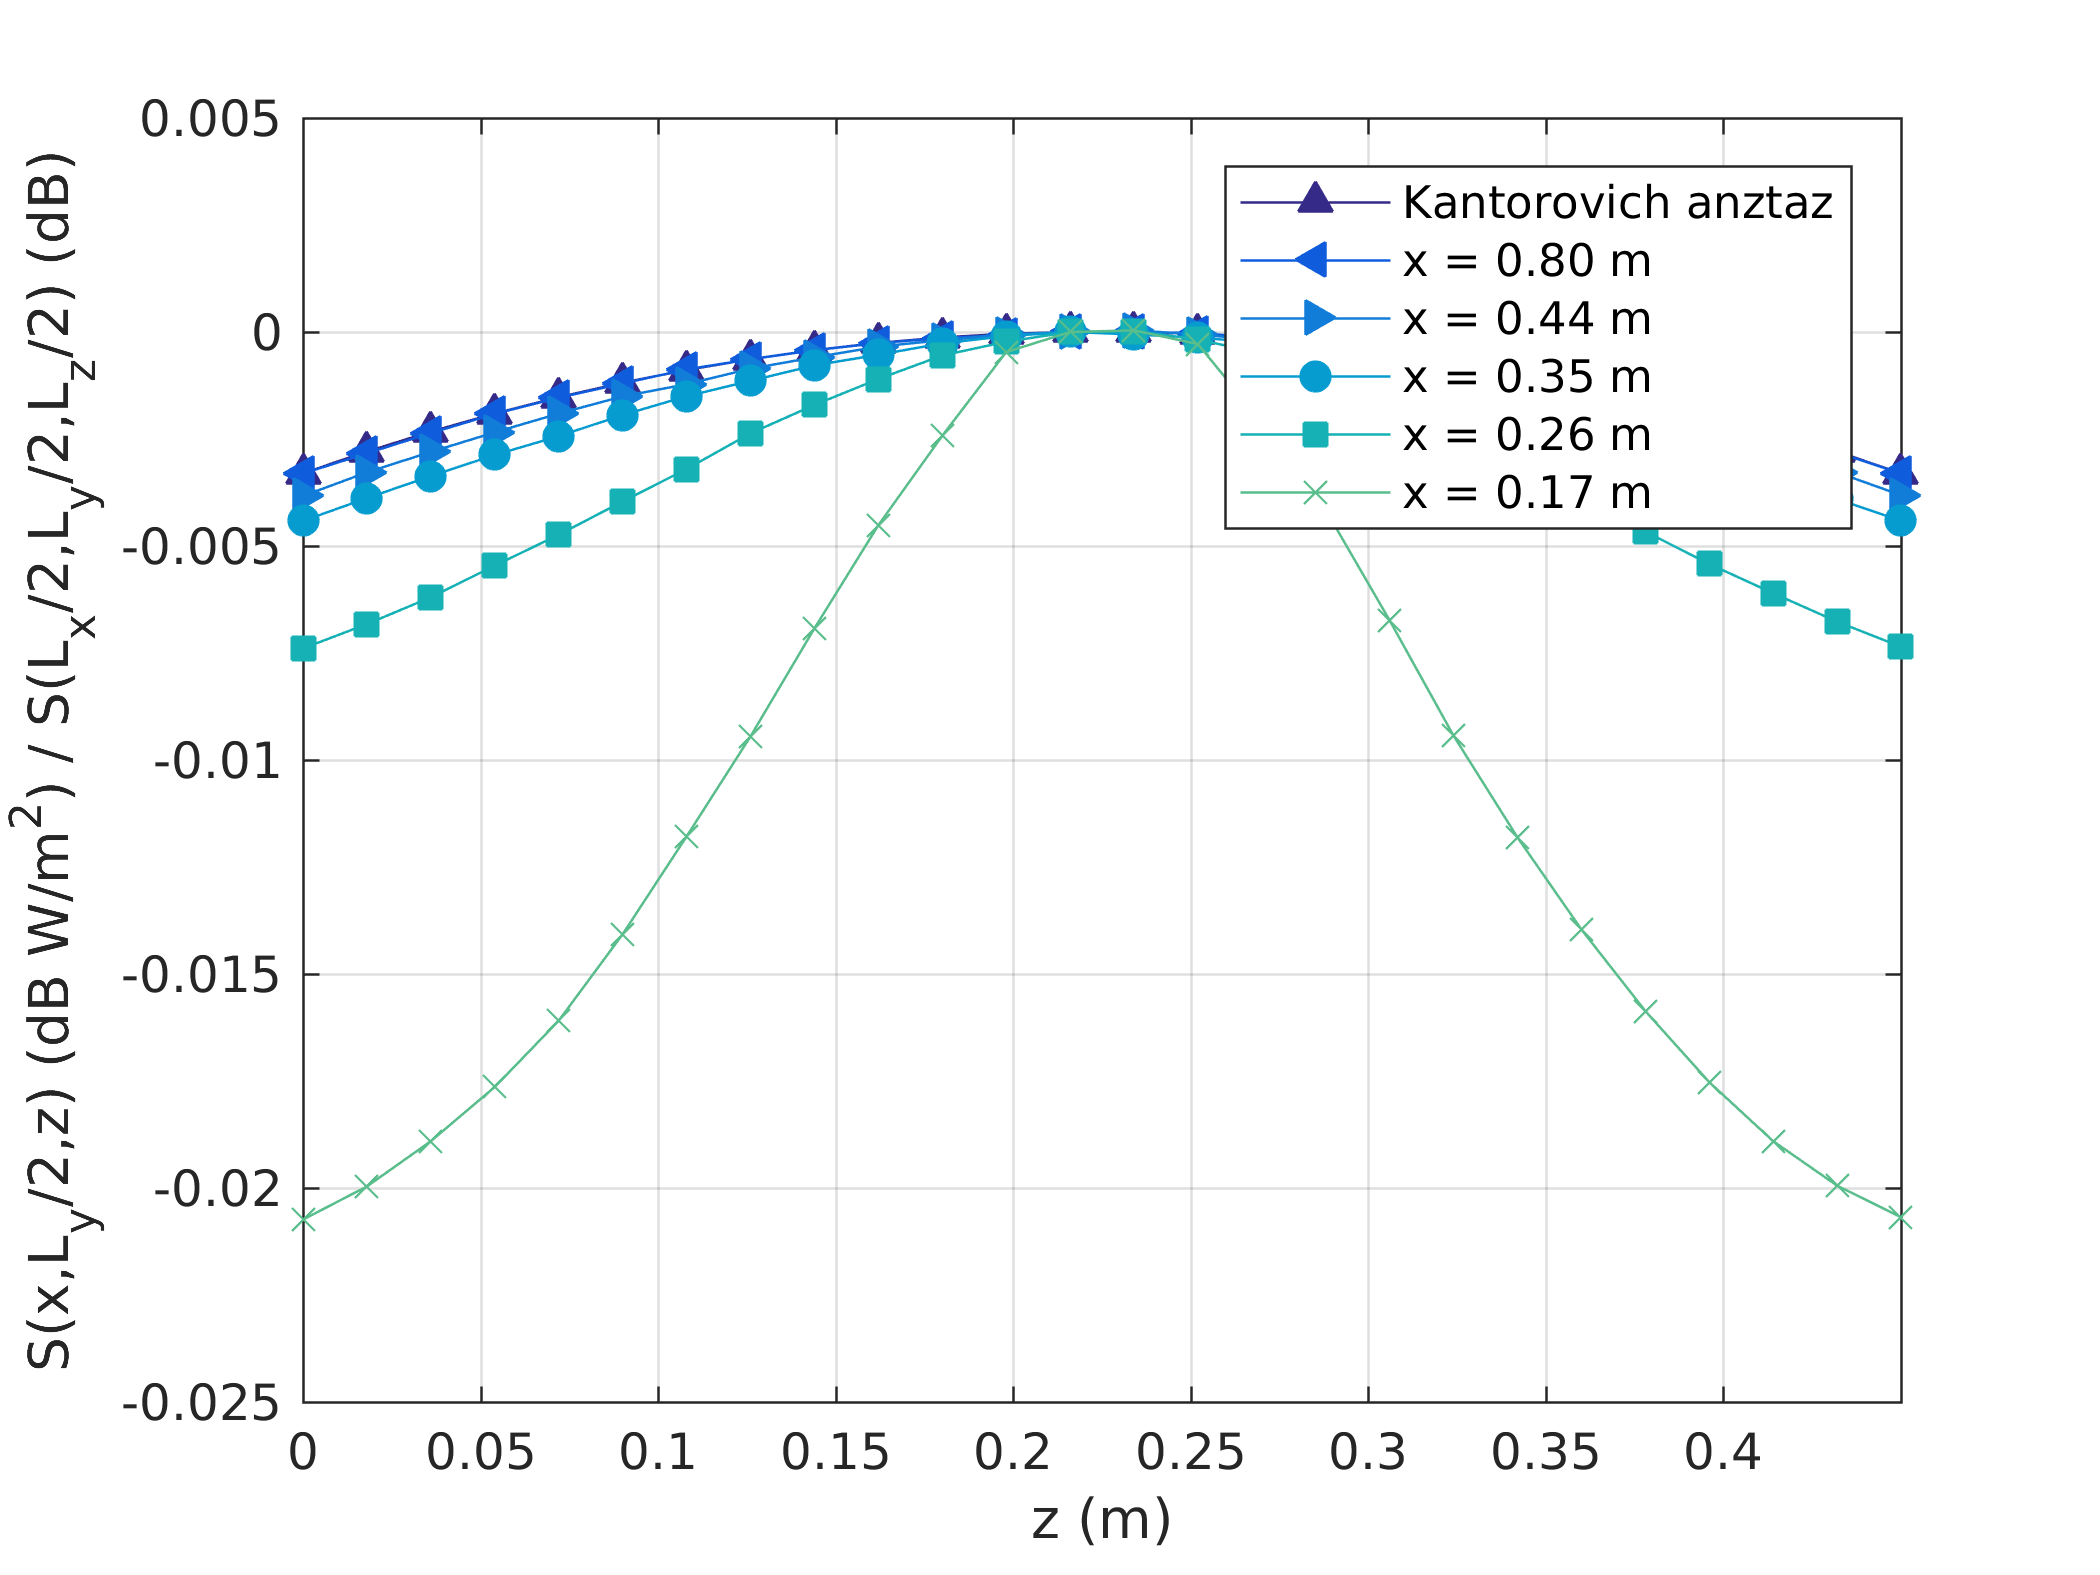
\includegraphics[width=0.6\linewidth]{figures/DDM-EEBC_3D_DU_PowerDensityProfileZ}\\
{\footnotesize (a)}\\
\vspace{2mm}
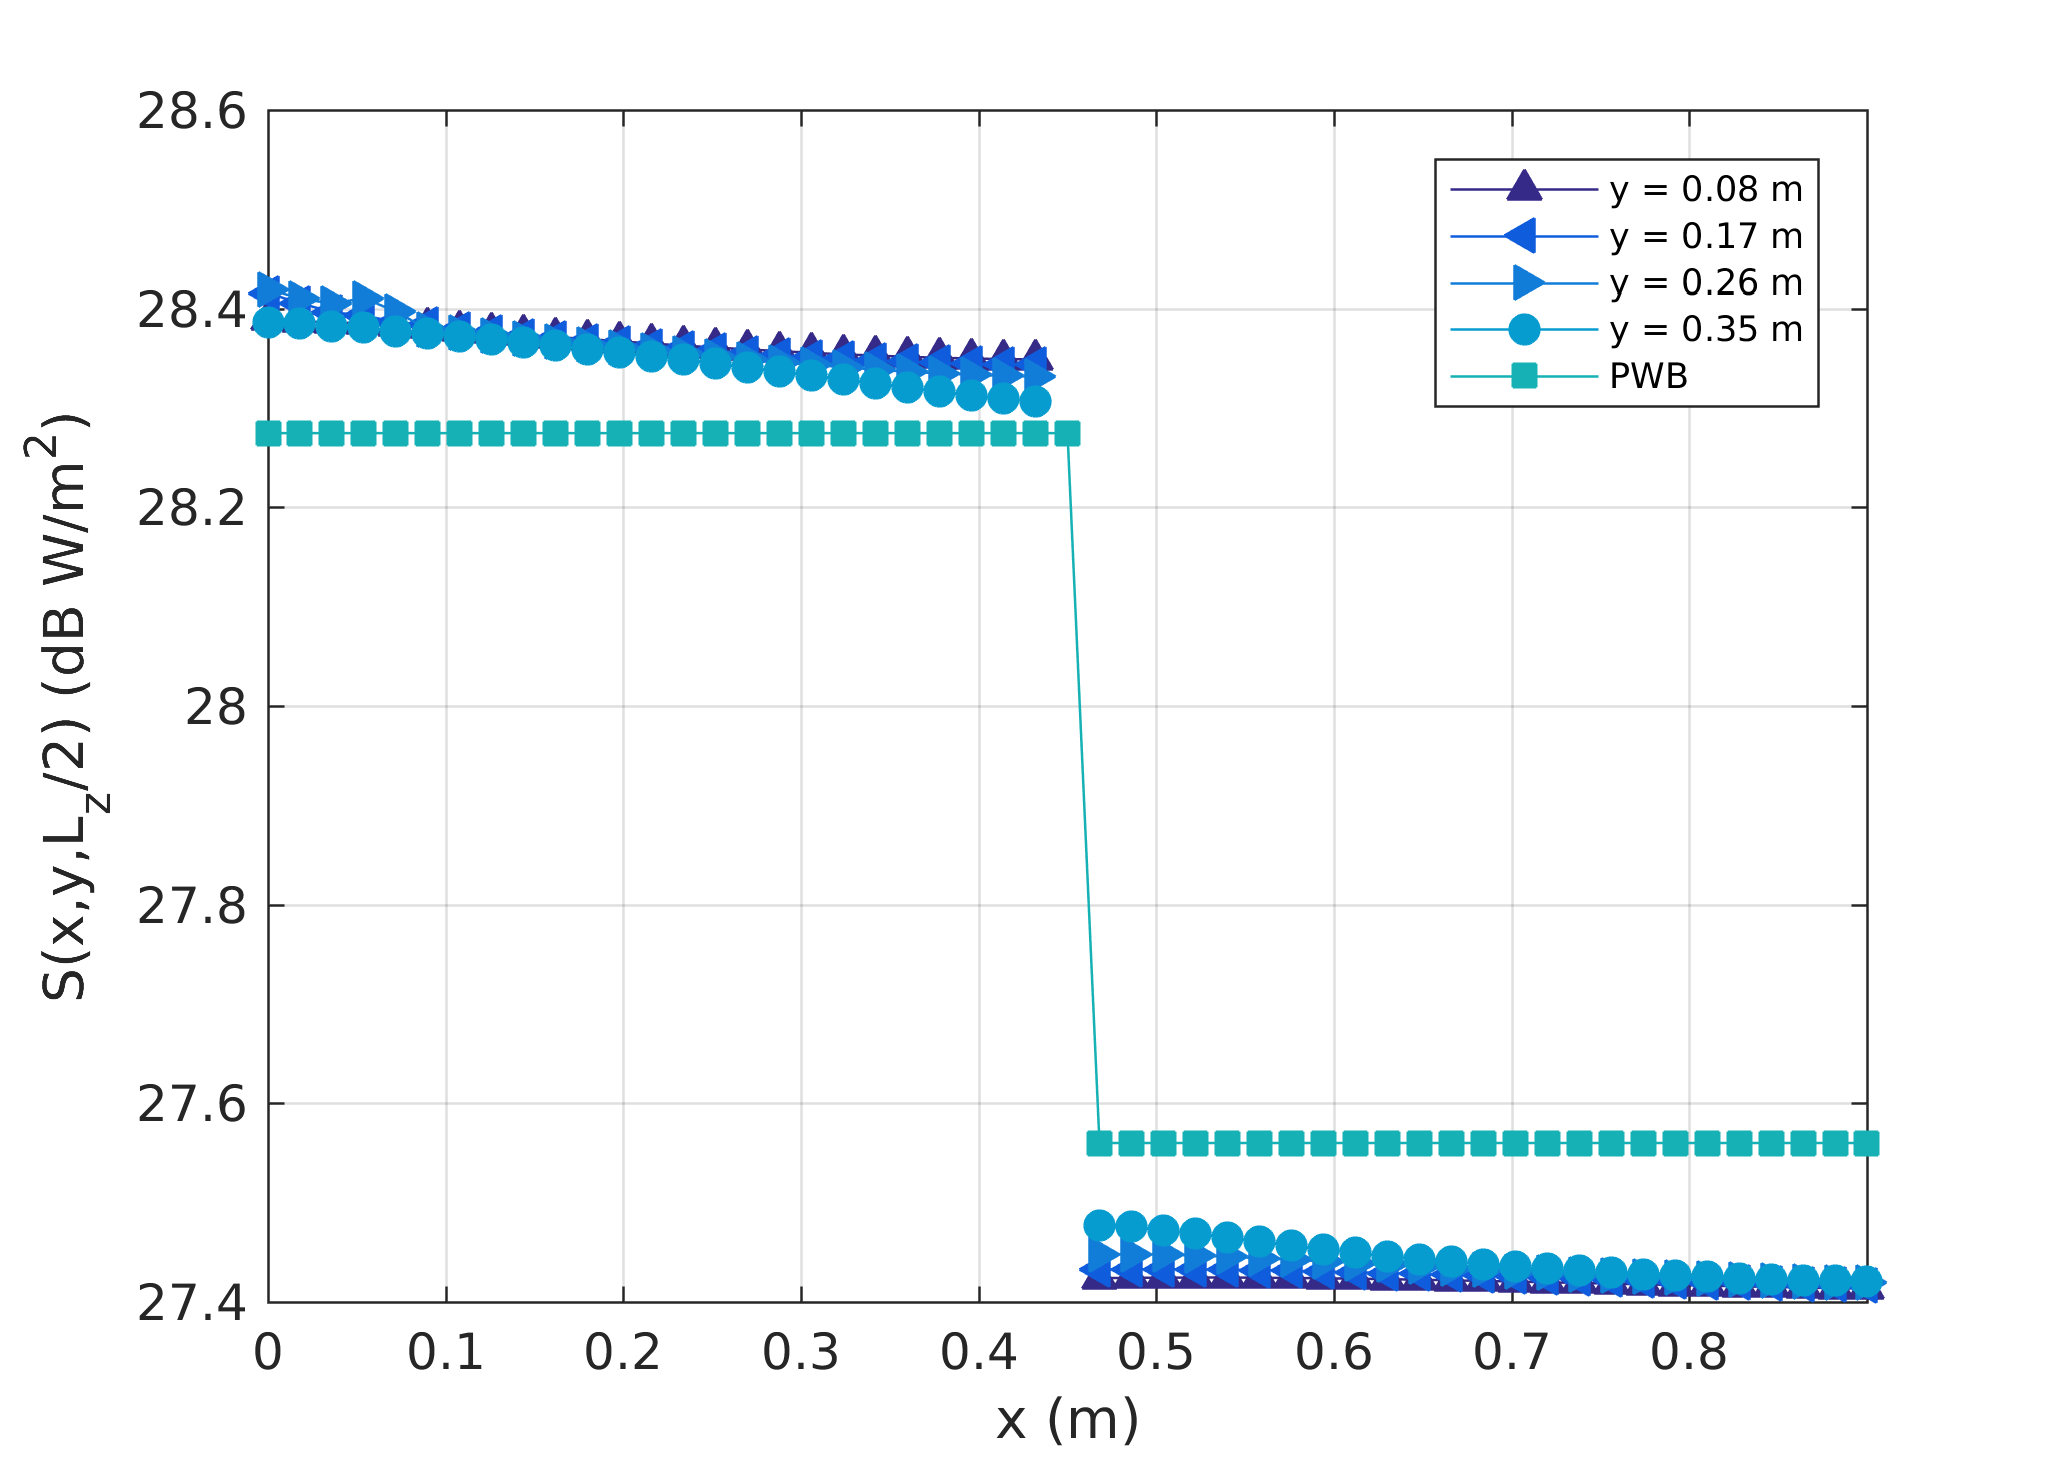
\includegraphics[width=0.6\linewidth]{figures/DDM-EEBC_3D_DU_PowerDensityProfileX}\\
{\footnotesize (b)}\\
\vspace{2mm}
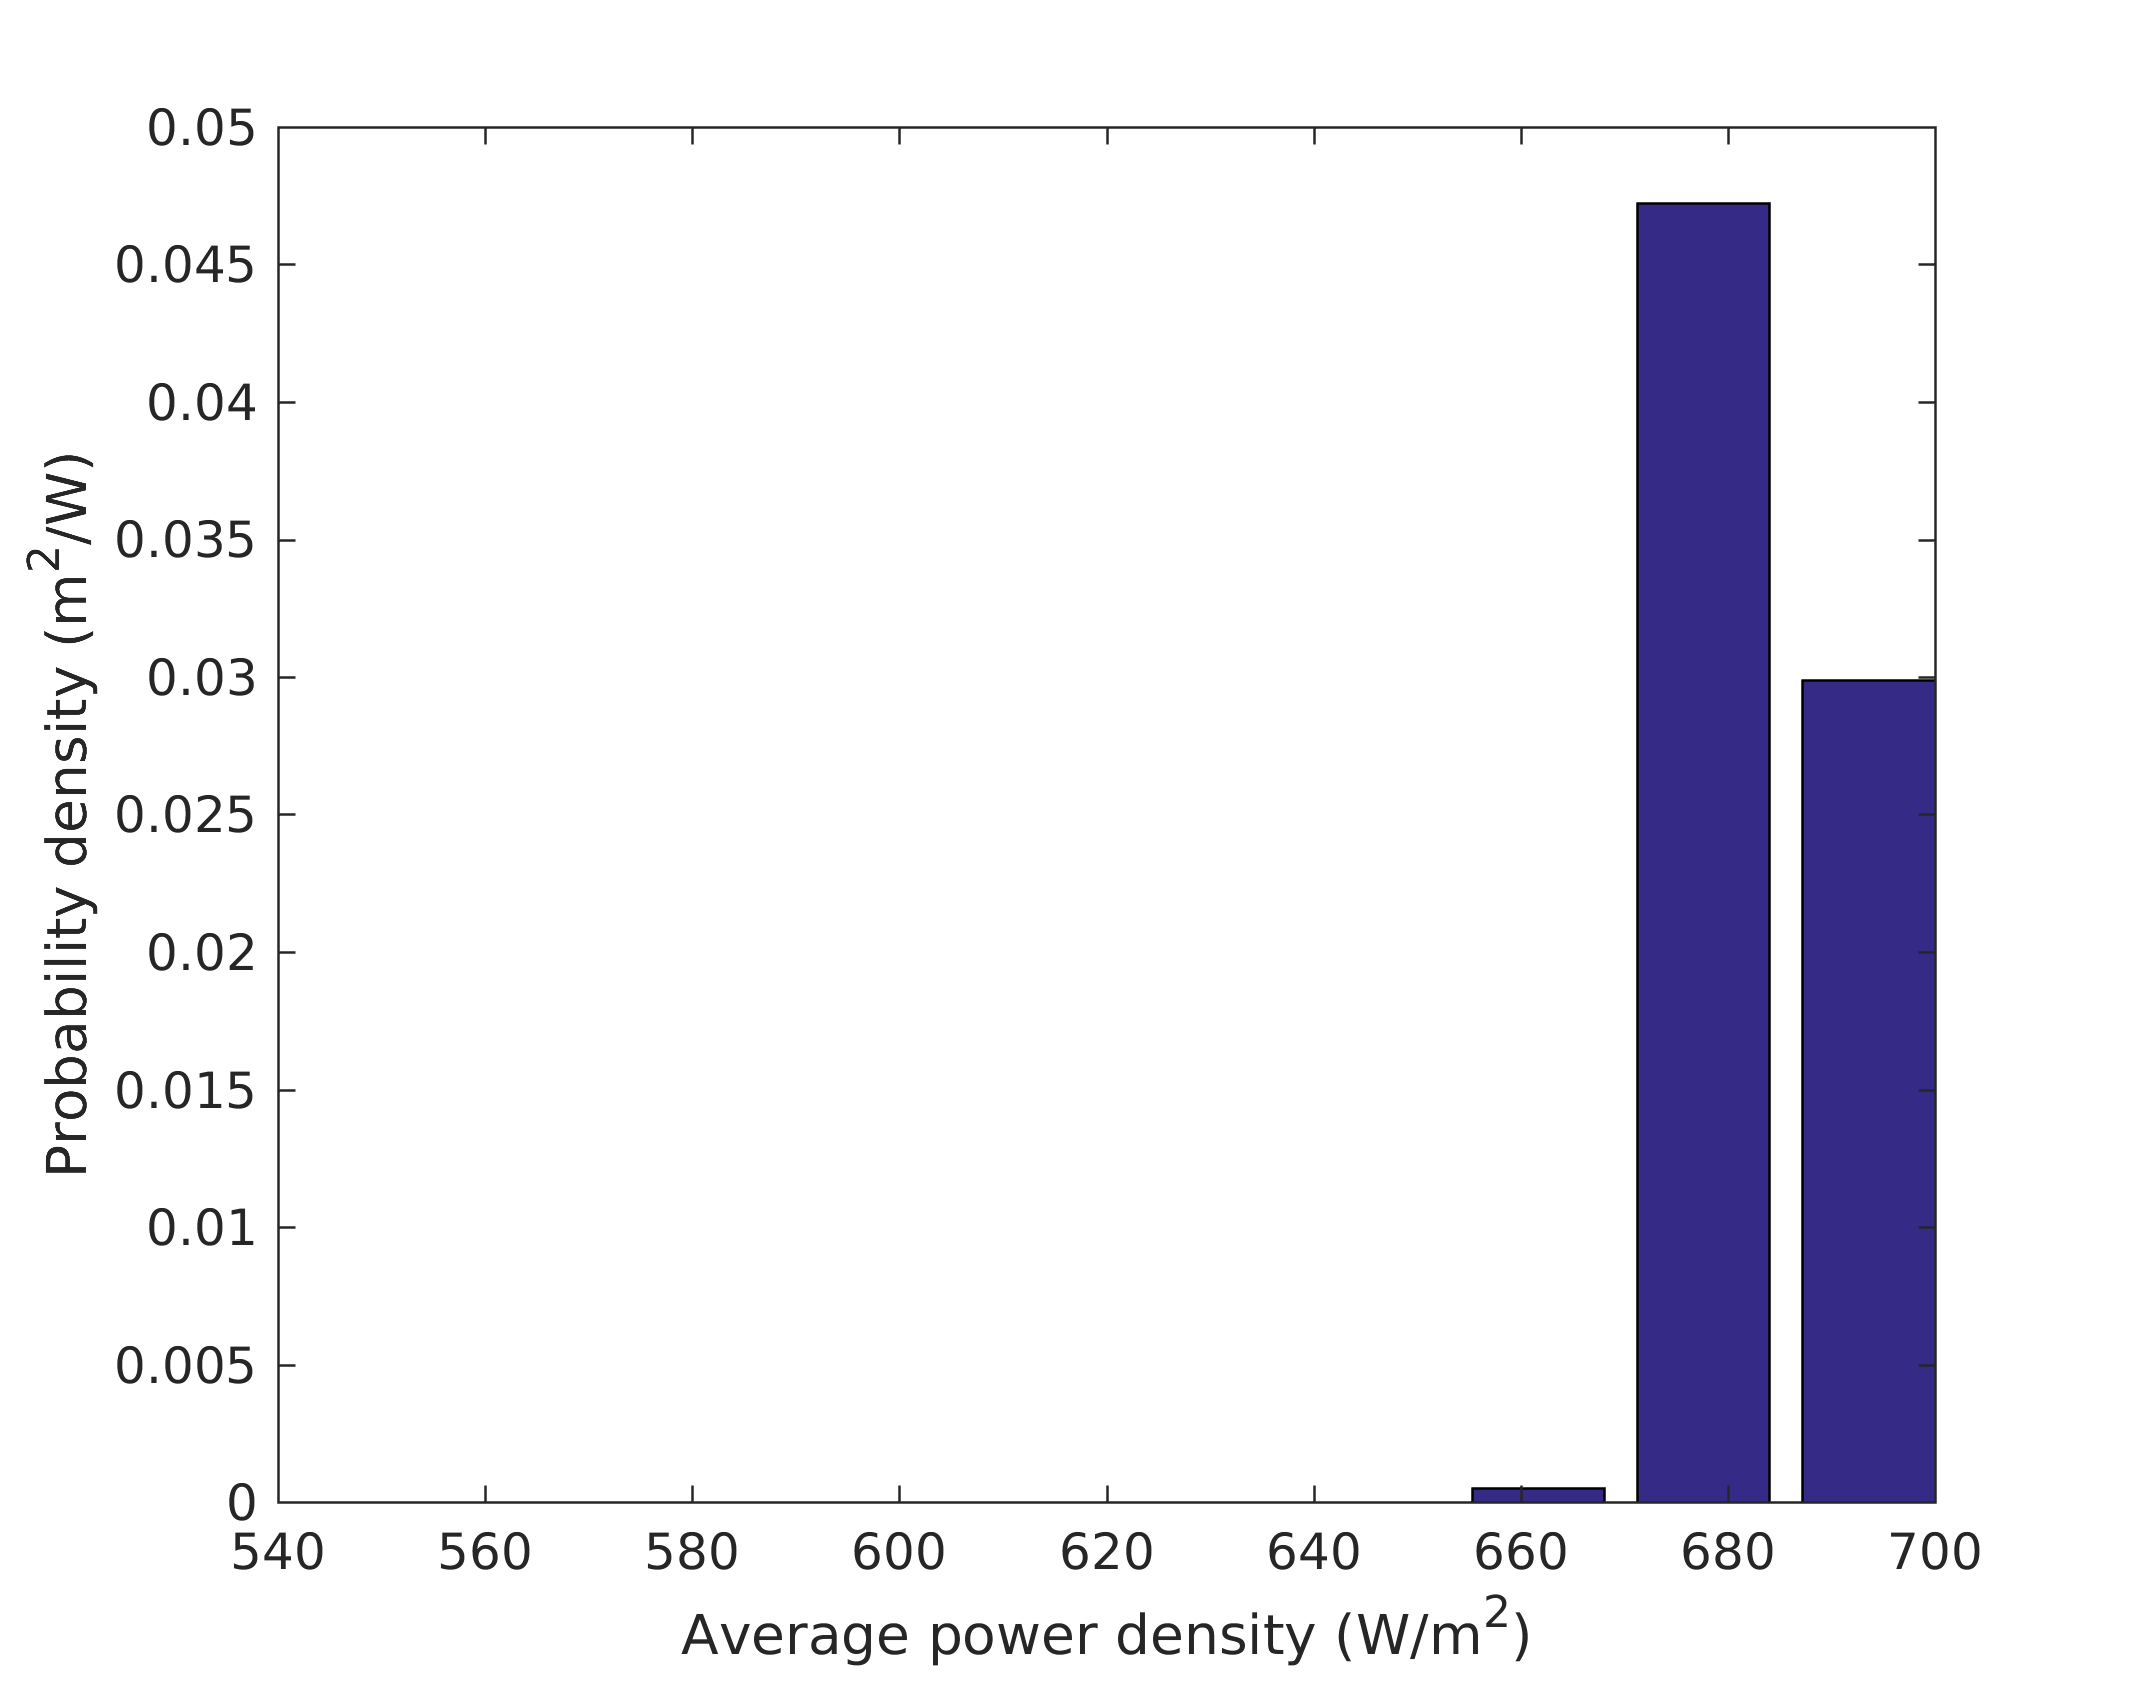
\includegraphics[width=0.45\linewidth]{figures/DDM-EEBC_3D_DU_PowerDensityPDF1}
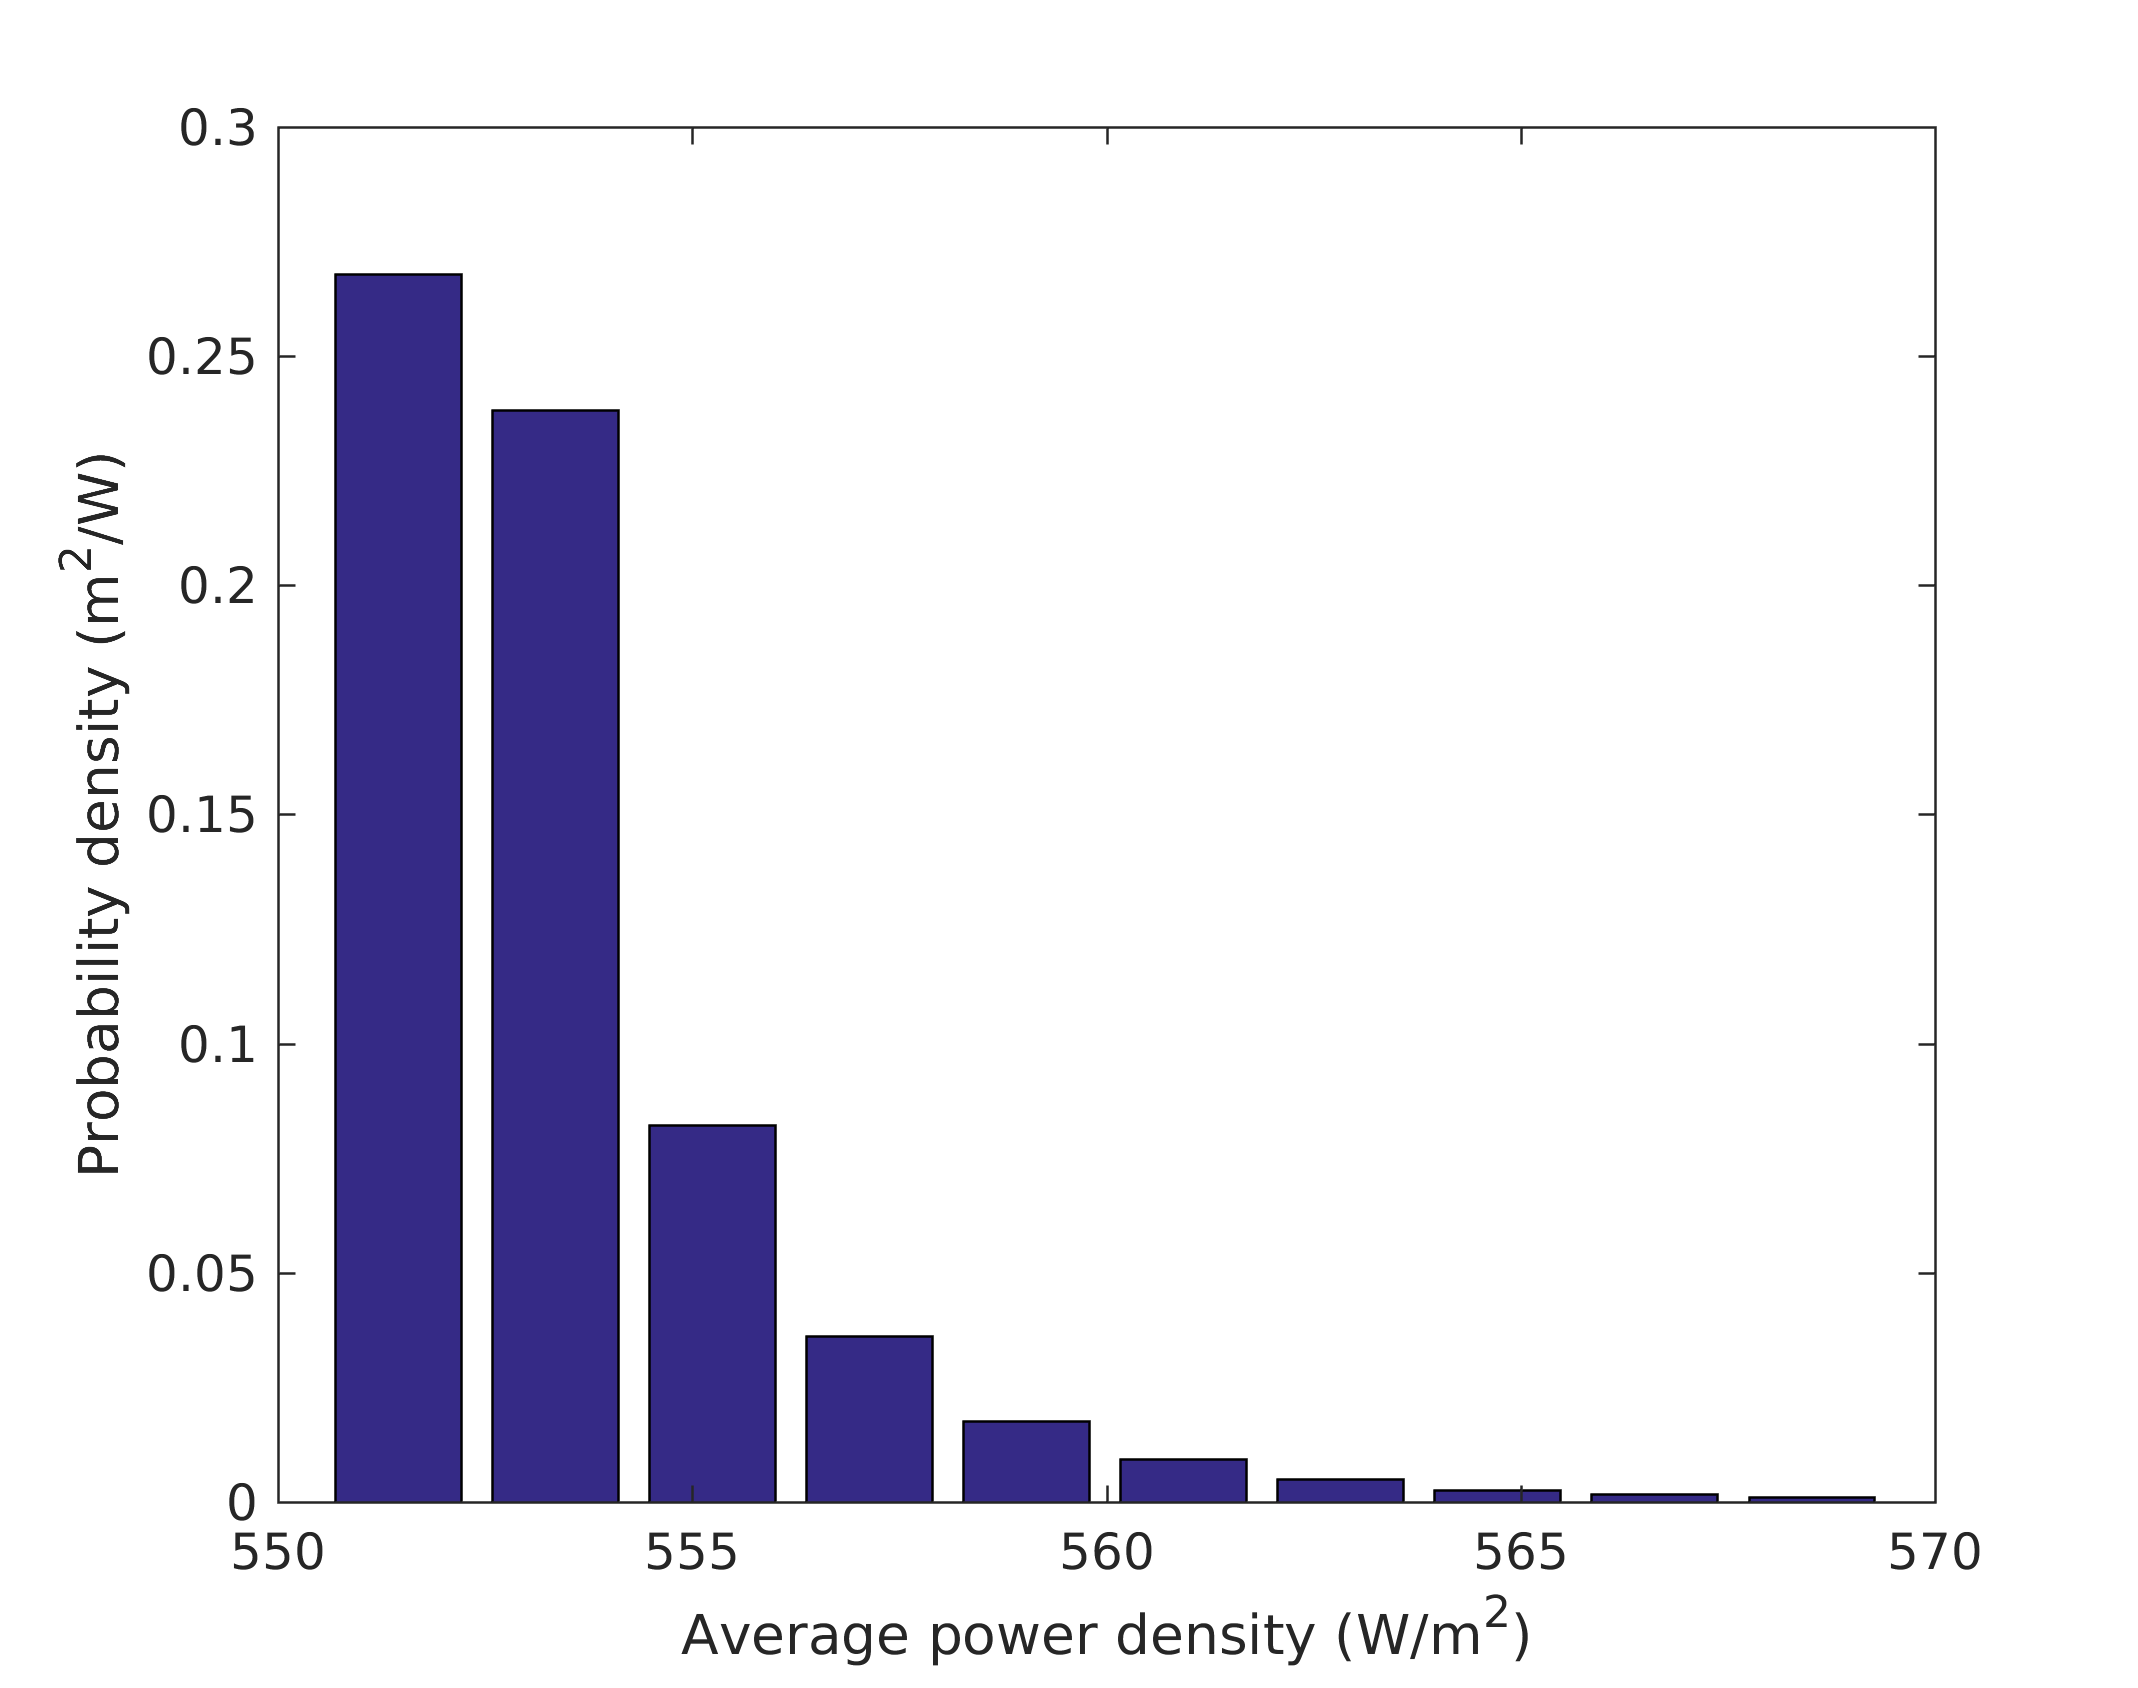
\includegraphics[width=0.45\linewidth]{figures/DDM-EEBC_3D_DU_PowerDensityPDF2}
\\
{\footnotesize (c)}\\
\vspace{-2mm}
\caption{\label{fg:partemptyddm_profs} Dual domain EEBC EDM of the unloaded partitioned cavity: (a) Normalised vertical profile of the power density; 
(b) Power density profile in the $x$-direction along the cavity centre; (c) PDF of the power density in the source cavity (left) and coupled cavity (right).}
\end{center}
\end{figure}

\begin{figure}[hp]
\begin{center}
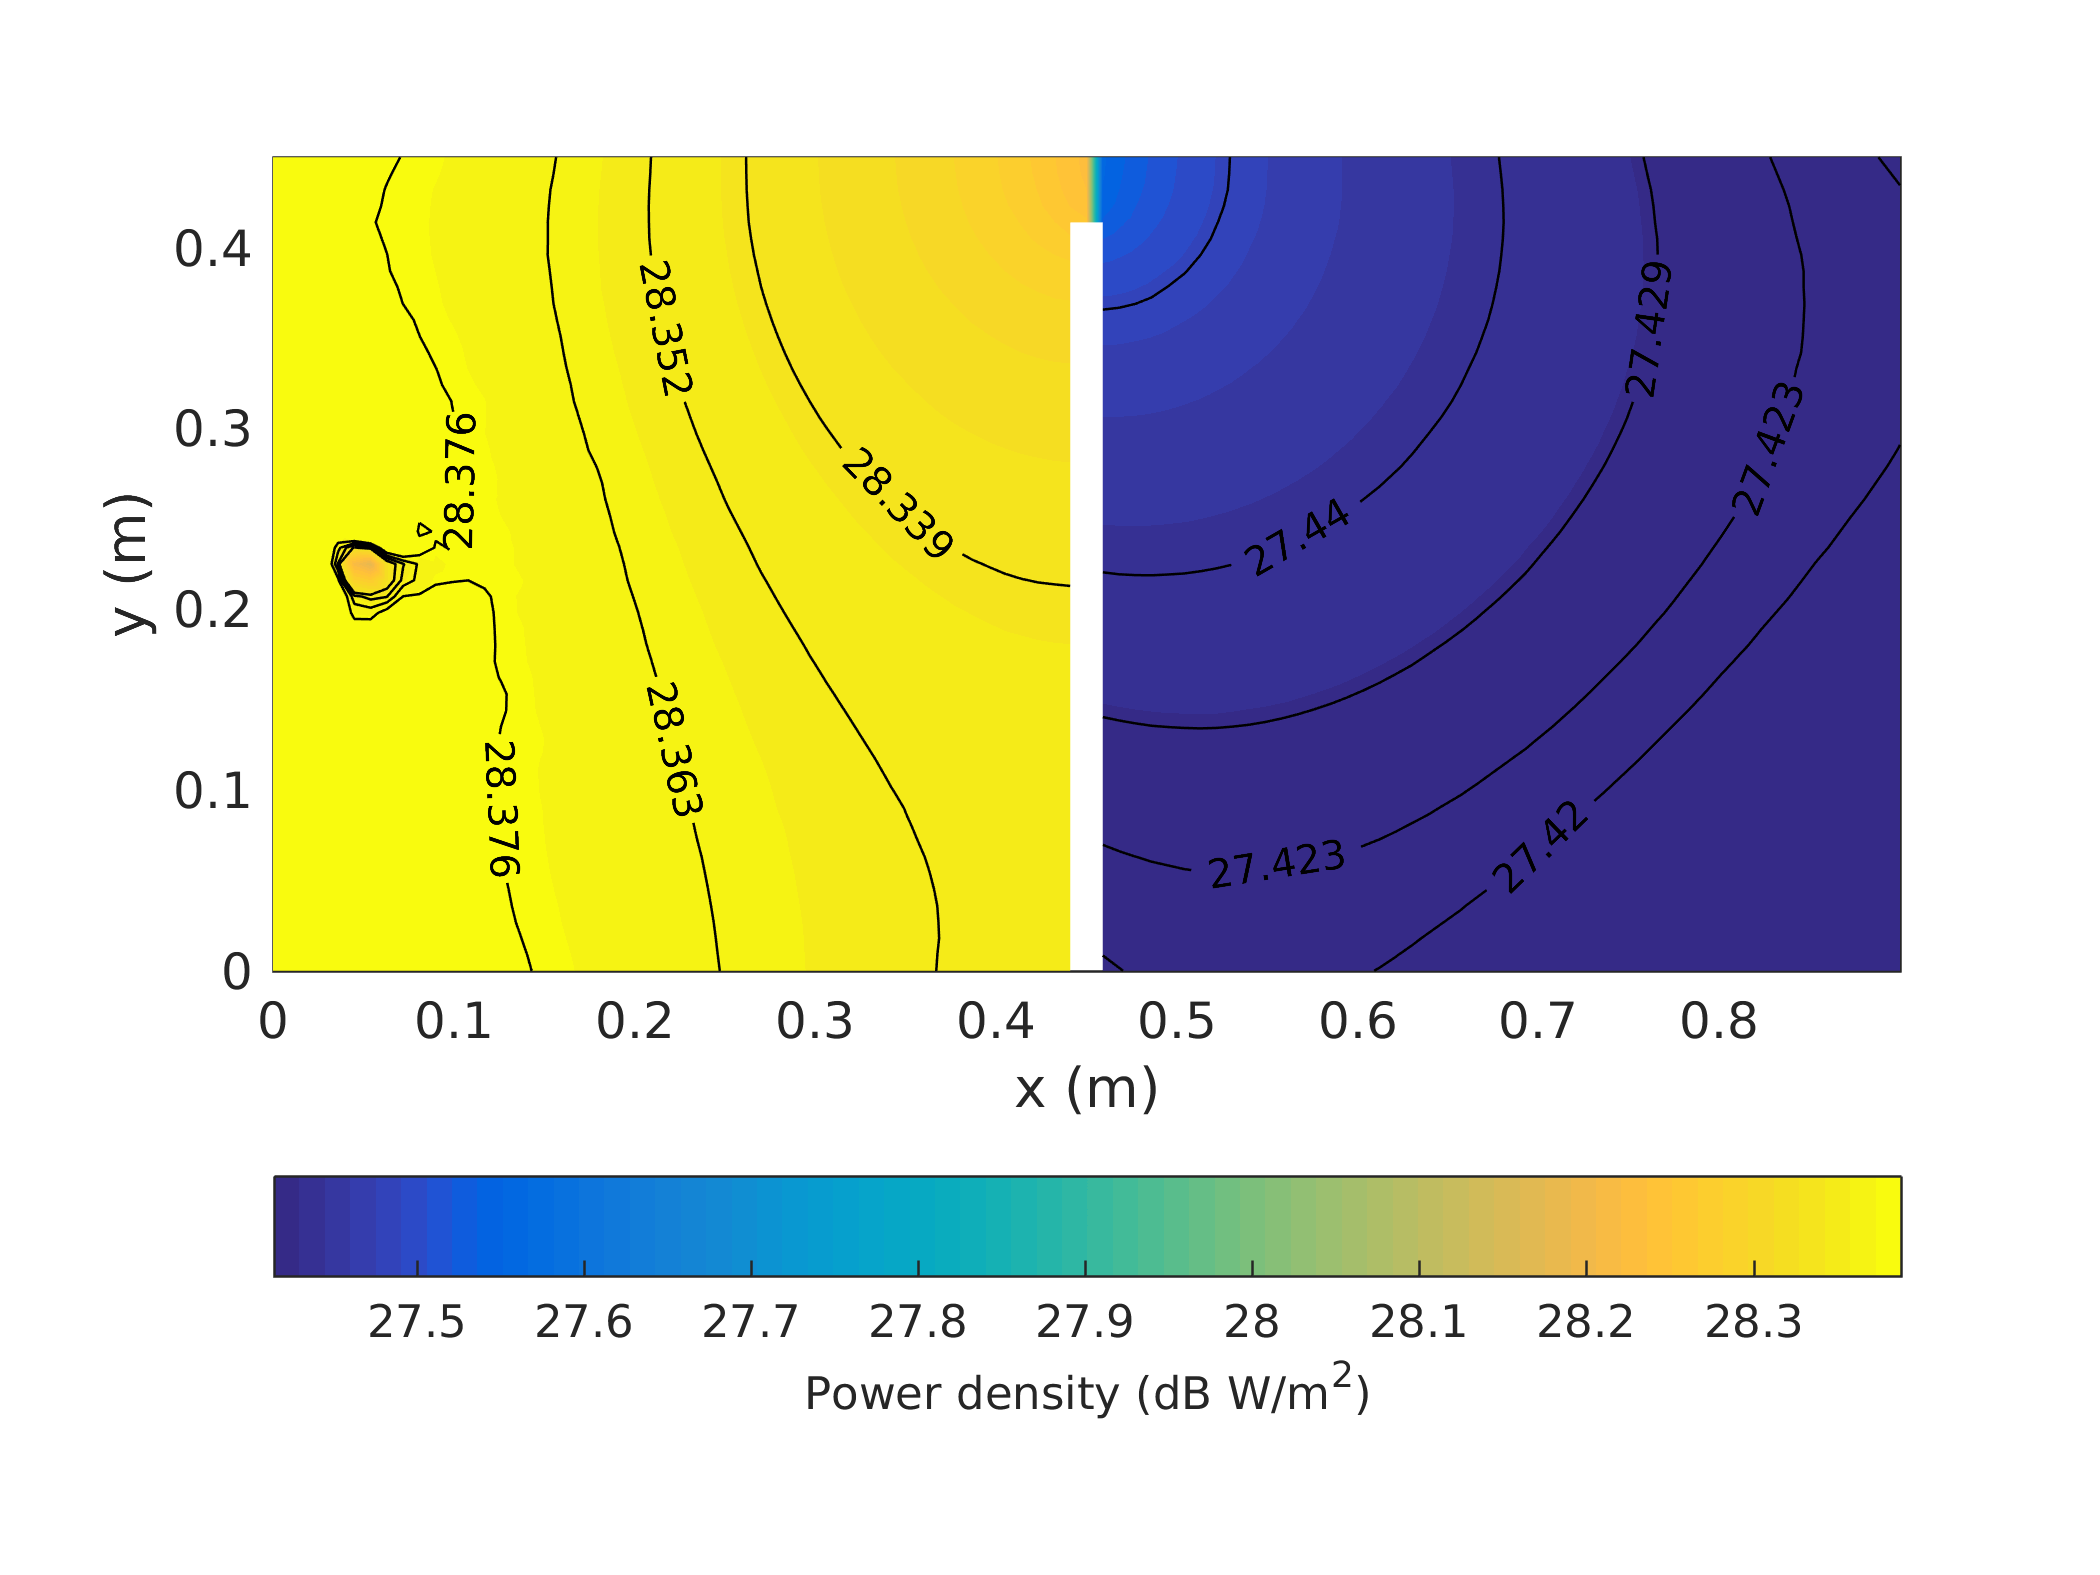
\includegraphics[trim={0 8mm 0 12mm},clip,width=0.52\linewidth]{figures/DDM-EEBC_3D_DU_PowerDensityMap}\\
{\footnotesize (a)}\\
\vspace{2mm}
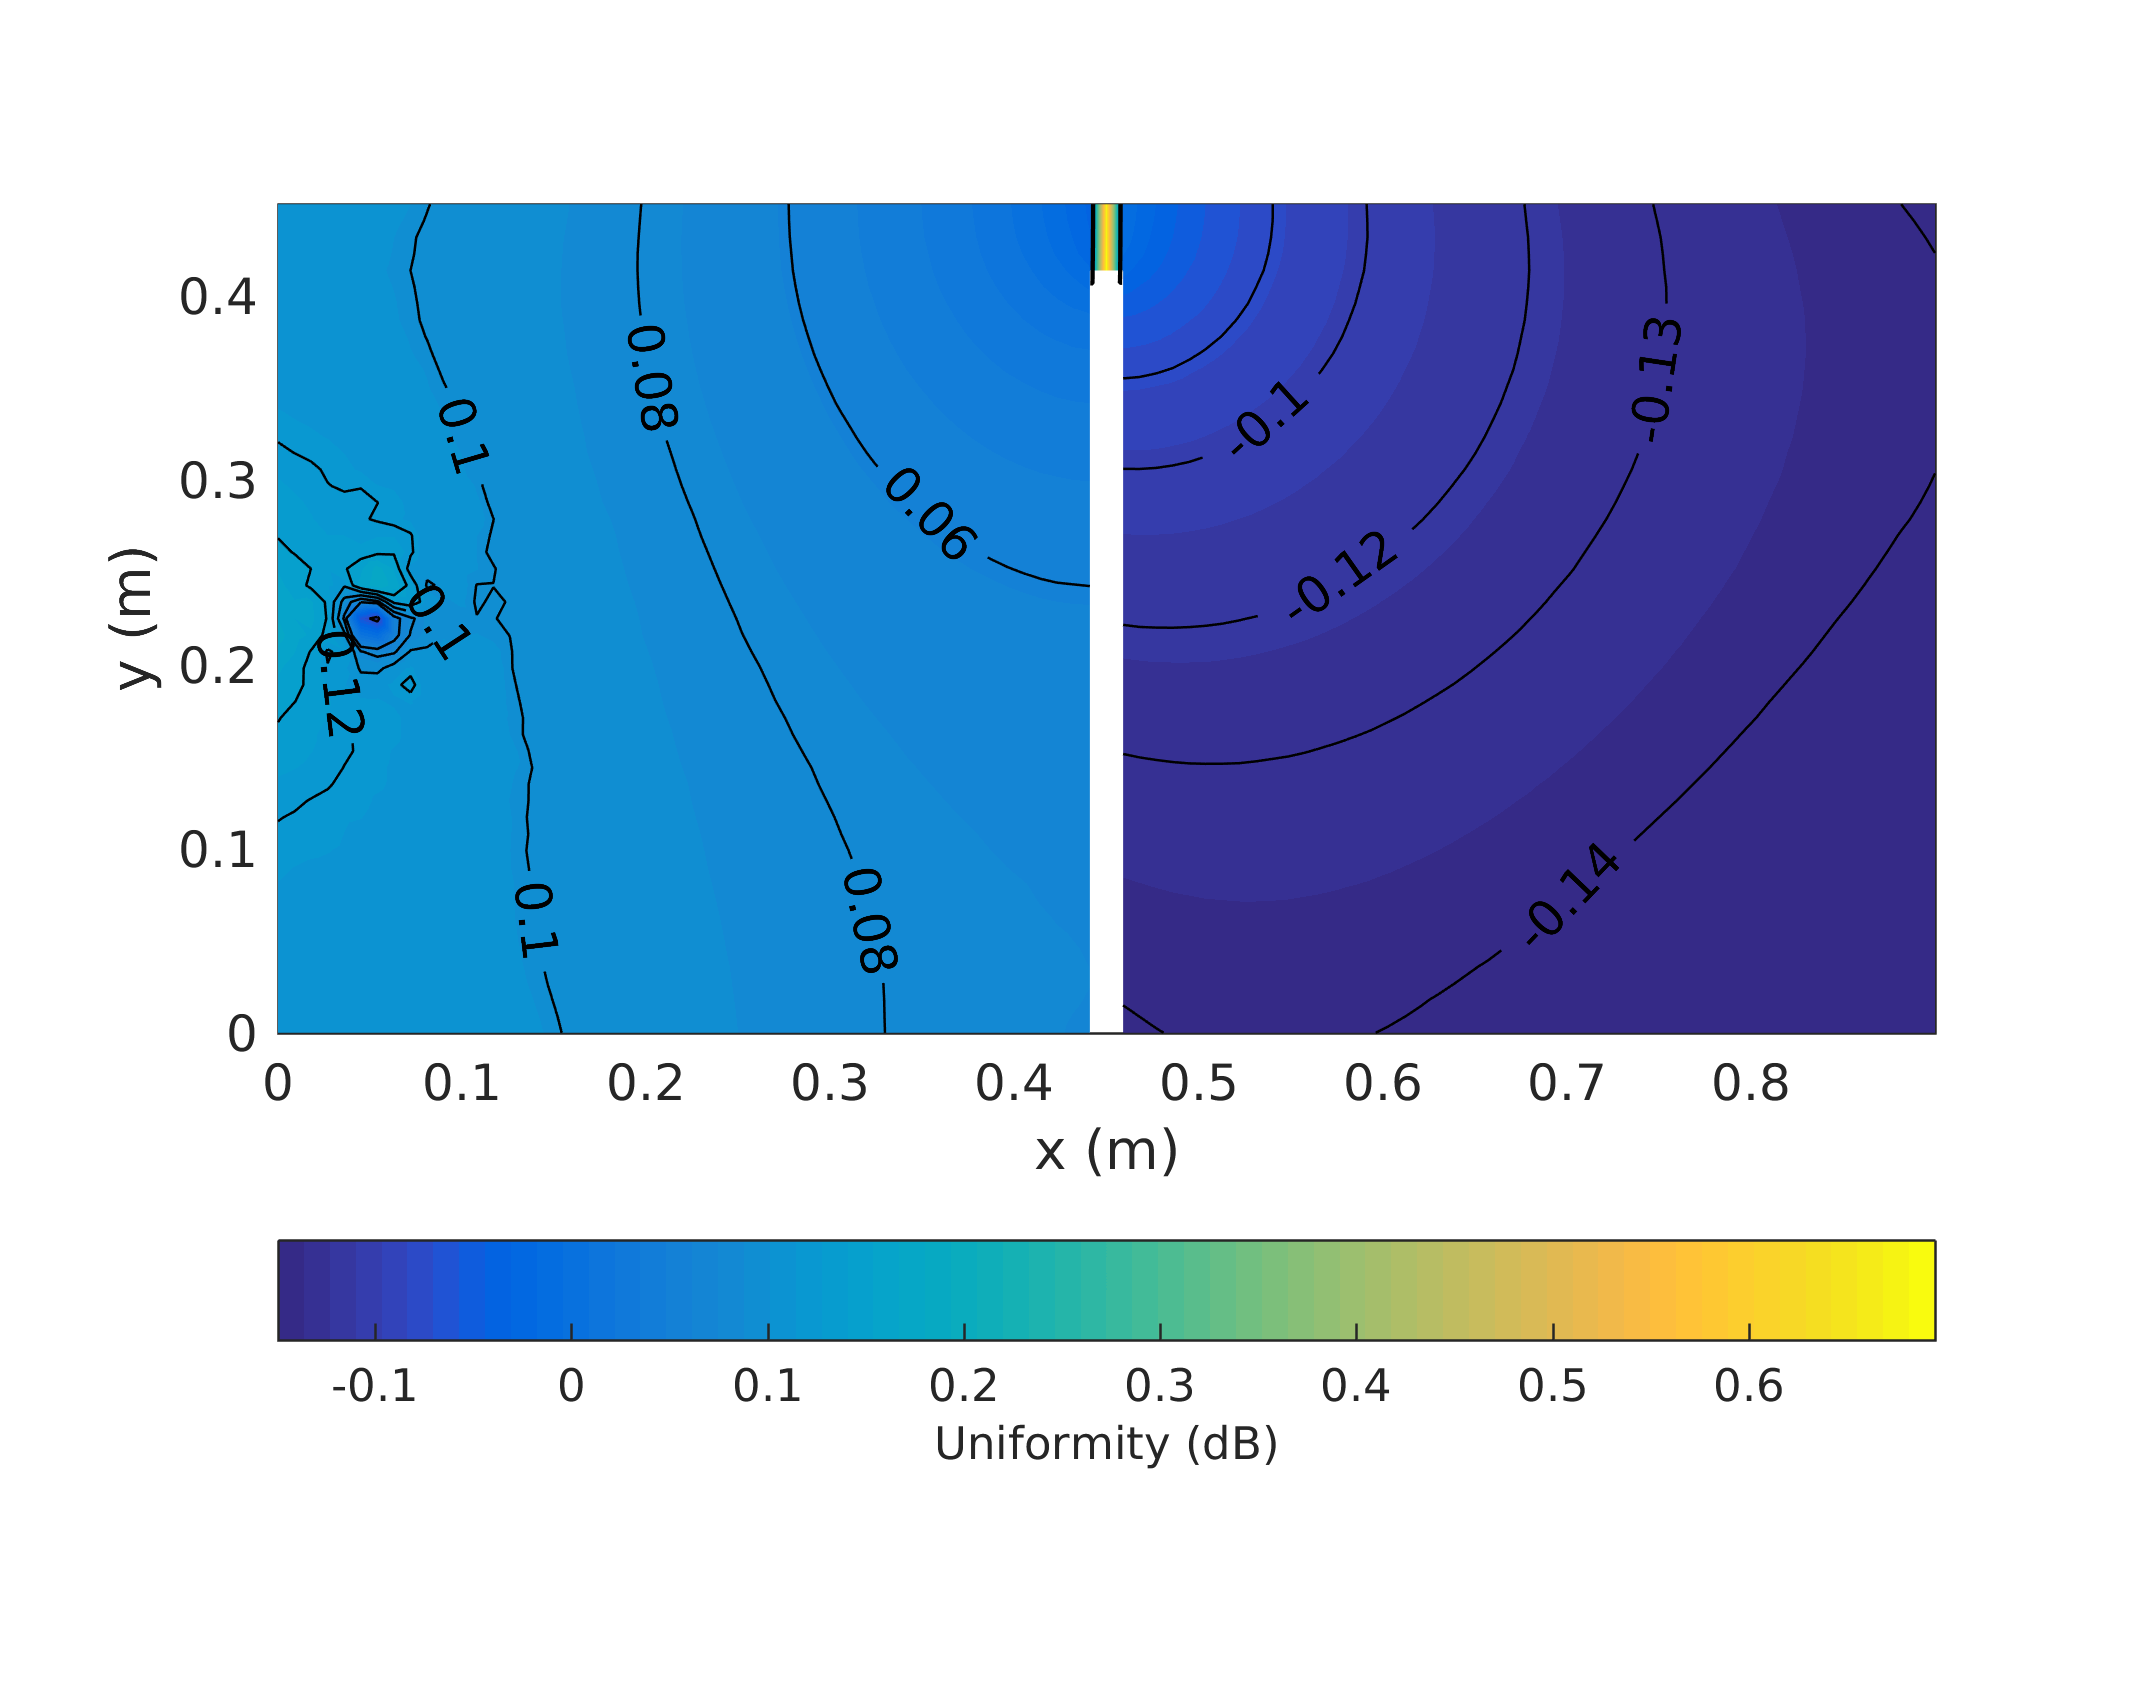
\includegraphics[trim={0 8mm 0 12mm},clip,width=0.52\linewidth]{figures/DDM-EEBC_3D_DU_EnergyDensityUniformityMap}\\
{\footnotesize (b)}\\
\vspace{2mm}
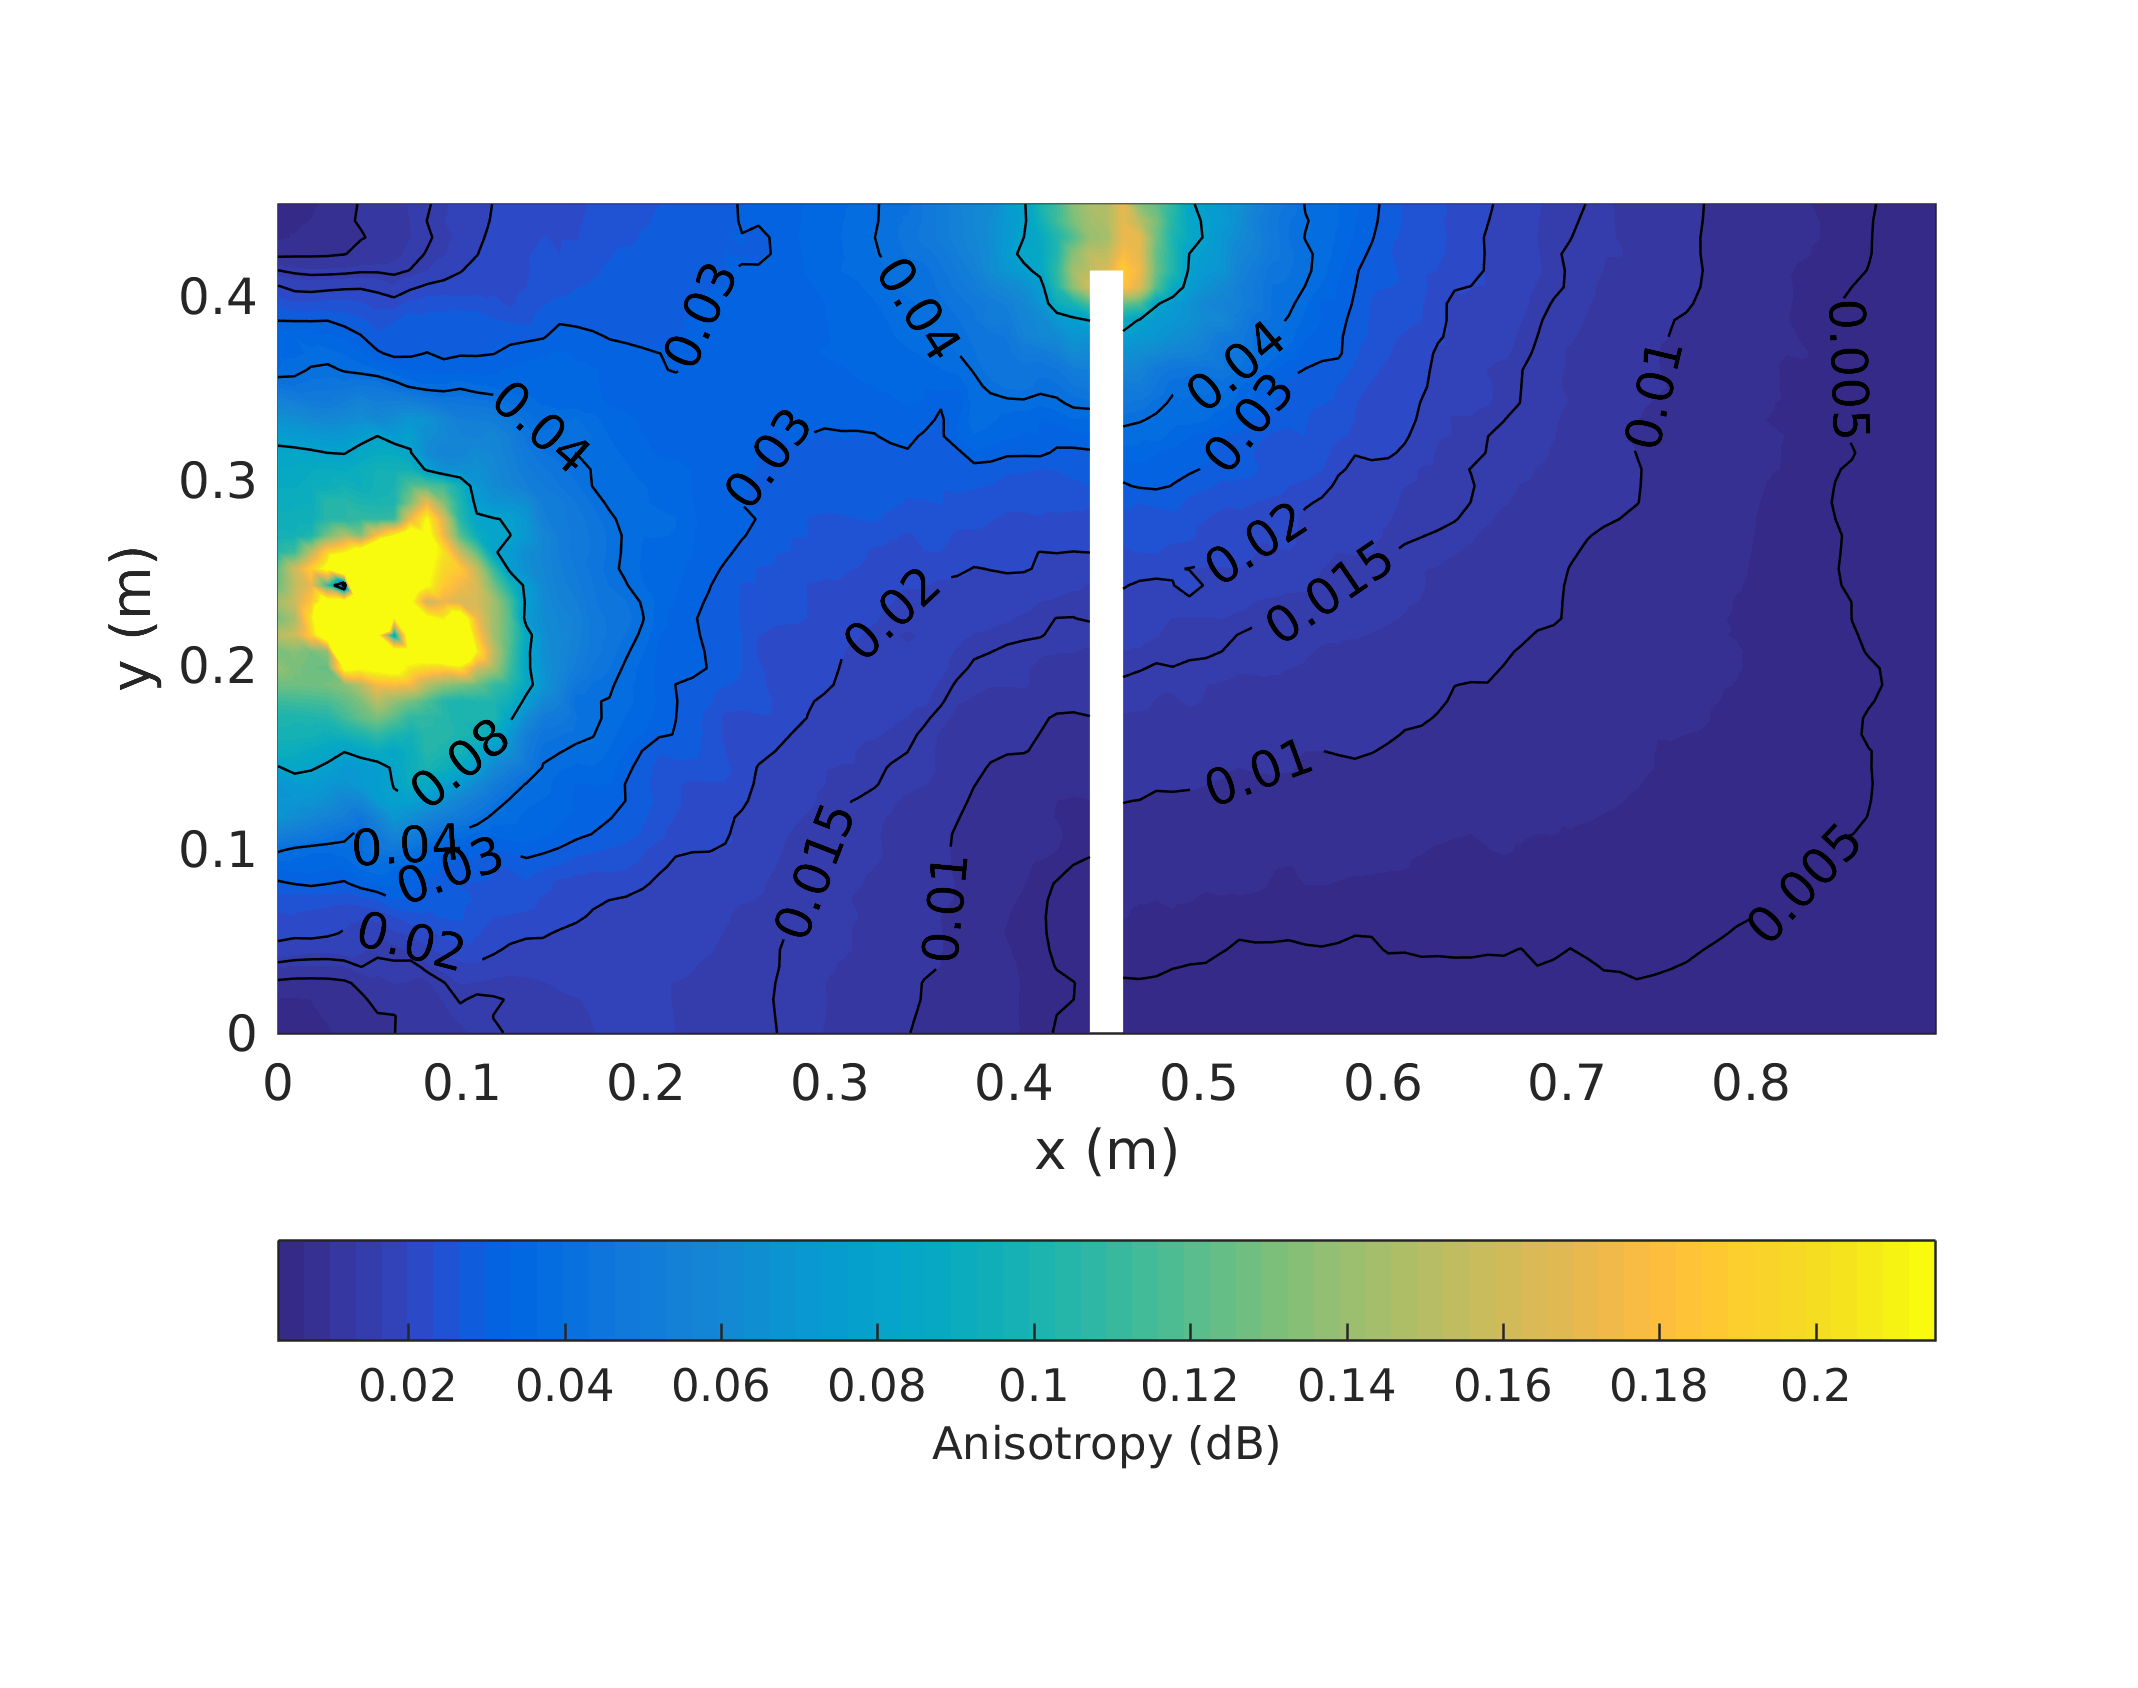
\includegraphics[trim={0 8mm 0 12mm},clip,width=0.52\linewidth]{figures/DDM-EEBC_3D_DU_EnergyDensityAnisotropyMap}\\
{\footnotesize (c)}\\
\vspace{2mm}
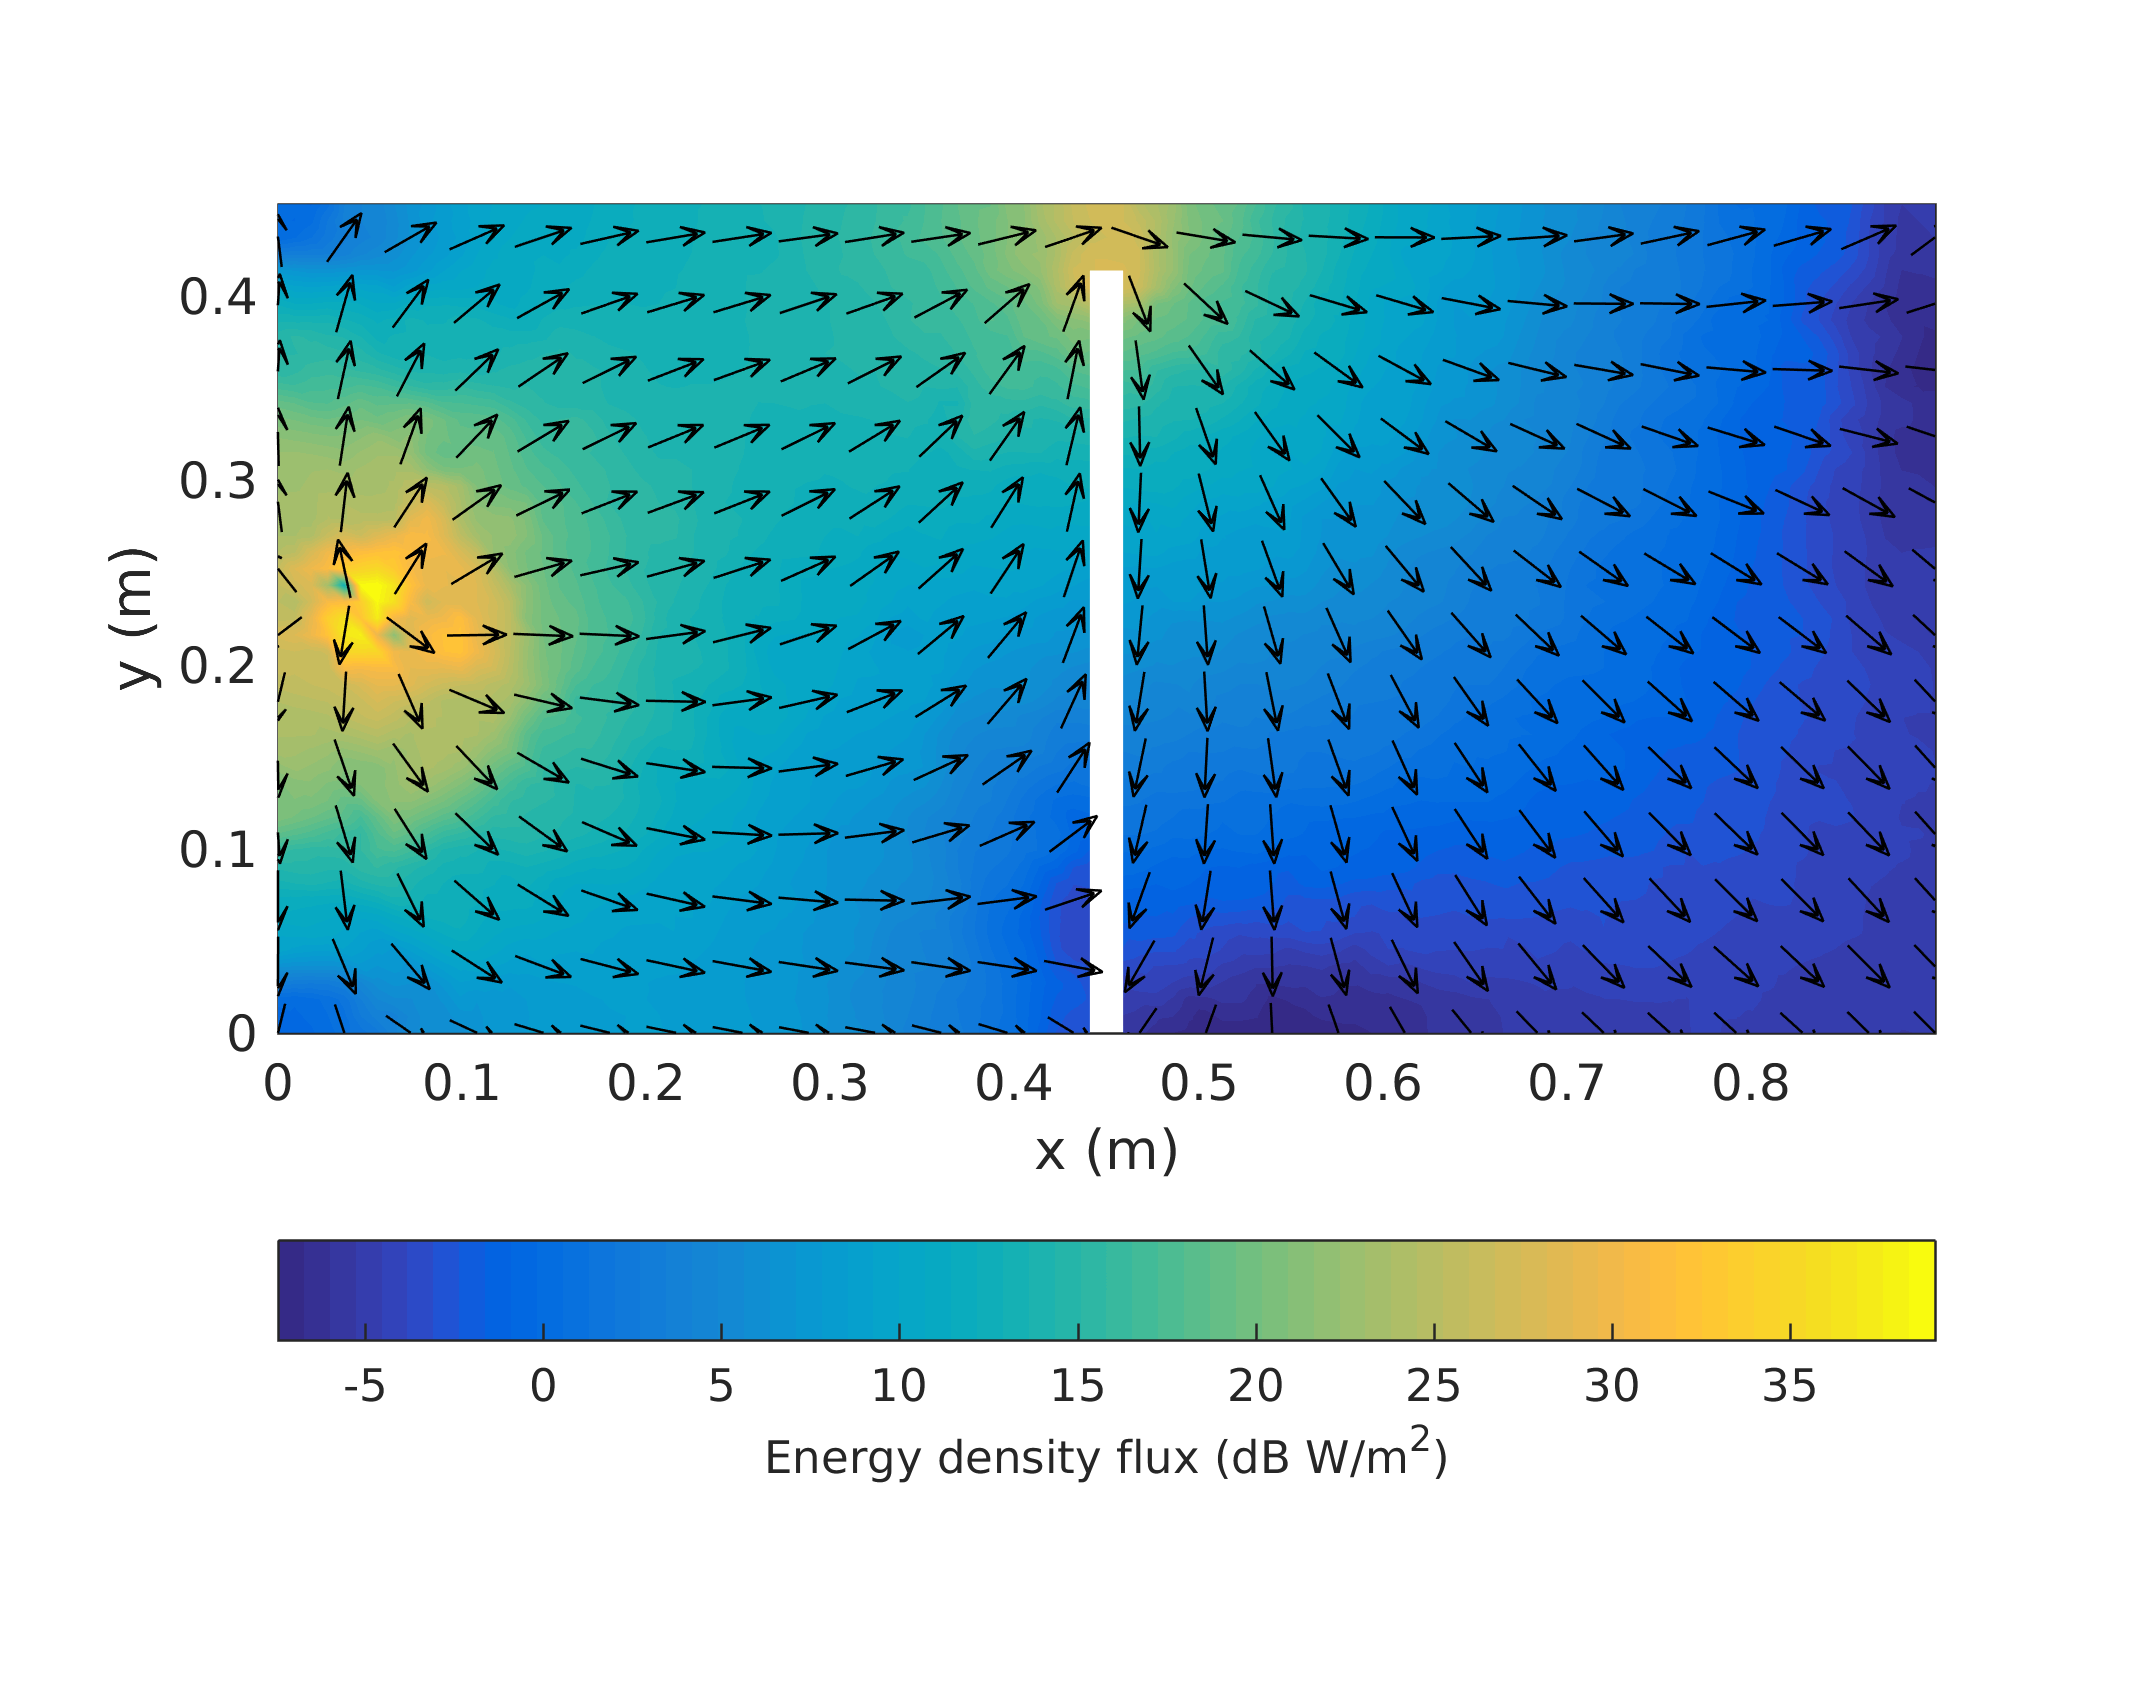
\includegraphics[trim={0 8mm 0 12mm},clip,width=0.52\linewidth]{figures/DDM-EEBC_3D_DU_EnergyDensityFluxMap}\\
{\footnotesize (d)}\\
\vspace{-2mm}
\caption{\label{fg:partemptyddm_maps} Dual domain EEBC 3D EDM maps in the $z$-normal plane at the half height of the cavity for the 
unloaded partitioned cavity: (a) Power density; (b) Energy density relative to the homogeneous PWB model;
(c) Anisotropy; (d) Energy density flux.}
\end{center}
\end{figure}

\subsection[Partitioned cavity with a cylinder]{Partitioned cavity with a cylinder}
\label{sc:res:cylpart}

The derived parameters for the partitioned cavity loaded with the cylinder are given in Table~\ref{tb:derivparamdl} 
and the summary statistics for the average power density in the EDM models are presented in Table~\ref{tb:partcyl}. 
Results are again given for 2D and 3D SDM cases, EEBC and SDM models for the hole, and also for the homogeneous 
PWB model. 

The power density now varies significantly within each sub-cavity and the difference in level between the sub-cavities is
also much greater. Again the 2D and 3D models are in reasonable agreement regarding the basic statistics of the 
average power density. The level difference between the SDM and EEBC models for the hole is now accentuated. 
The COV in the energy density in the source sub-cavity is about 6\,\% for the SDM model and only 2\,\% for the EEBC model.
Note that this difference in COV is mainly due to the difference in the average energy densities between the two
models. The COV in the coupled cavity is much higher at about 20\,\% for both the SDM and EEBC models, which are
closer in absolute level in this sub-cavity.

\begin{table}[H]
\begin{center}
\begin{tabular}{|c|c|c|c|}
\hline
\textbf{Parameter}     &\textbf{Unit} &\textbf{Source sub-cavity} &\textbf{Coupled sub-cavity}\\ 
\hline
\texttt{wallArea}      &m$^2$         &1.0080                     &0.99229             \\
\texttt{partArea}      &m$^2$         &0.18450                    &0.18450             \\
\texttt{holeArea}      &m$^2$         &0.018000                   &0.018000            \\
\texttt{cavityArea}    &m$^2$         &1.2105                     &1.3362              \\
\texttt{cavityVolume}  &m$^3$         &0.090619                   &0.087084            \\
\texttt{wallMFP}       &m             &0.35960                    &0.35104             \\
\texttt{partMFP}       &m             &1.9646                     &1.8880              \\
\texttt{cavityMFP}     &m             &0.29944                    &0.26070             \\
\texttt{wallD}         &m$^2$/s       &3.5935$\times 10^7$        &3.5080$\times 10^7$ \\
\texttt{partD}         &m$^2$/s       &1.9633$\times 10^8$        &1.8867$\times 10^8$ \\
\texttt{cylD}          &m$^2$/s       &-                          &2.4623$\times 10^8$ \\
\texttt{cavityD}       &m$^2$/s       &2.9924$\times 10^7$        &2.6052$\times 10^7$ \\
\texttt{wallACS}       &m$^2$         &0.00068040                 &0.00066980          \\
\texttt{partACS}       &m$^2$         &0.00012454                 &0.00012454          \\
\texttt{cavityACS}     &m$^2$         &0.00080494                 &0.034370            \\
\hline
\end{tabular}
\end{center}
\caption{\label{tb:derivparamdl} Derived parameters for the loaded partitioned cavity.}
\end{table}

\begin{table}[H]
\begin{center}
\begin{tabular}{|l|c|c|c|c|c|}
\hline
\textbf{Power density}               &\textbf{PWB} &\multicolumn{4}{|c|}{\textbf{EDM}} \\ \cline{3-6}
{}                                   &{}           &\textbf{2D SDM} &\textbf{2D DDM} &\textbf{3D SDM} &\textbf{3D DDM} \\
\hline
\multicolumn{6}{|l|}{\textbf{Sub-cavity 1}} \\
\hline
Value at centre (dB\,W\,m$^{-2})$    &23.20        &20.24           &24.25           &20.06           &24.22 \\
Mean (dB\,W\,m$^{-2})$               &23.20        &20.22           &24.24           &20.04           &24.21 \\
Minimum (dB\,W\,m$^{-2})$            &23.20        &18.36           &23.66           &18.18           &20.89 \\
Maximum (dB\,W\,m$^{-2})$            &23.20        &20.70           &24.43           &20.90           &24.51 \\
Standard deviation (dB\,W\,m$^{-2})$ &0            &8.24            &7.78            &7.91            &7.46  \\
Coefficient of variation (\%)        &0            &6.36            &2.26            &6.13            &2.11  \\
\hline
\multicolumn{6}{|l|}{\textbf{Sub-cavity 2}} \\
\hline
Value at centre (dB\,W\,m$^{-2})$    &13.84        &14.27           &13.60           &14.29           &13.63 \\
Mean (dB\,W\,m$^{-2})$               &13.84        &14.93           &14.33           &14.95           &14.28 \\
Minimum (dB\,W\,m$^{-2})$            &13.84        &13.80           &13.09           &13.84           &13.16 \\
Maximum (dB\,W\,m$^{-2})$            &13.84        &18.29           &18.09           &18.24           &17.82 \\
Standard deviation (dB\,W\,m$^{-2})$ &0            &7.94            &7.73            &7.92            &7.30  \\
Coefficient of variation (\%)        &0            &20.0            &21.9            &19.8            &20.0  \\
\hline
\end{tabular}
\end{center}
\caption{\label{tb:partcyl} Statistics of the reverberant power density in the partitioned cavity with the cylinder.}
\end{table}

The variation of the power density in the $z$-direction for the SDM and EEBC model are shown in 
Figure~\ref{fg:partcylsdm_profs}(a) and Figure~\ref{fg:partcylddm_profs}(a) at $y=L_y/2$ and various 
values of $x$. In this case the quadratic anzatz used in the Kantorovich reduction
is seen to be quite accurate away from the source and the 2D model provides very good results. Note, however that
the vertical profile near the aperture ($x=0.44$\,m) for the EEBC is somewhat erratic, perhaps indicating 
some numerical issue. It must always be remembered that the EDM is not expected to valid very close to an aperture,
where the field cannot be highly diffuse. The variation of the power density in the $x$-direction for $z=L_z/2$ 
and a number of $y$ positions is shown in Figure~\ref{fg:partcylsdm_profs}(b) and 
Figure~\ref{fg:partcylddm_profs}(b) for the SDM and EEBC. We again see that the SDM predicts less level difference
between the two cavities than the EEBC and PWB models, which give comparable levels. The SDM result for the loaded
cases is notably less symmetrically placed between the PWB levels than was the case for the unloaded cases. 
The EEBC model predicts a slightly higher power density in the source cavity and its average level is in reasonable
agreement with the PWB model in the coupled cavity. The range of the power density in the coupled sub-cavity is
about 2\,dB for both the SDM and EEBC models with a similar profile. The PDF for the average power density in 
the sub-cavities are shown in Figure~\ref{fg:partcylsdm_profs}(c) and Figure~\ref{fg:partcylddm_profs}(c).

Figure~\ref{fg:partcylsdm_maps} and Figure~\ref{fg:partcylddm_maps} shows maps of various quantities in 
the $z=L_z/2$ plane for the SDM and EEBC model respectively. The power densities are shown in 
Figure~\ref{fg:partcylsdm_maps}(a) and Figure~\ref{fg:partcylddm_maps}(a) as hybrid heat and contour maps; 
the power density again falls off along the source sub-cavity towards the aperture and then in the coupled
sub-cavity increase away from the hole. The uniformities in the SDM and EEBC models are shown in 
Figure~\ref{fg:partcylsdm_maps}(b) and Figure~\ref{fg:partcylddm_maps}(b). In both cases the EDM again
predicts lower values than the PWB model in the source cavity and high values in the coupled cavity, as was
the case for the unloaded partition cavity. The anisotropies are shown in Figure~\ref{fg:partcylsdm_maps}(c) and
Figure~\ref{fg:partcylddm_maps}(c) and are fairly similar for the two aperture models. The anisotropy varies up to
about 1.5\,dB in the cavity and notably remains above 1\,dB in the volume of the coupled sub-cavity between the 
hole and the cylinder. The energy density fluxes shown in Figure~\ref{fg:partcylsdm_maps}(c) and 
Figure~\ref{fg:partcylddm_maps}(c) are fairly similar in structure with some difference in magnitude due to the 
energy density division between the sub-cavities.

\begin{figure}[hp]
\begin{center}
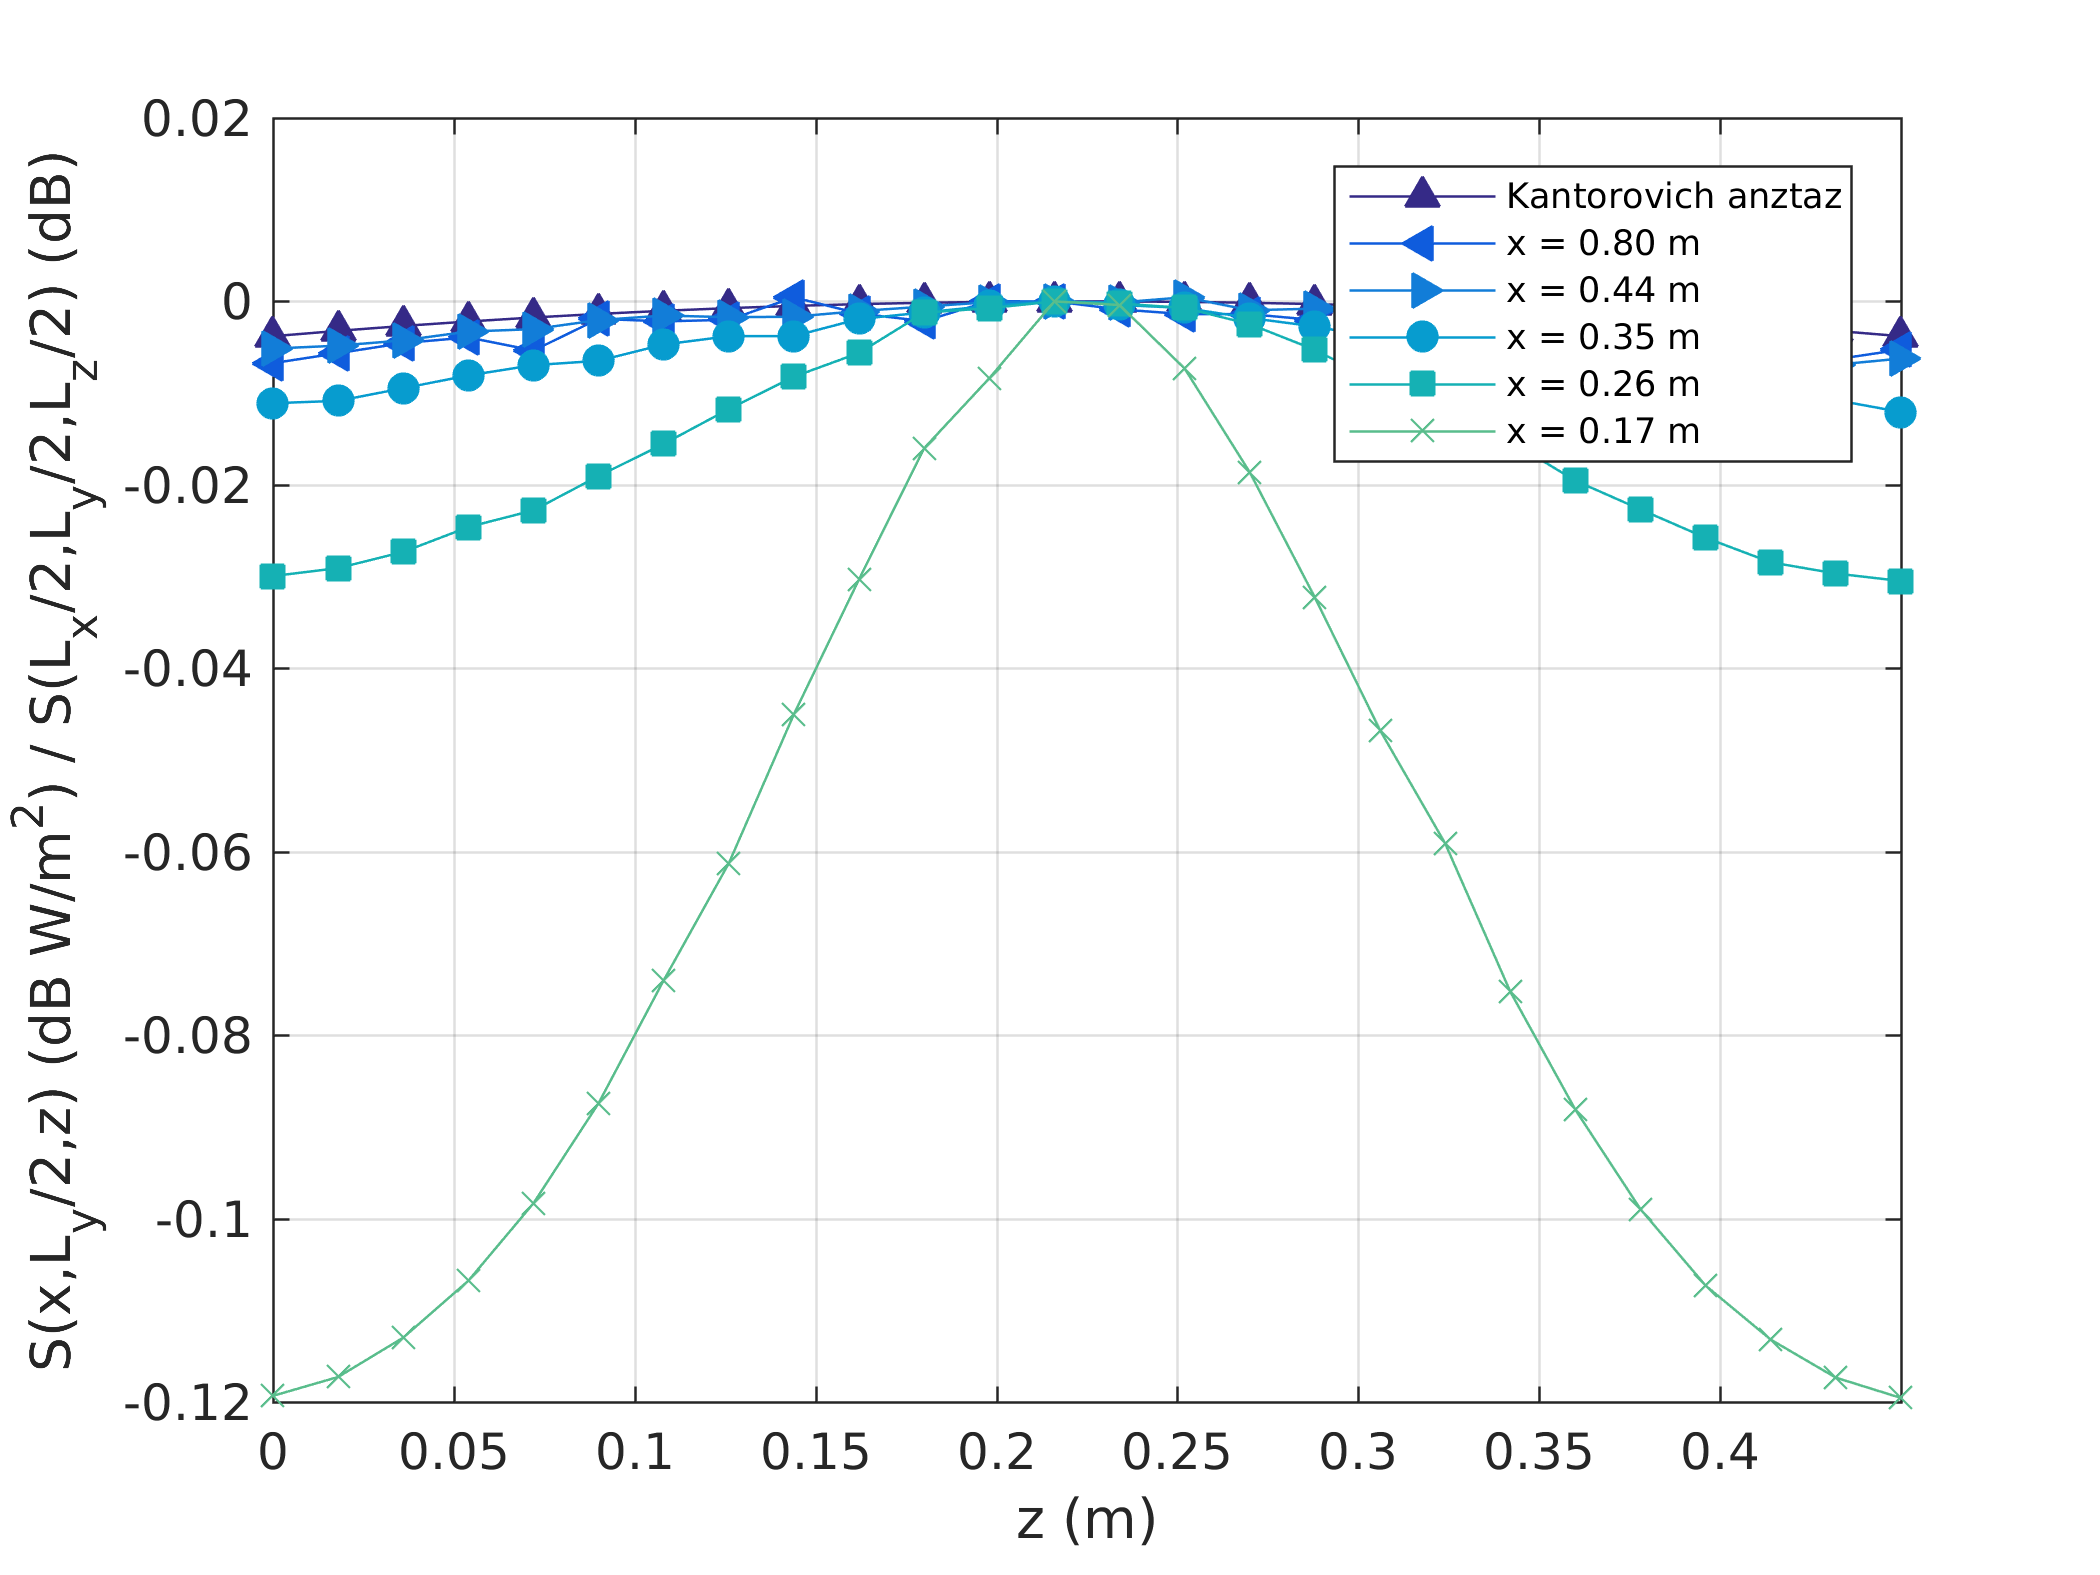
\includegraphics[width=0.6\linewidth]{figures/SDM_3D_DL_PowerDensityProfileZ}\\
{\footnotesize (a)}\\
\vspace{2mm}
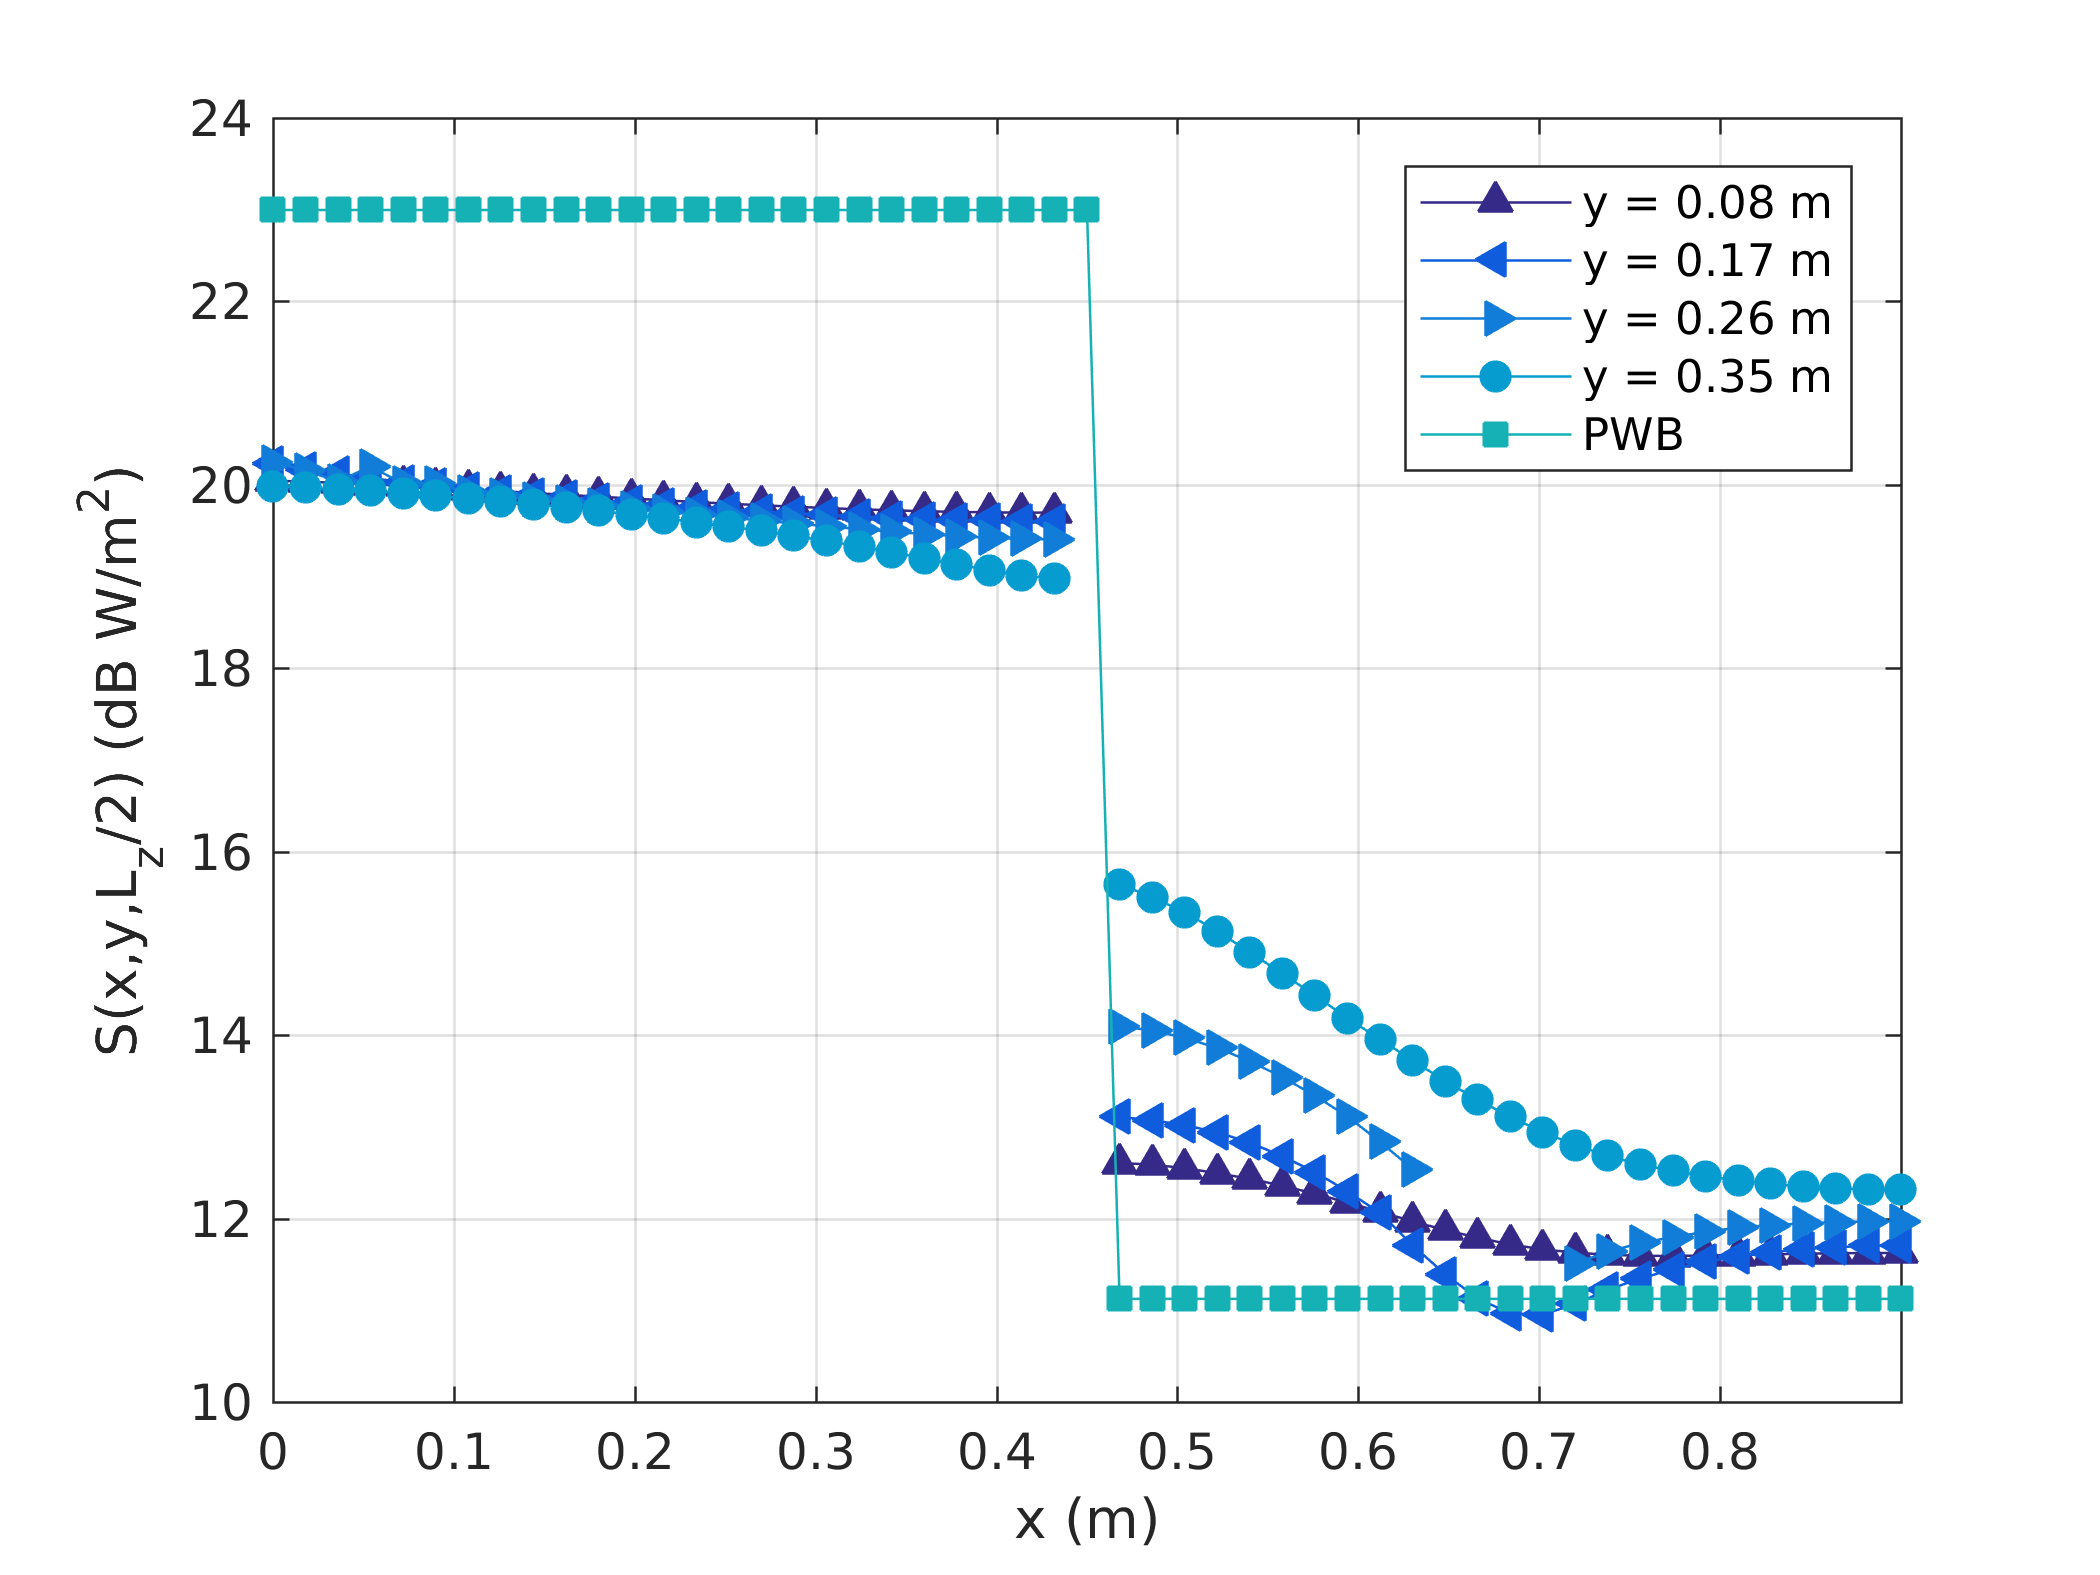
\includegraphics[width=0.6\linewidth]{figures/SDM_3D_DL_PowerDensityProfileX}\\
{\footnotesize (b)}\\
\vspace{2mm}
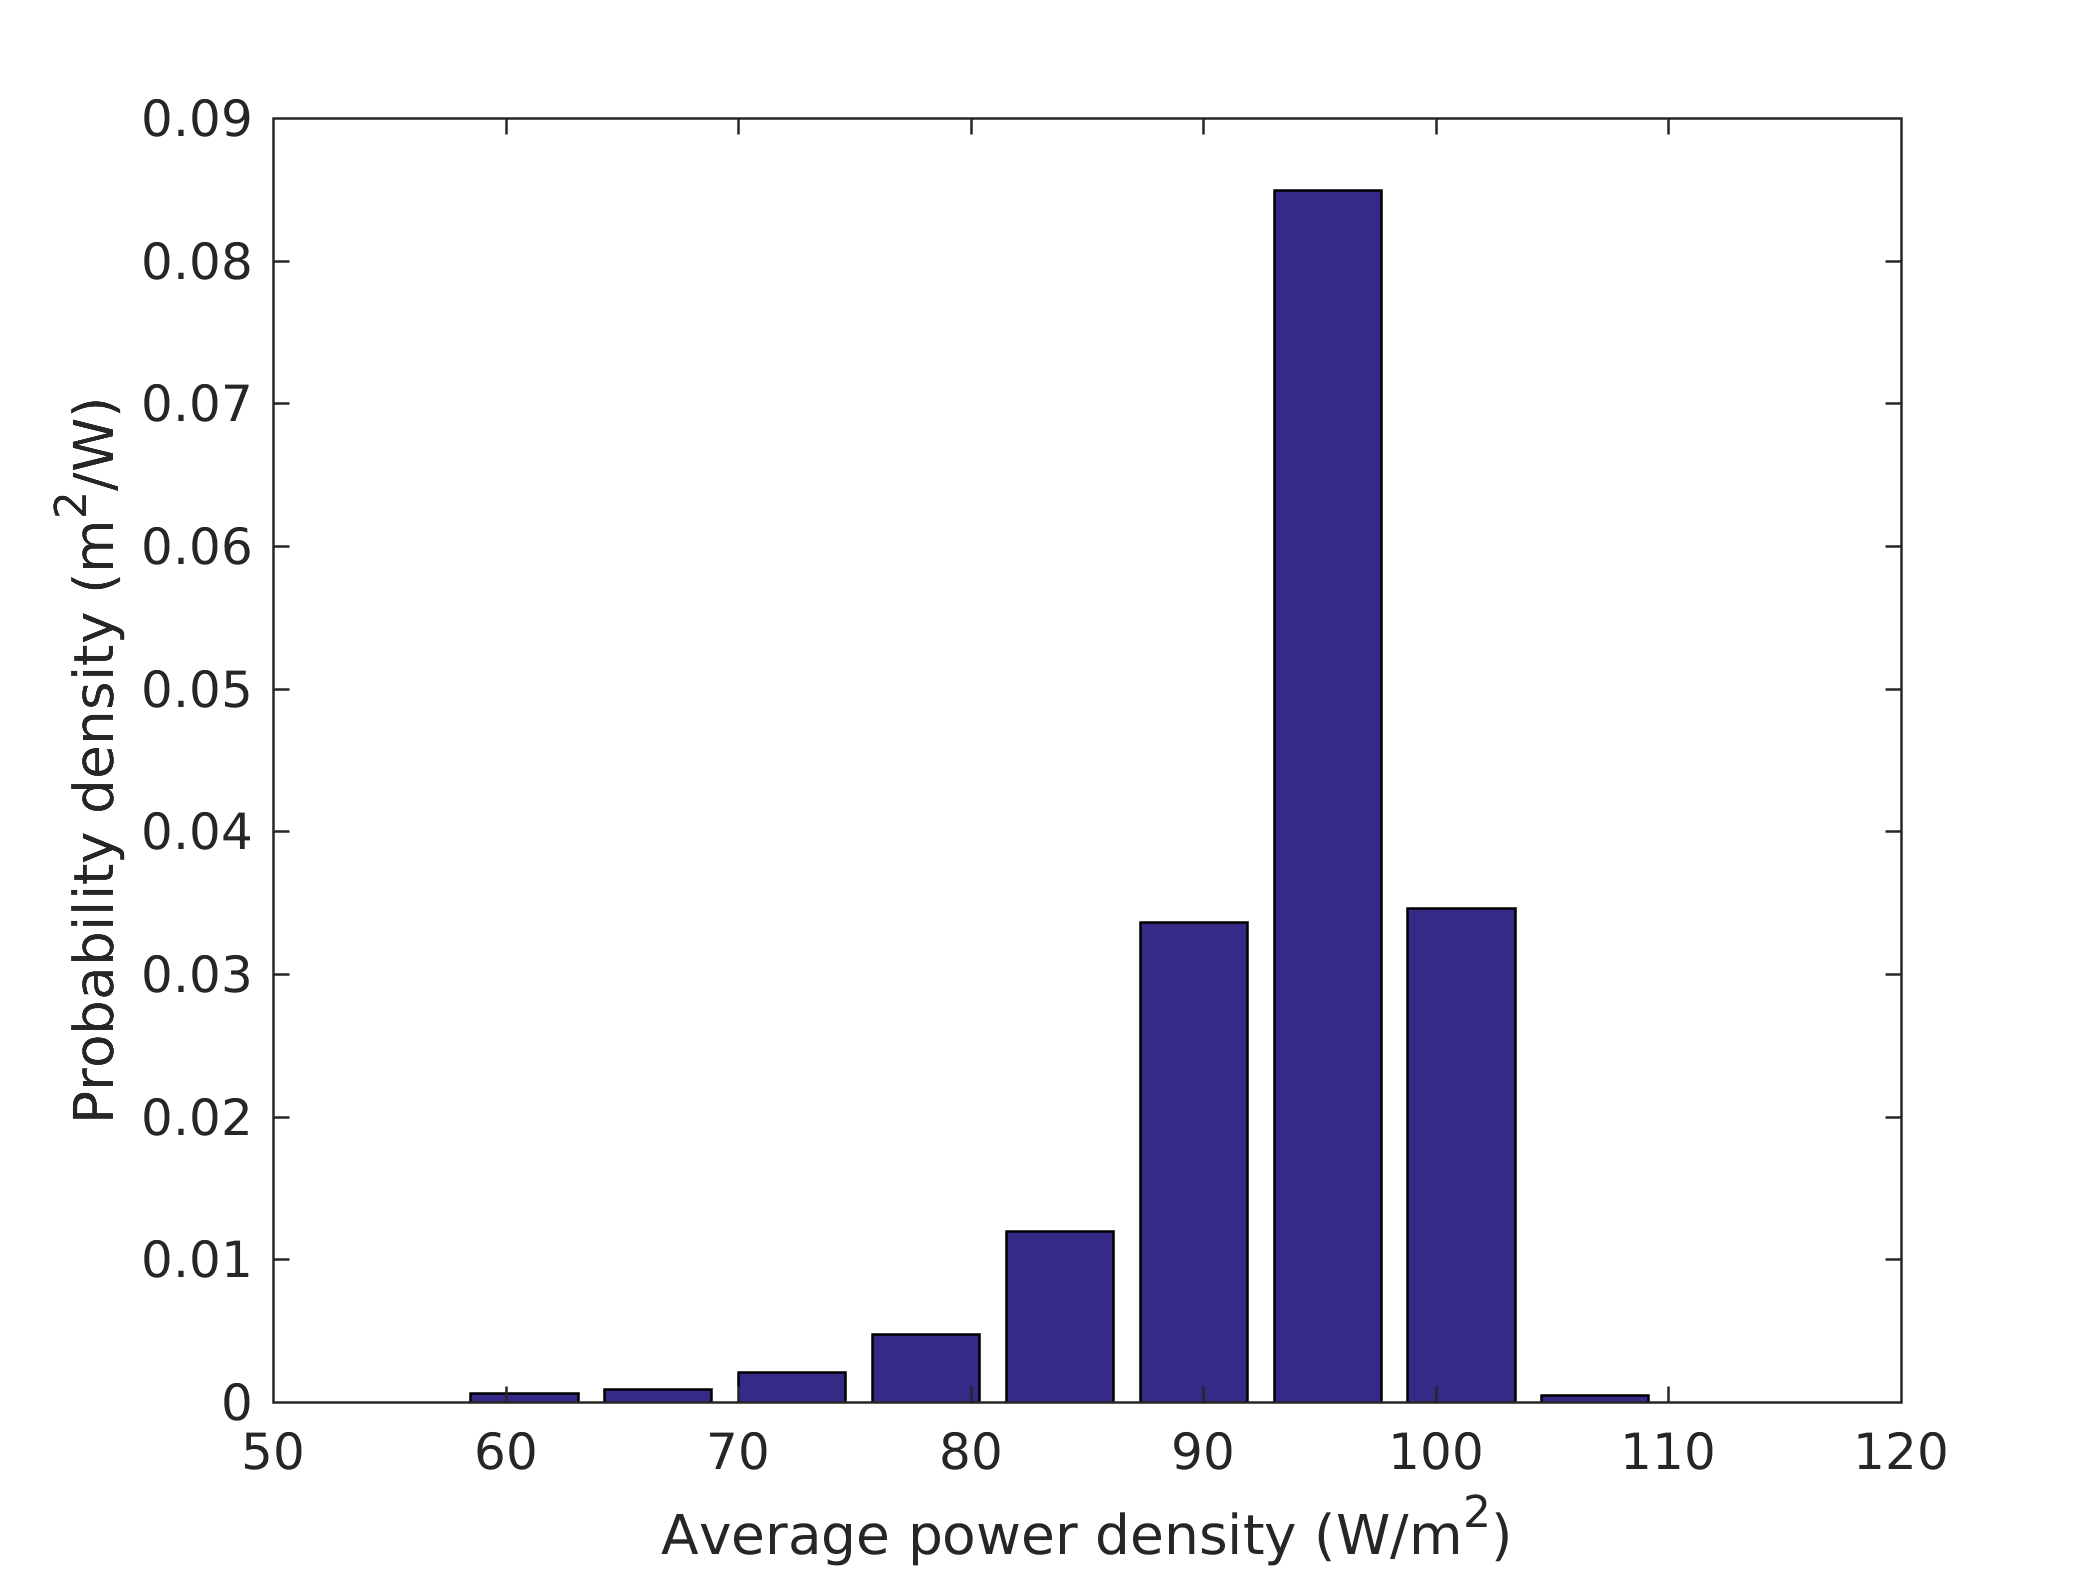
\includegraphics[width=0.45\linewidth]{figures/SDM_3D_DL_PowerDensityPDF1}
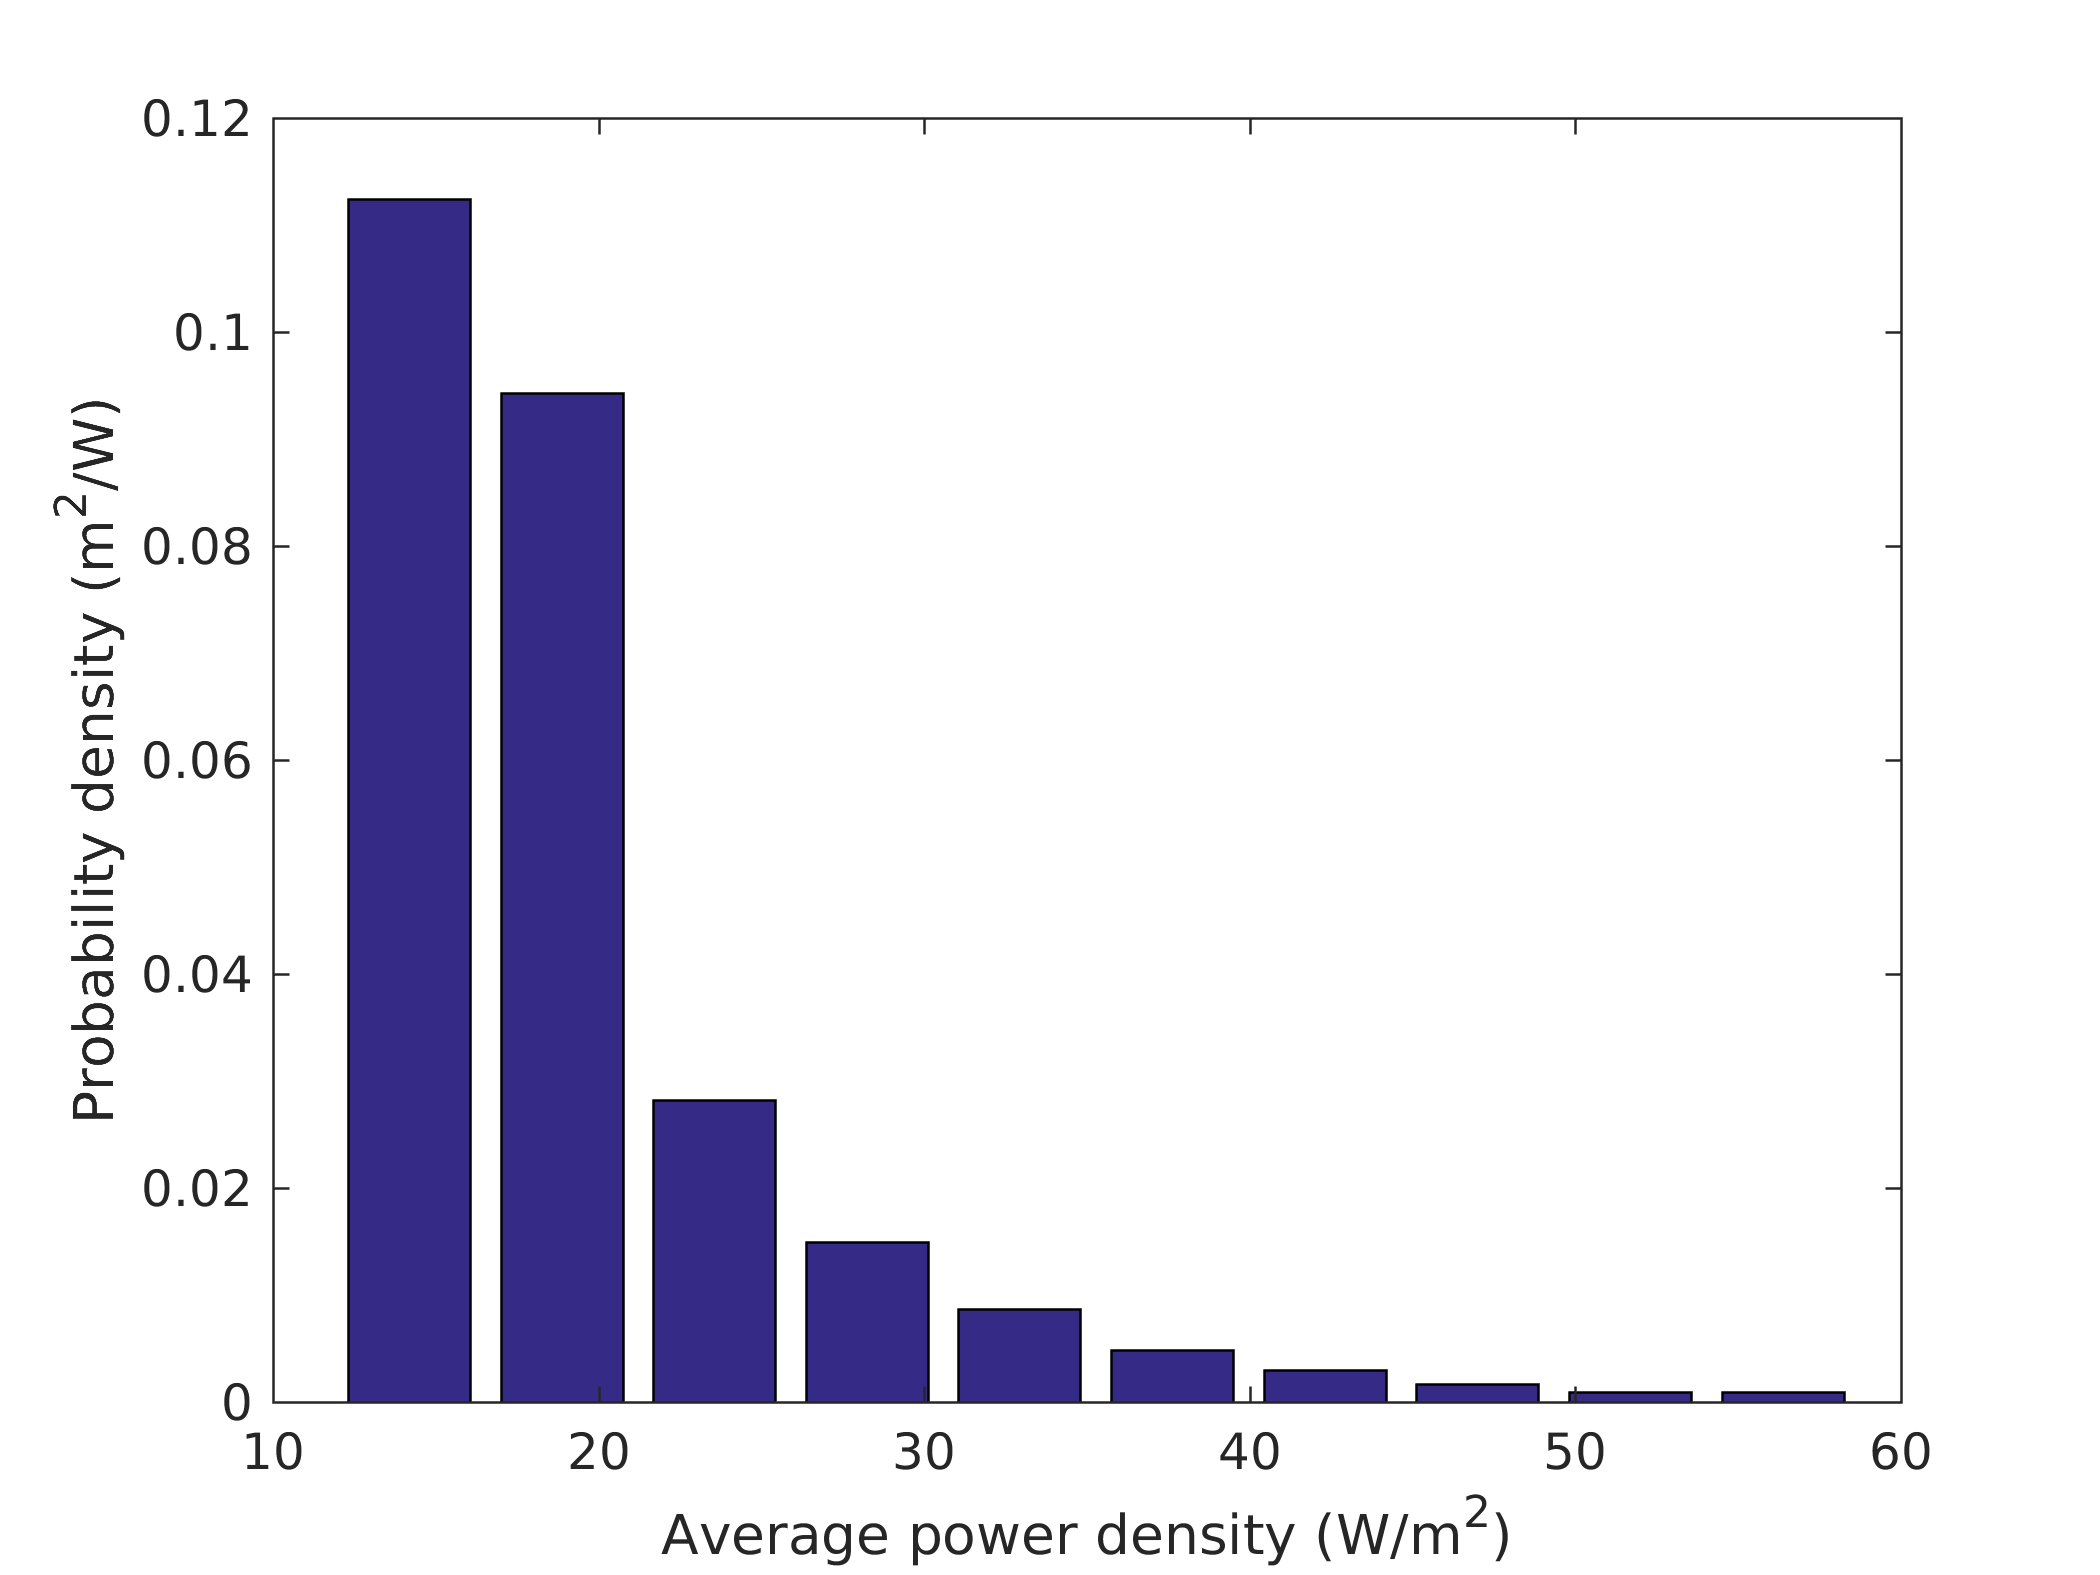
\includegraphics[width=0.45\linewidth]{figures/SDM_3D_DL_PowerDensityPDF2}
\\
{\footnotesize (c)}\\
\vspace{-2mm}
\caption{\label{fg:partcylsdm_profs} Single domain EDM of the loaded partitioned cavity: (a) Normalised vertical profile of the power density; 
(b) Power density profile in the $x$-direction along the cavity centre; (c) PDF of the power density in the source cavity (left) and coupled cavity (right).}
\end{center}
\end{figure}

\begin{figure}[hp]
\begin{center}
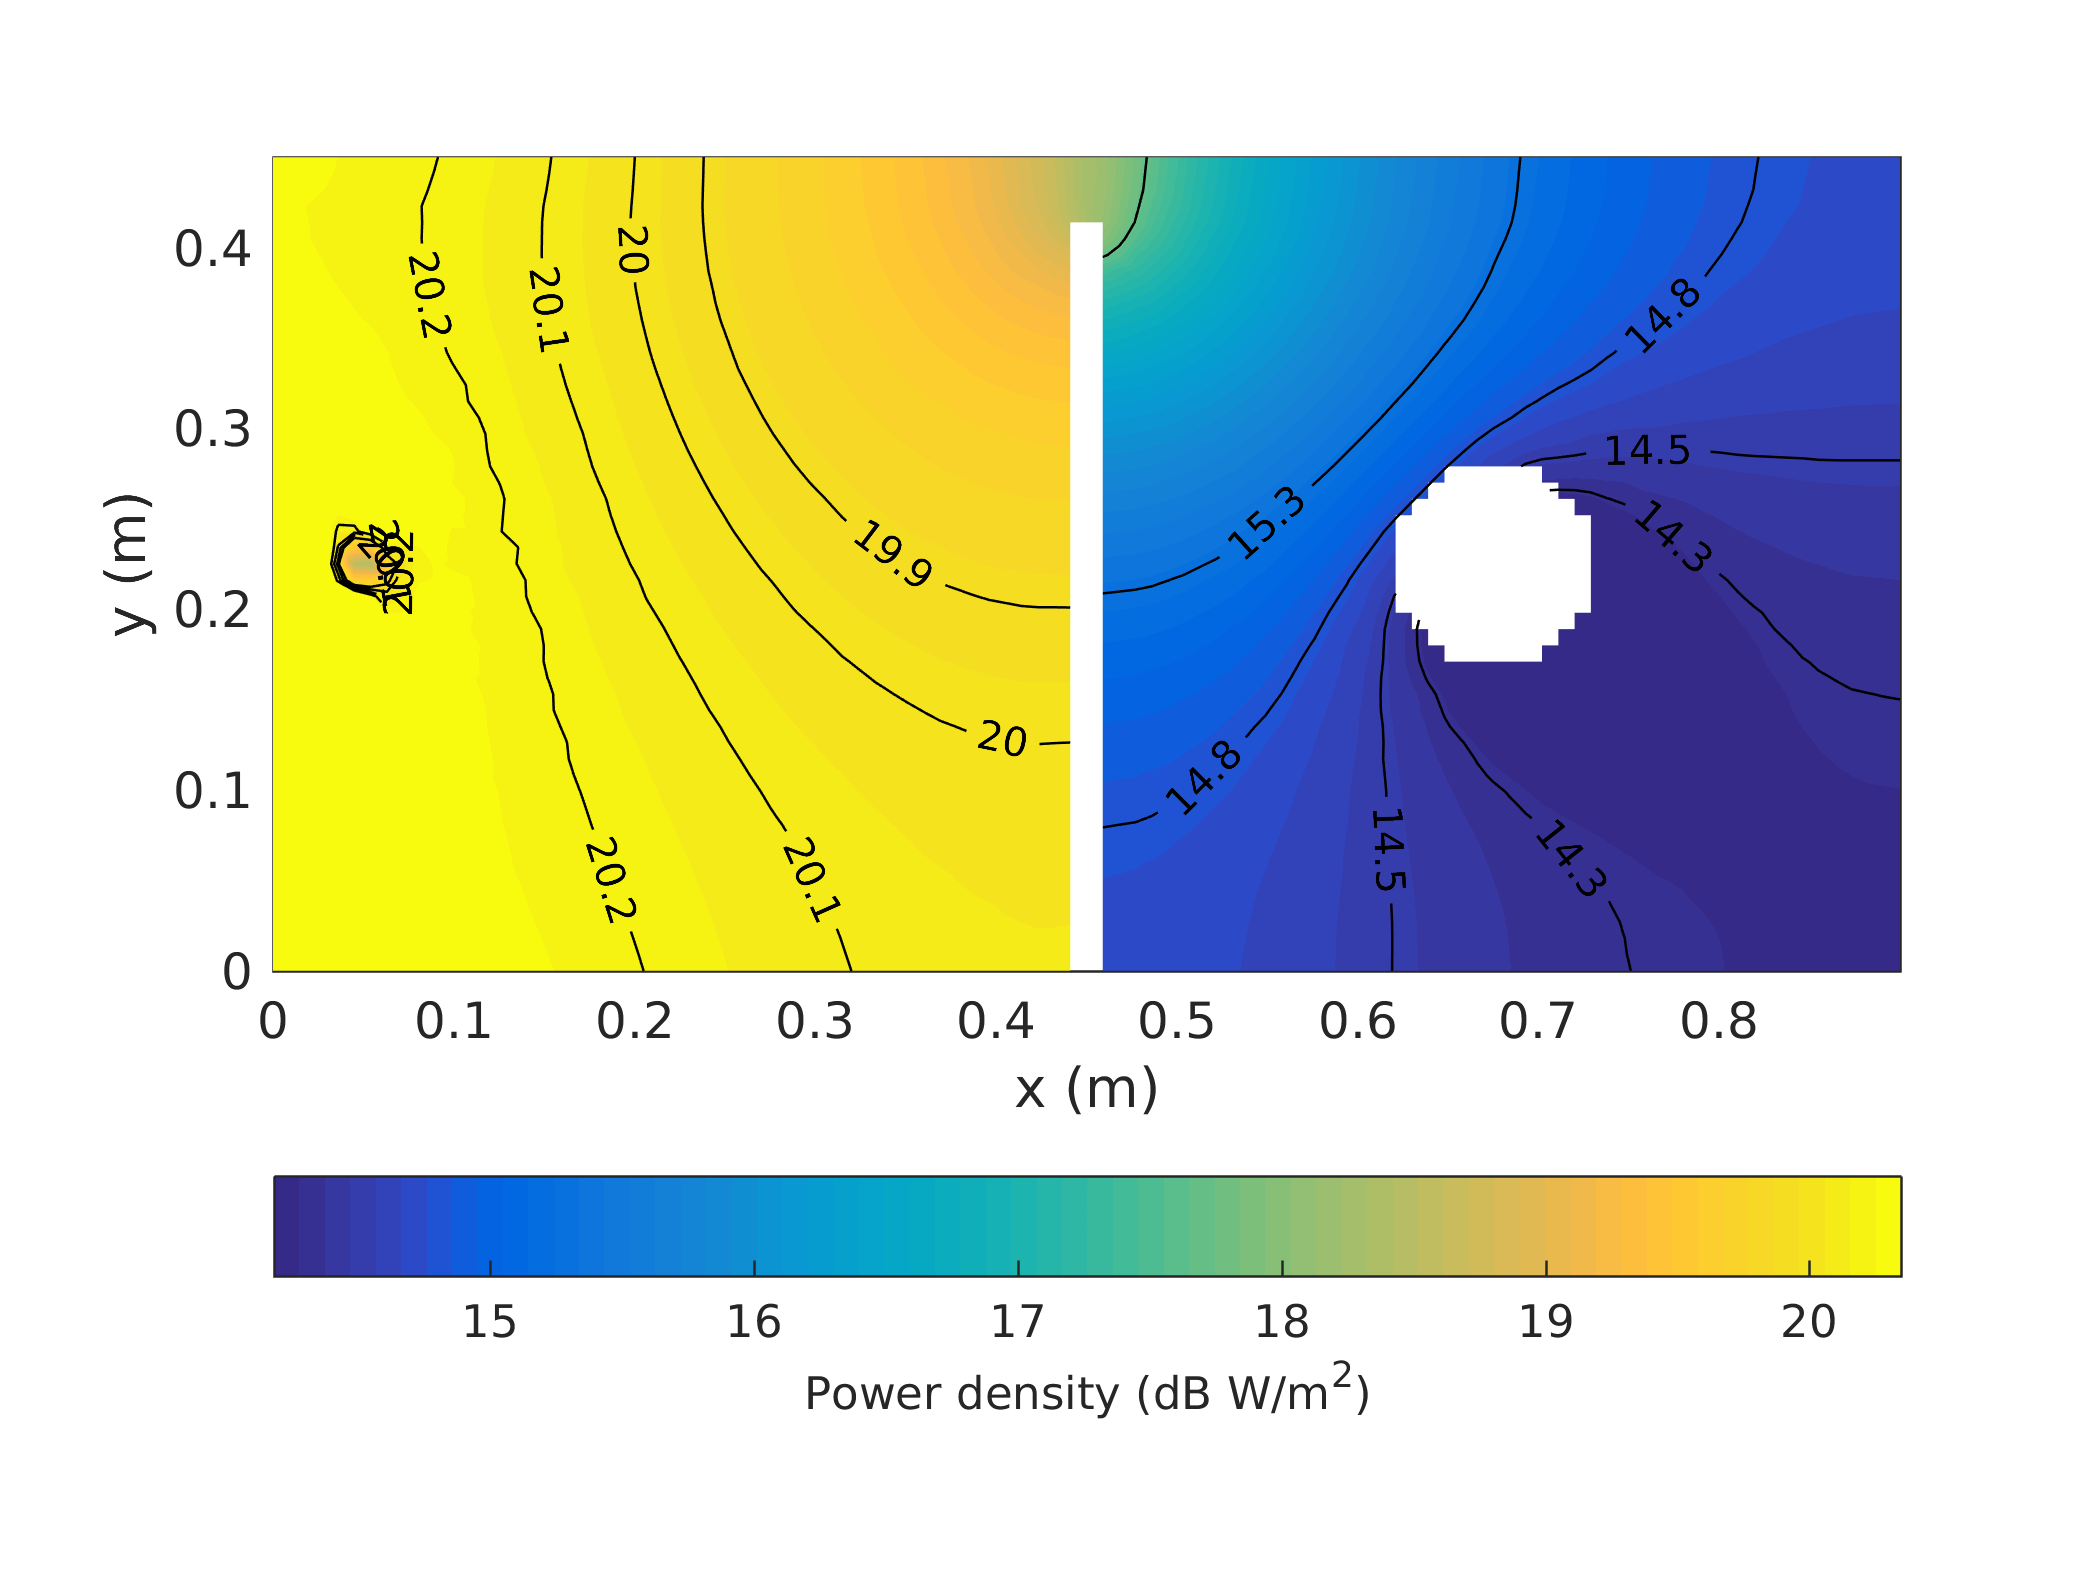
\includegraphics[trim={0 8mm 0 12mm},clip,width=0.52\linewidth]{figures/SDM_3D_DL_PowerDensityMap}\\
{\footnotesize (a)}\\
\vspace{2mm}
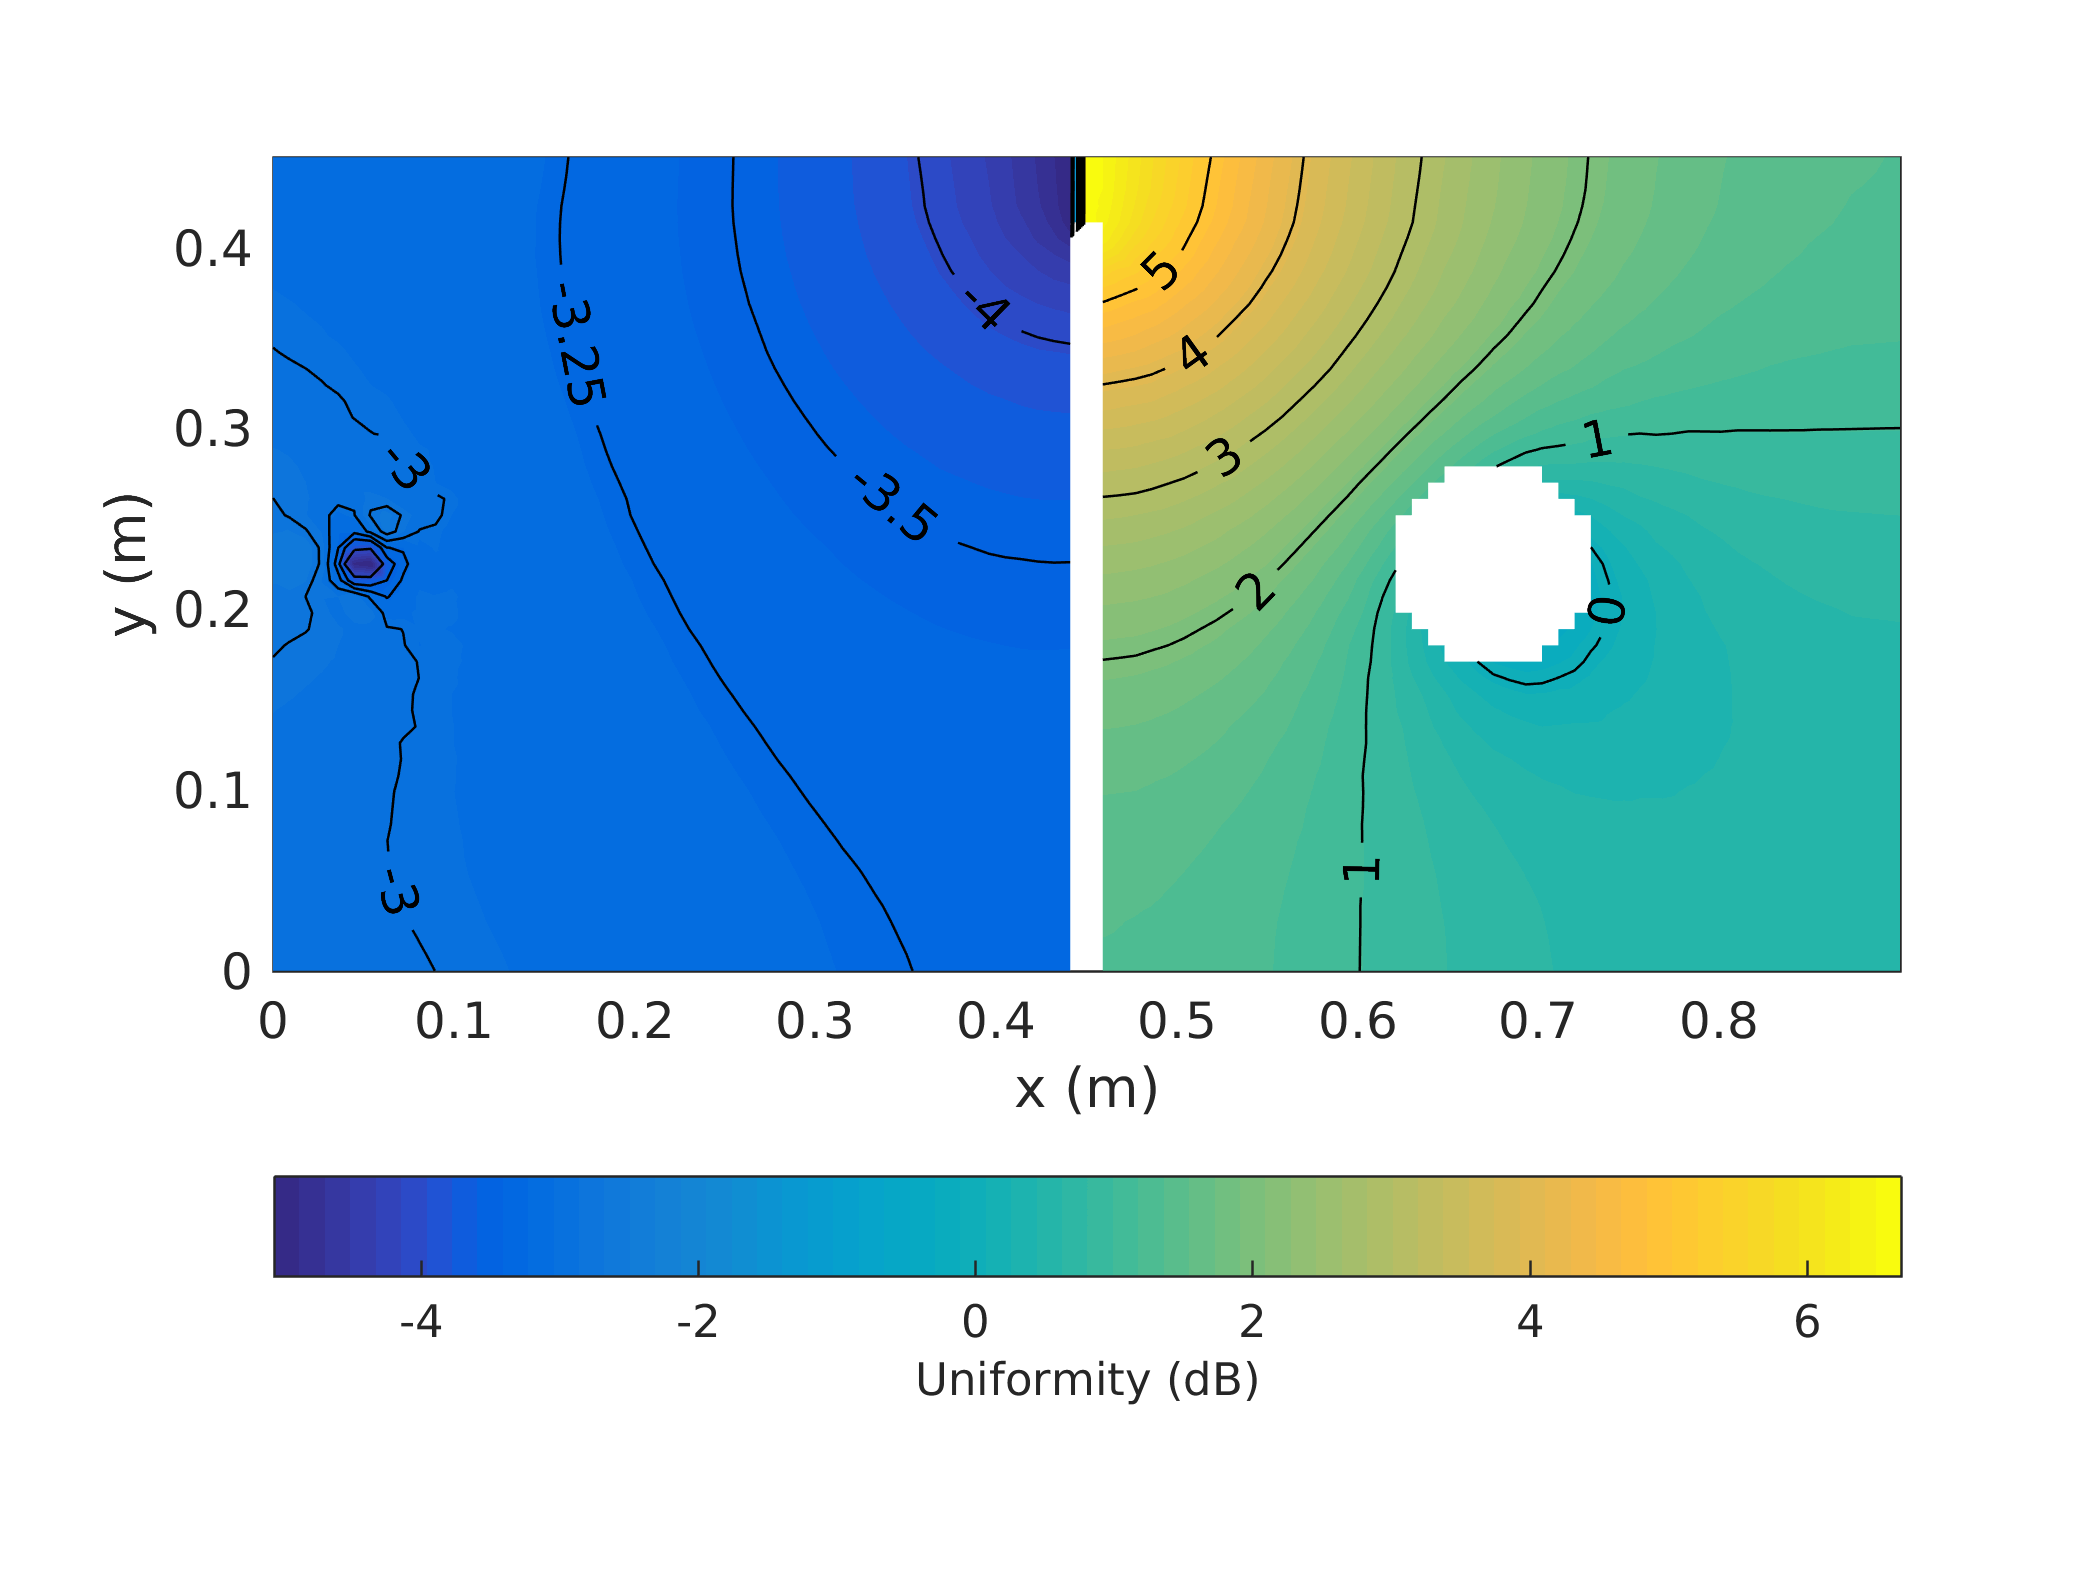
\includegraphics[trim={0 8mm 0 12mm},clip,width=0.52\linewidth]{figures/SDM_3D_DL_EnergyDensityUniformityMap}\\
{\footnotesize (b)}\\
\vspace{2mm}
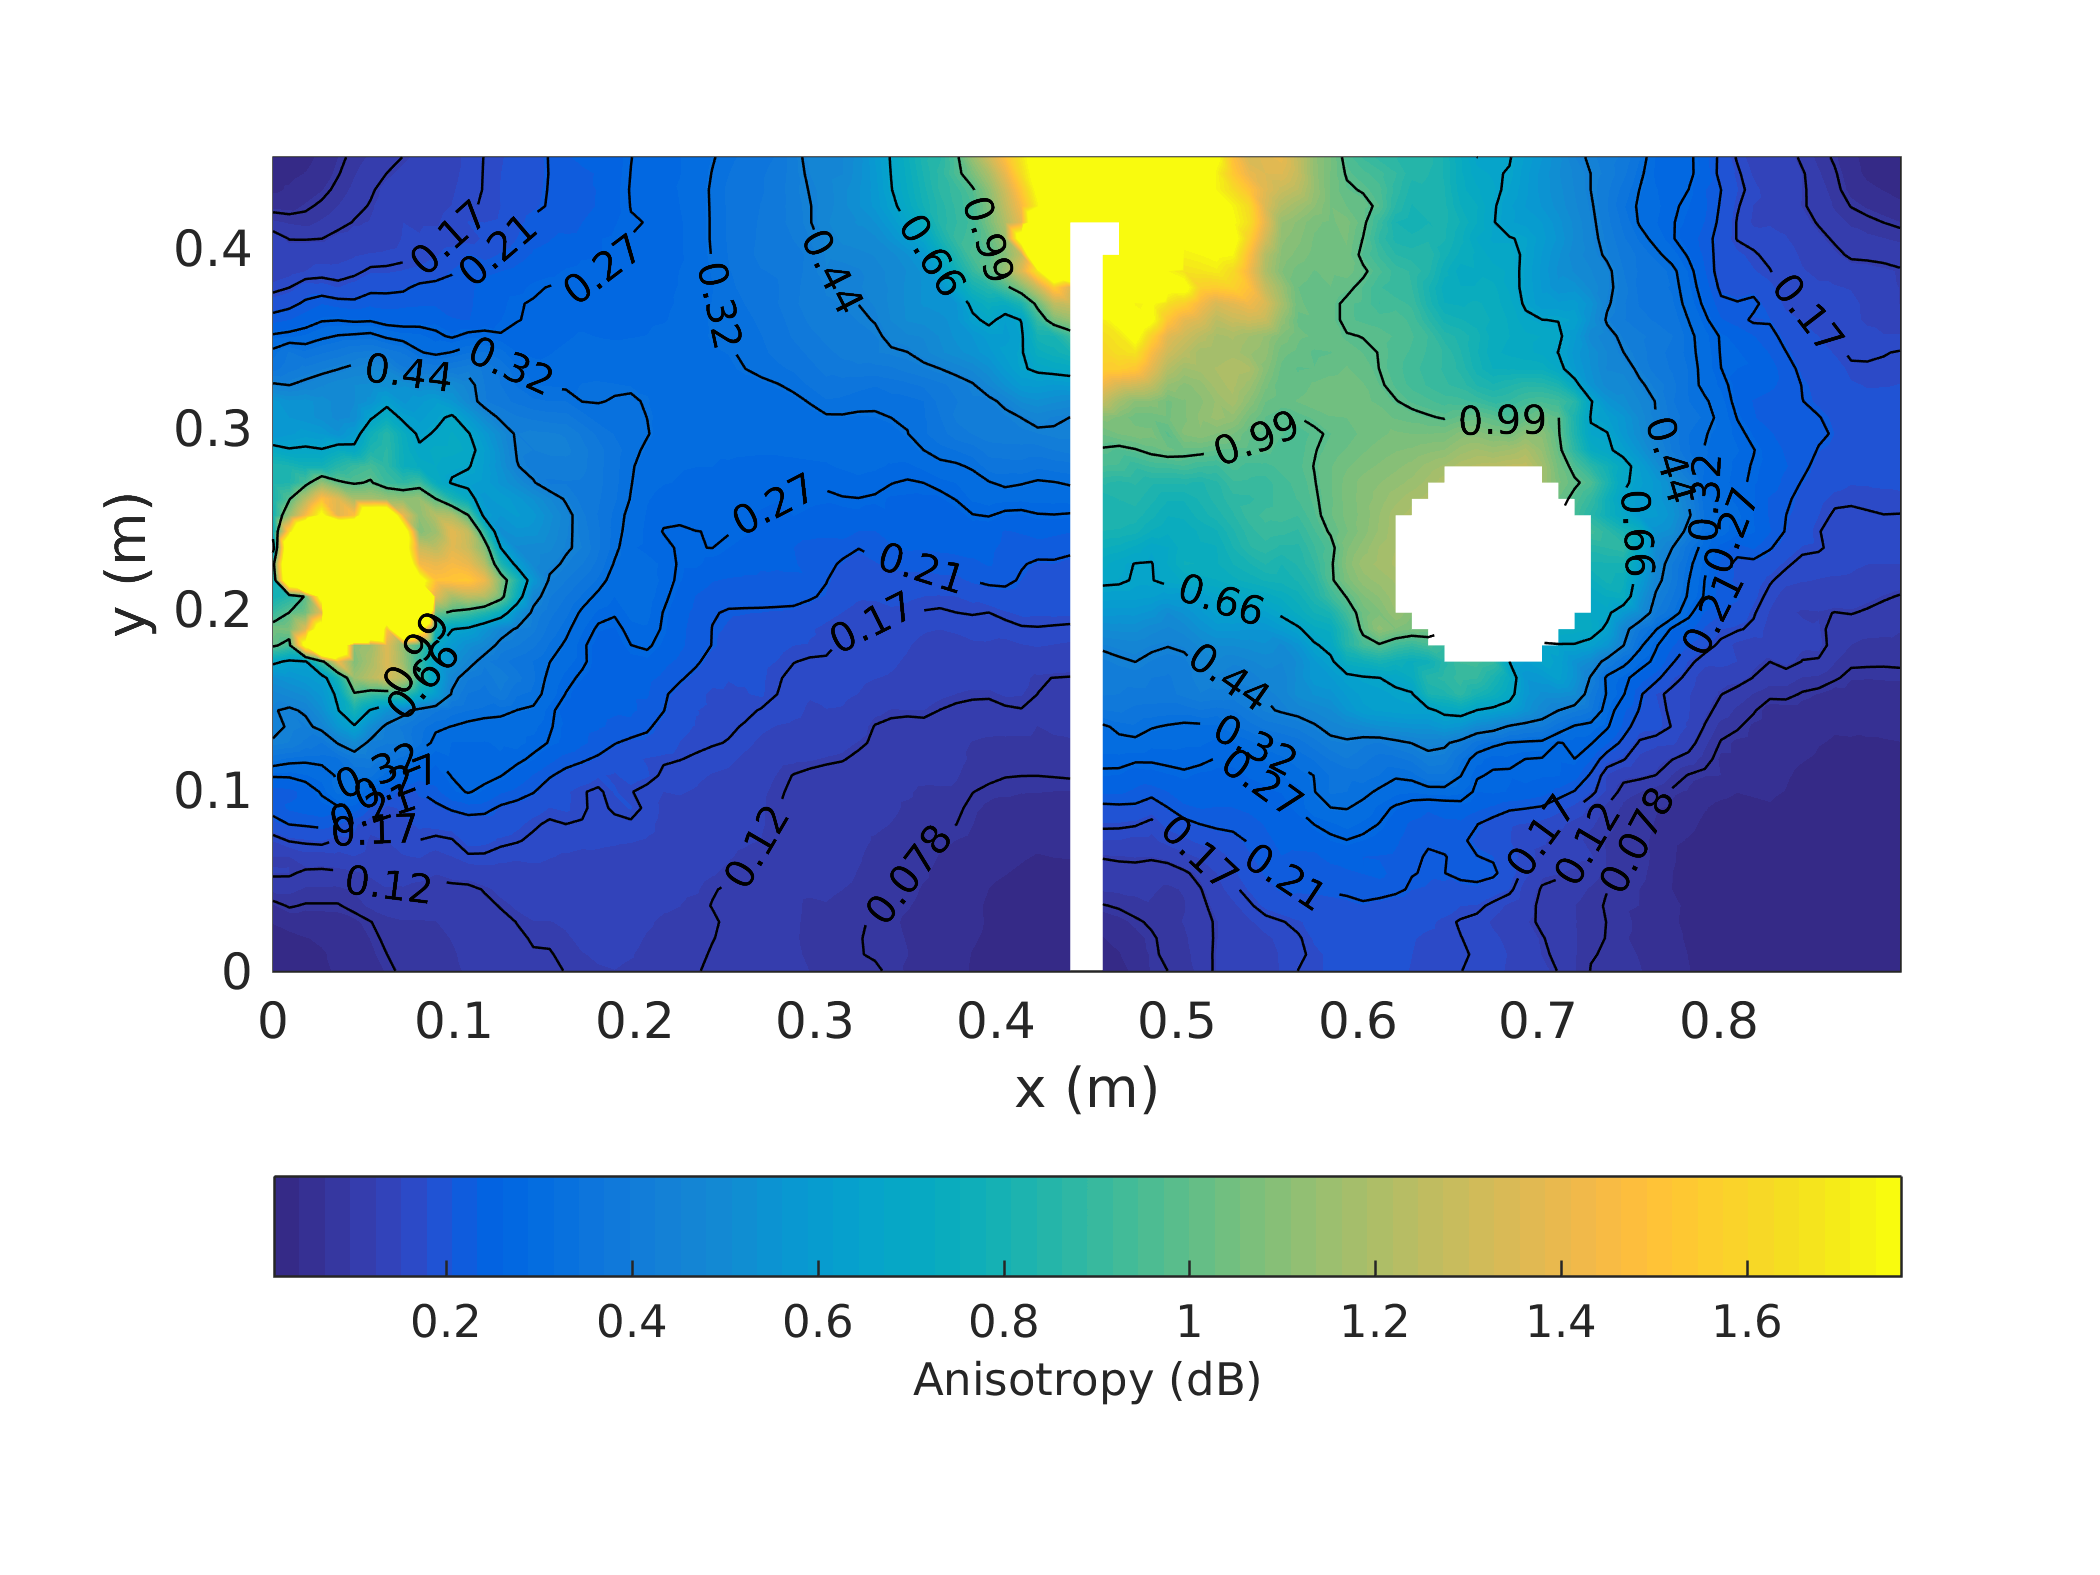
\includegraphics[trim={0 8mm 0 12mm},clip,width=0.52\linewidth]{figures/SDM_3D_DL_EnergyDensityAnisotropyMap}\\
{\footnotesize (c)}\\
\vspace{2mm}
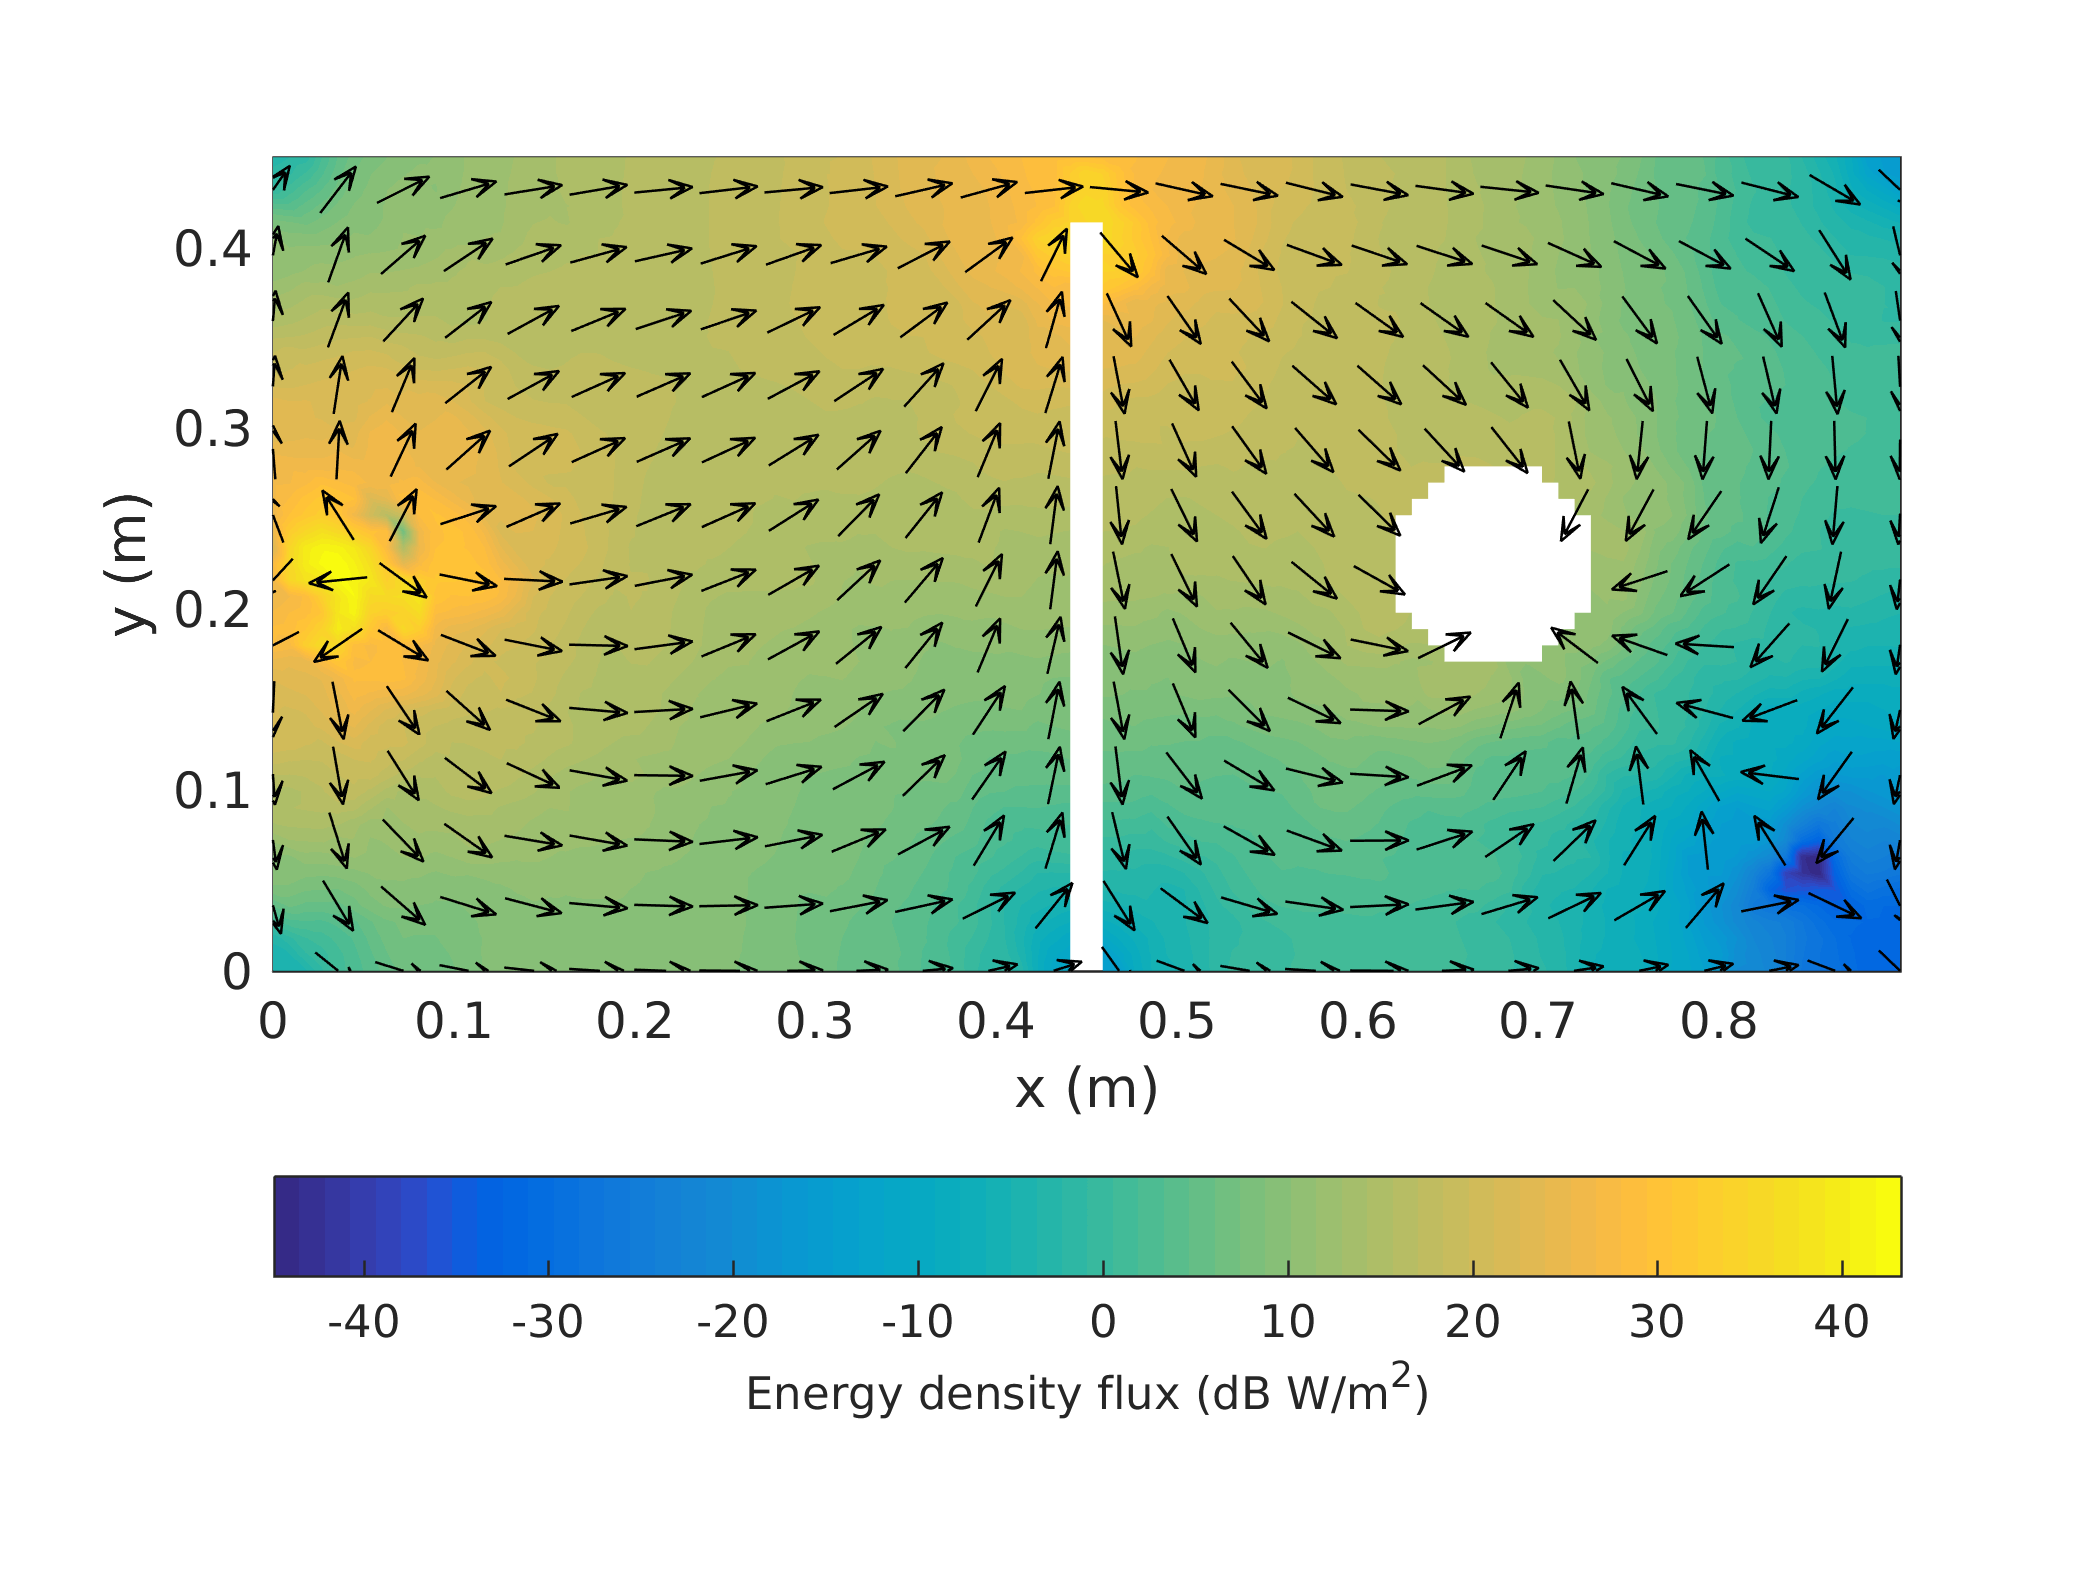
\includegraphics[trim={0 8mm 0 12mm},clip,width=0.52\linewidth]{figures/SDM_3D_DL_EnergyDensityFluxMap}\\
{\footnotesize (d)}\\
\vspace{-2mm}
\caption{\label{fg:partcylsdm_maps} Single domain 3D EDM maps in the $z$-normal plane at the half height of the cavity for the 
loaded partitioned cavity: (a) Power density; (b) Energy density relative to the homogeneous PWB model;
(c) Anisotropy; (d) Energy density flux.}
\end{center}
\end{figure}

\begin{figure}[hp]
\begin{center}
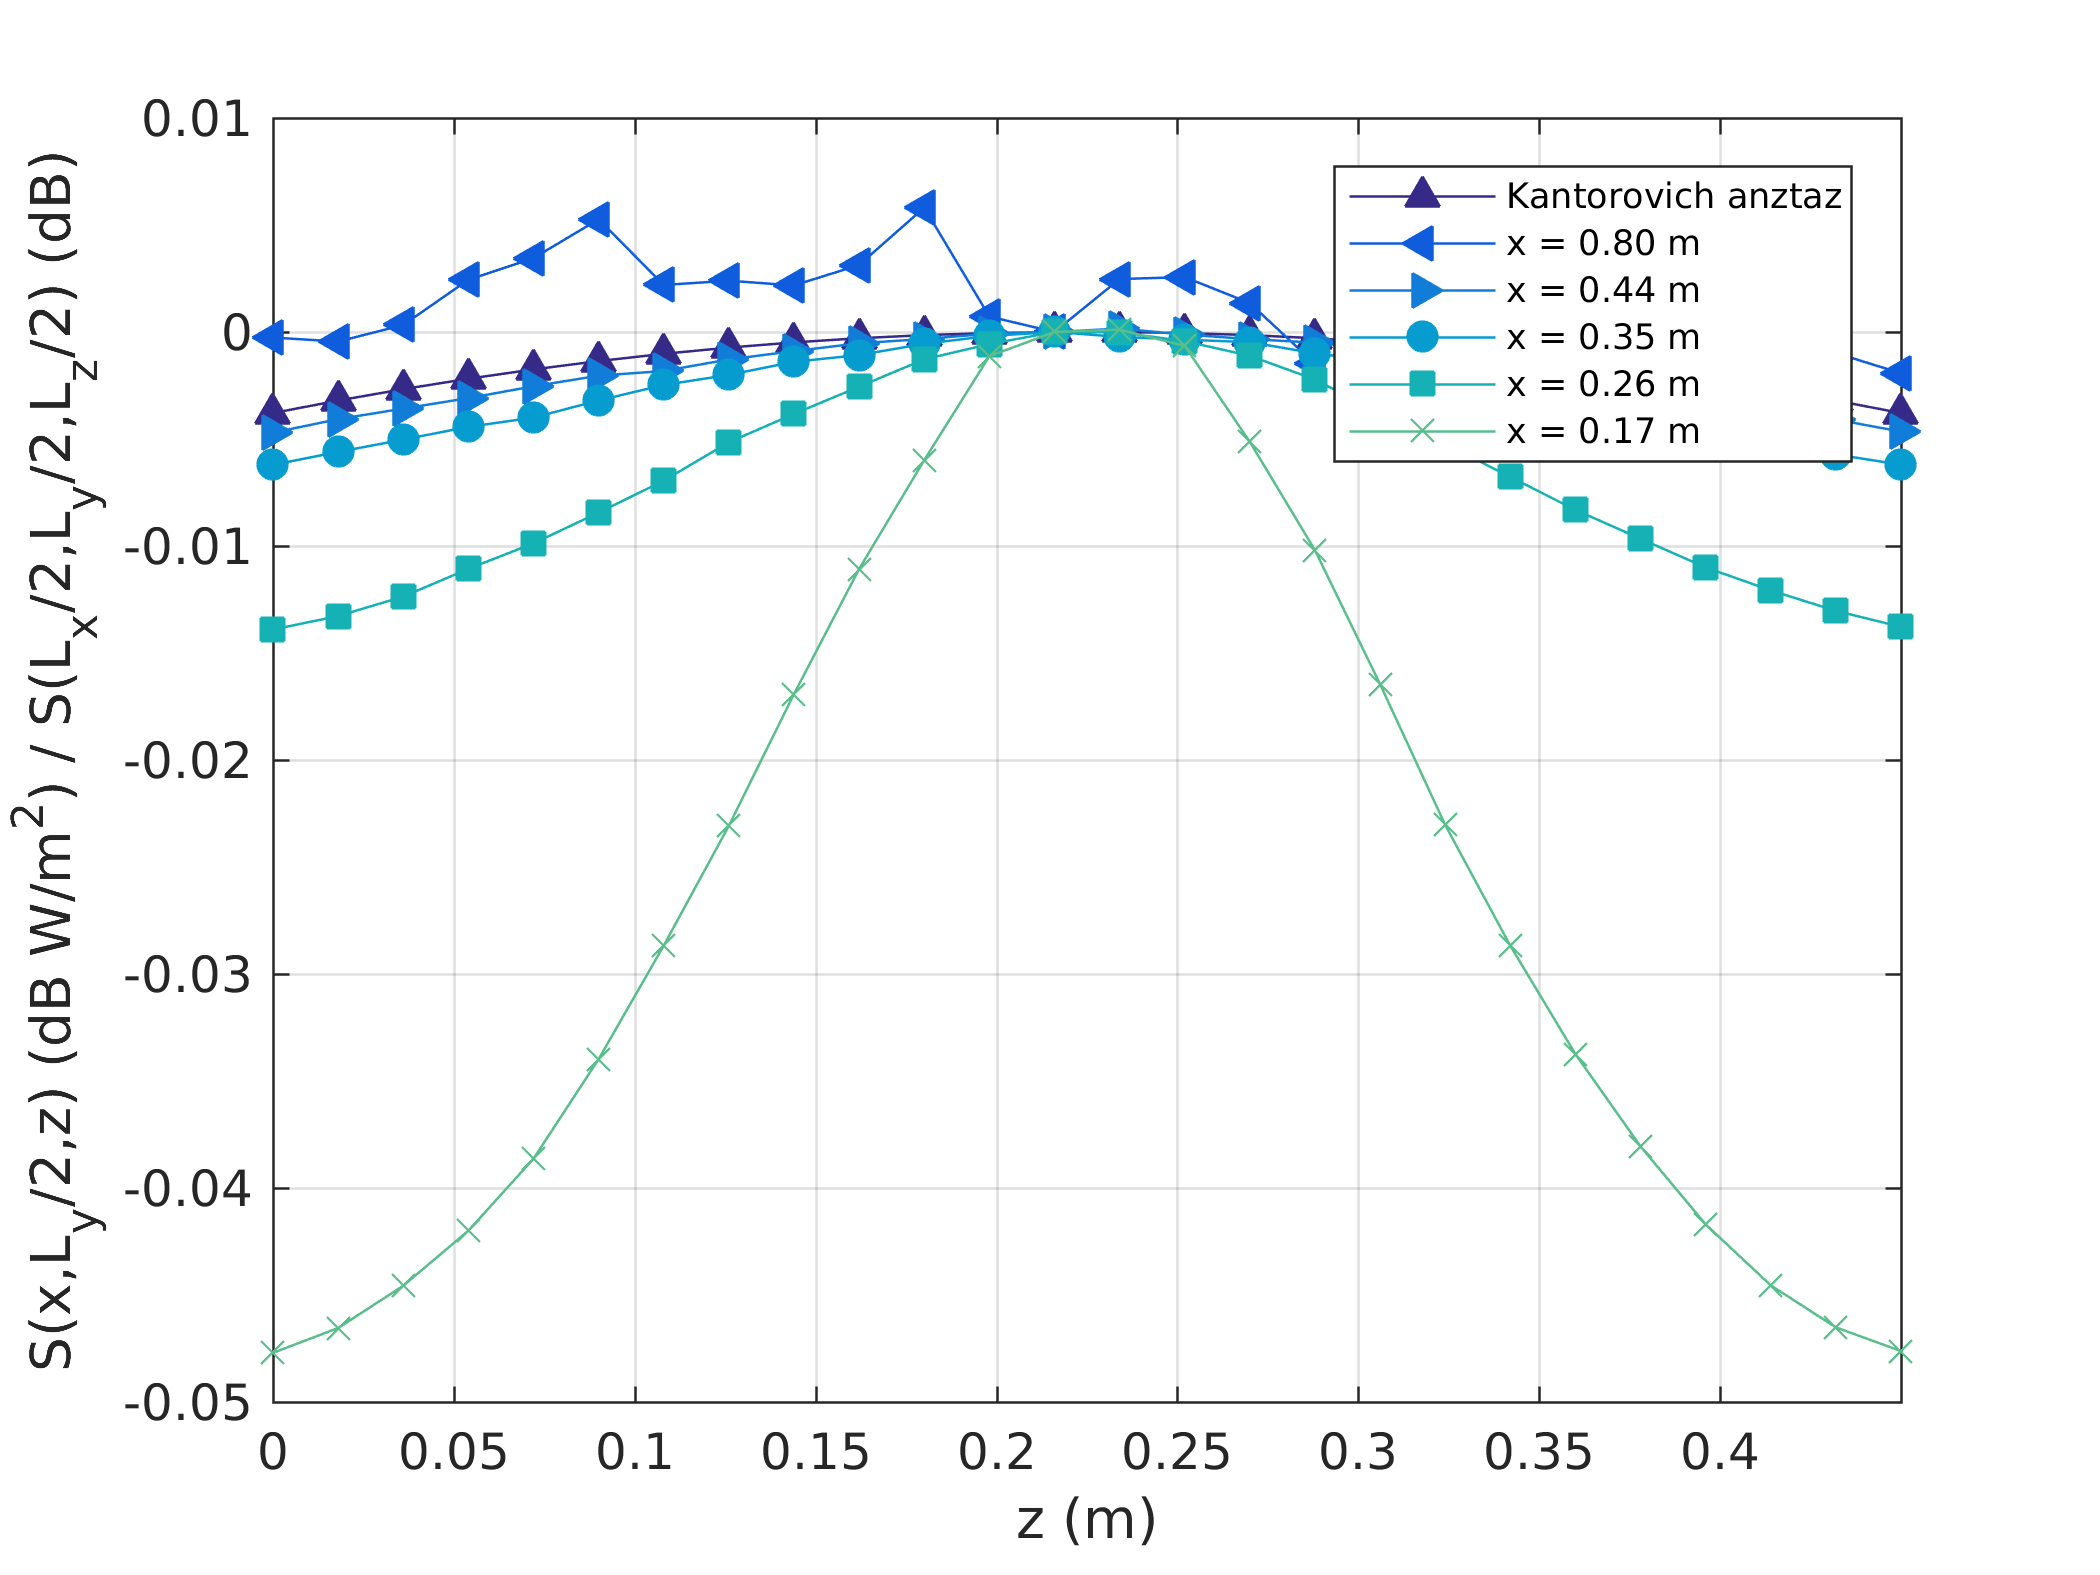
\includegraphics[width=0.6\linewidth]{figures/DDM-EEBC_3D_DL_PowerDensityProfileZ}\\
{\footnotesize (a)}\\
\vspace{2mm}
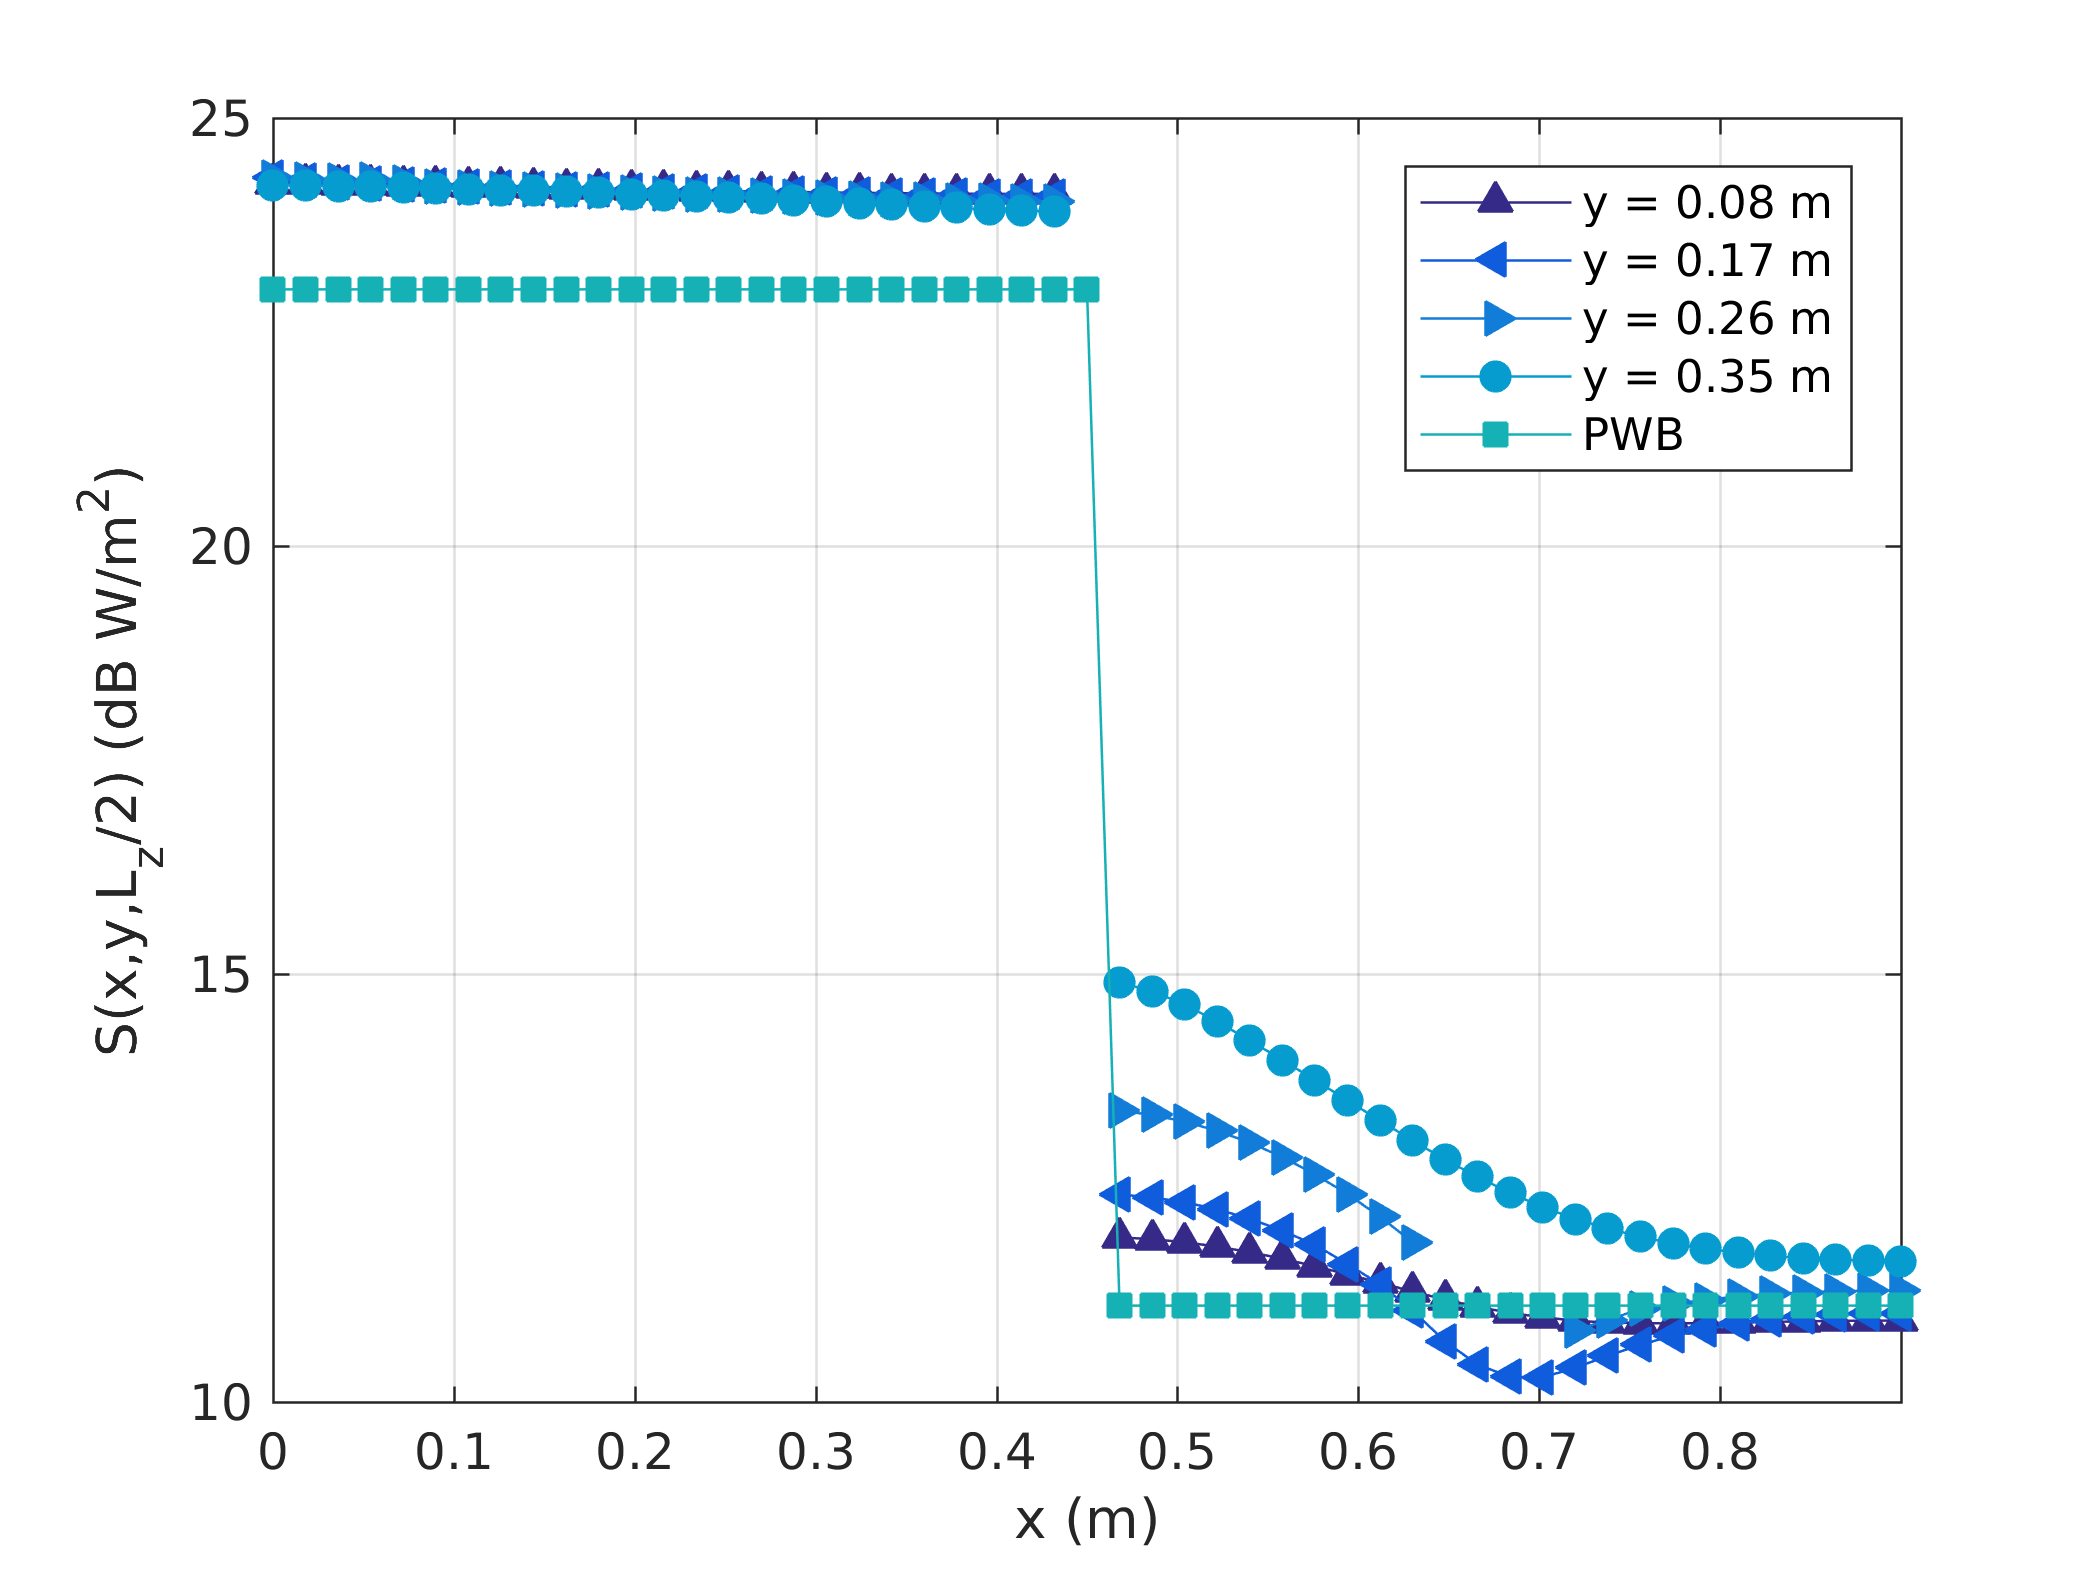
\includegraphics[width=0.6\linewidth]{figures/DDM-EEBC_3D_DL_PowerDensityProfileX}\\
{\footnotesize (b)}\\
\vspace{2mm}
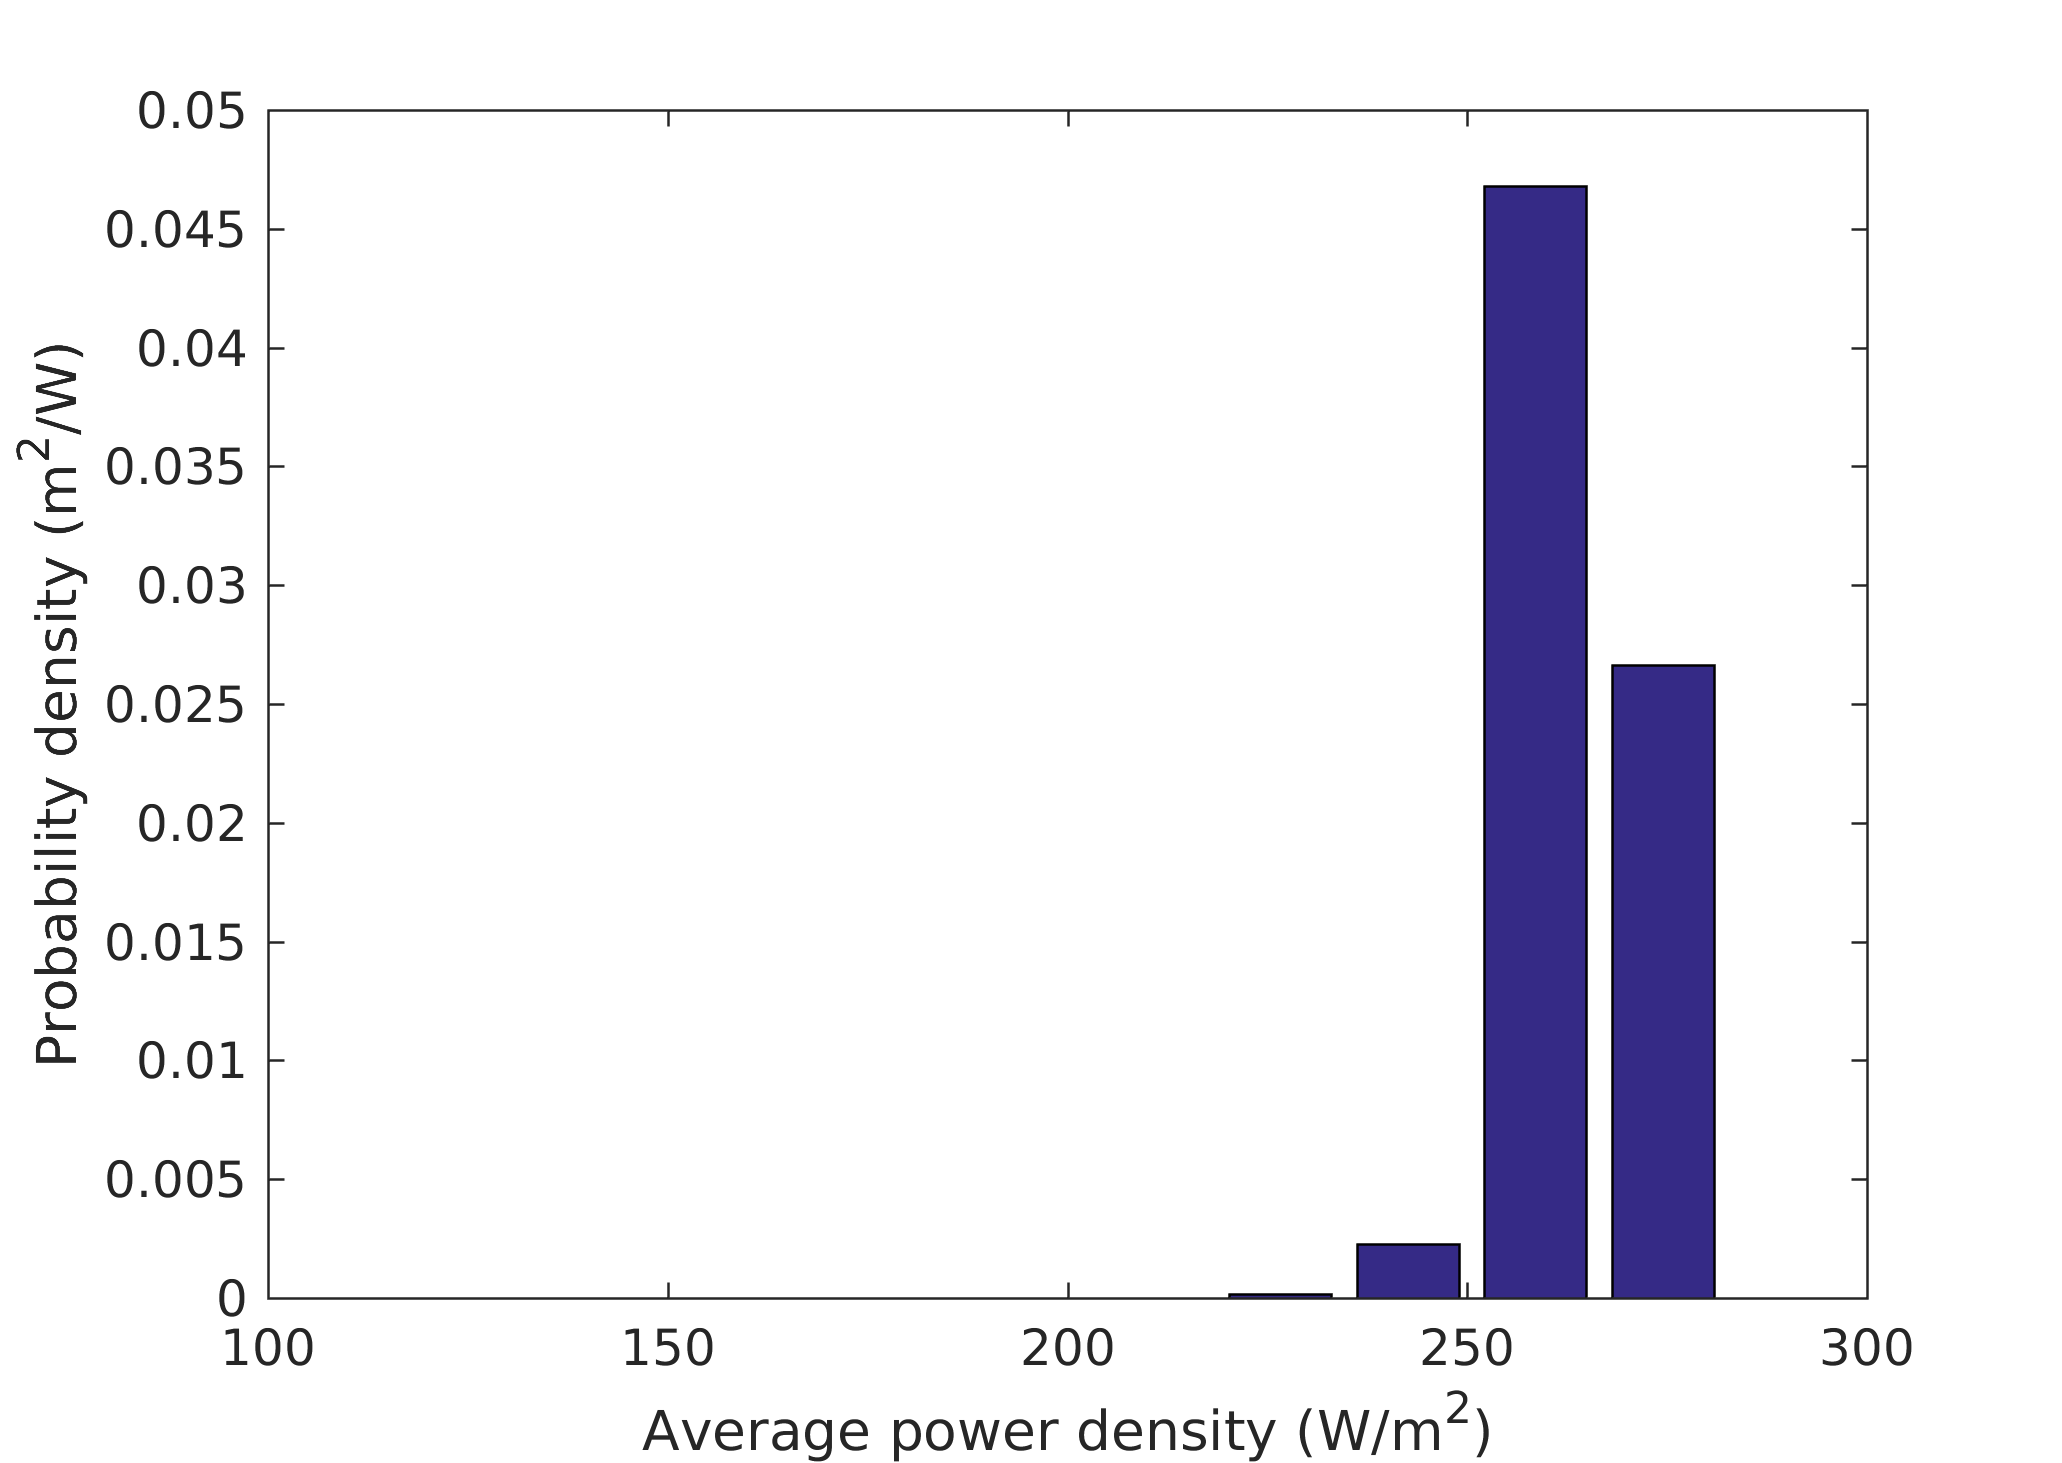
\includegraphics[width=0.45\linewidth]{figures/DDM-EEBC_3D_DL_PowerDensityPDF1}
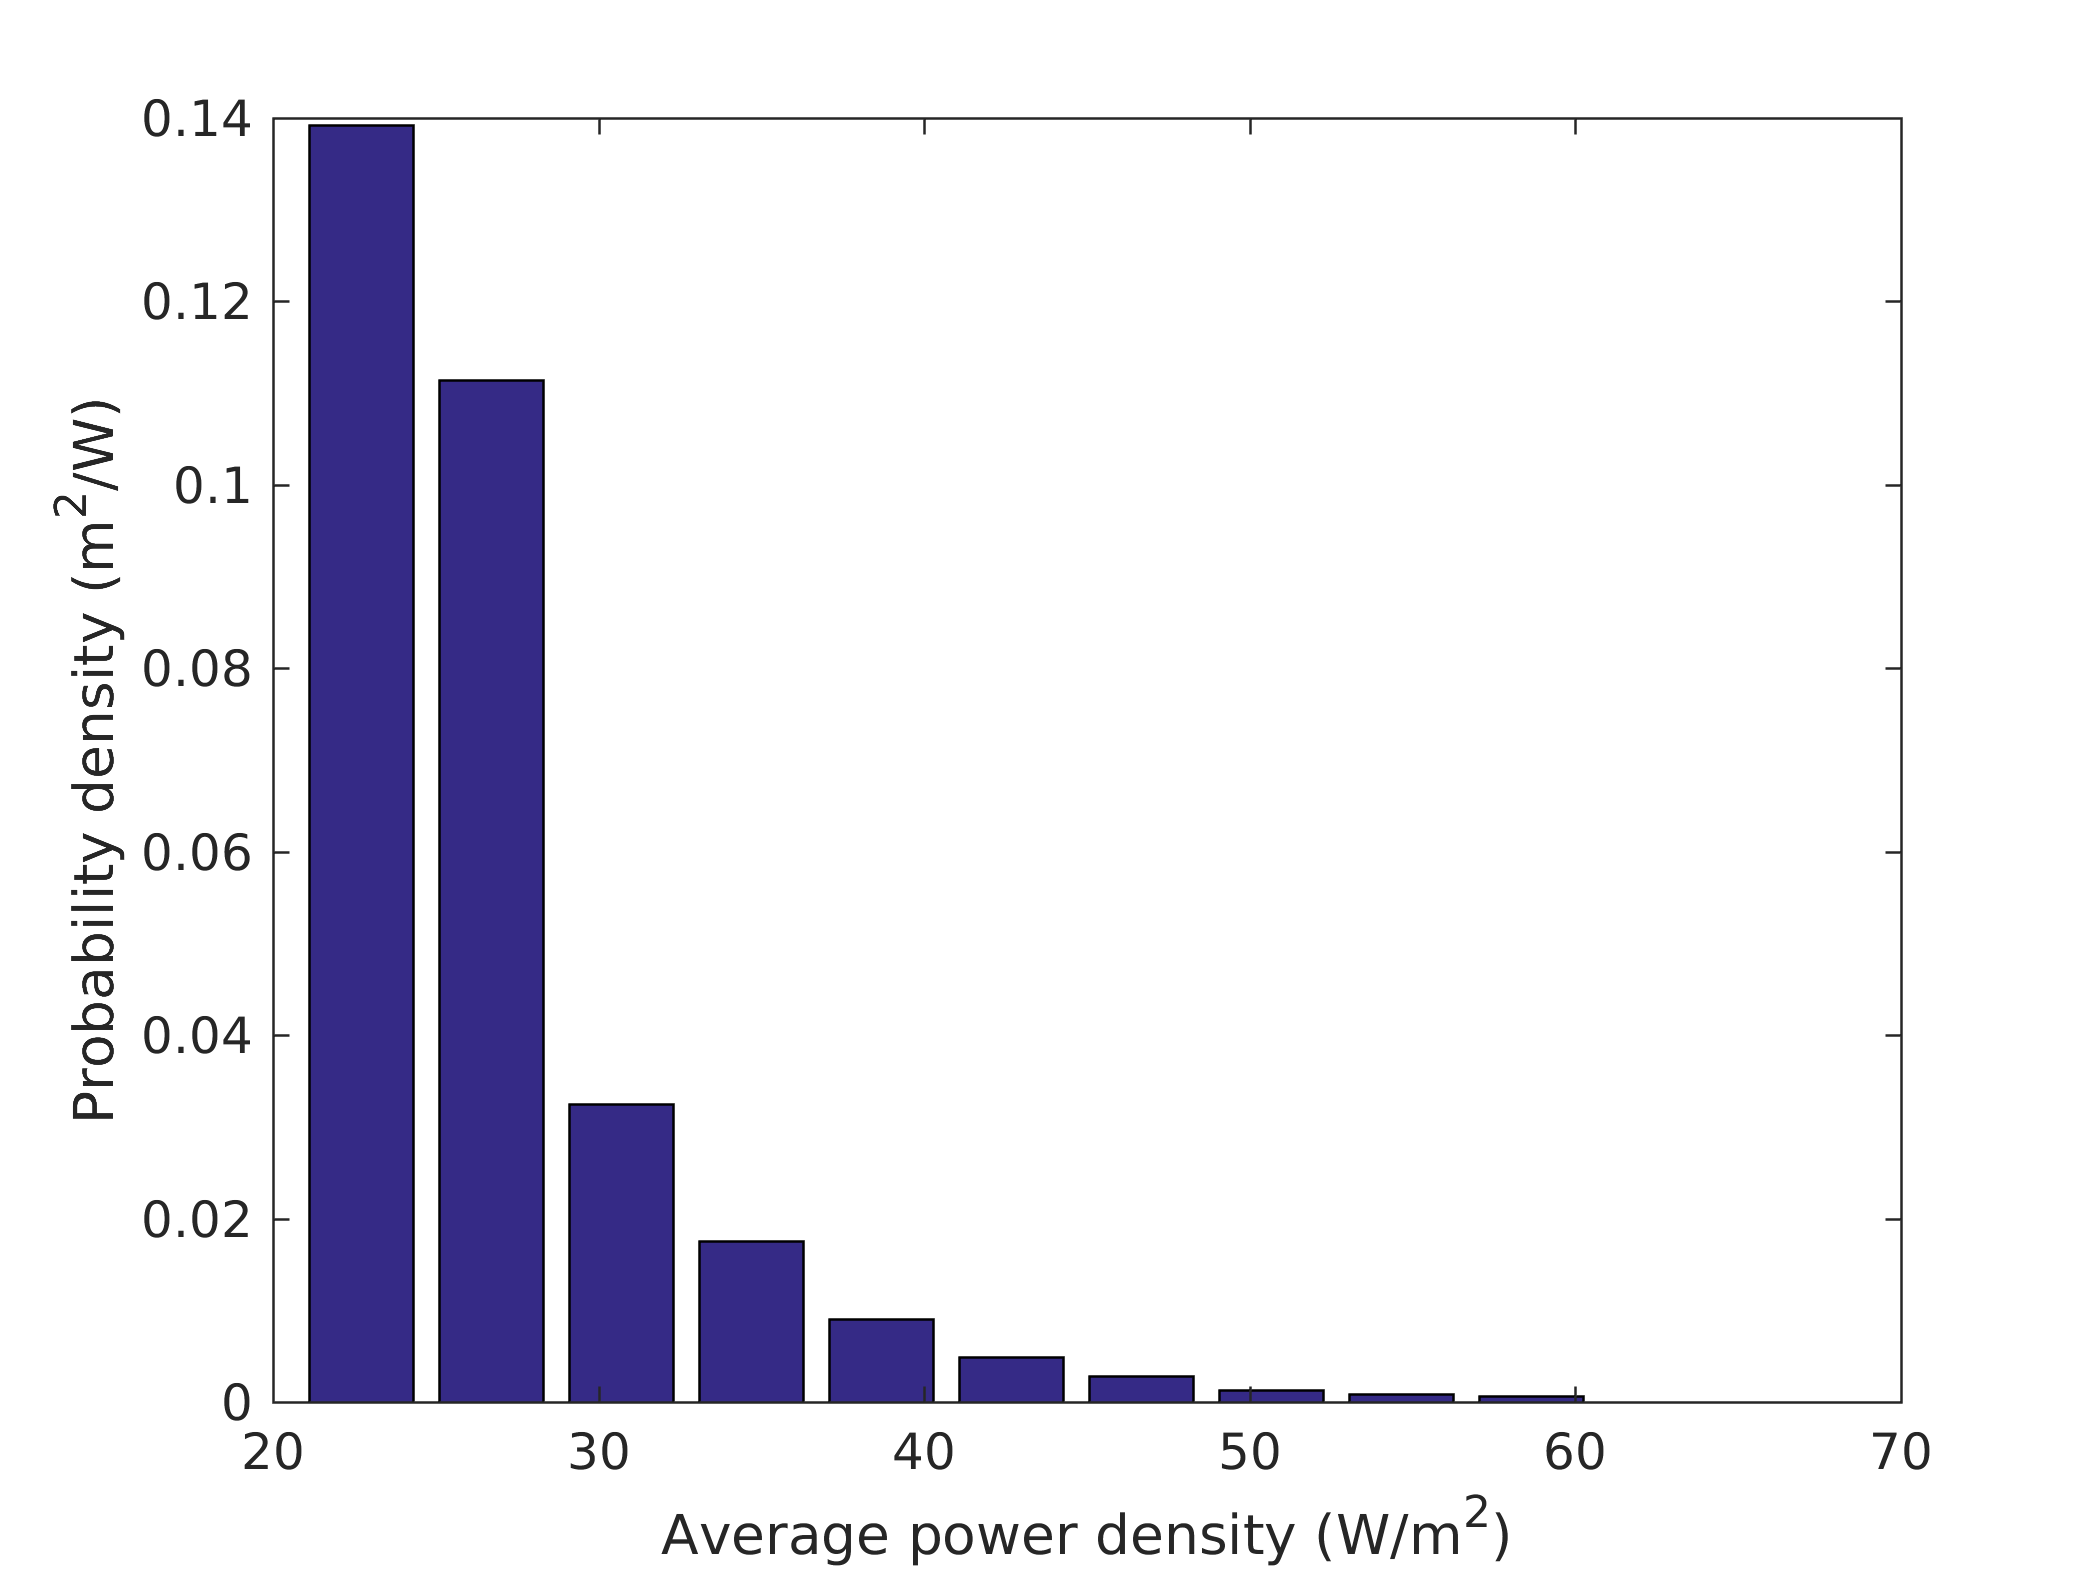
\includegraphics[width=0.45\linewidth]{figures/DDM-EEBC_3D_DL_PowerDensityPDF2}
\\
{\footnotesize (c)}\\
\vspace{-2mm}
\caption{\label{fg:partcylddm_profs} Dual domain EEBC EDM of the loaded partitioned cavity: (a) Normalised vertical profile of the power density; 
(b) Power density profile in the $x$-direction along the cavity centre; (c) PDF of the power density in the source cavity (left) and coupled cavity (right).}
\end{center}
\end{figure}

\begin{figure}[hp]
\begin{center}
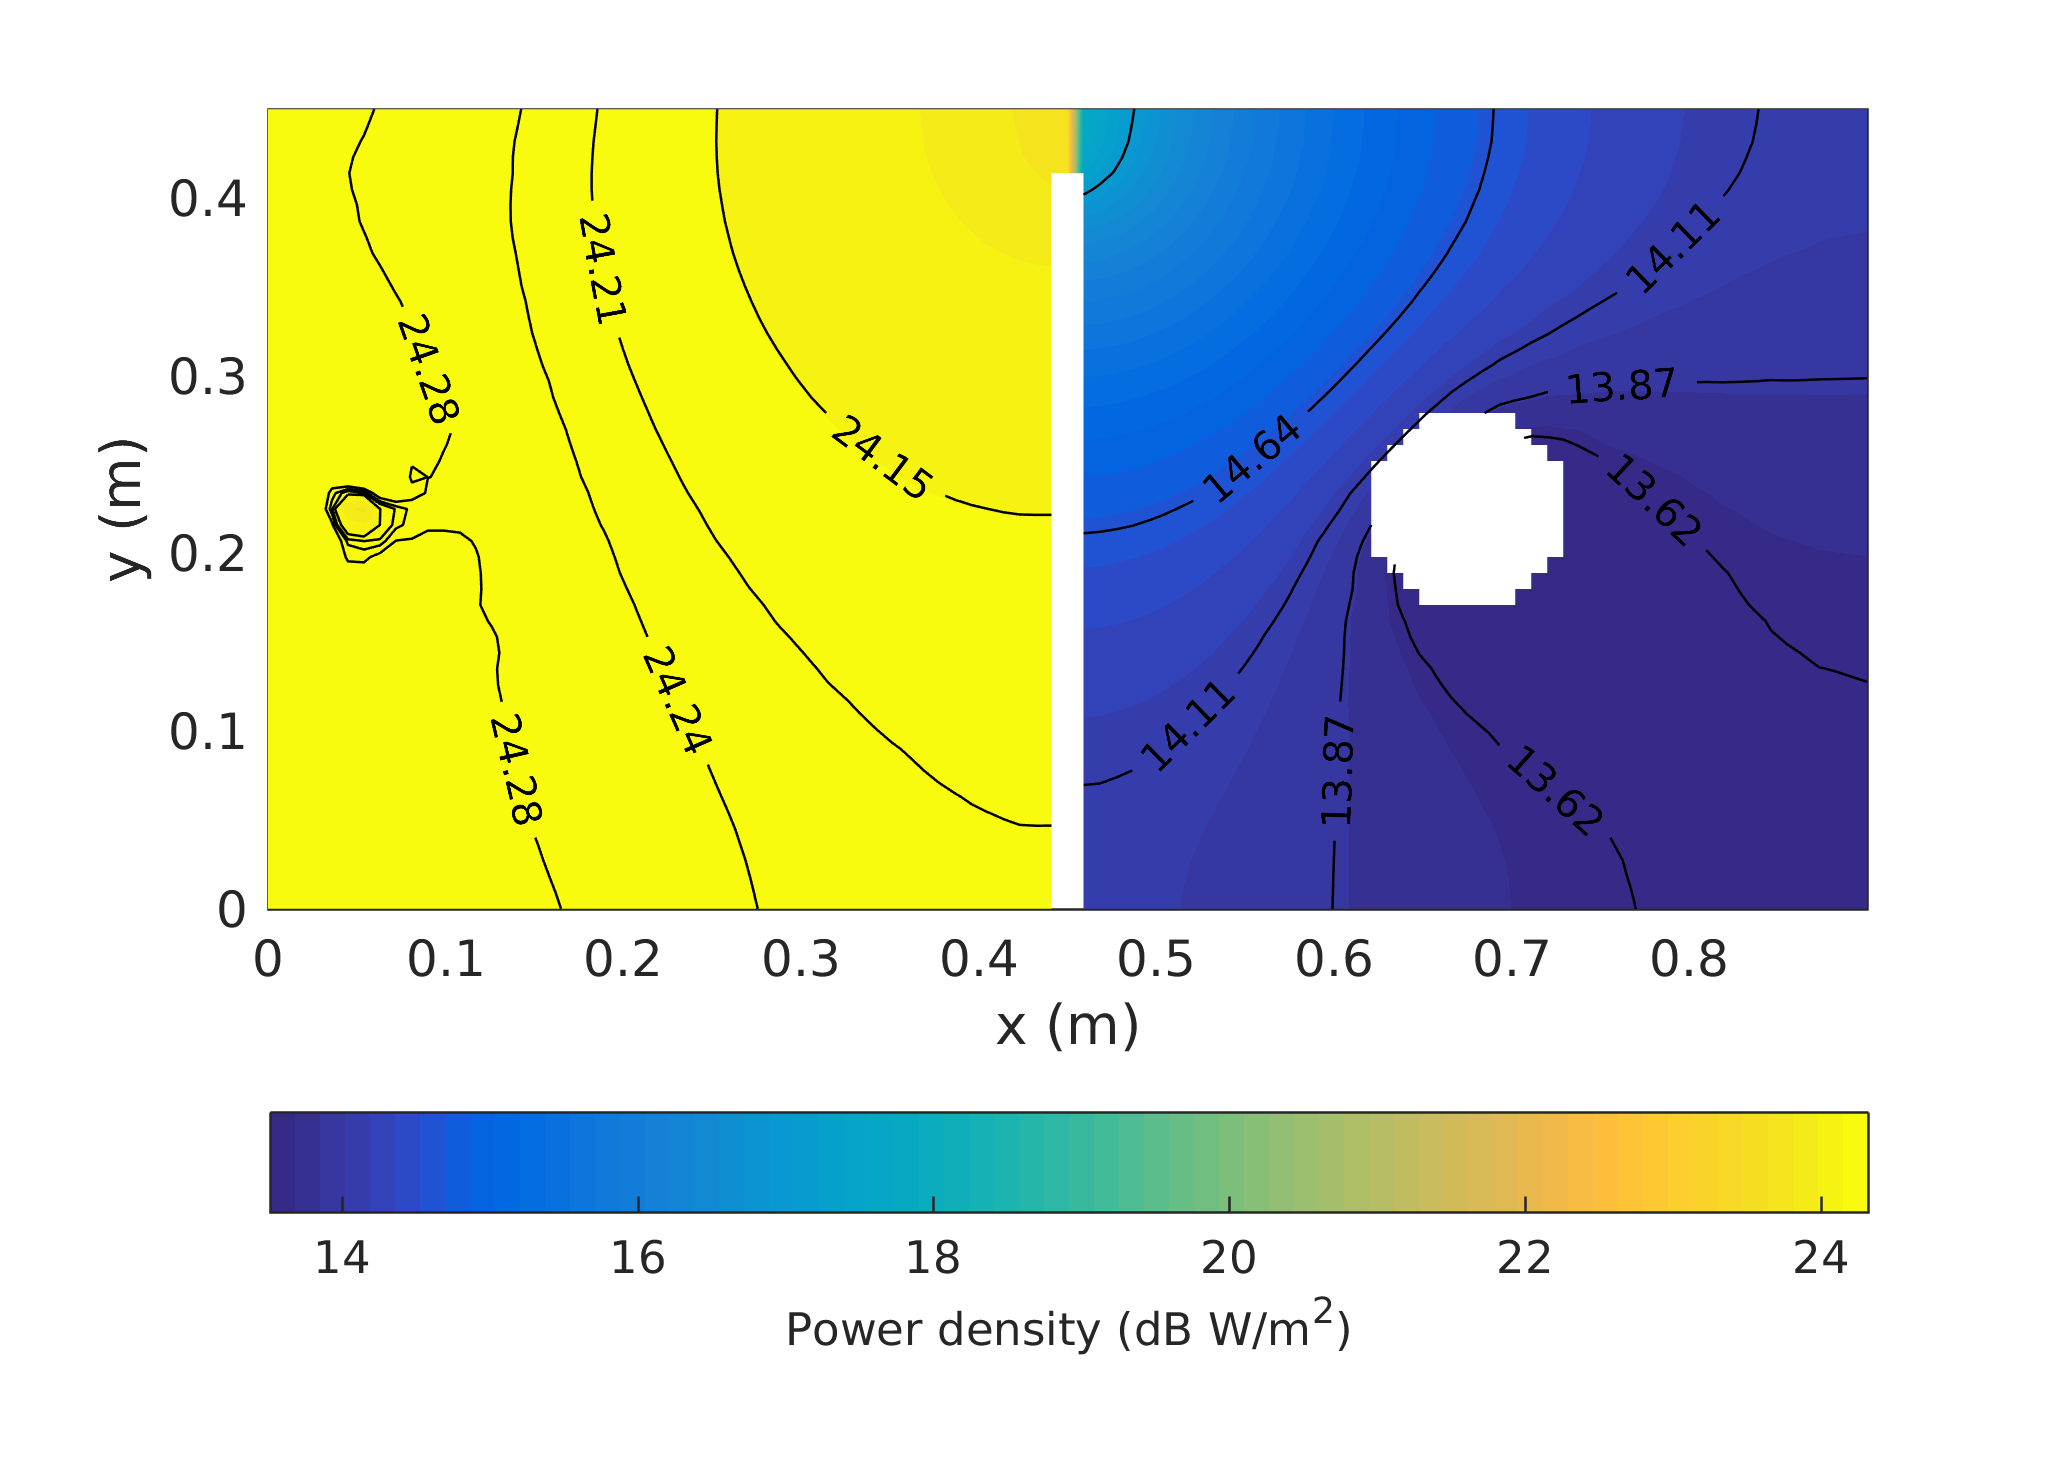
\includegraphics[trim={0 8mm 0 12mm},clip,width=0.52\linewidth]{figures/DDM-EEBC_3D_DL_PowerDensityMap}\\
{\footnotesize (a)}\\
\vspace{2mm}
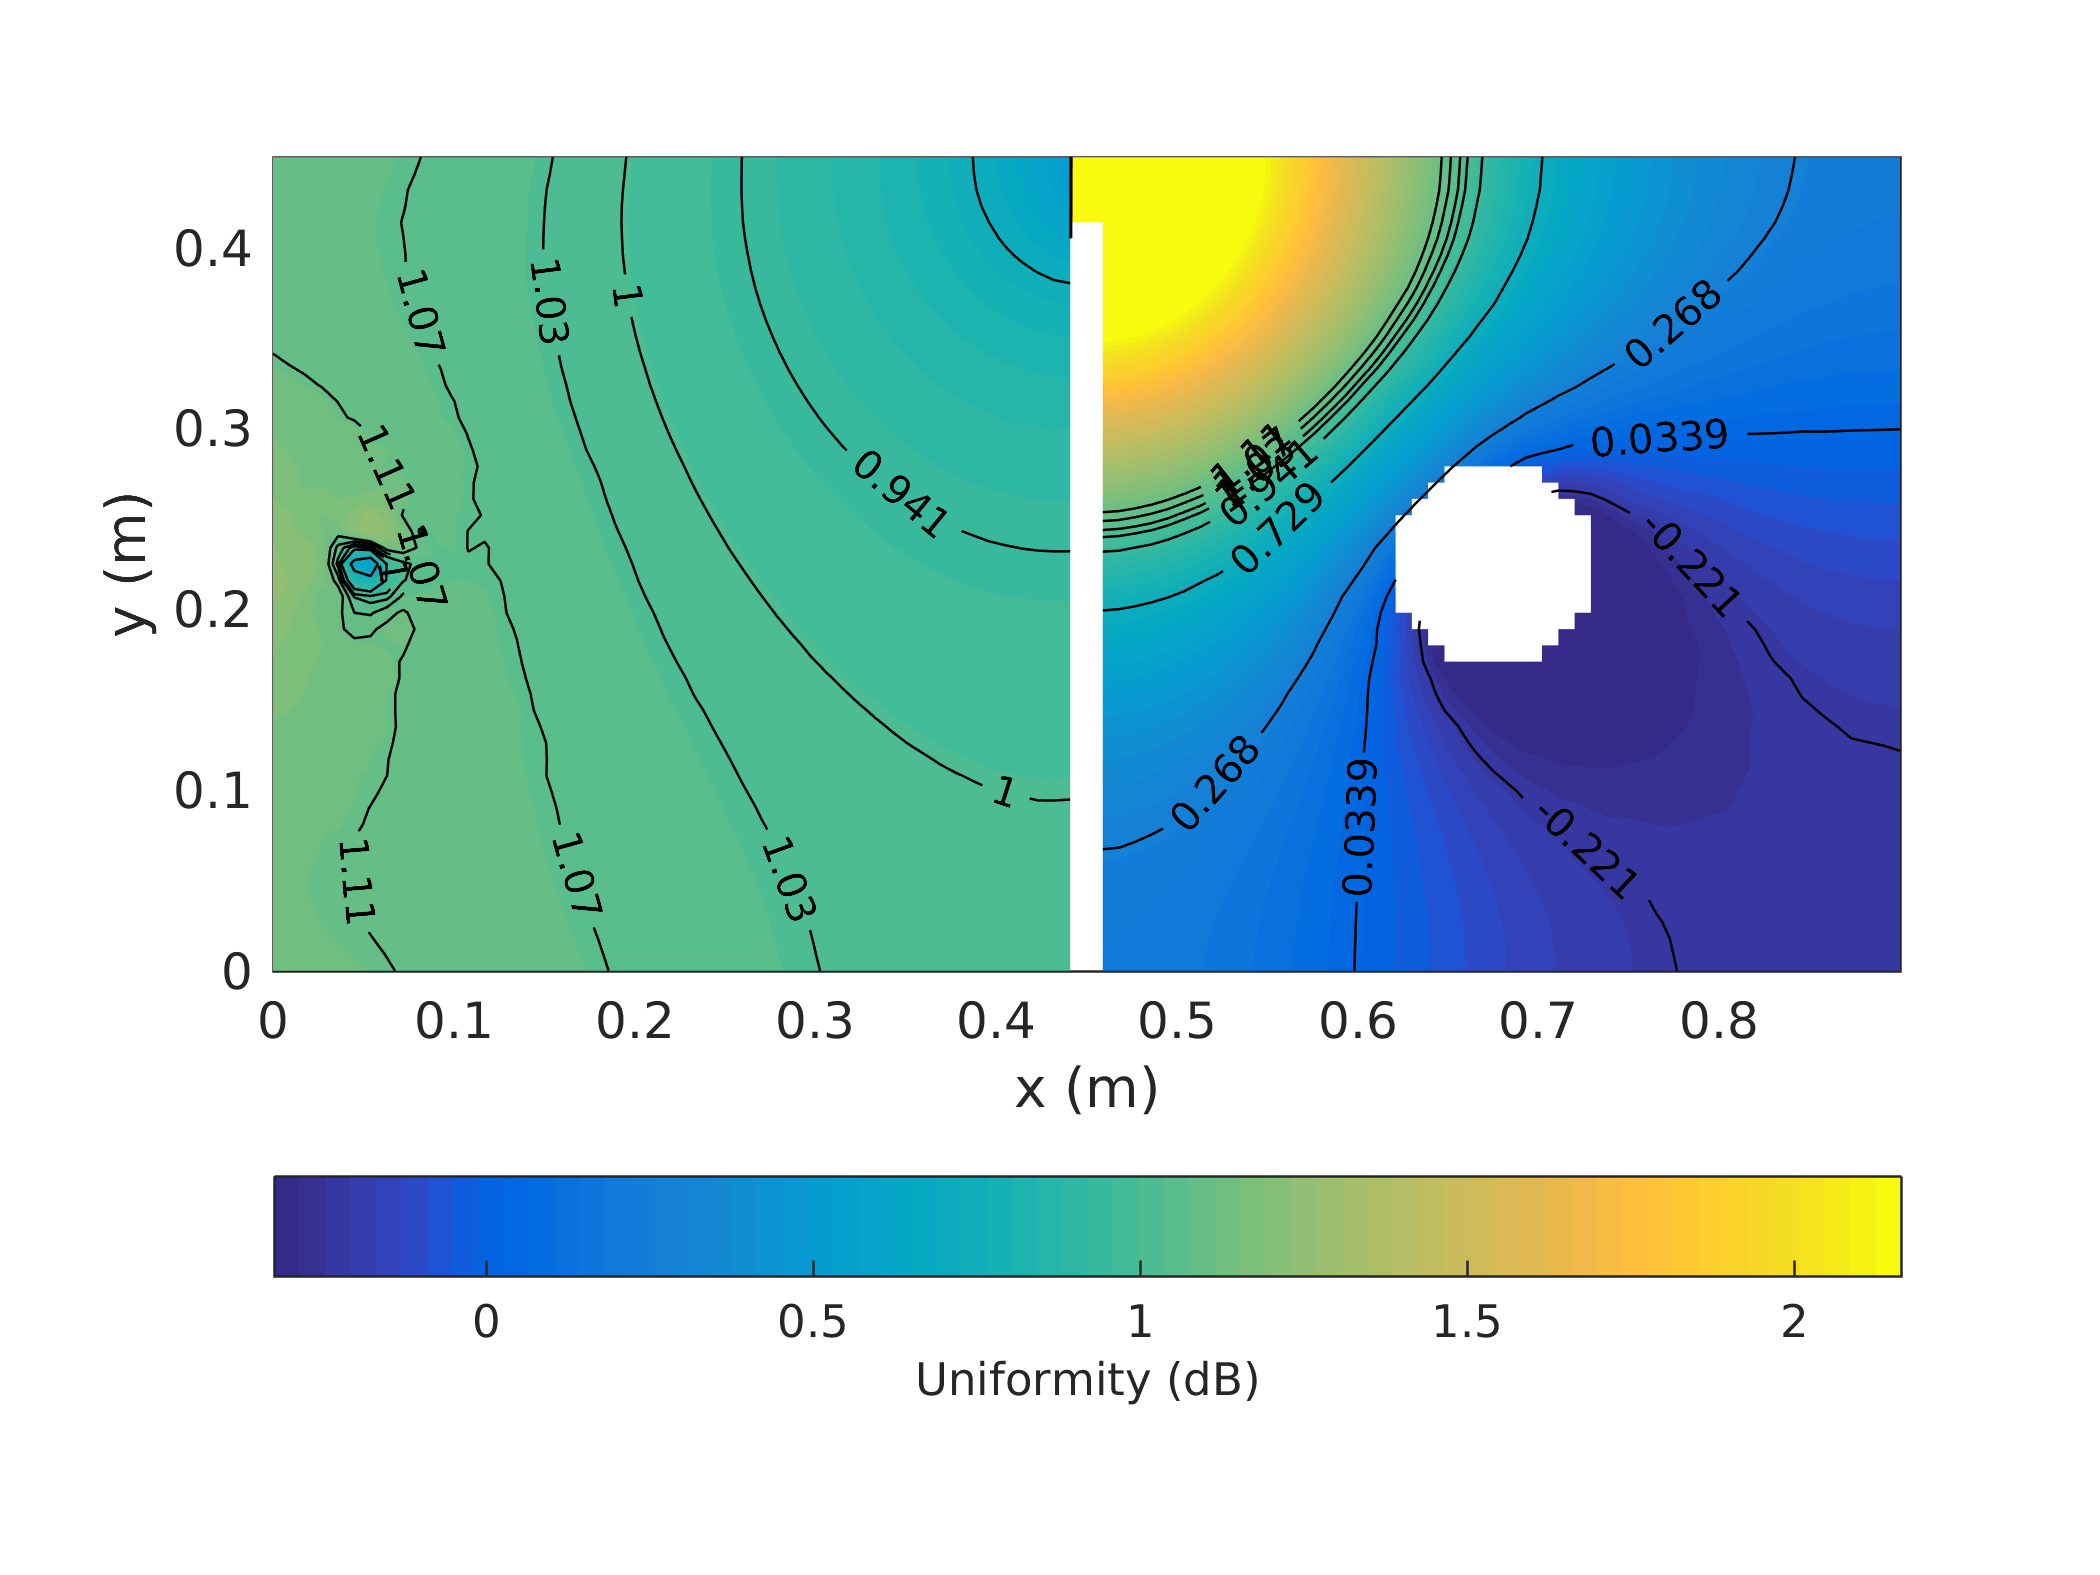
\includegraphics[trim={0 8mm 0 12mm},clip,width=0.52\linewidth]{figures/DDM-EEBC_3D_DL_EnergyDensityUniformityMap}\\
{\footnotesize (b)}\\
\vspace{2mm}
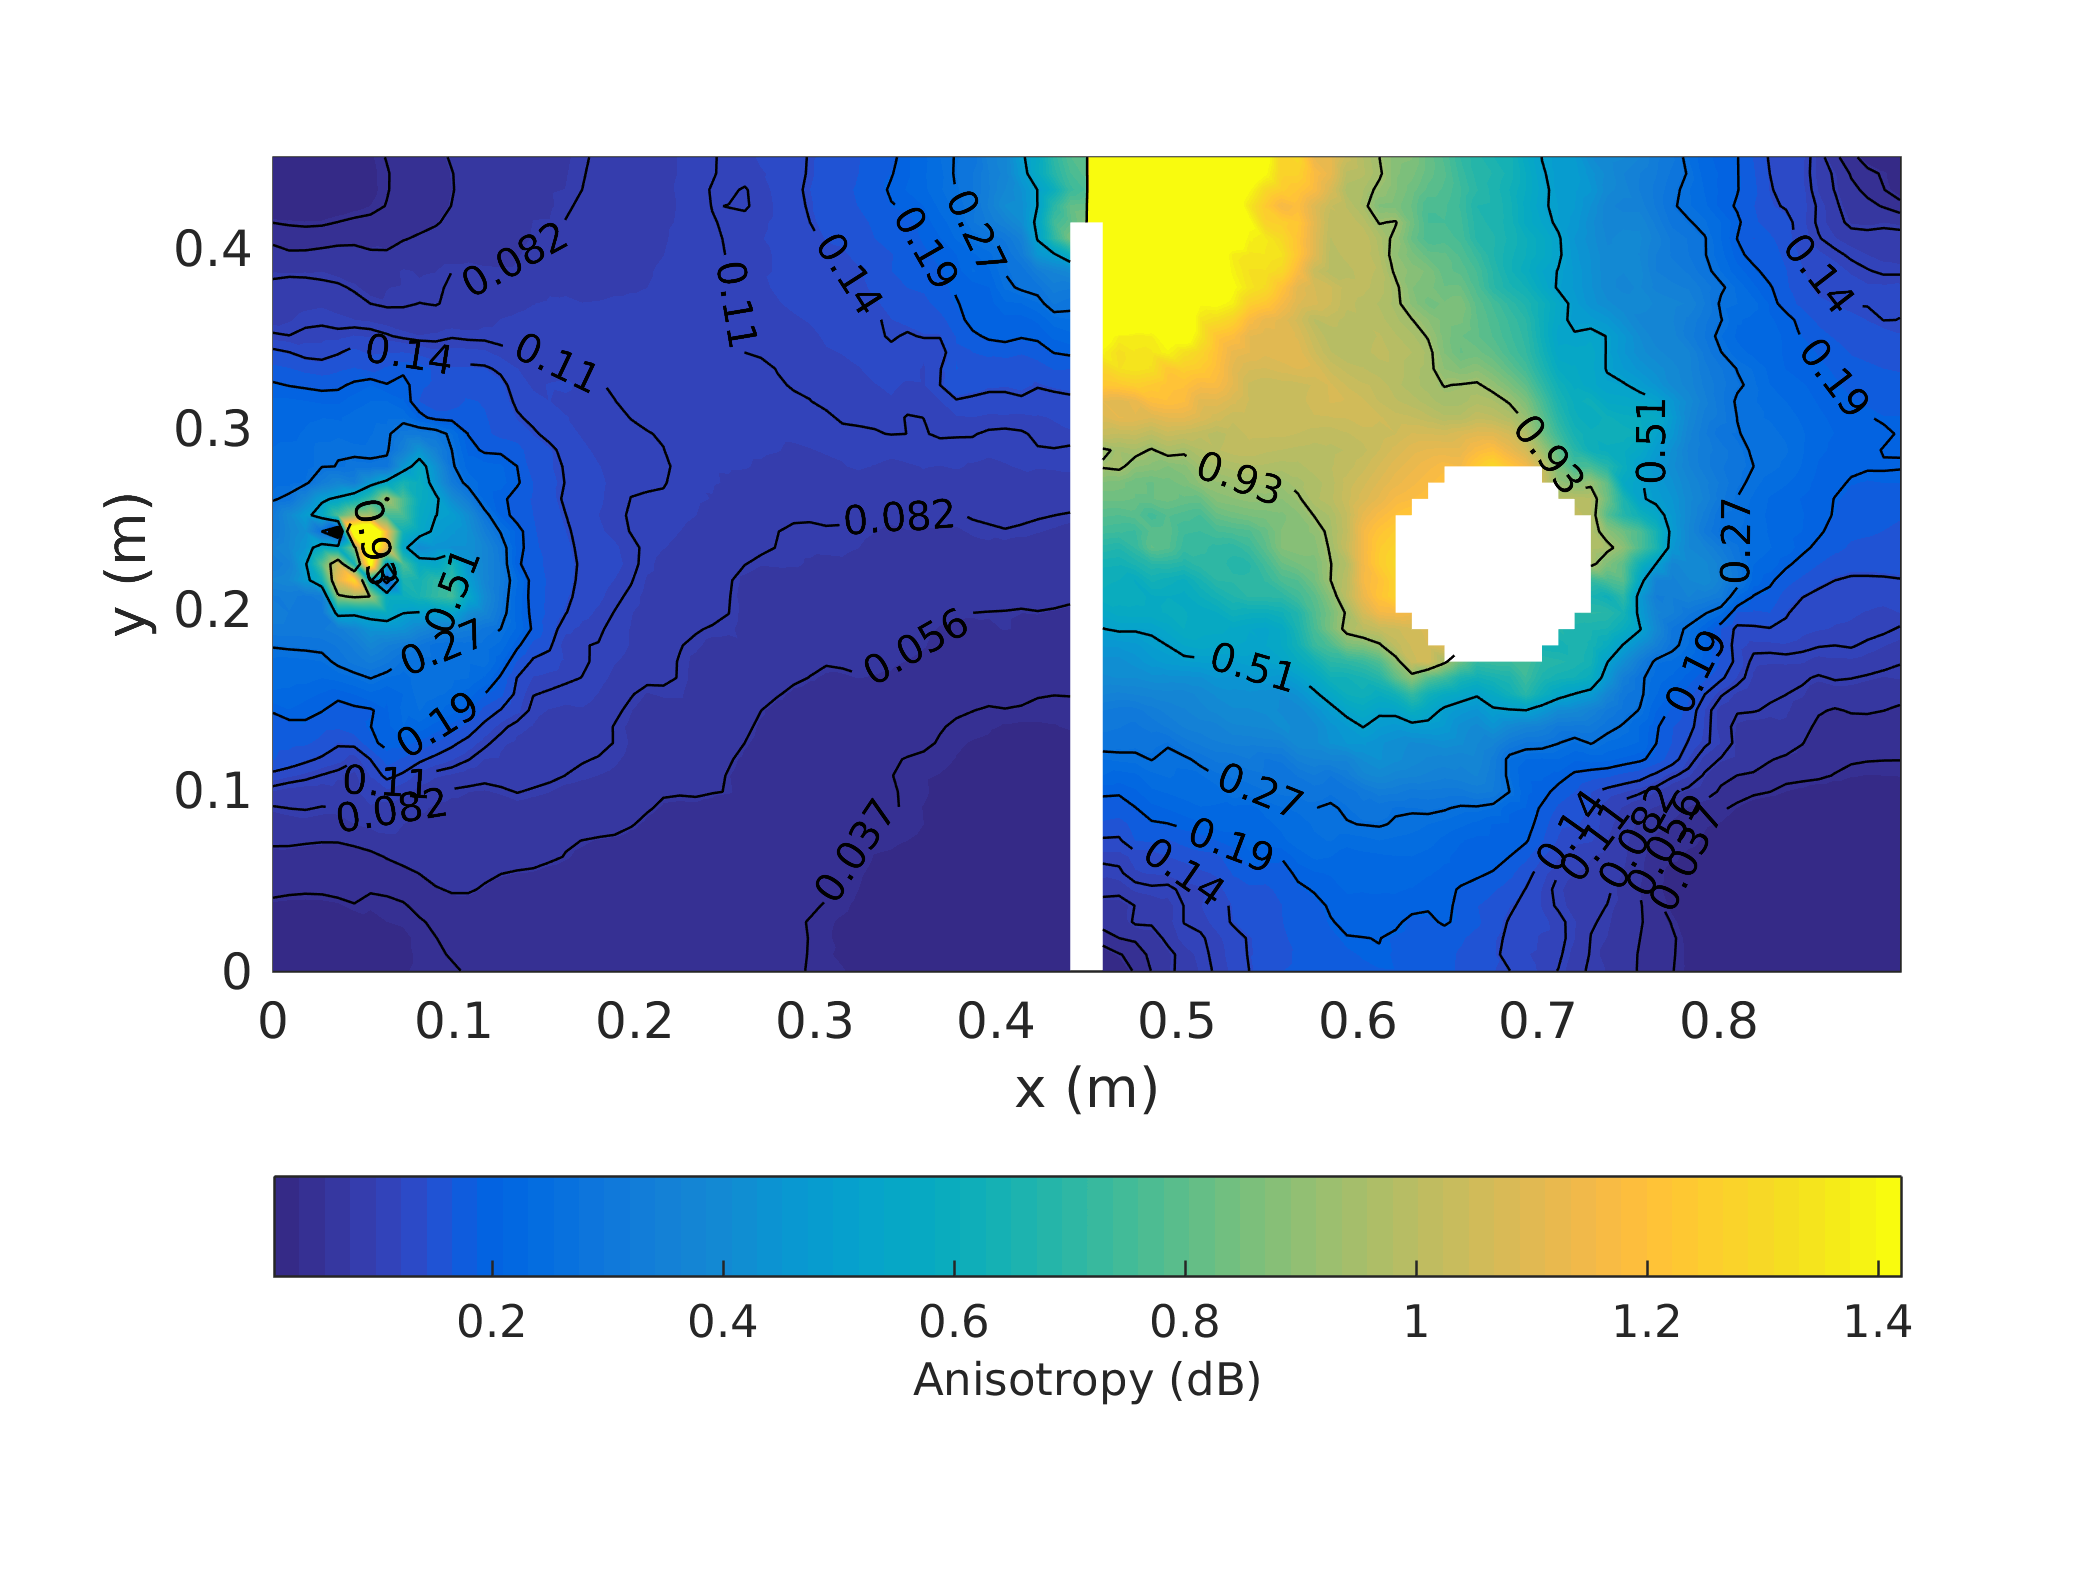
\includegraphics[trim={0 8mm 0 12mm},clip,width=0.52\linewidth]{figures/DDM-EEBC_3D_DL_EnergyDensityAnisotropyMap}\\
{\footnotesize (c)}\\
\vspace{2mm}
\includegraphics[trim={0 8mm 0 12mm},clip,width=0.52\linewidth]{figures/DDM-EEBC_3D_DL_EnergyDensityFluxMap}\\
{\footnotesize (d)}\\
\vspace{-2mm}
\caption{\label{fg:partcylddm_maps} Dual domain EEBC 3D EDM maps in the $z$-normal plane at the half height of the cavity for the 
loaded partitioned cavity: (a) Power density; (b) Energy density relative to the homogeneous PWB model;
(c) Anisotropy; (d) Energy density flux.}
\end{center}
\end{figure}

\clearpage

\subsection[Comparison to measurements]{Comparison to measurements}
\label{sc:res:meas}

Measurements of the power density in a physical implementation of the test-cases where reported in~\citep{Flintoft2017b}. 
In this section this measurement data is compared to the predictions of the 3D EDM. Since it is readily apparent that the 
SDM model of the partitioned cavity does not agree well with the measurement data only the 3D EEBC model results are 
considered. EDM results with two different EC models, Sabine and Jing and Xiang, are however shown. The comparisons
are made using the profile of the power density in the $x$ direction along the cavity.

Figure~\ref{fg:measprofssu} shows the power density comparison for the unloaded unpartitioned cavity. The measurement 
result exhibits significant statistical variation. The EDM results are at least consistent with the measurement data
in this case and no conclusion can be draw regarding the validity of the two EC models.

\begin{figure}[hp]
\begin{center}
\includegraphics[width=0.6\linewidth]{figures/SDM_3D_SU_PowerDensityProfileXMeas}\\
{\footnotesize (a)}\\
\vspace{2mm}
\includegraphics[width=0.6\linewidth]{figures/SDM_3D_SU_PowerDensityProfileXMeas_JX}\\
{\footnotesize (b)}\\
\vspace{-2mm}
\caption{\label{fg:measprofssu} Power density profile in the $x$-direction along the cavity centre comparing
the 3D EDM of the single unloaded cavity and measurement~\citep{Flintoft2017b}: (a) Sabine EC; (b) Jing and Xiang EC.}
\end{center}
\end{figure}

Figure~\ref{fg:measprofssl} shows the power density comparison for the loaded unpartitioned cavity. While again the 
measurement has significant statistical variation, the general trend of the measurement data, a reduction in level
with increasing distance from the source, is consistent with the EDM results. While neither EC model matches 
the overall trend in the measurement across the full length of the cavity, the measurement data is generally within
the range of the two models, favouring te Sabine EC model closer to the source and the Jing and Xiang model at the other
end of the cavity.

\begin{figure}[hp]
\begin{center}
\includegraphics[width=0.6\linewidth]{figures/SDM_3D_SL_PowerDensityProfileXMeas}\\
{\footnotesize (a)}\\
\vspace{2mm}
\includegraphics[width=0.6\linewidth]{figures/SDM_3D_SL_PowerDensityProfileXMeas_JX}\\
{\footnotesize (b)}\\
\vspace{-2mm}
\caption{\label{fg:measprofssl} Power density profile in the $x$-direction along the cavity centre comparing
the 3D EDM of the single loaded cavity and measurement~\citep{Flintoft2017b}: (a) Sabine EC; (b) Jing and Xiang EC.}
\end{center}
\end{figure}

The power density comparison for the unloaded partitioned cavity is shown in Figure~\ref{fg:measprofsdu}.
Since the loss is low the Sabine and Jing and Xiang EC models give very similar results. The agreement with
the measurement data is good, though the EDM seems to overestimate the power density in the coupled cavity.
The statistical variation of the measurement data is a least consistent with a relatively uniform level in
each sub-cavity.

\begin{figure}[hp]
\begin{center}
\includegraphics[width=0.6\linewidth]{figures/DDM-EEBC_3D_DU_PowerDensityProfileXMeas}\\
{\footnotesize (a)}\\
\vspace{2mm}
\includegraphics[width=0.6\linewidth]{figures/DDM-EEBC_3D_DU_PowerDensityProfileXMeas_JX}\\
{\footnotesize (b)}\\
\vspace{-2mm}
\caption{\label{fg:measprofsdu} Power density profile in the $x$-direction along the cavity centre comparing
the 3D DDM EEBC EDM of the dual unloaded cavity and measurement~\citep{Flintoft2017b}: (a) Sabine EC; (b) Jing and Xiang EC.}
\end{center}
\end{figure}

Figure~\ref{fg:measprofsdl} shows the power density comparison for the loaded partitioned cavity. In this case it appears
that the simulation using the Jing and Xiang EC gives significantly better agreement with the measurement data than
the simulation using the Sabine EC model. The Sabine model appears to under-estimate the level difference between
the cavities and shows less variation in the $y$ direction than the measurement data. The Jing and Xiang EC simulation 
gives a much better estimate of the level difference and while it still under-estimates the variation in the $y$-direction
compared to the measurement data, it is closer to the measurement than the prediction of the Sabine EC simulation.

\begin{figure}[hp]
\begin{center}
\includegraphics[width=0.6\linewidth]{figures/DDM-EEBC_3D_DL_PowerDensityProfileXMeas}\\
{\footnotesize (a)}\\
\vspace{2mm}
\includegraphics[width=0.6\linewidth]{figures/DDM-EEBC_3D_DL_PowerDensityProfileXMeas_JX}\\
{\footnotesize (b)}\\
\vspace{-2mm}
\caption{\label{fg:measprofsdl} Power density profile in the $x$-direction along the cavity centre comparing
the 3D DDM EEBC EDM of the dual loaded cavity and measurement~\citep{Flintoft2017b}: (a) Sabine EC; (b) Jing and Xiang EC.}
\end{center}
\end{figure}

\subsection[Parametric study]{Parametric study}
\label{sc:res:para}

All the EDM simulations so far have assumed that the domain boundaries have completely diffuse reflections,
corresponding to $\kappa=1$ in~(\ref{eq:kappa}). In this section a comparison is made between the measurement
data from~\citep{Flintoft2017b} and the 3D EDM (using the EEBC for the partitioned cavity and Jing and Xiang EC)
with the specularity parameter $\kappa$ taking values of 0.5, 0.75, 1, 1.5 and 2. Whilst in the acoustics
diffusion model $\kappa$ is supposed to quantify the effect of specular reflections on the diffusivity, in
more general terms it represents variations in the MFP from the value given by that in~(\ref{eq:mfp}).

Figure~\ref{fg:measprofssuk} shows the parametric sweep for the empty unpartitioned cavity. In this case there
is little variation with $\kappa$ and the statistical variation in the measurement data is too high to draw any
conclusions. Figure~\ref{fg:measprofsslk} show the sweep for the loaded unpartitioned cavity. This shows that
increasing $\kappa$ tends to reduce both the overall level and variability in the power density in the cavity. 
The best comparison to the measurement data would appear to be achieved with $\kappa$ in the range 0.5 to 0.75, 
with the lower value favoured.

\begin{figure}[hp]
\begin{center}
\includegraphics[width=0.49\linewidth]{figures/SDM_3D_SU_PowerDensityProfileXMeas_JX_k0_5}
\includegraphics[width=0.49\linewidth]{figures/SDM_3D_SU_PowerDensityProfileXMeas_JX_k0_75}\\
{\footnotesize (a)\hspace{75mm}(b)}\\
\includegraphics[width=0.5\linewidth]{figures/SDM_3D_SU_PowerDensityProfileXMeas_JX_k1_0}\\
{\footnotesize (c)}\\
\includegraphics[width=0.49\linewidth]{figures/SDM_3D_SU_PowerDensityProfileXMeas_JX_k1_5}
\includegraphics[width=0.49\linewidth]{figures/SDM_3D_SU_PowerDensityProfileXMeas_JX_k2_0}\\
{\footnotesize (d)\hspace{75mm}(e)}\\
\vspace{-2mm}
\caption{\label{fg:measprofssuk} Power density profile in the $x$-direction along the cavity centre comparing
the 3D EDM of the single unloaded cavity and measurement~\citep{Flintoft2017b}: (a) $\kappa=1/2$; (b) $\kappa=3/4$;
(c) $\kappa=1$; (d) $\kappa=3/2$; (e) $\kappa=2$.}
\end{center}
\end{figure}

\begin{figure}[hp]
\begin{center}
\includegraphics[width=0.49\linewidth]{figures/SDM_3D_SL_PowerDensityProfileXMeas_JX_k0_5}
\includegraphics[width=0.49\linewidth]{figures/SDM_3D_SL_PowerDensityProfileXMeas_JX_k0_75}\\
{\footnotesize (a)\hspace{75mm}(b)}\\
\includegraphics[width=0.5\linewidth]{figures/SDM_3D_SL_PowerDensityProfileXMeas_JX_k1_0}\\
{\footnotesize (c)}\\
\includegraphics[width=0.49\linewidth]{figures/SDM_3D_SL_PowerDensityProfileXMeas_JX_k1_5}
\includegraphics[width=0.49\linewidth]{figures/SDM_3D_SL_PowerDensityProfileXMeas_JX_k2_0}\\
{\footnotesize (d)\hspace{75mm}(e)}\\
\vspace{-2mm}
\caption{\label{fg:measprofsslk} Power density profile in the $x$-direction along the cavity centre comparing
the 3D EDM of the single loaded cavity and measurement~\citep{Flintoft2017b}: (a) $\kappa=1/2$; (b) $\kappa=3/4$;
(c) $\kappa=1$; (d) $\kappa=3/2$; (e) $\kappa=2$.}
\end{center}
\end{figure}

The parametric sweep for the empty partitioned cavity is shown in Figure~\ref{fg:measprofsduk}. As for 
the unloaded unpartitioned cavity the effect of $\kappa$ is fairly small; however, lower values tend to
increase the level difference and variability which is again more consistent with the measurement 
results. Figure~\ref{fg:measprofsdlk} shows the sweep for the loaded partitioned cavity. The general
behaviour is the same, with reducing $\kappa$ increasing the level difference between the sub-cavities
and increasing the variability within each sub-cavity. The best agreement with the measurement
data is achieved with $\kappa\approx 0.5$.

\begin{figure}[hp]
\begin{center}
\includegraphics[width=0.49\linewidth]{figures/DDM-EEBC_3D_DU_PowerDensityProfileXMeas_JX_k0_5}
\includegraphics[width=0.49\linewidth]{figures/DDM-EEBC_3D_DU_PowerDensityProfileXMeas_JX_k0_75}\\
{\footnotesize (a)\hspace{75mm}(b)}\\
\includegraphics[width=0.5\linewidth]{figures/DDM-EEBC_3D_DU_PowerDensityProfileXMeas_JX_k1_0}\\
{\footnotesize (c)}\\
\includegraphics[width=0.49\linewidth]{figures/DDM-EEBC_3D_DU_PowerDensityProfileXMeas_JX_k1_5}
\includegraphics[width=0.49\linewidth]{figures/DDM-EEBC_3D_DU_PowerDensityProfileXMeas_JX_k2_0}\\
{\footnotesize (d)\hspace{75mm}(e)}\\
\vspace{-2mm}
\caption{\label{fg:measprofsduk} Power density profile in the $x$-direction along the cavity centre comparing
the 3D EDM of the dual unloaded cavity and measurement~\citep{Flintoft2017b}: (a) $\kappa=1/2$; (b) $\kappa=3/4$;
(c) $\kappa=1$; (d) $\kappa=3/2$; (e) $\kappa=2$.}
\end{center}
\end{figure}

\begin{figure}[hp]
\begin{center}
\includegraphics[width=0.49\linewidth]{figures/DDM-EEBC_3D_DL_PowerDensityProfileXMeas_JX_k0_5}
\includegraphics[width=0.49\linewidth]{figures/DDM-EEBC_3D_DL_PowerDensityProfileXMeas_JX_k0_75}\\
{\footnotesize (a)\hspace{75mm}(b)}\\
\includegraphics[width=0.5\linewidth]{figures/DDM-EEBC_3D_DL_PowerDensityProfileXMeas_JX_k1_0}\\
{\footnotesize (c)}\\
\includegraphics[width=0.49\linewidth]{figures/DDM-EEBC_3D_DL_PowerDensityProfileXMeas_JX_k1_5}
\includegraphics[width=0.49\linewidth]{figures/DDM-EEBC_3D_DL_PowerDensityProfileXMeas_JX_k2_0}\\
{\footnotesize (d)\hspace{75mm}(e)}\\
\vspace{-2mm}
\caption{\label{fg:measprofsdlk} Power density profile in the $x$-direction along the cavity centre comparing
the 3D EDM of the dual loaded cavity and measurement~\citep{Flintoft2017b}: (a) $\kappa=1/2$; (b) $\kappa=3/4$;
(c) $\kappa=1$; (d) $\kappa=3/2$; (e) $\kappa=2$.}
\end{center}
\end{figure}

%\clearpage

\section[Conclusions]{Conclusions}
\label{sc:conc}

The EDM can be implemented very efficiently in 2D and 3D using the FEM with FreeFEM++. For 2D models the
geometry and mesh can be quickly generated within FreeFEM++ using its native CAD and mesh creation 
capabilities while for 3D models it was found to be more convenient and efficient to use Gmsh to
create parametric CAD models and the 3D tetrahedral meshes needed by FreeFEM++. Typical solution times
on a modern PC times for the test-case models are under a second for 2D and single domain models 
and a few seconds for 3D models. 

The Kantorovich reduction of geometries with a predominately uniform cross-section along one direction
was found to generally give good results compared to the full 3D model except in the immediate vicinity
of the source. The quadratic vertical profile used as an anzatz in the 2D model was confirmed by the
results of the 3D models.

For the test-cases without the cylinder the EDM gives very similar levels to the PWB model, with low
variability in the power density. For the loaded test-cases variations of a few decibels in the average
power density are predicted by the EDM, which are consistent with measurements. The hole between the
two sub-cavities of the partitioned cavity was represented in two ways in the EDM - using a single 
cavity or using an EEBC. The measurement data is more consistent with the EEBC model for these
test-cases in which the hole's width is about a wavelength at the central frequency of the measurement
band. This suggest the hole is not electrically large enough for the two sub-cavities to be considered
as a single diffuse volume and the hole is a pinch point, causing a discontinuity in the average 
energy density. A systematic analysis of the effect of the aperture size on the applicability of the
different EDM models is required.

The measurement results generally compared well with the EDM simulations using the EEBC for the partitioned
case and the Jing and Xiang EC. The main discrepancy was found in the variation of the power density in the
coupled cavity when loaded with the cylinder. The measurements predicted greater variation in the transverse
$y$-direction than predicted by the EDM. Adjusting the specularity factor $\kappa$ to 0.5 tended to give a
better comparison to the measurements in this case. In the ADM $\kappa$ is adjusted to values greater than
unity to account for increasing specularity in the surface reflections within a cavity. Here, it could be 
the the better agreement with $\kappa\sim 0.5$ is in fact indicative of a poor estimate of the cavity
MFP by~(\ref{eq:mfp}) when the cylinder is present. Perhaps the cylinder is so large that it changes the
topology of the cavity significantly, resulting in a signiifcantly shorter MFP.

\bibliographystyle{myabbrvnat}
%\bibliographystyle{abbrvnat}
\bibliography{EDM_Implementation_Notes}

\end{document}
